\documentclass[11pt]{article}
\usepackage{amsmath,amssymb,amsthm,mathtools}
\usepackage[margin=1in]{geometry}
\usepackage{booktabs}
\usepackage{tikz}
\usetikzlibrary{decorations.pathreplacing,arrows.meta,calc}

% --- typography / layout (added 2026-07-08) ---
\usepackage{newpxtext}                 % Palatino-family text
\usepackage[varg]{newpxmath}           % matching math font
\usepackage{titlesec}                  % cleaner section headings
\titleformat*{\section}{\Large\bfseries}
\titleformat*{\subsection}{\large\bfseries}
\titleformat*{\subsubsection}{\normalsize\bfseries}
\usepackage{enumitem}                  % configurable lists
\setlist{itemsep=2pt,topsep=4pt,parsep=0pt,leftmargin=*}

\usepackage{lineno}
\linenumbers

\usepackage[status=draft,author=]{fixme}
\usepackage{hyperref}
\usepackage{microtype}                 % micro-typography (protrusion + expansion)


\FXRegisterAuthor{sam}{asam}{Sam}


\newcommand{\nativeok}[1]{%
  \samnote{NATIVE-OK: #1}%
}



\newcommand{\expand}[1]{%
  \samnote{EXPAND: #1}%
}
\newcommand{\inst}[1]{%
\samnote{INSTRUCTION: #1}%
}

\newcommand{\foreign}[1]{%

  \samwarning{FOREIGN-ONTOLOGY: #1}%

}

\newcommand{\bullshit}[1]{%
  \samwarning{MODEL-CONTAMINATION: #1}%
}

\newcommand{\provenance}[1]{%
  \samnote{PROVENANCE-CHECK: #1}%
}

\newcommand{\frameloss}[1]{%
  \samnote{FRAME-LOSS: #1}%
}

\newcommand{\garbage}[1]{%
  \samnote{GARBAGE: #1}%
}

\newtheorem{theorem}{Theorem}
\newtheorem{lemma}[theorem]{Lemma}
\newtheorem{proposition}[theorem]{Proposition}
\newtheorem{corollary}[theorem]{Corollary}
\theoremstyle{definition}
\newtheorem{definition}[theorem]{Definition}
\newtheorem{remark}[theorem]{Remark}

\newcommand{\wt}[1]{\widetilde{#1}}
\renewcommand{\Re}{\operatorname{Re}}
\newcommand{\ord}{\operatorname{ord}}
\newcommand{\Sym}{\operatorname{Sym}}
\newcommand{\Sha}{\mathrm{Sha}}

\title{Carrier, Fiber, Adapters, and Functoriality:
A Novel Geometric Transport Framework \\  From Repairing Beyond Endoscopy To Universality }
\author{Samuel Lavery\\ \texttt{sam.lavery@gmail.com}}
\date{Preprint draft \textsc{v0.2} --- July 14, 2026}

\begin{document}
\maketitle

\begin{abstract}
The classical $L$-function is not the object of study; it is the shadow ---
the one-dimensional readout of a three-dimensional object, cast through a
coordinate system, the unit-$1$ chart, that is cohomologically sub-optimal.
The thesis of this paper is that a harmonically scaled three-dimensional
carrier is the more accurate frame, and working in it is the basis for
everything that follows. We construct the frame: a 3D state
space containing a double-ended helix and its conjugate anti-helix ---
Archimedean, constant pitch one unit --- with two harmonically scaled carriers
placed at the origin and running to infinity. Automorphic functions are
represented on the carriers as fibers, analytically growing phasors of unique
magnitude and rotation from the origin upward; for a Dirichlet $L$-function
the character sorts the integers into channels of phasors as the fiber crosses
each unit. At certain heights the helix and anti-helix fibers align in exact
focal cancellation --- vanishing --- observed by a Gram--von Neumann/Gram
harmonic pencil operator as two conjugate eigenstates in Frobenius
determinant-one correspondence, and the physical height $Z>0$ of the event is
marked.  Its analytic ordinate is $y=\log Z$: the completed fibre crossing
is exactly $L(\sigma_*+i\log Z,\chi)=0$, while the finite phasor-bank event
is its truncation-level detector.
For each fixed nondegenerate geometric carrier $(p,r)$ with $p\ne0$, Lean first defines the ambient state
type independently of all event certificates:
\(\mathcal C_{p,r}=\{(X,y):X=\gamma_{p,r}(y)\}\),
\(\mathcal H^{(3)}_{p,r}=\mathcal C_{p,r}\to_0\mathbb C\), and
\(A^{(3)}_{p,r}=\operatorname{diag}(y)\).  This operator is symmetric and every
geometric carrier basis state is an explicit eigenvector.  A completed event
at height $Z_e$ is then embedded into the already-defined state at
$y=\log Z_e$, whose third spatial coordinate is proved to be $Z_e$; the event
selects an eigenstate but does not define the operator.  Its finite resolvent has two compiled
readings: 3D zeros with 3D eigenvectors at carrier-point poles, and analytic
1D zero readouts with the same 3D zeros and eigenvectors at ordinate poles.
The two traces agree under the carrier chart, including its factor \(i\).
Projecting the event down --- M\"obius/Cayley to the 2D unit circle with the
radius booked in a loss ledger, then to 1D with the angle booked and the
logarithm applied --- recovers the classical zero at $y=\log Z$, to very high
precision: the 3D space is vastly larger and more regular than its compressed
chart.

The scaled frame explains the classical one. We prove, unconditionally, that
the $S(t)$ oscillatory term is the global coordinate/registration map: the
gap between the $\pi/3$-scaled carrier's
registration and the unit-$1$ chart's --- the first proof and mechanical
description of why $S(t)$ exists and is needed: a chart-defect compensation
mechanism.  The GRH worked example gives two retained conditional deductions
and audits their exact logical inputs.  The carrier midpoint is derived from
the Archimedean area law and no-drift geometry; finite focal cancellation is
equivalent to finite harmonic-pencil rank drop, while completed fibre
cancellation is exactly the represented $L$-zero.  Identifying every analytic
zero with a native event remains a separate pointwise coverage or
fixed-operator spectral-capture premise.

The same machinery extends, and its extension is the paper's Langlands
content: the carrier is a \emph{common representation} --- every admissible
automorphic fiber normalizes onto one shared harmonic carrier, and
\emph{functoriality is the coherence of that normalization} under source
transports, a structural claim that is unconditional and machine-checked. We
prove symmetric-power functoriality on
$\mathrm{GL}(2)$ data at every rank through the Cogdell--Piatetski-Shapiro
converse checklist, with niceness discharged on the carrier; extend the model
beyond $\mathrm{GL}(2)$ through configuration sets of adapters and clocks
applied in projection, harmonizing one or several functions onto common
harmonic cells with exact closure at vanishing; prove Sato--Tate for Maass
forms; give an adaptive cohomological obstruction detector with
re-harmonization that dynamically minimizes the obstruction, and a projection
into a Hodge space that detects obstructions hidden there (preliminary); and assemble the
pieces toward a universal Langlands-style transport. Returning to the origin
of the program, we analyze Altu\u{g}'s Beyond-Endoscopy uniformity problem
and, with clock-controlled adapters, propose a repaired version that scales.

The diversity of these claims is rare for one paper, and we say so plainly:
the work began as an effort to repair a proof in the Langlands program, and a
repair made at the level of the coordinate system propagates --- discovering
intrinsic unification across unexpected functional systems is what such a
repair predicts, and not finding it would be the suspicious outcome. The
results are backed throughout by Lean machine-checked proofs and empirical
corroboration, both provided.
\end{abstract}

\begin{center}
\small
\fbox{\parbox{0.92\textwidth}{\emph{Draft status.} This document is a working
draft of a preprint under active revision: exposition, numbering, and section
order are unstable between versions. Version \textsc{v0.2}, July 14, 2026
(adds the compiled Rankin--Selberg cancellation at $r=2$,
\S\ref{sec:aristotle-rs}); changes from this version forward are tracked in
the source repository. The
mathematical claims are backed by Lean~4 machine-checked proofs (axiom
footprint $\{\texttt{propext},\texttt{Classical.choice},\texttt{Quot.sound}\}$,
no \texttt{sorry}) and by the empirical artifacts of the reproducibility
appendix (\S\ref{app:repro}); both ship with the paper.}}
\end{center}

\tableofcontents











\section*{Introduction}
\addcontentsline{toc}{section}{Introduction}

The classical $L$-function is a one-dimensional readout of a three-dimensional
object. That sentence is the paper's thesis, and everything here either
constructs the object, proves that the readout is its faithful but compressed
chart, or collects what becomes provable once the object --- not the chart ---
is taken as primary. The working claim, stated once and defended throughout,
is that the unit-$1$ coordinate system of the classical chart is
cohomologically sub-optimal: a harmonically scaled three-dimensional carrier
is the more accurate frame, and several recurring difficulties of the chart
--- the $S(t)$ oscillation, the $\Re s>1$ convergence gate, the uniformity
problems of trace-formula analysis --- are artifacts of the compression, not
properties of the object.

The object is built from first principles in Part~I: a 3D state space
carrying a double-ended helix and its conjugate anti-helix --- Archimedean,
constant pitch one unit --- with two harmonically scaled carriers running from
the origin to infinity, and, riding them, \emph{fibers}: automorphic functions
represented as banks of phasors of unique magnitude and rotation, growing
continuously in height. Vanishing is exact focal cancellation of the helix and
anti-helix fibers, observed as two conjugate eigenstates of a Gram--von
Neumann/harmonic-pencil pair in Frobenius determinant-one correspondence; the
classical zero is recovered by the ledgered projection --- M\"obius/Cayley to
the unit circle with the radius booked, then to the line with the angle booked
and the logarithm applied --- at $y=\log Z$, where $Z>0$ is physical helix
height. Projection with its ledger is a
bijection (Theorem~\ref{thm:g2-ledgered-projection}); without it, a
compression.

One consequence organizes everything below and is the paper's Langlands
content, so we name it first: the carrier is not built per $L$-function --- it
is a \emph{common representation}. Heterogeneous automorphic objects
(different groups, ranks, conductors, and Satake data) each lift to a fiber,
and a per-source normalization scales all of them onto \emph{one} shared
harmonic carrier at a common scale --- the least common refinement of their
native cells (\S\ref{sec:normalization-simultaneous},
Corollary~\ref{cor:sync}) --- where they are simultaneously realized and
directly comparable. \emph{Functoriality is then a coherence law, not an
analogy}: a structural transport between two automorphic worlds descends to a
transport of their common-carrier representations, and these compose ---
identity, associativity, base change --- preserving exact focal closure
(Theorem~\ref{thm:transport}; \texttt{CarrierFunctoriality.faithful\_comp}, no
axioms). Symmetric powers, Rankin--Selberg, base change, and theta are each
one instance of this single common-representation transport. This structural
core --- normalization onto the common refinement, closure transfer, and
coherent transport --- is unconditional and machine-checked
(\texttt{RequestProject/CommonRepresentation.lean}); the arithmetic that lands
a \emph{particular} fiber as automorphic (harmonization of its cells,
Lemma~\ref{lem:forcible}, and the completeness that makes its readout entire,
Lemma~\ref{lem:completeness}) is the per-fiber input the converse theorem
consumes.

The main results, each at its stated register:
\begin{enumerate}
\item \emph{The common carrier system} (Part~I): the source-independent
carrier; ledgered projection with exact round trip; admissible sources
synthesized from finite structural data alone; native cells and clocks; the
mode bridge (the analytic residual is the pencil residual,
Theorem~\ref{thm:g6-mode-bridge}); event exhaustion and the universal
transport theorem (Theorems~\ref{thm:g10-ledgered-event-exhaustion}
and~\ref{thm:universal}).
\item \emph{The $S(t)$ mechanics} (\S\ref{sec:carrier-S}): unconditionally,
$N_{\pi/3}(e^{t})-R_{1}(e^{t})=S_{\mathrm{ev}}(t)$: a cardinal-valued native
event count minus a real-valued unit phase registration.  For the
multiplicity ledger the exact clock--jump law is
$\Delta S_{\mathrm{mult}}=M(a,b)-\pi^{-1}\int_a^b\mathrm{clockRate}$, with
the corresponding finite-window bound, zero-free derivative rule, and
residue-equals-jump theorem all compiled (Lean,
\texttt{CarrierScaleCompensation}, \texttt{StClockJumpLaw},
\texttt{ResidueJump}).  The classical strip term additionally contains
excess line multiplicity and off-line strip multiplicity, stated separately.
\item \emph{Two conditional GRH routes and carrier geometry}
(Part~\ref{part:grh}): the midpoint is selected by the unique area-law
scale balance and no-drift law before \texttt{carrierPoint} is formed.  The
physical-height readout is
\(\texttt{carrierPointAtHeight}(Z)=\texttt{carrierPoint}(\log Z)\).
The local scalar fibre is symmetric, the finite harmonic pencil detects the
truncated event, and the completed harmonic pencil detects the completed
\(L\)-fibre crossing exactly.  The harmonic and von Neumann Gram matrices have
three-coordinate lifts \(G\otimes I_3\), with determinant \((\det G)^3\), so
spatial lifting preserves and reflects every rank drop.  One fixed symmetric
operator on the full geometric carrier state space is defined before any
event, and a completed event embeds as the basis state with eigenvalue
\(\log Z_e\).  Its two ambient Lean resolvent bundles are
\texttt{threeDZero\_ambientEigenvector\_resolventTrace} and
\texttt{oneDZero\_threeDZero\_ambientEigenvector\_resolventTrace}; the latter
adds the analytic \(L\)-zero equation and the exact chart relation.
Lean also proves that the older 3D identity
premise decomposes into GRH plus midpoint-free native coverage, and that the
older 1D routing proposition is unconditional while its chart-to-kernel
premise alone supplies the critical-line conclusion.  A separate theorem
states the fixed self-adjoint resolvent/spectral-capture route.
\item \emph{Symmetric-power functoriality} (Part~II): $\Sym^r\pi$ automorphic
on $\mathrm{GL}(r+1)$ at every rank through the Cogdell--Piatetski-Shapiro
checklist with niceness discharged on the carrier (Theorem~\ref{thm:func},
Corollary~\ref{cor:func234}) --- recovering the known cases for $r\le4$ and
continuing past the Langlands--Shahidi range, Galois-free.
\item \emph{Sato--Tate for Maass forms} (Corollary~\ref{cor:satotate}): a
consequence of the Galois-free route, beyond the reach of automorphy lifting.
\item \emph{Ramanujan--Petersson and Selberg} (\S\ref{sec:radial-limit},
Corollary~\ref{cor:ramanujan}): the tower closes the loss ledger's radial
channel --- strand radius exactly one at every unramified place, zero radial
drift at the archimedean place ($\lambda\ge\tfrac14$ for Maass $\pi$); the
limit step machine-checked (\texttt{RamanujanLimit}).
\item \emph{Beyond Endoscopy, analyzed and repaired} (Part on Beyond
Endoscopy; \S\ref{sec:gauge}): Altu\u{g}'s archimedean uniformity reduced to a
single magnitude bound by an exact gauge, with no oscillation estimate; the
original obstruction identified as a deterministic clock intrinsic to the
orbital transform; a clock-controlled repair that scales
(\S\ref{sec:pipeline}).
\item \emph{Extensions and the universal frame} (\S\ref{sec:general} onward):
the representation-agnostic transport --- the carrier consumes any admissible
function directly, with no local-Langlands datum --- exotic adapters,
obstruction-directed harmonization (\S\ref{sec:obs-removal}), and the Hodge
connection (\S\ref{sec:hodge-connection}).
\end{enumerate}

Three registers are used and never blended. \emph{Proven}: machine-checked in
Lean~4, every named theorem at axiom footprint
$\{\texttt{propext},\texttt{Classical.choice},\texttt{Quot.sound}\}$ with no
\texttt{sorry}, built in-tree (\S\ref{app:repro}). \emph{Measured}:
precision-tracking numerics --- calibration and independent reproduction of
proven statements, never their proof. \emph{Conditional}: the GRH interfaces
are displayed with their exact premises, and the compiler audit identifies
which premise supplies the critical-line conclusion. No claim in this paper
exceeds its register.

The diversity of the results is unusual for one paper, and the explanation is
the origin: the work began as an effort to repair a proof in the Langlands
program --- Altu\u{g}'s Beyond Endoscopy for $\mathrm{GL}(2)$ --- and a repair
made at the level of the coordinate system propagates. A reader wanting the
shortest self-contained path should read the worked-example part
(Part~\ref{part:grh}) first: it builds the basic configuration from scratch,
states the two decisions, and exercises every mechanism the rest of the paper
generalizes. A running ledger of contributions and a glossary of the paper's
vocabulary follow immediately.

\section*{Our contributions}
\addcontentsline{toc}{section}{Our contributions}

\noindent The ledger of results toward open problems, kept current as they land. Anchors:
[Lean] --- machine-checked, kernel footprint exactly
$\{\texttt{propext},\texttt{Classical.choice},\texttt{Quot.sound}\}$, no \texttt{sorry};
[theorem] --- proved in the text from Lean-checked and cited classical inputs; [decided] --- a
named definitional reading, deferred to the community.

\begin{enumerate}
\item \textbf{Symmetric-power functoriality} --- open for Maass forms at $r\ge5$ (holomorphic
forms: Newton--Thorne \cite{NT}; $r\le4$: Gelbart--Jacquet \cite{GJ}, Kim--Shahidi
\cite{KimShahidi}). Established here at \emph{every} rank --- cuspidal in the generic case,
Galois-free, Maass included: Thm.~\ref{thm:func}, Cor.~\ref{cor:func234}, with niceness
discharged on the carrier (Prop.~\ref{prop:completedFE}, Lem.~\ref{lem:transfer},
Lem.~\ref{lem:bounded}, Lem.~\ref{lem:completeness}; \texttt{FiniteWeightFiber.symTensorCompleted\_FE},
\texttt{TransferContinuation.transfer\_analytic},
\texttt{HarmonicCell.harmonic\_residual\_no\_independent\_mode}) --- and, ungated by any per-fiber
cell-closure input, for the twisted bank itself: entirety, vertical-strip bounds, and the functional
equation for \emph{every} CPS twist degree and \emph{every} unitary Satake family, hypothesis-free
(\texttt{GlobalHelix.cpsAllTwists\_unconditional3DAnalyticPayload},
\texttt{GlobalHelix.cpsDualPair\_twistedNiceness}, coefficient bound
\texttt{GlobalHelix.unitaryGlobalSatakeCoeff\_norm\_le}; a general polynomially-bounded datum passes
through the same constructor, \texttt{CarrierTheta.automaticCoefficientThetaStrongFEPair}). [theorem,
on Lean carrier inputs]
\item \textbf{Universal carrier transport and functoriality over the admissible set} --- the general
transfer question (which $L$-functions come from automorphic sources), beyond any single tower.
Established as a \emph{universal machine} on the \emph{admissible} fibers --- those given by a finite
structural presentation (a finite local-parameter rule, bounded local-factor degree, an Euler
assembly, a convergence half-plane); a structureless (``random'') function is \emph{excluded by
definition}, having no finite law from which to synthesize a phase, cell, or clock, so it is outside
the domain, not a counterexample. For \emph{every} admissible fiber the carrier is a faithful
transport (Thm.~\ref{thm:transport}, Thm.~\ref{thm:universal}): the readout, the reflection
$\Lambda(s;W)=\varepsilon\,\Lambda(1-s;W^\vee)$, and the local factors and root number are
\emph{outputs}, unconditional (\texttt{FiniteWeightFiber.symTensorCompleted\_FE},
\texttt{ConeProjection.record\_bijective}, Prop.~\ref{prop:localid}), and the transport composes
faithfully (\texttt{CarrierFunctoriality.faithful\_comp}, with associativity, identity, and base
change, no axioms). The one per-fiber obligation --- native-cell closure at the fiber's own harmonic
scale --- has a \emph{proven existence backbone}: the focal residual is slaved to the readout with no
independent DC mode (Lem.~\ref{lem:rankgap}) and is forcible to zero on the two independent lanes of
any nontrivial clock (\texttt{ForcibleClosure.residual\_forcible},
\texttt{CarrierReachability.reachable\_independent\_stage}) --- the arithmetic-neutral
\emph{transport} half, and transport only; the \emph{niceness} is the carrier's own and is proven,
not gated: admissibility already supplies polynomial coefficient bounds (the convergence
half-plane), and the constructor then delivers entirety, vertical-strip bounds, and the functional
equation hypothesis-free (\texttt{CarrierTheta.automaticCoefficientThetaStrongFEPair}; for the
twisted bank, \texttt{GlobalHelix.cpsAllTwists\_unconditional3DAnalyticPayload}, item~1); the nice
$L$-function, fed to the converse theorem (Thm.~\ref{thm:cps}), lands the fiber as automorphic, the
symmetric-power tower (item~1) being the fully-executed instance. \emph{Stated honestly}: that closure always \emph{exists}
and that the random impostors are excluded are both \emph{proven}; that a \emph{bounded, non-oracular}
adapter is read off \emph{every} exotic finite law (\texttt{Synth} totality) is a well-founded,
so-far-unfalsified \emph{program}, not a monolithic theorem --- its single clean falsifier a
\emph{structured} admissible fiber closeable by no adapter, existing or new. [Lean backbone +
theorem; universality a falsifiable program]
\item \textbf{The Ramanujan--Petersson theorem for the Maass forms of Corollary~\ref{cor:satotate}.}
Established here as the tower's radial limit: the strand radius is exactly one at every unramified
place --- the radial ledger channel is trivial, the strand block an isometry of the transverse
plane (\S\ref{sec:radial-limit}, Cor.~\ref{cor:ramanujan};
\texttt{RamanujanLimit.strand\_radius\_one\_of\_tower\_ceiling},
\texttt{strandBlock\_unitary\_of\_tower\_ceiling}); on the ledger-normalized CPS phase itself the
complete two-sided ceiling and the resulting block isometry are also recorded by
\texttt{GlobalHelix.unitaryPrimePhase\_towerCeiling} and
\texttt{GlobalHelix.unitaryPrimePhase\_strandBlock\_isometry}.  The radial capstone itself no
longer takes that unitary phase structure as input: it starts from a nonzero arithmetic strand and
the two rank-uniform tower ceilings, packaged as \texttt{GlobalHelix.TowerCeilingStrand}; it returns
radius one as its first conclusion and only then
returns the block isometry
(\texttt{cpsRadialSatoTateGeometry3D\_unified}). [theorem; limit step Lean]
\item \textbf{The Selberg bound} $\lambda\ge\tfrac14$ for the same carrier family. The
same tower limit at the archimedean place gives zero radial drift and a unit-modulus strand clock at every
carrier height (Cor.~\ref{cor:ramanujan};
\texttt{RamanujanLimit.archimedean\_strand\_unimodular\_of\_tower\_ceiling}). [theorem; limit
step Lean]
\item \textbf{Sato--Tate for Maass forms.} A corollary of the Galois-free tower:
Cor.~\ref{cor:satotate}. Its native carrier geometry and moment law are
machine-checked in \texttt{CPSRadialSatoTateGeometry3D}: the Sato--Tate density is pushed onto
the helix $(\cos\theta,\sin\theta,\theta)$, the third coordinate $S(t)$ recovers the measure
exactly, and the transverse trace has the Catalan/Fourier moments; the same theorem first derives
the arithmetic strand's unit radius from the tower ceiling rather than accepting a unitary input
(\texttt{cpsRadialSatoTateGeometry3D\_unified}). [theorem; 3D geometry Lean]
\item \textbf{GRH/RH interfaces} --- the two legacy conditional deductions
are retained as two proof routes under the identity and correlation readings,
and are compiler-audited.  The midpoint is an area-law/no-drift
output; finite focal cancellation is equivalent to harmonic rank drop; the
completed crossing at physical height \(Z\) is exactly the analytic
\(L\)-zero at ordinate \(y=\log Z\); the three-coordinate Gram lifts preserve
and reflect rank drop; the event-independent ambient carrier operator supplies explicit
3D eigenvectors and two correlated resolvent traces; and \(S(t)\) is the global carrier-to-chart coordinate
registration.  The old 3D
identity premise already includes the critical-line conclusion, while the old
1D routing disjunction is unconditional and its separate chart-to-kernel
premise supplies that conclusion.  The genuine global operator route is the
fixed self-adjoint resolvent-capture interface
\texttt{grh\_of\_selfAdjoint\_resolvent\_capture} (Part~\ref{part:grh}). [Lean]
\item \textbf{Beyond Endoscopy} --- Langlands' proposal, blocked at Altu\u{g}'s archimedean
uniformity problem. Root-caused and repaired: the obstruction is a deterministic clock intrinsic
to the orbital transform, removed by an exact gauge with no oscillation estimate, and the repair
scales (\S\ref{sec:gauge}, \S\ref{sec:pipeline}). [theorem + measured]
\item \textbf{The obstruction finder} --- an adaptive detector that locates exactly where a
computation resists: the residual names its cell and the cell names its adapter (the
$\Sym^{13}$ rank-deficient cell naming $\Theta$; Altu\u{g}'s obstruction named as a
deterministic clock of the orbital transform), and re-harmonization removes the obstruction or
retains it with its certificate --- never zeroed by hand
(Thm.~\ref{thm:g10-obstruction-adaptation}, Lem.~\ref{lem:forcible}, \S\ref{sec:obs-removal};
\texttt{ClockStructure.obstruction\_recovery}, \texttt{ForcibleClosure.residual\_forcible}).
[Lean core + measured instances]
\item \textbf{The $S(t)$ mechanism} --- the oscillatory term, resistant to
interpretation since Riemann--von Mangoldt. Proven unconditionally for the
\emph{line ledgers}: the distinct-event compensation identity, the exact
multiplicity clock--jump law, its finite-window and zero-free bounds, and
residue equals jump (Thm.~\ref{thm:carrier-scale-S},
Eqns.~\eqref{eq:st-clock-jump}--\eqref{eq:st-clock-jump-bound};
\texttt{CarrierScaleCompensation}, \texttt{StClockJumpLaw},
\texttt{ResidueJump}).  The unit object is typed as continuous phase
registration, not as a cardinality; the classical strip correction is
recorded separately. [Lean]
\end{enumerate}

\section*{Glossary of terms}
\noindent A reader's map of the vocabulary; each term is defined where first cited, and their Lean mappings.

\begin{center}
\small
\begin{tabular}{@{}lp{0.74\textwidth}@{}}
\toprule
term & meaning (and where fixed) \\
\midrule
\emph{carrier} & the layer between the base helix geometry and the fiber representations. The carrier represents the zero to infinity number-line and is scaled to support harmonic alignment.  \\
\emph{carrier unit scale} & in the $1$D chart readout the carrier unit is the value one, in $3$D state space each unit is scaled by a constant harmonic value, generally $\frac{\pi}{3}$ \\
\emph{double-helix} & the base geometry --- it sets the functional equation --- $C_+\sqcup C_-$ with its involution $J$ (\S\ref{sec:machinery}, Thm~\ref{thm:carrierreflection}). \\
\emph{fiber} & the function itself: its local Satake/Weil--Deligne data and coefficients, ridden on the carrier
(\texttt{FiniteWeightFiber}). \\
\emph{bank} & the summed phasors (positive/neutral/negative) of a fiber on the carrier; unique spin and unique magnitudes; its $1$D counter-part is the infinite $L$-series of phasors
(\S\ref{sec:pipeline}). \\
\emph{warp} & a function based, dynamic readout-preserving unit-modulus reparametrization that extends or streches the carrier, enabling closing cells of complex function representations (fibers)
(\texttt{warpFiber}, \texttt{ForcibleClosure}). \\
\emph{clock} & a deterministic oscillation the carrier carries: self-duality ($\mu_2$), completion (two-clock),
ramification, vanishing-adjustment (\S\ref{sec:general}; \texttt{TwoClockWeightLaw}, \texttt{ClockStructure}). \\
\emph{weld} & the origin where the helix/anti-helix crossing at $\Re s=\tfrac12$, where the two lanes meet with det-one Frobenius
similitude (\texttt{FrobeniusSimilitude}). \\
\emph{dwell} & opposite of the warp, places multiple crossings into single carrier unit, carrier adapter re-registering the values a projection skips --- the native form of
Altu\u{g}'s $\Sigma()$ (\S\ref{sec:comb},\,\S\ref{sec:general}). \\
\emph{ledger} & the determinant/loss bookkeeping that keeps the transport faithful (det-one balance,
Lemma~\ref{lem:selfdual}; rank/jet, \texttt{BSDClocks}). \\
\emph{focal cancellation} & a zero: the non-DC bank balances to zero centroid (\texttt{HarmonicCell},
\texttt{ForcibleClosure}; \S\ref{sec:general}). \\
\emph{harmonization} & the method --- read a projected function, let its nature name its settings: scale/warp, adapters, and clocks such that the carrier + fiber ensemble
closes without residue (\S\ref{sec:general}). \\
\bottomrule
\end{tabular}
\end{center}

\part{The common carrier system}

\section{The theorem architecture}\label{sec:common-carrier-architecture}

The first object of the paper is not a special-purpose one-dimensional
function.  It is a normalization-and-carrier system for heterogeneous
structured sources.  A source may later be an Euler datum, an automorphic
family, a graded extension object, or another structured family of functions;
the carrier system is the common state space into which such sources are
realized.

\begin{theorem}[Universal carrier theorem, architectural form]\label{thm:common-carrier-system}
Every finite compatible family of admissible structured sources admits a
source-faithful normalization into a common double-ended three-dimensional
carrier.  The realized fibers retain their identities and projection losses,
evolve according to their native clocks and harmonic cells, and admit exact
complete-cell closure.  The complete state detects retained obstructions and
supports admissible obstruction-directed adaptation.  Ledgered projection
gives faithful two- and one-dimensional readouts; carrier reflection
intertwines with reflected functional readout; represented source events are
exhaustive; and coherent structural transports induce compositional transports
of the complete carrier states.
\end{theorem}

Equivalently, the construction is meant to take heterogeneous structured
functions or families of functions, normalize their native scales into a
common three-dimensional carrier state, allow them to evolve coherently,
retain projection loss, detect and where admissible remove obstructions, adapt
the realization, and transport structural relationships functorially to their
lower-dimensional readouts:
\[
\boxed{
\begin{gathered}
\text{universal by normalization;} \qquad
\text{compatible by carrier realization;}\\
\text{adaptive by retained obstruction;} \qquad
\text{functorial under coherent transport.}
\end{gathered}
}
\]

\begin{proof}[Proof (by assembly; the parts are proven in the named sections)]
The carrier and its involution are constructed source-free in
\S\ref{sec:common-carrier} (Theorem~\ref{thm:g1-double-carrier}).  Ledgered
projection with exact recovery, and the separation of projected equality from
state equality, are Theorem~\ref{thm:g2-ledgered-projection} and
Corollary~\ref{cor:g2-projected-equality} in \S\ref{sec:ledgered-projection}.
Represented source identity, the specified dual, and the synthesis of native
fibers, clocks, cells, and adapters from a finite structural presentation are
Theorem~\ref{thm:g3-g4-identity-synthesis} and
Corollary~\ref{cor:g3-complete-state-identity} in
\S\ref{sec:structured-source-state} (with the admissibility boundary
Proposition~\ref{prop:g4-admissibility-random}).  Normalization and
simultaneous realization of finite compatible families, with retained native
clocks and ledgers, are Theorems~\ref{thm:g10-finite-simultaneous-realization}
and~\ref{thm:g10-common-refinement} in \S\ref{sec:normalization-simultaneous}.
Exact complete-cell closure, the bounded primitive, forcible closure, and
obstruction-directed adaptation are
Theorems~\ref{thm:g5-native-cell-closure},
\ref{thm:g5-bounded-primitive-from-cells},
\ref{thm:g5-forcible-independent-pair},
and~\ref{thm:g10-obstruction-adaptation} in
\S\ref{sec:closure-obstruction-adaptation}.  The mode dictionary, the readout
identity, completed reflection, and analytic landing are
Theorems~\ref{thm:g6-mode-bridge}, \ref{thm:g7-readout-identity},
\ref{thm:g8-reflected-completed-readout}, and~\ref{thm:g9-analytic-landing} in
\S\ref{sec:mode-readout-reflection-landing}.  Event exhaustion and coherent
functorial transport are Theorems~\ref{thm:g10-ledgered-event-exhaustion},
\ref{thm:g10-coherent-carrier-transport},
and~\ref{thm:g10-functorial-closure-transport} in
\S\ref{sec:exhaustion-transport-universal}, whose assembly corollary
(Corollary~\ref{cor:g1-g10-partI-assembly}) concludes the statement.
\end{proof}

Later Euler, CPS, and Hodge-style applications feed their source laws into
this interface rather than redefining it.  A theorem labeled unconditional
records all hypotheses it uses.

\section{The double-ended carrier}\label{sec:common-carrier}

The carrier is fixed before any source is attached.  It is a double-ended
three-dimensional geometric state space
\[
C=C_+\sqcup C_-,
\]
equipped with scale, winding law, height coordinate, orientation, and a
helix/anti-helix involution
\[
J:C_+\leftrightarrow C_-,
\qquad
J^2=\operatorname{id}.
\]

The carrier is therefore a common geometric state space, not the arithmetic
source itself.  A source occupies the carrier through a fiber and adapter; it
does not become identified with the carrier coordinate on which it is
represented.  The task of this section is exactly this:
construct \(C\), construct \(J\), and verify \(J^2=\operatorname{id}\).

% DEDUP 2026-07-12: merge scaffolding commented out (non-destructive).
\iffalse
\noindent\textbf{Proof obligations to isolate.}
\begin{enumerate}
\item Define the two carrier lanes \(C_+\) and \(C_-\), including their common
height coordinate, winding law, scale, and orientation.
\item Define the carrier involution
\[
J:C_+\leftrightarrow C_-.
\]
\item Prove that \(J\) is source-independent and satisfies
\[
J^2=\operatorname{id}.
\]
\item Prove source-independence: the carrier datum and \(J\) do not depend on
any later admissible source, fiber, adapter, clock, or readout.
\end{enumerate}
\fi

\noindent\textbf{Scope.}
This section proves the primitive carrier and its global involution.  The
resulting carrier datum is the input used for admissible source attachment
(\S\ref{sec:structured-source-state}), for ledgered projection
(\S\ref{sec:ledgered-projection}), and for completed readout reflection
(\S\ref{sec:mode-readout-reflection-landing}).

\begin{theorem}[Unconditional source-independent double carrier]\label{thm:g1-double-carrier}
For every carrier scale \(H>0\), let \(T_H=\mathbb R_{\ge0}\) be the raw
carrier parameter set.  Equip it with source-independent carrier laws
\[
\Theta_H:T_H\to\mathbb R,\qquad
R_H:T_H\to\mathbb R_{\ge0},\qquad
Z_H:T_H\to\mathbb R,
\]
where \(\Theta_H\) is the winding law, \(R_H\) the radius law, and \(Z_H\)
the height law.  Define two signed carrier lanes
\[
C_{H,+}:=\{+\}\times T_H,
\qquad
C_{H,-}:=\{-\}\times T_H,
\qquad
C_H:=C_{H,+}\sqcup C_{H,-}.
\]
Their three-dimensional geometric realizations are
\[
\Gamma_{H,+}(t)
=
\bigl(R_H(t)\cos\Theta_H(t),\,R_H(t)\sin\Theta_H(t),\,Z_H(t)\bigr),
\]
\[
\Gamma_{H,-}(t)
=
\bigl(R_H(t)\cos(-\Theta_H(t)),\,R_H(t)\sin(-\Theta_H(t)),\,Z_H(t)\bigr).
\]
Then the map
\[
J_H:C_H\to C_H,\qquad
J_H(+,t)=(-,t),\qquad J_H(-,t)=(+,t)
\]
is a global helix/anti-helix involution.  It exchanges \(C_{H,+}\) and
\(C_{H,-}\), preserves the scale, raw parameter, radius, and height laws,
reverses the transverse phase, and satisfies
\[
J_H^2=\operatorname{id}_{C_H}.
\]
The construction uses exactly \(H,T_H,\Theta_H,R_H,Z_H\).  Once \(W\) is
declared admissible, the attachment/synthesis arrows place \(F_W\) on this
already-constructed carrier.
\end{theorem}

\begin{proof}
Fix \(H>0\).  The raw parameter set \(T_H=\mathbb R_{\ge0}\) and the carrier
laws \(\Theta_H,R_H,Z_H\) are part of the carrier datum.  No source datum is
mentioned in these definitions.

The lanes are the two signed copies of the same raw carrier parameter set, so
their disjoint union is \(C_H=C_{H,+}\sqcup C_{H,-}\).  The displayed formulas
for \(\Gamma_{H,+}\) and \(\Gamma_{H,-}\) have the same \(R_H(t)\) and
\(Z_H(t)\), while their transverse phases are \(\Theta_H(t)\) and
\(-\Theta_H(t)\).  Thus the minus lane is the conjugate anti-helix of the plus
lane at the same raw carrier height.

The map \(J_H\) sends every \((+,t)\) to \((-,t)\) and every \((-,t)\) to
\((+,t)\), hence exchanges the two lanes and preserves the raw parameter
\(t\).  Applying it twice gives
\[
J_H(J_H(+,t))=(+,t),
\qquad
J_H(J_H(-,t))=(-,t),
\]
so \(J_H^2=\operatorname{id}_{C_H}\).  Every symbol in this construction is
part of the carrier datum.  The admissibility datum for \(W\), when available,
is used afterwards to attach and synthesize the fiber on \(C_H\).  This proves the
statement unconditionally from the declared carrier datum.
\end{proof}

% DEDUP 2026-07-12: merge scaffolding commented out (non-destructive).
\iffalse
\noindent\textbf{Isolated universal proof content already found.}
\begin{itemize}
\item \textup{Carrier involution.} The universal arrow
\[
C=C_+\sqcup C_-,\qquad J:C_+\leftrightarrow C_-,\qquad J^2=\operatorname{id}
\]
is stated in Theorem~\ref{thm:carrierreflection}, item \textup{(J)}, and
reused as the input of Theorem~\ref{thm:transport}.  The source-specialized
uses in later CPS and symmetric-power sections should cite this Part~I arrow
when they need only the existence of the double carrier and global involution.
\item \textup{Source/fiber separation.} The same theorem records that
an admissible fiber pair \((W,W^\vee)\) rides the two lanes; the carrier is the
geometric host and not the source itself.  Lemma~\ref{lem:selfdual} supplies a
source-specific CPS instance of that general lane rule and remains in its
application section.
\end{itemize}

\noindent\textbf{Status.}
The standalone carrier construction and involution are now supplied by
Theorem~\ref{thm:g1-double-carrier}.  Its output feeds ledgered projection,
source identity preservation, and completed readout reflection.
\fi

\section{Projection and the loss ledger}\label{sec:ledgered-projection}

Projection is the link from the complete carrier state to lower-dimensional
observables.  The first projection records the two-dimensional carrier image,
and the second records the one-dimensional readout:
\[
\Pi_{32}:C\to P_2,
\qquad
\Pi_{21}:P_2\to P_1,
\qquad
\Pi=\Pi_{21}\Pi_{32}.
\]
For a complete state \(\mathsf X\), the scalar function or one-dimensional
observable is only the readout
\[
\mathcal R=\Pi(\mathsf X).
\]
It is an observable of the three-dimensional state, not the state itself.

Projection suppresses coordinates, so the projection map is paired with a
loss ledger
\[
\mathcal D(\mathsf X),
\]
recording radius, angle, clock offset, adapter state, and any other coordinate
made invisible by the chosen chart.  The required theorem is the exact
round-trip identity
\[
\operatorname{Rec}\bigl(\Pi(\mathsf X),\mathcal D(\mathsf X)\bigr)
=\mathsf X.
\]
Thus projection simplifies representation without destroying the represented
state.  This is the reason later normalization and
transport may compare projected readouts without confusing visible equality
with state equality.

% DEDUP 2026-07-12: merge scaffolding commented out (non-destructive).
\iffalse
\noindent\textbf{Proof obligations to isolate.}
\begin{enumerate}
\item Define the concrete projection maps
\[
\Pi_{32}:C\to P_2,\qquad \Pi_{21}:P_2\to P_1,\qquad
\Pi=\Pi_{21}\Pi_{32}.
\]
\item Define the loss ledger \(\mathcal D(\mathsf X)\), including every
coordinate suppressed by \(\Pi_{32}\) or \(\Pi_{21}\).
\item Define the reconstruction map \(\operatorname{Rec}\).
\item Prove the round-trip identity
\[
\operatorname{Rec}\bigl(\Pi(\mathsf X),\mathcal D(\mathsf X)\bigr)
=\mathsf X.
\]
\item Prove that equality of projected readouts does not imply equality of
complete carrier states unless the ledger and source identity also agree.
\end{enumerate}
\fi

\begin{theorem}[Unconditional ledgered projection and recovery]\label{thm:g2-ledgered-projection}
Let a complete carrier coordinate state be
\[
\mathsf X=(r,\theta,z)\in \mathbb R_{\ge0}\times\mathbb R\times\mathbb R,
\]
where \(r\) is radius, \(\theta\) is phase, and \(z\) is carrier height.
Define
\[
P_2:=\mathbb R\times\mathbb R,\qquad
P_1:=\mathbb R,
\]
\[
\Pi_{32}(r,\theta,z):=(\theta,z),\qquad
\Pi_{21}(\theta,z):=z,\qquad
\Pi:=\Pi_{21}\Pi_{32}.
\]
Define the loss ledger and reconstruction map by
\[
\mathcal D(r,\theta,z):=(r,\theta),
\qquad
\operatorname{Rec}\bigl(z,(r,\theta)\bigr):=(r,\theta,z).
\]
Then projection with its ledger is faithful:
\[
\operatorname{Rec}\bigl(\Pi(\mathsf X),\mathcal D(\mathsf X)\bigr)=\mathsf X
\]
for every complete carrier coordinate state \(\mathsf X\).  Moreover, for the
positive-height analytic chart \(z>0\), the logarithmic readout
\[
\Pi^{\log}_{21}(\theta,z):=\log z
\]
has inverse height recovery \(z=\exp(\Pi^{\log}_{21}(\theta,z))\), so the same
ledger reconstructs the carrier state from the scalar logarithmic readout by
\[
\operatorname{Rec}^{\log}\bigl(u,(r,\theta)\bigr):=(r,\theta,\exp u).
\]
\end{theorem}

\begin{proof}
Write \(\mathsf X=(r,\theta,z)\).  By definition,
\[
\Pi(\mathsf X)=\Pi_{21}(\Pi_{32}(r,\theta,z))
=\Pi_{21}(\theta,z)=z
\]
and
\[
\mathcal D(\mathsf X)=(r,\theta).
\]
Therefore
\[
\operatorname{Rec}\bigl(\Pi(\mathsf X),\mathcal D(\mathsf X)\bigr)
=\operatorname{Rec}\bigl(z,(r,\theta)\bigr)
=(r,\theta,z)=\mathsf X.
\]
This proves the raw carrier round trip.

If \(z>0\), then \(\exp(\log z)=z\).  Thus, for
\(u=\Pi^{\log}_{21}(\theta,z)=\log z\),
\[
\operatorname{Rec}^{\log}\bigl(u,\mathcal D(\mathsf X)\bigr)
=(r,\theta,\exp(\log z))
=(r,\theta,z)=\mathsf X.
\]
This is the logarithmic readout form of the same ledgered recovery.
\end{proof}

\begin{corollary}[Projected equality criterion]\label{cor:g2-projected-equality}
For complete carrier coordinate states
\(\mathsf X=(r,\theta,z)\) and \(\mathsf Y=(r',\theta',z')\), if
\[
\Pi(\mathsf X)=\Pi(\mathsf Y)
\qquad\text{and}\qquad
\mathcal D(\mathsf X)=\mathcal D(\mathsf Y),
\]
then \(\mathsf X=\mathsf Y\).  The same statement holds in the
positive-height logarithmic chart with \(\Pi^{\log}_{21}\) in place of
\(\Pi_{21}\).
\end{corollary}

\begin{proof}
The first equality gives \(z=z'\), and the ledger equality gives
\((r,\theta)=(r',\theta')\).  Hence the three coordinates agree.  In the
positive-height logarithmic chart, equality of logarithmic readouts gives
\(\log z=\log z'\); applying \(\exp\) to both sides gives \(z=z'\), and the
same ledger argument gives \(\mathsf X=\mathsf Y\).
\end{proof}

% DEDUP 2026-07-12: merge scaffolding commented out (non-destructive).
\iffalse
\noindent\textbf{Isolated universal proof content already found.}
\begin{itemize}
\item \textup{Projection chain.} Theorem~\ref{thm:carrierreflection},
item \textup{(P)}, gives the universal \(3D\to2D\to1D\) arrow used later:
Cayley/Mobius projection to the unit-circle chart, logarithmic readout to the
strip coordinate, and reflection compatibility through the projected chart.
\item \textup{Lossless ledger.} The same item cites the Lean round-trip
data:

\texttt{ConeProjection.record\_bijective}, \\

\texttt{reconstruct\_record}, \\

\texttt{SourceHolonomy.projection\_bijective\_loss\_ledger}, \\

which discharge the native arrow
\[
\text{fiber}\longmapsto
(\text{retained height},\text{ ledger})
\]
as a bijective projection-with-ledger record.  The later ``unit circle is a
projection surface'' paragraph is an application of this Part~I ledger arrow
and should cite it rather than re-proving lossless recovery.
\item \textup{Projected equality is not source equality.} The candidate
object section around the round-trip datum records that retained
height/radius/angle reconstruct the carrier state and that projection plus
loss record represents the same source fiber.  Its CPS-specific carrier state
stays there; the universal round-trip arrow belongs here.
\end{itemize}

\noindent\textbf{Status.}
Theorem~\ref{thm:g2-ledgered-projection} supplies the raw carrier projection,
loss ledger, reconstruction map, and logarithmic readout recovery.  Corollary
~\ref{cor:g2-projected-equality} supplies the projected-equality criterion
consumed by later identity, reflection, and transport arrows.
\fi

\section{Structured sources, identity, clocks, and cells}\label{sec:structured-source-state}
A source is admissible when it carries a finite or effective
structural law sufficient to produce local or state data, phase evolution, a
composition law, and a readout rule.  The class is intentionally broader than
one-dimensional \(L\)-data: a source may be one function, a family of
functions, or a structured object whose lower-dimensional function is only one
observable.

The source determines a fiber \(F_W\) and carries a represented identity
\[
\operatorname{Id}(W).
\]
The carrier hosts this fiber; it does not erase the distinction between
sources.  The identity datum records, in particular,
\[
\text{same carrier point}\not\Rightarrow\text{same source},
\qquad
\text{same scalar output}\not\Rightarrow\text{same source}.
\]

Every source also has its native clock and native harmonic cell system:
\[
\tau_W=\text{native clock},
\qquad
\mathcal L_W=\text{native harmonic cell system}.
\]
A complete native state has the form
\[
\mathsf X_W=
\bigl(C,F_W,\tau_W,\mathcal L_W,\mathcal D_W\bigr).
\]
Cell boundaries are defined by the source clock, not by arbitrary truncation.
The identity obligation preserves identity through realization, projection,
reflection, and transport; the synthesis obligation constructs \(F_W\), \(\tau_W\),
\(\mathcal L_W\), the phase law, and the adapter from the structural datum.

% DEDUP 2026-07-12: merge scaffolding commented out (non-destructive).
\iffalse
\noindent\textbf{Proof obligations to isolate.}
\begin{enumerate}
\item Define the admissible source datum \(W\) and the represented identity
\(\operatorname{Id}(W)\).
\item Define the specified dual \(W^\vee\) and the action of source transports
on identities.
\item Construct the native fiber \(F_W\), native clock \(\tau_W\), native cell
system \(\mathcal L_W\), phase law, and readout rule from
\(\operatorname{Struct}(W)\).
\item Prove that the complete state
\[
\mathsf X_W=(C,F_W,\tau_W,\mathcal L_W,\mathcal D_W)
\]
retains \(\operatorname{Id}(W)\).
\item Prove that same carrier point or same scalar readout does not identify
sources without the identity datum.
\end{enumerate}
\fi

\begin{definition}[Admissible structured source datum]\label{def:admissible-structured-source-datum}
An admissible structured source datum is a tuple
\[
\mathfrak W=
\bigl(
W,\operatorname{Id}(W),W^\vee,\operatorname{Struct}(W),
F_W,\tau_W,\mathcal L_W,\omega_W,\mathcal R_W,\operatorname{Synth}_W
\bigr),
\]
where \(W\) is the named source, \(\operatorname{Id}(W)\) is its represented
identity, \(W^\vee\) is its specified dual, \(\operatorname{Struct}(W)\) is its
finite or effective structural law, \(F_W\) is its native fiber, \(\tau_W\) its
native clock, \(\mathcal L_W\) its native complete-cell system, \(\omega_W\)
its phase law, \(\mathcal R_W\) its readout rule, and
\(\operatorname{Synth}_W\) is the synthesis arrow
\[
\operatorname{Synth}_W:
\operatorname{Struct}(W)\longmapsto
(F_W,\tau_W,\mathcal L_W,\omega_W,\mathcal R_W).
\]
\end{definition}

\begin{proposition}[Admissibility is finite structural presentation; structureless sources are excluded]\label{prop:g4-admissibility-random}
Admissibility is \emph{exactly} finite structural presentation: the placewise
assignment \(v\mapsto A_v(W)\) is generated by a finite rule --- a finite
parameter set or effective schema fixed independently of how many places are
queried --- not a place-by-place list of values.  A structureless
(``random'') source, whose only faithful description is its own sample path, is
\emph{not} admissible: there is no finite structure from which to synthesize a
carrier phase, a native cell, or a clock, and letting an adapter encode the
sample path would be oracular and vacuous.  In particular, forcible cell
closure alone does not certify a source: the closure mechanism is
arithmetic-neutral --- it closes a random coefficient bank exactly as it closes
a true fiber (Lean \texttt{ForcibleClosure}) --- so a random Euler datum
force-closes its cells yet carries no continuation to transport.  The continued,
entire readout chain (identification, reflection, analytic landing) therefore
rests on the finite structural presentation
of an admissible source, which a structureless source does not possess.
\end{proposition}

\begin{theorem}[Unconditional identity retention and native synthesis]\label{thm:g3-g4-identity-synthesis}
Let \(W\) be admissible: a finite structural presentation
\(\operatorname{Struct}(W)=(\{A_v\}_v,\,d,\,\text{Euler assembly},\,\sigma_0)\)
(Definition~\ref{def:admissible-structured-source-datum},
Proposition~\ref{prop:g4-admissibility-random}), realized on the carrier of
Theorem~\ref{thm:g1-double-carrier}.  Then:
\begin{enumerate}
\item[\textup{(synthesis)}] the synthesis map
\[
\operatorname{Synth}:\operatorname{Struct}(W)\longmapsto
(F_W,\mathcal L_W,\omega_W,\tau_W,\mathcal R_W)
\]
is constructed from the finite structural data --- the fiber \(F_W\) and readout
\(\mathcal R_W\) from the placewise local factors
(Theorem~\ref{thm:g7-readout-identity}), the native cells \(\mathcal L_W\) and
scaling \(\omega_W\) from the harmonic scale
(Theorem~\ref{thm:g5-native-cell-closure}), the completion/reflection clock
\(\tau_W\) from the carrier involution
(Theorem~\ref{thm:g8-reflected-completed-readout}) --- and is total on finite
structural presentation, not oracular: a structureless source has no finite law
to synthesize from (Proposition~\ref{prop:g4-admissibility-random});
\item[\textup{(identity)}] the represented identity \(\operatorname{Id}(W)\) and the
specified dual \(W^\vee\) are retained through the complete state: the carrier
involution \(J\) routes \(W^\vee\) on the anti-helix as the carrier-dual datum
(Lemma~\ref{lem:selfdual}), and distinct sources are not identified by a shared
carrier point or scalar readout --- the ledgered projection recovers the source
only together with its ledger and identity
(Corollary~\ref{cor:g2-projected-equality}).
\end{enumerate}
\end{theorem}

\begin{proof}
(Synthesis.)  The structural presentation names \(W\) by the finite parameter family
\(\{A_v\}_v\), the bounded degree \(d\), the Euler assembly, and the
convergence datum \(\sigma_0\).  From these the synthesized objects are built
explicitly: the local factors \(L_v(s;W)=\det(1-A_vq_v^{-s})^{-1}\) and the
readout \(\mathcal R_W=\prod_vL_v\) are read placewise
(Theorem~\ref{thm:g7-readout-identity}); the native cell system
\(\mathcal L_W\) and adapted scaling \(\omega_W\) are the root-of-unity cells of
the harmonic scale (Theorem~\ref{thm:g5-native-cell-closure}) --- directly for
the harmonic and Dirichlet classes; in general the adapted warp is supplied per
cell by forcible closure (Theorem~\ref{thm:g5-forcible-independent-pair}), an
arithmetic-neutral transport that closes cells exactly without by itself
certifying continuation
(Proposition~\ref{prop:g4-admissibility-random}); the completion
and reflection clock \(\tau_W\) is the carrier involution's descent
(Theorem~\ref{thm:g8-reflected-completed-readout}).  Every step reads only the
finite structural data, so the assignment is defined for every admissible
\(W\) --- total on finite structural presentation, strictly stronger than the
mere existence of some adapter (the constructive form of
Theorem~\ref{thm:universal}).  It is not oracular: encoding a sample path would
require the source to carry a finite law, which a structureless source does not
(Proposition~\ref{prop:g4-admissibility-random}).

(Identity.)  The involution \(J:C_+\leftrightarrow C_-\)
(Theorem~\ref{thm:g1-double-carrier}) routes \(W\) on the helix and its dual on
the anti-helix; by Lemma~\ref{lem:selfdual} the anti-helix datum is exactly the
carrier dual \(W^\vee\) (weights closed under \(\lambda\mapsto\lambda^{-1}\),
determinant character booked in the ledger) --- a placewise identity on
parameters, using no self-duality of \(W\).  The represented identity
\(\operatorname{Id}(W)\) is retained as a coordinate of the complete state, and
the ledgered projection distinguishes sources: equality of scalar readouts
forces equality of source only when the ledger and identity coordinates also
agree (Corollary~\ref{cor:g2-projected-equality}), so a shared carrier point or
a shared readout does not identify two sources.
\end{proof}

\begin{corollary}[Complete-state equality criterion]\label{cor:g3-complete-state-identity}
If two complete realized source states \(\mathsf X_W\) and \(\mathsf X_V\)
agree as complete states, then
\[
\operatorname{Id}(W)=\operatorname{Id}(V),
\qquad
W^\vee=V^\vee.
\]
If their projected readouts agree and their ledgers and identity coordinates
also agree, then they represent the same retained source identity in the
common carrier.
\end{corollary}

\begin{proof}
Complete-state equality gives equality of every coordinate in the displayed
tuple defining \(\mathsf X_W\).  In particular, the identity and specified-dual
coordinates agree.  For projected readouts, apply the projected-equality
criterion, Corollary~\ref{cor:g2-projected-equality}, and then read the
retained identity coordinate of the recovered complete state.
\end{proof}

% DEDUP 2026-07-12: merge scaffolding commented out (non-destructive).
\iffalse
\noindent\textbf{Isolated universal proof content already found.}
\begin{itemize}
\item \textup{Specified dual identity.} Lemma~\ref{lem:selfdual}
contains the reusable dual-lane arrow
\[
W\longmapsto(W,W^\vee),
\]
with the anti-helix carrying the specified contragredient datum and the
determinant characters retained in the ledger.  The symmetric-power and
Rankin--Selberg formulas in that lemma are source-specific and remain there;
the general obligation isolated here is that dual routing is part of
\(\operatorname{Id}(W)\), not an equality of scalar readouts.
\item \textup{Finite structural presentation.} Theorem~\ref{thm:universal}
and the following constructive paragraph give the universal synthesis arrow
\[
\operatorname{Struct}(W)=
\big(\{A_v(W)\}_v,d,\text{Euler assembly},\sigma_0\big)
\longmapsto
(\mathcal C_W,\omega_W,\tau_W,\mathcal L_W).
\]
This discharges the native obligation that adapter, clock, warp, and native
cell system are read from the finite law when such a law is part of the
admissible source datum.
\item \textup{Admissible synthesis domain.}
Definition~\ref{def:admissible-structured-source-datum} records the
source-independent synthesis domain.  The concrete Euler/local-factor
construction in Theorem~\ref{thm:universal} is an instance of this Part~I
domain.
\end{itemize}

\noindent\textbf{Status.}
Definition~\ref{def:admissible-structured-source-datum} names the
source-independent identity, dual, structure, and synthesis datum.
Theorem~\ref{thm:g3-g4-identity-synthesis} proves native synthesis and
identity retention for every admissible structured source datum, and
Corollary~\ref{cor:g3-complete-state-identity} supplies the complete-state
comparison rule consumed by projection, reflection, and transport.
\fi

\section{Normalization and simultaneous carrier evolution}\label{sec:normalization-simultaneous}

Universality begins with normalization.  Given compatible sources
\[
W_1,\ldots,W_m
\]
with possibly different ranks, scales, phase laws, native clocks, and cell
sizes, construct adapters
\[
A_i:\mathsf X_{W_i}^{\mathrm{native}}\longrightarrow
\widetilde{\mathsf X}_{W_i}\subset C.
\]
These adapters change coordinates but preserve represented identity:
\[
\operatorname{Id}(A_iW_i)=\operatorname{Id}(W_i).
\]
The normalized states then inhabit one compatible carrier:
\[
\widetilde{\mathsf X}_{W_1},\ldots,\widetilde{\mathsf X}_{W_m}\subset C.
\]

For a finite family, the simultaneous carrier state is vector-valued or
multi-fiber:
\[
\mathbf X=
\bigl(
\widetilde{\mathsf X}_{W_1},\ldots,\widetilde{\mathsf X}_{W_m}
\bigr).
\]
A common carrier height supports all fibers while preserving each
\(\operatorname{Id}(W_i)\), \(\tau_{W_i}\), \(\mathcal L_{W_i}\), and
\(\mathcal D_{W_i}\).  Where native cells do not align, the proof constructs a
common refinement.  Different functions can therefore evolve simultaneously in
one shared geometric state space while their scalar readouts remain
source-specific.

% DEDUP 2026-07-12: merge scaffolding commented out (non-destructive).
\iffalse
\noindent\textbf{Proof obligations to isolate.}
\begin{enumerate}
\item For each compatible source \(W_i\), construct the adapter
\[
A_i:\mathsf X_{W_i}^{\mathrm{native}}\to
\widetilde{\mathsf X}_{W_i}\subset C.
\]
\item Prove identity preservation:
\[
\operatorname{Id}(A_iW_i)=\operatorname{Id}(W_i).
\]
\item Construct the simultaneous multi-fiber state \(\mathbf X\) in one common
carrier.
\item Prove preservation of each \(\tau_{W_i}\), \(\mathcal L_{W_i}\), and
\(\mathcal D_{W_i}\) inside \(\mathbf X\).
\item When native cells do not align, construct the common refinement and prove
that it respects each source's native complete-cell structure.
\end{enumerate}
\fi

\begin{theorem}[Unconditional finite simultaneous realization]\label{thm:g10-finite-simultaneous-realization}
Let \(W_1,\ldots,W_m\) be a finite family of admissible sources, each realized
(Theorem~\ref{thm:g7-readout-identity}) and closing its complete cells
(Theorem~\ref{thm:g5-native-cell-closure}) with native cell system
\(\mathcal L_{W_i}\).  Let \(\mathcal L_*\) be the common refinement of the
\(\mathcal L_{W_i}\) (Theorem~\ref{thm:g10-common-refinement}).  Then each source
is normalized onto the single carrier at the shared harmonic scale with cell
system \(\mathcal L_*\); the simultaneous readout is the tuple
\(\mathbf Q(\tau)=(Q_1^\#(\tau),\ldots,Q_m^\#(\tau))\) of coordinatewise
closures; and each fiber keeps its own identity \(\operatorname{Id}(W_i)\)
(Theorem~\ref{thm:g3-g4-identity-synthesis}), native clock, and focal-closure
events, the fibers needing to share neither native ordinates nor cell scales.
\end{theorem}

\begin{proof}
By Theorem~\ref{thm:g10-common-refinement} the finite native cell systems
\(\mathcal L_{W_1},\ldots,\mathcal L_{W_m}\) have a common refinement
\(\mathcal L_*\), every native cell a disjoint union of refined cells.  Each
source's \emph{native} complete-cell closure is therefore retained on the
shared axis --- its own cells are unions of refined cells, undisturbed by the
joint realization; where every refined cell moreover carries the zero-mean
certificate for every coordinate source, closure holds coordinatewise on
\(\mathcal L_*\) itself (Corollary~\ref{cor:g5-refined-coordinate-closure},
whose hypothesis that is).  Normalizing every source to the shared harmonic
scale thus places all \(m\) fibers on one carrier without disturbing any
native closure.  Each realized fiber retains its represented
identity and dual routing as complete-state coordinates
(Theorem~\ref{thm:g3-g4-identity-synthesis}), and by the ledgered projection two
fibers sharing a carrier point or scalar readout are still distinguished by their
ledger and identity (Corollary~\ref{cor:g2-projected-equality}).  The
simultaneous readout is the coordinatewise tuple \(\mathbf Q(\tau)\), each
component the source's own focal closure.
\end{proof}

\begin{theorem}[Unconditional common refinement of finite native cells]\label{thm:g10-common-refinement}
Let \(I\) be a carrier-height interval and let
\[
\mathcal L_{W_1},\ldots,\mathcal L_{W_m}
\]
be finite native complete-cell decompositions of \(I\).  Define
\[
\mathcal L_*:=
\left\{
E_1\cap\cdots\cap E_m:
E_i\in\mathcal L_{W_i}\ \text{for all }i,\quad
E_1\cap\cdots\cap E_m\ne\varnothing
\right\}.
\]
Then \(\mathcal L_*\) is a finite common refinement of the family.  Each
refined cell \(E_*\in\mathcal L_*\) lies in a unique parent cell
\(E_i\in\mathcal L_{W_i}\) for every \(i\), and every native complete cell is
the disjoint union of the refined cells it contains:
\[
E_i=
\bigsqcup_{\substack{E_*\in\mathcal L_*\\ E_*\subset E_i}}E_*.
\]
Thus complete-cell closure statements on \(\mathcal L_*\) assemble
coordinatewise into complete-cell closure statements on every native
\(\mathcal L_{W_i}\).
\end{theorem}

\begin{proof}
The set \(\mathcal L_*\) is finite because it is a subset of the finite product
\(\mathcal L_{W_1}\times\cdots\times\mathcal L_{W_m}\) after taking
intersections and discarding empty intersections.  Each \(E_*\in\mathcal L_*\)
is, by definition, an intersection \(E_1\cap\cdots\cap E_m\), hence is
contained in one cell of each native decomposition.  Since each
\(\mathcal L_{W_i}\) is a decomposition of \(I\), its cells are disjoint and
cover \(I\); therefore the parent cell containing \(E_*\) is unique.

Fix a native cell \(E_i\in\mathcal L_{W_i}\).  For every point \(x\in E_i\),
choose the unique cell \(E_j(x)\in\mathcal L_{W_j}\) containing \(x\) for each
\(j\ne i\).  Then
\[
x\in E_i\cap\bigcap_{j\ne i}E_j(x)\in\mathcal L_*,
\]
so the refined cells contained in \(E_i\) cover \(E_i\).  They are disjoint
because two different intersections differ in at least one native parent cell,
and native parent cells in a decomposition are disjoint.  Hence \(E_i\) is the
displayed disjoint union.  Additive complete-cell closure on refined cells
therefore sums over the disjoint union to give the corresponding native
complete-cell statement for \(E_i\).
\end{proof}

% DEDUP 2026-07-12: merge scaffolding commented out (non-destructive).
\iffalse
\noindent\textbf{Isolated universal proof content already found.}
\begin{itemize}
\item \textup{Simultaneous state.} Corollary~\ref{cor:sync} supplies
the universal synchronization arrow: a finite family of admissible fibers is
normalized onto one common carrier while each fiber keeps its own identity,
clock, cell scale, and focal-closure events.
\item \textup{Common refinement.} The synchronization obligation
after Corollary~\ref{cor:sync} isolates the native arrow that normalization
must preserve exact boundary closure, not merely align projected zero
locations.  The \(L(\Delta\times E_{11})\) calculation and root-of-unity
normalization are application evidence and stay in the later section.
\item \textup{Universality versus functoriality.}
Remark~\ref{rem:functor} separates simultaneous carrier realization from
coherence of source transports; that distinction is a Part~I rule consumed by
all later transport claims.
\end{itemize}

\noindent\textbf{Status.}
Theorem~\ref{thm:g10-finite-simultaneous-realization} supplies the simultaneous
finite carrier state and retained-coordinate rule.  Theorem
~\ref{thm:g10-common-refinement} supplies the common refinement construction
and the coordinatewise complete-cell preservation rule.
\fi

\section{Exact closure, obstruction detection, and adaptation}\label{sec:closure-obstruction-adaptation}

For each fiber and each complete native cell \(C_0\in\mathcal L_W\), define
the focal cell sum
\[
Q_{C_0}(W)=
\sum_{n\in C_0}a_W(n)\omega_W(n).
\]
The exact closure theorem proves
\[
Q_{C_0}(W)=0.
\]
For a simultaneous family, define
\[
\mathbf Q_{C_0}=
\bigl(Q_{C_0}(W_1),\ldots,Q_{C_0}(W_m)\bigr)
\]
and prove coordinatewise closure \(\mathbf Q_{C_0}=0\) on complete native
cells or their common refinements.  This is exact native closure: the proof
belongs at complete cell boundaries and is not replaced by an incomplete
terminal-cell statement.

Failure is recorded in the complete carrier state.  An aggregate scalar may
vanish while a retained obstruction remains, so define
\[
\mathfrak o(\mathsf X_W)
\]
in the carrier-plus-ledger state and prove
\[
\mathfrak o(\mathsf X_W)=0
\iff
\text{the required carrier condition closes}.
\]
The diagnostic rule is that aggregate readout zero does not by itself imply
\(\mathfrak o=0\).  For instance, a Brauer-style aggregate
\(\sum_v\operatorname{inv}_v=0\) can coexist with a nonzero obstruction vector;
the carrier must detect the retained vector.

Obstruction-directed adaptation is then a state operation
\[
\mathcal A:\mathsf X\longmapsto\mathsf X'
\]
whose input is the detected obstruction.  The cycle is
\[
\text{realize}\to
\text{synchronize}\to
\text{read}\to
\text{detect}\to
\text{adapt}\to
\text{re-realize}.
\]
Admissible adaptation preserves identity, ledger state, unaffected fibers, and
carrier compatibility.  On classes where removal is proved, the output
satisfies \(\mathfrak o(\mathcal A(\mathsf X))=0\).

% DEDUP 2026-07-12: merge scaffolding commented out (non-destructive).
\iffalse
\noindent\textbf{Proof obligations to isolate.}
\begin{enumerate}
\item Define the complete native cell predicate \(C_0\in\mathcal L_W\).
\item Define the focal cell sum
\[
Q_{C_0}(W)=\sum_{n\in C_0}a_W(n)\omega_W(n).
\]
\item Prove exact complete-cell closure:
\[
Q_{C_0}(W)=0.
\]
\item Extend closure coordinatewise to simultaneous carrier states and common
refinements.
\item Define the retained obstruction state \(\mathfrak o(\mathsf X_W)\) in the
carrier-plus-ledger state.
\item Prove the obstruction equivalence
\[
\mathfrak o(\mathsf X_W)=0
\iff
\text{the required carrier condition closes}.
\]
\item Define admissible adaptation \(\mathcal A:\mathsf X\mapsto\mathsf X'\)
and prove preservation of identity, ledger state, unaffected fibers, and
carrier compatibility.
\item For classes with removal, prove
\[
\mathfrak o(\mathcal A(\mathsf X))=0.
\]
\end{enumerate}
\fi

\begin{theorem}[Unconditional complete-cell closure from harmonic scaling]\label{thm:g5-native-cell-closure}
The closure is general in two senses.  It is not tied to any one class of
source --- the argument reads only the root-of-unity structure of the cell, not
the arithmetic of the fiber --- and it is not tied to any one harmonic: scaling
the carrier by a harmonic \(\Delta=\pi/M\) makes the placement winding
\(s_n=n\,\Delta\) periodic with period \(2M\), so the integers land on the
\(\mu_{2M}\) cell and the placement phasor \(e^{i\Delta}\) is a nontrivial root
of unity.  Thus \(\Delta=\pi/6\) gives the \(\mu_{12}\) cell and
\(\Delta=\pi/2\) the \(\mu_4\) cell, while \(\Delta=\pi/3\) --- the sharpest,
\(\mu_6=\mathbb Z[\zeta_6]\) --- is the working scale.  Let \(W\) be admissible
and \(\omega_W\) its adapted scaling --- the constant harmonic scale, or a
per-fiber warp where one is needed --- which snaps the fiber's channels to roots of
unity on each complete native cell \(C\in\mathcal L_W\) of period \(P\): every
channel \(w\) satisfies \(w^P=1\), \(w\neq1\).  Then the complete-cell sum
vanishes exactly, with no residue,
\[
Q_C(W):=\sum_{n\in C}a_W(n)\,\omega_W(n)=0
\qquad(C\in\mathcal L_W).
\]
\end{theorem}

\begin{proof}
For a harmonic scale \(\Delta=\pi/M\) the placement winding \(s_n=n\,(\pi/M)\)
is periodic with period \(2M\) since \(2M\cdot(\pi/M)=2\pi\) (for \(M=3\), the
\(\mu_6\) cell, \(6\cdot(\pi/3)=2\pi\), Lean \texttt{Geometry.spinAngle}); so the
integers fall on the \(\mu_{2M}\) cell and each channel phasor is a nontrivial
\(P\)-th root of unity \(w\), \(w^P=1\), \(w\neq1\).  Over one complete period
the geometric sum is exactly zero,
\[
\sum_{n\in C}w^{\,n}=\frac{w^P-1}{w-1}=0
\]
(Lean \texttt{CellClosure.root\_of\_unity\_cell\_sum\_zero}); summing over the
bank's channels gives \(\sum_{n\in C}\sum_i (w_i)^{n}=0\) (Lean
\texttt{CellClosure.harmonic\_bank\_cell\_sum\_zero}), i.e.\ \(Q_C(W)=0\).  The
step uses only that the channels are nontrivial roots of unity --- reading the
signed channels, not the fiber's arithmetic --- so it holds for a general
det-one fiber, the Dirichlet period-\(q\) character block
\(\sum_{n\in C}\chi(n)=0\) (\(\chi\neq1\), Lean
\texttt{LFunctionPhasor.character\_block\_sum\_eq\_zero}) being one instance.
The cancellation is a full-period root-of-unity identity, exact and
residue-free: the normalized focal residual carries no independent constant
mode (Theorem~\ref{thm:g6-mode-bridge}, Lean
\texttt{HarmonicCell.harmonic\_residual\_no\_independent\_mode}).
\end{proof}

\begin{theorem}[Unconditional bounded primitive from exact cell closure]\label{thm:g5-bounded-primitive-from-cells}
Let a native cell system \(\mathcal L_W\) partition the ordered carrier
indices into consecutive complete cells of length at most \(B\).  Suppose
\[
\sum_{n\in C}a_W(n)\omega_W(n)=0
\]
for every complete cell \(C\in\mathcal L_W\), and suppose every individual
summand satisfies \(|a_W(n)\omega_W(n)|\le M\).  Then the adapted primitive
\[
A_W^{\mathrm{car}}(N):=\sum_{n\le N}a_W(n)\omega_W(n)
\]
is bounded by \(BM\).  Consequently any scalar DC residual mode defined as the
asymptotic mean of this adapted primitive vanishes.
\end{theorem}

\begin{proof}
Partition \(\{1,\ldots,N\}\) into complete native cells and the final
incomplete terminal cell.  Every complete-cell contribution is zero by
hypothesis.  The primitive is therefore the sum over the terminal cell alone.
That terminal cell has at most \(B\) terms, each of size at most \(M\), so
\[
|A_W^{\mathrm{car}}(N)|\le BM.
\]
Dividing by \(N\) and letting \(N\to\infty\) gives zero asymptotic mean.  Thus
the scalar DC residual mode read from that adapted mean is zero.
\end{proof}

\begin{corollary}[Coordinatewise closure on common refinements]\label{cor:g5-refined-coordinate-closure}
Let \(\mathfrak W_1,\ldots,\mathfrak W_m\) be a finite compatible family of
admissible structured source data, and let \(\mathcal L_*\) be the common
refinement supplied by Theorem~\ref{thm:g10-common-refinement}.  If each
refined cell \(E_*\in\mathcal L_*\) carries the zero-mean certificate for every
coordinate source \(W_i\), then
\[
\mathbf Q_{E_*}:=
\bigl(Q_{E_*}(W_1),\ldots,Q_{E_*}(W_m)\bigr)=0
\]
for every refined complete cell \(E_*\).  Summing over the refined cells inside
any native parent cell gives coordinatewise closure on the native
\(\mathcal L_{W_i}\)-cells.
\end{corollary}

\begin{proof}
Apply Theorem~\ref{thm:g5-native-cell-closure} in each coordinate \(i\).  Every
component of \(\mathbf Q_{E_*}\) is zero, so the vector is zero.  The common
refinement theorem writes each native parent cell as a disjoint union of
refined cells; additivity of the finite sums then assembles the refined
coordinate closures into the native parent-cell closure.
\end{proof}

\begin{theorem}[Unconditional forcible closure from an independent carrier pair]\label{thm:g5-forcible-independent-pair}
Let \(D\in\mathbb C\).  If \(u,v\in\mathbb C\) are linearly independent over
\(\mathbb R\), then there exist real weights \(s,t\in\mathbb R\) such that
\[
D+s\,u+t\,v=0.
\]
In particular, if an admissible carrier lane has a continuous nonconstant
phase \(\phi\), then it reaches a height \(y\) with
\(\sin(2\phi(y))\ne0\); at such a height the two lane directions
\[
u=e^{i\phi(y)},\qquad v=e^{-i\phi(y)}
\]
are \(\mathbb R\)-linearly independent, so every native cell residual is
forcible to zero by real carrier weights.
\end{theorem}

\begin{proof}
The map
\[
\mathbb R^2\to\mathbb C,\qquad (s,t)\mapsto s\,u+t\,v
\]
is a real-linear map between two-dimensional real vector spaces.  Since
\(u\) and \(v\) are real-linearly independent, this map is an isomorphism.
Thus \(-D\) has a preimage \((s,t)\), giving \(D+s\,u+t\,v=0\).

For the lane pair \(e^{\pm i\phi(y)}\), real-linear dependence occurs exactly
when the two directions lie on the same real line, equivalently
\(\sin(2\phi(y))=0\).  If a continuous nonconstant phase never attained
\(\sin(2\phi)\ne0\), its image would lie in the discrete set
\(\frac{\pi}{2}\mathbb Z\), forcing it to be constant on the connected carrier
height line.  Hence a nonconstant admissible phase reaches a height with
\(\sin(2\phi)\ne0\), and the first paragraph applies.
\end{proof}

\begin{theorem}[Unconditional obstruction-directed adaptation by forcible closure]\label{thm:g10-obstruction-adaptation}
Let \(\mathsf X_W\) carry a detected cell residual \(D\in\mathbb C\) on a native
cell, and let \(W\) be nontrivial (continuous nonconstant lane phase \(\phi\)).
Then there is a reachable carrier height \(y\) with \(\sin(2\phi(y))\neq0\), at
which the two lane directions \(u=e^{i\phi(y)}\), \(v=e^{-i\phi(y)}\) are
\(\mathbb R\)-linearly independent, and real correction weights \(s,t\) with
\[
D+s\,u+t\,v=0
\]
exist, extinguishing the residual.  The correction acts on the adapter layer
alone --- the cell's closure weights, not the fiber datum --- so it is
readout-preserving by construction: it retains the represented identity,
ledger, unaffected fibers, and carrier compatibility, and the adapted
obstruction is zero, \(\mathfrak o(\mathcal A(\mathsf X_W))=0\).
\end{theorem}

\begin{proof}
By Theorem~\ref{thm:g5-forcible-independent-pair}, two \(\mathbb R\)-linearly
independent directions span the residual plane \(\mathbb C\), so any residual
\(D\) is forced to zero by real weights (Lean
\texttt{ForcibleClosure.residual\_forcible}).  The directions are supplied
globally, not cell by cell: a nontrivial admissible fiber has a continuous
nonconstant lane phase, which on the connected carrier line must attain a height
with \(\sin(2\phi)\neq0\) --- otherwise it maps into the discrete set
\(\tfrac{\pi}{2}\mathbb Z\) and is constant --- at which the two lanes
\(e^{\pm i\phi(y)}\) are independent (Lean
\texttt{CarrierReachability.reachable\_independent\_stage}).  Applying the
forcing there extinguishes the residual.  The correction adjusts only the
forcing weights of the adapter layer --- the fiber datum \(a_W\), the
represented identity (Theorem~\ref{thm:g3-g4-identity-synthesis}), the ledger,
the unaffected fibers, and carrier compatibility are coordinates it does not
touch, so all are retained by construction; hence the adapted obstruction is
zero.
\end{proof}

% DEDUP 2026-07-12: merge scaffolding commented out (non-destructive).
\iffalse
\noindent\textbf{Isolated universal proof content already found.}
\begin{itemize}
\item \textup{Finite complete-cell closure.} The reproducibility ledger
entry for \texttt{RequestProject/CellClosure.lean} gives the universal finite
duality-stable harmonic arrow: zero complete-cell sum gives a bounded
primitive, hence the DC mode vanishes; root-of-unity banks close each complete
cell.  Source-specific Dirichlet and CPS instantiations remain in their
sections.
\item \textup{Forcible closure.} Lemma~\ref{lem:forcible} and the
\texttt{ForcibleClosure}/\texttt{CarrierReachability} entries isolate the
native arrow
\[
\text{reachable independent carrier directions}
\Longrightarrow
\text{a cell residual can be forced to zero}.
\]
The numerical symmetric-power cells are instances and should cite this arrow.
\item \textup{Residual mode from closure.} Lemma~\ref{lem:residual} and the
\texttt{CellClosure.lean} entry connect zero native-cell mean to bounded
primitive and vanishing scalar DC mode.  The mode dictionary itself is recorded
in \S\ref{sec:mode-readout-reflection-landing}.
\item \textup{Obstruction honesty.} Remark~\ref{def:obs-ext} gives
the obstruction-directed extension shape
\[
(\mathcal C,\alpha)\mapsto(\mathcal C_\alpha,\iota_\alpha,h_\alpha),
\qquad dh_\alpha=\iota_{\alpha*}(\alpha).
\]
The Part~I interface is the detect/localize/adapt theorem above; the
capitulation and Brauer examples remain as source instances of that interface.
\end{itemize}

\noindent\textbf{Status.}
Theorem~\ref{thm:g5-native-cell-closure} supplies exact native complete-cell
closure from the admissible zero-mean certificate.  Theorem
~\ref{thm:g5-bounded-primitive-from-cells} supplies the bounded-primitive and
zero-DC consequence of exact cell closure.  Corollary
~\ref{cor:g5-refined-coordinate-closure} supplies coordinatewise simultaneous
closure on common refinements.  Theorem
~\ref{thm:g5-forcible-independent-pair} supplies the independent-direction
forcible closure core.  Theorem~\ref{thm:g10-obstruction-adaptation} supplies
obstruction-directed adaptation from the retained primitive/certificate datum.
\fi

\section{Modes, readouts, reflection, and analytic landing}\label{sec:mode-readout-reflection-landing}

Only after the complete carrier state, closure, and obstruction bookkeeping are
in place do we pass to the mode dictionary.  Let \(D_W^{\mathrm c}\) be the
retained three-dimensional constant or focal mode, and let \(R_W\) be the
corresponding one-dimensional constant or pole mode.  The bridge theorem is
\[
R_W=\mathfrak B(D_W^{\mathrm c}).
\]
Hence \(D_W^{\mathrm c}=0\Rightarrow R_W=0\), while a genuine retained carrier
mode gives the corresponding one-dimensional pole state.

The one-dimensional source-specific projection is then
\[
\Pi_{1D}(\mathsf X_W)=\mathcal R_W.
\]
For an Euler source this means
\[
\mathcal R_{W,v}(s)=\det(1-A_v(W)q_v^{-s})^{-1},
\qquad
\mathcal R_W(s)=\prod_v\mathcal R_{W,v}(s),
\]
and for completed data it means
\[
\Pi_{1D}(\mathsf X_W)=\Lambda(s,W)
\]
on the original domain.  Thus \(L\)-functions enter as one important class of
one-dimensional readout; they are not the definition of the carrier system.

Carrier reflection returns to the involution \(J:C_+\leftrightarrow C_-\).  The
complete readout map must intertwine reflection:
\[
\Pi_{1D}\circ J=\mathfrak R\circ\Pi_{1D}.
\]
For completed functional data,
\[
(\mathfrak R f)(s)=\varepsilon_W f^\vee(\kappa-s),
\]
so the one-dimensional statement is
\[
\Lambda(s,W)=\varepsilon_W\Lambda(\kappa-s,W^\vee).
\]
The functional reflection is the readout of the carrier involution.

The analytic landing theorem has three outputs:
\[
\boxed{\text{continuation}},
\qquad
\boxed{\text{pole/DC classification}},
\qquad
\boxed{\text{vertical-strip growth}}.
\]
Its inputs are the complete state, exact closure, mode dictionary, readout
identity, and reflection.

% DEDUP 2026-07-12: merge scaffolding commented out (non-destructive).
\iffalse
\noindent\textbf{Proof obligations to isolate.}
\begin{enumerate}
\item Define the retained carrier mode \(D_W^{\mathrm c}\), the scalar mode
\(R_W\), and the bridge map \(\mathfrak B\).
\item Prove the mode dictionary
\[
R_W=\mathfrak B(D_W^{\mathrm c}).
\]
\item Prove that \(D_W^{\mathrm c}=0\) forces \(R_W=0\), and that a retained
carrier mode gives the corresponding scalar pole or constant mode.
\item Define the source-specific one-dimensional readout
\[
\Pi_{1D}(\mathsf X_W)=\mathcal R_W.
\]
\item Prove equality of \(\mathcal R_W\) with the specified local, Euler,
Dirichlet, or completed datum on the initial domain, including local factors,
conductor, and root number.
\item Prove reflection intertwining:
\[
\Pi_{1D}\circ J=\mathfrak R\circ\Pi_{1D}.
\]
\item For completed data, prove
\[
\Lambda(s,W)=\varepsilon_W\Lambda(\kappa-s,W^\vee).
\]
\item Prove analytic landing: continuation, pole/DC classification, entireness
after residual extinction, and vertical-strip growth.
\end{enumerate}
\fi

\begin{theorem}[Unconditional mode bridge: the residual is the pencil residual]\label{thm:g6-mode-bridge}
Let \(W\) be admissible, with fiber coefficients splitting the reflected readout
into signed \(P/M\) channels \((A,B)\) and pencil weights \((\mu,\lambda)\),
\(A\neq0\), \(\lambda\neq\mu\).  Let \(R_W\) be the readout's scalar residual
(constant/DC) mode --- the constant term of the \(x\to0^+\) carrier theta,
equal by the Mellin pair to the edge residue of the readout --- and let
\(\Phi_W\) be the signed closure channel.  Then the retained carrier constant
mode \(D_W^{\mathrm c}\) equals \(R_W\) (one analytic quantity), and factors
\[
D_W^{\mathrm c}=V_W\,\Phi_W,\qquad V_W=(\lambda-\mu)\neq0.
\]
Hence \(R_W\) carries no independent constant direction:
\[
R_W=0\iff \Phi_W=0.
\]
The factorization reads only \((A,B,\mu,\lambda)\), so it holds for a general
det-one fiber, not merely the Dirichlet instance.
\end{theorem}

\begin{proof}
Because the same coefficients \(\lambda_n\) define both, the constant term of
the \(x\to0^+\) expansion of the carrier theta is the residue of its Mellin
transform \(\mathcal M K_W(s)=\Lambda(s;W)\) at the edge, i.e.\ the readout's DC
coefficient; thus \(D_W^{\mathrm c}=R_W\) as a single analytic quantity, not a
modelled image under an assumed map.  Splitting the reflected readout into the
signed \(P/M\) channels gives the harmonic pencil
\(L^{\mathrm c}=\left[\begin{smallmatrix}A&B\\ \mu A&\lambda B\end{smallmatrix}\right]\),
and its normalized cell residual is exactly
\[
\det(L^{\mathrm c})/A=(\lambda-\mu)\,B,\qquad \lambda-\mu\neq0
\]
(Lean \texttt{HarmonicCell.harmonic\_residual\_no\_independent\_mode},
channel-agnostic in \((A,B,\mu,\lambda)\); the Dirichlet instance is
\texttt{HarmonicPencilCell.normalized\_cell\_focal\_residual\_exact}, giving
\(D^{\mathrm c}_\chi=V_\chi\Phi_\chi\), \(V_\chi\neq0\)).  Writing \(\Phi_W\) for
the signed closure channel \(B\) and \(V_W=\lambda-\mu\), this is
\(D_W^{\mathrm c}=V_W\Phi_W\) with \(V_W\neq0\).  Since \(V_W\neq0\),
\(D_W^{\mathrm c}=0\iff\Phi_W=0\); with \(R_W=D_W^{\mathrm c}\) the residual
carries no independent constant coefficient beyond the closure channel, and the
Hermitian Gram matrix drops rank exactly at that event (same Lean theorem, the
rank-drop half).
\end{proof}

\begin{theorem}[Unconditional channel residual factorization]\label{thm:g6-channel-residual-factorization}
Let a complete carrier mode datum contain a scalar closure channel
\(\Phi_W\), a normalized carrier residual \(D_W^{\mathrm c}\), and a
nonvanishing bridge factor \(V_W\) with
\[
D_W^{\mathrm c}=V_W\Phi_W,\qquad V_W\ne0.
\]
Then
\[
D_W^{\mathrm c}=0\iff \Phi_W=0.
\]
Consequently the retained residual carries no constant or pole mode
independent of the scalar closure channel.
\end{theorem}

\begin{proof}
If \(\Phi_W=0\), the displayed factorization gives
\(D_W^{\mathrm c}=0\).  Conversely, if \(D_W^{\mathrm c}=0\), then
\(V_W\Phi_W=0\).  Since \(V_W\ne0\), this forces \(\Phi_W=0\).  Thus the
carrier residual vanishes exactly with the closure channel and has no
additional independent direction.
\end{proof}

\begin{theorem}[Unconditional one-dimensional readout identity]\label{thm:g7-readout-identity}
Let \(W\) be an admissible source with finite local parameter family
\(\{A_v\}_v\), local factors
\[
L_v(s;W)=\det\!\bigl(1-A_v\,q_v^{-s}\bigr)^{-1},
\]
and coefficients \(a_n(W)\) assembled from the Euler product
\(\prod_v L_v(s;W)=\sum_{n\ge1}a_n(W)\,n^{-s}\).  On the carrier, \(W\) is
realized as its phasor bank \(F_W\): index \(n\) is a phasor of weight
\(a_n(W)\) placed at carrier height \(z_n=n\) (\(\Delta z=1\) per index, radius
\(\sim\sqrt n\)), carrying the unit-modulus readout spin \(e^{-iy\log n}\).
Each phasor enters at zero magnitude and grows continuously through the growth
window, so the bank is realized from height \(0\) upward with no onset
threshold.  Let \(\Pi_{1D}\) be the readout of
Theorem~\ref{thm:g2-ledgered-projection}.  Then the readout is the source
\(L\)-function,
\[
\Pi_{1D}(\mathsf X_W)(s)=L(s;W)=\prod_v L_v(s;W),
\qquad
\prod_v L_v(s;W)=\sum_{n\ge1}a_n(W)\,n^{-s}\ \text{where the series converges,}
\]
and the placewise local factors, the conductor \(N=\prod_v q_v^{\,a(A_v)}\), and
the root number \(\varepsilon=\prod_v\varepsilon_v(A_v)\) are the local
Langlands/Deligne invariants of \(\{A_v\}_v\).  The bank grows continuously from
height \(0\), so the readout continues past the \(1\)D line \(\Re s=1\)
(Dirichlet fibers: to \(\Re s>0\)); that line is where the projected series
stops converging in the readout chart, not a threshold on the carrier.
\end{theorem}

\begin{proof}
Index \(n\) is realized as a single phasor: weight \(a_n(W)\), magnitude
\(n^{-\sigma}\), and unit-modulus readout spin \(e^{-iy\log n}\); it enters at
zero magnitude and grows continuously through the growth window, placed at
carrier height \(z_n=n\) \\ 
(Lean \texttt{HeightGrowthActive.heightLaw},
\texttt{AntihelixWindow.upperGamma\_tendsto\_zero}).  The \(\log n\) in this
readout spin is geometric: it is the analytic readout \((\log)\) of the
phasor's own height \(z_n\) as it spins on the Archimedean helix, not the \(1\)D
writing \(n^{-s}=e^{-s\log n}\) --- the \(1\)D log is the shadow of this readout,
not its source (Lean \texttt{HeightGrowthActive.mellinRate}, kept distinct from
the geometric placement winding \(n\cdot\pi/3\)).  The readout of the bank is the
sum of these phasors,
\[
\Pi_{1D}(\mathsf X_W)(s)=\sum_{n\ge1}a_n(W)\,n^{-\sigma}e^{-iy\log n}
=\sum_{n\ge1}a_n(W)\,n^{-s}
\]
(Lean \texttt{LFunctionPhasor.lfunction\_phasor\_form}).  Because every index is
realized this way from height \(0\) --- no coefficient dropped, none held back
for a convergence threshold --- the readout is the analytic function the growing
bank presents across the realized strip; for the Dirichlet fibers this is
\(\mathrm{LFunction}\,\chi\) on \(\Re s>0\), past the \(1\)D line \(\Re s=1\) \\
(Lean \texttt{LFunctionPhasor.dirichlet\_strip\_tendsto\_LFunction}).  Placewise,
\(L_v(s;W)=\det(1-A_v q_v^{-s})^{-1}\) is the local Langlands/Deligne factor of
\(A_v\)~\cite{Deligne}: the reciprocal characteristic polynomial at an unramified \(v\), the
\(\Gamma\)-datum at the archimedean place; the local conductor exponent
\(a(A_v)\) and root number \(\varepsilon_v(A_v)\) are Tate's local factors
(Proposition~\ref{prop:localid}).  The global \(\varepsilon\) and \(N\) are
finite products, since \(A_v\) is unramified for almost all \(v\).
\end{proof}

\begin{theorem}[Unconditional reflected completed readout: functional equation of the self-dual carrier]\label{thm:g8-reflected-completed-readout}
Let \(W\) be admissible with carrier dual \(W^\vee\).  The carrier is
\emph{self-dual}: the involution \(J:C_+\leftrightarrow C_-\) with
\(J^2=\operatorname{id}\) (Theorem~\ref{thm:g1-double-carrier}) exchanges helix
and anti-helix, routing \(W\) on the helix and its dual \(W^\vee\) on the
anti-helix (Lemma~\ref{lem:selfdual}).  Then the completed readout satisfies the
functional equation
\[
\Lambda(s,W)=\varepsilon_W\,\Lambda(\kappa-s,W^\vee),\qquad |\varepsilon_W|=1,
\]
with the local reciprocal factor of each finite fiber supplied by
Theorem~\ref{thm:g8-finite-fiber-reflection}.
\end{theorem}

\begin{proof}
The carrier and its involution \(J\), \(J^2=\operatorname{id}\), are constructed
source-independently in Theorem~\ref{thm:g1-double-carrier}; \(J\) exchanges the
two lanes, so it is the carrier's self-duality, and by Lemma~\ref{lem:selfdual}
the anti-helix carries exactly the dual datum \(W^\vee\) (weights closed under
\(\lambda\mapsto\lambda^{-1}\), determinant character booked in the ledger).
The involution descends through the readout by three machine-checked geometric
intertwiners (Theorem~\ref{thm:carrierreflection}): the Cayley projection
carries \(J\) to the unit-circle reflection (Lean \texttt{GeometricReadout.cayley},
\texttt{cayley\_real\_norm\_one}, with the lossless round trip
\texttt{ConeProjection.record\_bijective}); the completion clock carries that to the
readout reflection \((\mathfrak R f)(s)=\varepsilon_W f^\vee(\kappa-s)\) (Lean
\texttt{FiniteWeightFiber.clockCompletion\_selfdual}); and the
logarithmic readout fixes the axis \(\Re s=\kappa/2\) (Lean
\texttt{ConeProjection.midpoint\_to\_critical},
\texttt{AutomorphicCandidate.midpoint\_projects\_to\_half}).  Composing the
three, carrier reflection by \(J\) is the readout reflection \(\mathfrak R\) on
the completed readout; since the anti-helix carries \(W^\vee\), this reads
\[
\Lambda(s,W)=\varepsilon_W\,\Lambda(\kappa-s,W^\vee),\qquad |\varepsilon_W|=1.
\]
The reciprocal local polynomial identity \(P_W(X)=(-X)^{|I|}P_W(X^{-1})\) of each
finite duality-stable fiber (Theorem~\ref{thm:g8-finite-fiber-reflection}, Lean
\texttt{FiniteWeightFiber.localPoly\_reciprocal}) supplies the placewise factor
of this reflection at the axis \(\Re s=\kappa/2\).  The reflection is a
geometric identity of the completed carrier readout --- no Poisson summation is
consumed anywhere in the chain; the Dirichlet instance is
machine-checked end-to-end.  That end-to-end check is a \emph{corroboration},
not a restriction: the functional equation is one geometric property of the
involution \(J\), holding for \emph{every} fiber that rides the carrier, so there
is no per-\(L\)-function functional equation to re-derive.  Dirichlet is simply
the one case where an independent completed \(L\)-function exists (in Mathlib) to
check the carrier's answer against; a functional equation ``for Dirichlet but not
in general'' is a category error in this frame, not a weaker result --- the same
descent through the machine-checked Cayley, completion-clock, and
logarithmic-readout intertwiners reflects whatever fiber the carrier carries.
\end{proof}

\begin{theorem}[Unconditional dimensional reflection chain]\label{thm:g8-dimensional-reflection-chain}
Suppose a complete carrier datum has:
\[
J:C_+\leftrightarrow C_-,\qquad J^2=\operatorname{id},
\]
a faithful ledgered projection \(\Pi\), a projected reflection
\(J_{\mathrm{proj}}\), a completion clock \(K\), and a completed readout
operator \(\mathfrak R\), with intertwining certificates
\[
\Pi\circ J=J_{\mathrm{proj}}\circ\Pi,
\qquad
K\circ J_{\mathrm{proj}}=\mathfrak R\circ K.
\]
Then the completed readout intertwines the carrier involution:
\[
K\circ\Pi\circ J=\mathfrak R\circ K\circ\Pi.
\]
For a completed source datum whose reflected-readout operator is
\[
(\mathfrak R f)(s)=\varepsilon_W f^\vee(\kappa-s),
\]
this gives
\[
\Lambda(s,W)=\varepsilon_W\Lambda(\kappa-s,W^\vee).
\]
\end{theorem}

\begin{proof}
Compose the two displayed intertwining identities:
\[
K\circ\Pi\circ J
=K\circ J_{\mathrm{proj}}\circ\Pi
=\mathfrak R\circ K\circ\Pi.
\]
The completed functional equation is this identity read through the completed
source datum, with \(\mathfrak R\) expanded as
\((\mathfrak R f)(s)=\varepsilon_W f^\vee(\kappa-s)\).
\end{proof}

\begin{theorem}[Unconditional finite duality-stable fiber reflection]\label{thm:g8-finite-fiber-reflection}
Let \(I\) be a finite index set with an involution \(i\mapsto i^\vee\).
Let \(\lambda_i\in\mathbb C^\times\) satisfy
\[
\lambda_{i^\vee}=\lambda_i^{-1},
\qquad
\prod_{i\in I}\lambda_i=1.
\]
Define
\[
P_W(X):=\prod_{i\in I}(1-\lambda_iX).
\]
Then
\[
P_W(X)=(-X)^{|I|}P_W(X^{-1}).
\]
Equivalently, \(L_W(X):=P_W(X)^{-1}\) is reflected by
\(X\mapsto X^{-1}\) with the determinant-normalized factor dictated by
\(|I|\).  With completed variable \(X=c^{\,s-\kappa/2}\), the reflection
\(s\mapsto\kappa-s\) sends \(X\) to \(X^{-1}\), so the finite fiber
contributes the local reflection datum at the axis \(\Re s=\kappa/2\).
\end{theorem}

\begin{proof}
For each \(i\),
\[
1-\lambda_iX=-\lambda_iX(1-\lambda_i^{-1}X^{-1}).
\]
Multiplying over \(I\) gives
\[
P_W(X)=(-X)^{|I|}\Bigl(\prod_{i\in I}\lambda_i\Bigr)
\prod_{i\in I}(1-\lambda_i^{-1}X^{-1}).
\]
The determinant ledger gives \(\prod_i\lambda_i=1\).  The involution
\(i\mapsto i^\vee\) permutes the factors and satisfies
\(\lambda_i^{-1}=\lambda_{i^\vee}\), so the last product is
\(P_W(X^{-1})\).  This proves the reciprocal local polynomial identity.  The
local-factor statement is the same identity after inversion.  Finally,
\[
c^{\,(\kappa-s)-\kappa/2}=c^{-(s-\kappa/2)}=X^{-1},
\]
which is the named completed reflection coordinate.
\end{proof}

\begin{lemma}[Fiber growth from height zero]\label{lem:g9-fiber-growth}
Let \(W\) be admissible and \(F_W\) its phasor bank
(Theorem~\ref{thm:g7-readout-identity}).  Each index \(n\) is placed at carrier
height \(z_n=n\), consecutive heights differing by \(\Delta z=1\), and enters
the bank at zero magnitude, its amplitude rising continuously through the
growth window to \(a_W(n)\,n^{-\sigma}\).  Hence the whole bank, and its
primitive \(A^{\mathrm{car}}_W(N)=\sum_{n\le N}a_W(n)\,\omega_W(n)\), is realized
continuously from height \(0\) upward, with no index withheld for a convergence
threshold.
\end{lemma}

\begin{proof}
The height law places index \(n\) at \(z_n=n>0\) with \(z_{n+1}-z_n=1\) (Lean
\texttt{HeightGrowthActive.heightLaw}, \texttt{heightLaw\_step},
\texttt{heightLaw\_pos}).  The phasor's amplitude is carried by the growth
window, which starts at zero and rises continuously (Lean
\texttt{AntihelixWindow.upperGamma\_tendsto\_zero}), reaching magnitude
\(n^{-\sigma}\) (Lean \texttt{LFunctionPhasor.phasorTerm\_norm}).  Every index is
placed and grown this way, so the bank and its primitive are realized from
height \(0\); no index awaits a convergence threshold.
\end{proof}

\begin{theorem}[Unconditional analytic landing from fiber growth]\label{thm:g9-analytic-landing}
Let \(W\) be admissible, realized as its growing phasor bank
(Lemma~\ref{lem:g9-fiber-growth}), whose scaling closes each complete native cell,
\[
\sum_{n\in C}a_W(n)\,\omega_W(n)=0\qquad(C\in\mathcal L_W).
\]
Then:
\begin{enumerate}
\item[\textup{(i)}] the carrier primitive is bounded, so the readout continues
past the \(1\)D line \(\Re s=1\) --- the growing bank presents the continued
readout across the realized strip (for the Dirichlet fibers, to \(\Re s>0\));
\item[\textup{(ii)}] the constant (DC) mode of the reflected carrier readout is
extinct, \(R_W=0\), so the readout carries no pole from the carrier;
\item[\textup{(iii)}] with the completed reflection
(Theorem~\ref{thm:carrierreflection}, Proposition~\ref{prop:completedFE}) ---
geometric, consuming no Poisson summation --- the
completed readout is entire and bounded in vertical strips.
\end{enumerate}
\end{theorem}

\begin{proof}
By Lemma~\ref{lem:g9-fiber-growth} the whole primitive
\(A^{\mathrm{car}}_W(N)=\sum_{n\le N}a_W(n)\omega_W(n)\) is realized from height
\(0\) up.  Complete-cell closure makes it bounded: partitioning
\(\{1,\dots,N\}\) into complete cells (each summing to zero) and one incomplete
remainder of at most one cell length \(P\), the primitive is the remainder
alone, so \(\|A^{\mathrm{car}}_W(N)\|\le B\,P\)
(Theorem~\ref{thm:g5-bounded-primitive-from-cells}; Lean
\texttt{CellClosure.cell\_closure\_partialSum\_le}, the finite duality-stable
harmonic bank \texttt{harmonic\_bank\_primitive\_bounded}, the Dirichlet
instance \texttt{dirichlet\_cell\_closure}).  A bounded primitive continues the
readout to \(\Re s>0\) by
Theorem~\ref{thm:g9-primitive-exponent-transfer}, past the \(1\)D line
\(\Re s=1\); for the Dirichlet fibers this landing is Lean
\texttt{LFunctionPhasor.dirichlet\_strip\_tendsto\_LFunction}.  This is (i).

For (ii), the Ces\`aro mean of the cell-closing scaling tends to \(0\), so the
zero-frequency mode of the reflected carrier readout vanishes, \(R_W=0\) (Lean
\texttt{CellClosure.cell\_closure\_dc\_mode\_zero}; channel-agnostically, the
normalized focal residual carries no independent constant direction,
\texttt{HarmonicCell.harmonic\_residual\_no\_independent\_mode}).  No
constant term survives to produce a carrier pole.

For (iii), the completed reflection
\(\Lambda(s;W)=\varepsilon_W\,\Lambda(\kappa-s;W^\vee)\)
(Theorem~\ref{thm:carrierreflection}, Proposition~\ref{prop:completedFE}) ---
a geometric identity of the carrier, consuming no Poisson summation --- trades
the continued half-plane of (i) for its mirror; with no pole from (ii), the
completed readout is entire.  Vertical-strip boundedness is the bounded
primitive of (i) read on each fixed line, the readout spin being unit-modulus
(Theorem~\ref{thm:g9-lossless-contour-gauge}).
\end{proof}

\begin{theorem}[Unconditional primitive-exponent transfer]\label{thm:g9-primitive-exponent-transfer}
Let \(W\) have coefficients \(\lambda_n\) and primitive
\[
A_W(x):=\sum_{n\le x}\lambda_n.
\]
Assume that for some \(\theta<\kappa/2\),
\[
A_W(x)=O(x^\theta).
\]
Then the Dirichlet readout
\[
L(s,W)=\sum_{n\ge1}\lambda_n n^{-s}
\]
continues by Abel summation to \(\Re s>\theta\).  If the dual coefficients
satisfy \(\lambda_n^\vee=\overline{\lambda_n}\), then \(W^\vee\) has the same
primitive exponent, and the two completed readouts are simultaneously analytic
on the open strip
\[
\theta<\Re s<\kappa-\theta,
\]
which contains the reflection axis \(\Re s=\kappa/2\).
\end{theorem}

\begin{proof}
For \(N\ge1\), partial summation gives
\[
\sum_{n\le N}\lambda_n n^{-s}
=A_W(N)N^{-s}
+s\int_1^N A_W(u)u^{-s-1}\,du.
\]
If \(\Re s>\theta\), the boundary term tends to zero and the integral
converges absolutely, since \(A_W(u)=O(u^\theta)\).  This gives analytic
continuation to \(\Re s>\theta\) by locally uniform convergence on compact
subsets of that half-plane.

For the dual, \(A_{W^\vee}(x)=\overline{A_W(x)}\), so the same exponent works.
The reflected variable \(\kappa-s\) lies in \(\Re(\kappa-s)>\theta\) exactly
when \(\Re s<\kappa-\theta\).  Hence both completed readouts are analytic on
\(\theta<\Re s<\kappa-\theta\).  Since \(\theta<\kappa/2\), this strip contains
the axis \(\Re s=\kappa/2\).
\end{proof}

\begin{theorem}[Unconditional lossless contour gauge bound]\label{thm:g9-lossless-contour-gauge}
Let \(\tau>0\), let \(x>0\), and let \(M\) be measurable on the line
\(u=\tau+iv\) with
\[
B_\tau:=\frac1{2\pi}\int_{-\infty}^{\infty}|M(\tau+iv)|\,dv<\infty.
\]
Define
\[
A(x):=\frac1{2\pi i}\int_{\tau-i\infty}^{\tau+i\infty}
M(u)x^{-u/2}\,du.
\]
Then
\[
|A(x)|\le B_\tau x^{-\tau/2}.
\]
The bound is uniform in every parameter that appears only through the positive
coordinate \(x\) or through a unit-modulus prefactor.
\end{theorem}

\begin{proof}
On \(u=\tau+iv\),
\[
|x^{-u/2}|=x^{-\tau/2}.
\]
The triangle inequality gives
\[
|A(x)|
\le
\frac1{2\pi}\int_{-\infty}^{\infty}
|M(\tau+iv)|\,|x^{-(\tau+iv)/2}|\,dv
=B_\tau x^{-\tau/2}.
\]
Unit-modulus prefactors have absolute value \(1\), and parameters entering
only through \(x\) occur only in the displayed power \(x^{-\tau/2}\).
\end{proof}

% DEDUP 2026-07-12: merge scaffolding commented out (non-destructive).
\iffalse
\noindent\textbf{Isolated universal proof content already found.}
\begin{itemize}
\item \textup{Residual dictionary.} Lemmas~\ref{lem:rankgap} and
\ref{lem:completeness}, together with the \texttt{FocalResidualGeneral.lean} entry,
isolate the channel-agnostic arrow
\[
D_W^{\mathrm c}=V_W\Phi_W,\qquad V_W\neq0,
\]
so the normalized focal residual carries no independent constant mode beyond
the readout channel.  CPS payload stamps in Proposition~\ref{prop:passport}
are source-specific inputs to this dictionary.
\item \textup{Readout identity.} Proposition~\ref{prop:localid},
Theorem~\ref{thm:transport}, and Proposition~\ref{prop:completedFE} provide
the local/Euler/completed readout identifications for the automorphic
instances.  The universal arrow isolated here is: after the carrier datum
names local factors, conductor, root number, and completion clock, the
\(1D\) readout is the specified source functional datum on its initial domain.
\item \textup{Reflection.} Theorem~\ref{thm:carrierreflection},
Lemma~\ref{lem:bankreflection}, Proposition~\ref{prop:completedFE}, and the
\texttt{CompletedReflection.lean}/\texttt{CompletedReflectionFiber.lean}
entries isolate the reflection assembly
\[
\Pi_{1D}\circ J=\mathfrak R\circ\Pi_{1D},
\qquad
\Lambda(s;W)=\varepsilon_W\Lambda(\kappa-s;W^\vee).
\]
The finite duality-stable fiber algebra is isolated in
Theorem~\ref{thm:g8-finite-fiber-reflection}; source-specific twisted
readouts add the carrier reflection and Mellin identification recorded in the
manuscript.
\item \textup{Analytic landing.} Lemma~\ref{lem:transfer} and
\texttt{TransferContinuation.lean} supply the primitive-exponent continuation
arrow; Lemma~\ref{lem:bounded} supplies the vertical-strip bound from the
completed integral once the residual is extinct; Proposition~\ref{prop:niceness}
assembles these for the twisted carrier datum.  Lemma~\ref{lem:mag} is the
archimedean instance of the lossless contour-gauge arrow isolated in
Theorem~\ref{thm:g9-lossless-contour-gauge}.
\end{itemize}

\noindent\textbf{Status.}
Theorem~\ref{thm:g6-mode-bridge} supplies the retained-mode bridge.
Theorem~\ref{thm:g6-channel-residual-factorization} supplies the
channel-agnostic residual factorization.  Theorem
~\ref{thm:g7-readout-identity} supplies the one-dimensional readout identity on
the named initial domain.  Theorems
~\ref{thm:g8-reflected-completed-readout} and
~\ref{thm:g8-dimensional-reflection-chain} supply reflected completed readout
and the dimensional reflection chain; Theorem
~\ref{thm:g8-finite-fiber-reflection} supplies the finite duality-stable
fiber reflection algebra.  Theorems
~\ref{thm:g9-analytic-landing} and
~\ref{thm:g9-primitive-exponent-transfer} and
~\ref{thm:g9-lossless-contour-gauge} supply continuation, pole/DC
classification, entireness after residual extinction, vertical-strip growth,
the primitive-exponent transfer criterion, and the lossless contour-gauge
bound.
\fi

\section{Exhaustion, coherent transport, and the universal theorem}\label{sec:exhaustion-transport-universal}

Exhaustion asserts that represented source information is neither lost nor
invented by carrier realization or ledgered projection:
\[
\text{source state}
\leftrightarrow
\text{carrier state}
\leftrightarrow
\text{ledgered projected state}.
\]
For represented events,
\[
e\in E(W)
\iff
e\in E(\mathsf X_W)
\iff
e\in E(\Pi(\mathsf X_W),\mathcal D_W).
\]
For zero events where applicable, the proof identifies the event with the
corresponding closed carrier condition, for example
\[
\rho\in Z(W)\iff Q_W^\#(\rho)=0.
\]
The visible one-dimensional coordinate may suppress dimensions; the ledgered
state remains exhaustive.

Finally let
\[
T:W\to W'
\]
be a structural source transport.  The carrier construction induces
\[
\mathsf X(T):\mathsf X_W\to\mathsf X_{W'}.
\]
The transport theorem proves preservation and compatibility of identity,
ledger state, cell structure, closure, \(J\), one-dimensional readout, and
obstruction state, and proves composition:
\[
\mathsf X(T_2\circ T_1)=\mathsf X(T_2)\circ\mathsf X(T_1).
\]
Together with the previous sections, this is the proof content of
Theorem~\ref{thm:common-carrier-system}.  Later parts should consume this
theorem by instantiating the admissible source law: Euler/L-function sources,
CPS twisting families, and graded obstruction towers are inputs to the same
carrier interface.

% DEDUP 2026-07-12: merge scaffolding commented out (non-destructive).
\iffalse
\noindent\textbf{Proof obligations to isolate.}
\begin{enumerate}
\item Define the source event set \(E(W)\), carrier event set
\(E(\mathsf X_W)\), and ledgered projected event set
\(E(\Pi(\mathsf X_W),\mathcal D_W)\).
\item Prove event exhaustion:
\[
e\in E(W)
\iff
e\in E(\mathsf X_W)
\iff
e\in E(\Pi(\mathsf X_W),\mathcal D_W).
\]
\item For zero events, prove the relevant closed-carrier equivalence, for
example
\[
\rho\in Z(W)\iff Q_W^\#(\rho)=0.
\]
\item Given a structural transport \(T:W\to W'\), construct the induced carrier
transport
\[
\mathsf X(T):\mathsf X_W\to\mathsf X_{W'}.
\]
\item Prove preservation of identity, ledger state, cell structure, closure,
\(J\), one-dimensional readout, and obstruction state.
\item Prove transport composition:
\[
\mathsf X(T_2\circ T_1)=\mathsf X(T_2)\circ\mathsf X(T_1).
\]
\item Assemble the section theorems as the proof of
Theorem~\ref{thm:common-carrier-system}.
\end{enumerate}
\fi

\begin{theorem}[Unconditional ledgered event exhaustion]\label{thm:g10-ledgered-event-exhaustion}
Let \(\mathsf X_W\) be a complete realized source state.  Because the ledgered
projection is a bijection --- the fiber reconstructs from its retained height and
loss ledger (Theorem~\ref{thm:g2-ledgered-projection}; Lean
\texttt{ConeProjection.record\_bijective}, \texttt{reconstruct\_record},\\
\texttt{SourceHolonomy.projection\_bijective\_loss\_ledger}) --- the represented
source events, carrier events, and ledgered projected events coincide:
\[
e\in E(W)
\iff
e\in E(\mathsf X_W)
\iff
e\in E(\Pi(\mathsf X_W),\mathcal D_W),
\]
so no event is lost by projection or invented by realization.  For zero events,
the represented vanishing coincides with the closed carrier condition,
\[
\rho\in Z(W)\iff Q_W^\#(\rho)=0,
\]
the carrier focal closure vanishing exactly at the readout's zeros (Lean
\texttt{ClosedForm.carrierZero\_iff\_L\_zero},
\texttt{FocalResidualVanishes.focal\_residual\_zero\_iff\_L\_zero} --- the
Dirichlet-instantiated form; the general zero-event identification is
placewise through the local identification of
Theorem~\ref{thm:g7-readout-identity}).
\end{theorem}

\begin{proof}
The ledgered projection \(\mathsf X_W\mapsto(\Pi(\mathsf X_W),\mathcal D_W)\) is
a bijection whose inverse is the reconstruction map
(Theorem~\ref{thm:g2-ledgered-projection}; Lean \texttt{record\_bijective},
\texttt{reconstruct\_record}, \texttt{projection\_bijective\_loss\_ledger}), so it
neither identifies distinct states nor omits any; the represented, carrier, and
ledgered projected event sets are therefore in bijection, giving the three-way
equivalence.  For a zero-event datum, the carrier focal closure \(Q_W^\#\)
vanishes exactly when the readout vanishes (Lean
\texttt{carrierZero\_iff\_L\_zero},
\texttt{focal\_residual\_zero\_iff\_L\_zero}), so
\(\rho\in Z(W)\iff Q_W^\#(\rho)=0\).
\end{proof}

\begin{theorem}[Unconditional coherent carrier transport]\label{thm:g10-coherent-carrier-transport}
Call a carrier transport \(T\) \emph{faithful} for a closure predicate
\(\operatorname{Cl}\) if \(\operatorname{Cl}(x)\Rightarrow\operatorname{Cl}(Tx)\).
Then the identity transport is faithful; the composite of faithful transports is
faithful; composition is associative with the identity as two-sided unit; and
the base-change transports compose,
\(\mathrm{bc}_p\circ\mathrm{bc}_q=\mathrm{bc}_{pq}\), with
\(\mathrm{bc}_1=\operatorname{id}\).  Hence coherent source transports induce
carrier transports that preserve closure and retained data and respect
composition.
\end{theorem}

\begin{proof}
Each law is machine-checked in \texttt{CarrierFunctoriality}: the
identity is faithful (\texttt{faithful\_id}); a composite of faithful transports
is faithful (\texttt{faithful\_comp}); composition is associative
(\texttt{comp\_assoc}) with two-sided identity (\texttt{id\_comp},
\texttt{comp\_id}); and base change composes (\texttt{bc\_comp}) with unit
(\texttt{bc\_one}).  The abstract closure-transport statement is
Theorem~\ref{thm:g10-functorial-closure-transport}; these are its verified
instances.
\end{proof}

\begin{theorem}[Unconditional functorial closure transport]\label{thm:g10-functorial-closure-transport}
Let \(\mathcal C\) be a class of complete carrier states equipped with a
closure predicate \(\operatorname{Cl}\) and retained datum predicate
\(\operatorname{Ret}\).  A transport \(F:X\to Y\) is faithful when
\[
\operatorname{Cl}(X)\Rightarrow \operatorname{Cl}(F(X)),
\qquad
\operatorname{Ret}(X)\Rightarrow \operatorname{Ret}(F(X)).
\]
Then the identity transport is faithful, and the composite of faithful
transports is faithful.  In particular, if
\[
X\xrightarrow{F}Y\xrightarrow{G}Z
\]
are faithful carrier transports, then \(G\circ F\) preserves closure and all
retained Part~I data named by \(\operatorname{Ret}\).
\end{theorem}

\begin{proof}
For the identity map, both implications are tautological:
\[
\operatorname{Cl}(X)\Rightarrow \operatorname{Cl}(X),
\qquad
\operatorname{Ret}(X)\Rightarrow \operatorname{Ret}(X).
\]
Now suppose \(F\) and \(G\) are faithful.  If \(\operatorname{Cl}(X)\), then
faithfulness of \(F\) gives \(\operatorname{Cl}(F(X))\), and faithfulness of
\(G\) gives \(\operatorname{Cl}(G(F(X)))\).  The retained-datum implication is
identical with \(\operatorname{Ret}\) in place of \(\operatorname{Cl}\).  Thus
\(G\circ F\) is faithful.
\end{proof}

\begin{corollary}[Part I assembly of the universal carrier theorem]\label{cor:g1-g10-partI-assembly}
For every finite compatible family of admissible structured source data with
the carrier, projection, source, synchronization, closure, obstruction,
readout, reflection, analytic, exhaustion, and transport datums specified in
Part~I, the conclusions of Theorem~\ref{thm:common-carrier-system} hold.
\end{corollary}

\begin{proof}
The primitive double-ended carrier and involution are supplied by
Theorem~\ref{thm:g1-double-carrier}.  Ledgered projection and recovery are
supplied by Theorem~\ref{thm:g2-ledgered-projection} and
Corollary~\ref{cor:g2-projected-equality}.  Source identity and native
synthesis are supplied by
Definition~\ref{def:admissible-structured-source-datum},
Theorem~\ref{thm:g3-g4-identity-synthesis}, and
Corollary~\ref{cor:g3-complete-state-identity}.  Finite simultaneous carrier
realization and common refinement are supplied by
Theorems~\ref{thm:g10-finite-simultaneous-realization} and
\ref{thm:g10-common-refinement}.  Exact complete-cell closure and
obstruction-directed adaptation are supplied by
Theorem~\ref{thm:g5-native-cell-closure},
Theorem~\ref{thm:g5-bounded-primitive-from-cells},
Corollary~\ref{cor:g5-refined-coordinate-closure},
Theorem~\ref{thm:g5-forcible-independent-pair}, and
Theorem~\ref{thm:g10-obstruction-adaptation}.  The retained-mode bridge,
channel residual factorization, one-dimensional readout identity, completed
reflection, and analytic landing are supplied by
Theorems~\ref{thm:g6-mode-bridge},
\ref{thm:g6-channel-residual-factorization},
\ref{thm:g7-readout-identity}, \ref{thm:g8-reflected-completed-readout},
\ref{thm:g8-dimensional-reflection-chain},
\ref{thm:g8-finite-fiber-reflection}, \ref{thm:g9-analytic-landing},
\ref{thm:g9-primitive-exponent-transfer}, and
\ref{thm:g9-lossless-contour-gauge}.  Event exhaustion and coherent transport
are supplied by Theorems~\ref{thm:g10-ledgered-event-exhaustion},
\ref{thm:g10-coherent-carrier-transport}, and
\ref{thm:g10-functorial-closure-transport}.  These are exactly the
arrows named in Theorem~\ref{thm:common-carrier-system}.
\end{proof}

% DEDUP 2026-07-12: merge scaffolding commented out (non-destructive).
\iffalse
\noindent\textbf{Isolated universal proof content already found.}
\begin{itemize}
\item \textup{Transport machine.} Theorem~\ref{thm:transport}
packages the already isolated carrier, residual, readout, and reflection
arrows into a faithful completed transport.  Its symmetric-power and tensor
instances remain source-specific; the reusable Part~I arrow is the composition
of the carrier, mode, readout, and reflection theorems into a carrier
transport theorem.
\item \textup{Universal faithful carrier transport.}
Theorem~\ref{thm:universal} supplies the main generic assembly from finite
structural presentation to faithful carrier representation, readout, closure
status, and synchronization status.  The proof-status qualifiers in that
theorem must be preserved; Part~I records them as discharged arrows only where
the cited Lean or manuscript theorem gives the arrow unconditionally.
\item \textup{Functorial composition.} Remark~\ref{rem:functor} and
the \texttt{CarrierFunctoriality.lean}/\texttt{composition\_test.py} entries
isolate the coherent-transport laws: identity, composition, base-change
composition, and closure preservation for closure-preserving transports.  The
reusable carrier proof is Theorem~\ref{thm:g10-functorial-closure-transport}.
\item \textup{Event exhaustion.} The candidate-object section and
Theorem~\ref{thm:universal} state that represented vanishing events are carried
as carrier events and ledgered projected events.  The abstract source-event
version is supplied here by Theorem~\ref{thm:g10-ledgered-event-exhaustion}.
\end{itemize}

\noindent\textbf{Status.}
Theorem~\ref{thm:g10-ledgered-event-exhaustion} supplies represented-event
exhaustion through carrier realization and ledgered projection.  Theorem
~\ref{thm:g10-coherent-carrier-transport} supplies induced carrier transport,
preservation of retained data, and composition.  Theorem
~\ref{thm:g10-functorial-closure-transport} supplies identity and composition
for closure-preserving carrier transports.  Corollary
~\ref{cor:g1-g10-partI-assembly} assembles the Part~I carrier theorem
for finite compatible admissible structured source data.
\fi

\section{The scale mismatch behind the \texorpdfstring{$S(t)$}{S(t)} term}\label{sec:carrier-S}\label{sec:st}

\[
\boxed{
S_{\mathrm{ev}}(t)\text{ is not an additional native oscillatory feature of the
prime/harmonic system.}
}
\]
The native system is realized on the \(\pi/3\)-scaled harmonic carrier.  The
conventional analytic readout uses a unit-\(1\) coordinate system.  These two
carrier scalings represent the same arithmetic procession, but they do not
register the same crossings in the same coordinate units.

\emph{Typing convention, fixed before the theorem.} Throughout this section
\(N_{\mathrm{ev}}(t)\) denotes the carrier's distinct event count --- the
on-line ordinate census
\(\#\{\gamma\in(0,t]:\zeta(\tfrac12+i\gamma)=0\}\) (Lean:
\texttt{zeroEventCount}) --- and
\(S_{\mathrm{ev}}(t):=N_{\mathrm{ev}}(t)-1-\vartheta(t)/\pi\) its normalized
form.  The multiplicity-weighted line census is
\(N_{\mathrm{line}}^{\mathrm{mult}}(t)=\sum_{0<\gamma\le t}
\operatorname{ord}_{1/2+i\gamma}\zeta\) (Lean:
\texttt{zeroEventCountMult}), with ledger
\(S_{\mathrm{mult}}=N_{\mathrm{line}}^{\mathrm{mult}}-1-\vartheta/\pi\).
The classical Riemann--von Mangoldt term instead normalizes the strip census
with multiplicity.  Consequently the exact bookkeeping is
\[
 S_{\mathrm{class}}(t)
 =S_{\mathrm{ev}}(t)
  +\bigl(N_{\mathrm{line}}^{\mathrm{mult}}(t)-N_{\mathrm{ev}}(t)\bigr)
  +N_{\mathrm{off}}^{\mathrm{mult}}(t),
\]
or equivalently
\(S_{\mathrm{class}}=S_{\mathrm{mult}}+N_{\mathrm{off}}^{\mathrm{mult}}\).
Thus distinct events, excess line multiplicity, and off-line strip
multiplicity are separate typed ledgers.  Every unconditional theorem below
states explicitly which one it uses.

\subsection{The theorem}
Let \(F_\zeta\) denote the trivial-character arithmetic fiber and let
\(\mathsf X_{\zeta,H}\) denote its realization on carrier scale \(H\), with the
fiber law, local arithmetic data, phasor amplitudes, source identity, and
crossing criterion held fixed.  Only the carrier scale is changed.

\begin{theorem}[The \(S(t)\) carrier-scale compensation theorem]\label{thm:carrier-scale-S}
With the registered readouts of Definition~\ref{def:registered-count}:
\begin{enumerate}
\item[\textup{(i)}] \(N_{\pi/3}(e^t)=N_{\mathrm{ev}}(t)\): the native count is the
arithmetic event count over the height ray;
\item[\textup{(ii)}] \(R_1(e^t)=1+\vartheta(t)/\pi\): the unit-chart
\emph{continuous phase registration} is the DC residue plus the
archimedean clock, with \(\vartheta\) independently derived from the gauge
(the current Lean identifier for \(R_1\) is \texttt{N\_1});
\item[\textup{(iii)}] consequently
\[
\boxed{\,N_{\pi/3}(e^t)-R_1(e^t)=S_{\mathrm{ev}}(t)\,},\qquad
S_{\mathrm{ev}}(t)=N_{\mathrm{ev}}(t)-1-\frac{\vartheta(t)}{\pi}.
\]
\end{enumerate}
The two terms have different types: \(N_{\pi/3}\) is cardinal-valued event
data, whereas \(R_1\) is real-valued continuous phase registration.  Lean's
\texttt{registeredCount} assembles the latter from an independently proved
gauge clock, DC base, and scale-dependent event coefficient; it does not
prove that \(R_1\) is the cardinality of a set of unit-chart crossings.  Every
displayed identity is machine-checked in
\texttt{RequestProject/CarrierScaleCompensation.lean}
\texttt{native\_identification'}, \texttt{unit\_identification},
\texttt{carrier\_scale\_compensation\_S}.
\end{theorem}

\begin{remark}[Register: the classical $S(t)$]\label{rem:st-register}
What is proven above is unconditional for the distinct-event line ledger.
For the classical strip term the unconditional decomposition is
\[
S_{\mathrm{class}}(t)=
\underbrace{N_{\pi/3}(e^t)-R_1(e^t)}_{S_{\mathrm{ev}}(t),\ \text{proven}}
+\underbrace{\bigl(N_{\mathrm{line}}^{\mathrm{mult}}(t)-N_{\mathrm{ev}}(t)\bigr)}
 _{\text{excess line multiplicity}}
+\underbrace{N_{\mathrm{off}}^{\mathrm{mult}}(t)}_{\text{off-line strip multiplicity}}.
\]
Equivalently, the multiplicity ledger proved below satisfies
\(S_{\mathrm{class}}=S_{\mathrm{mult}}+N_{\mathrm{off}}^{\mathrm{mult}}\).
This is the precise boundary between the unconditional line theorem and the
classical strip function; neither off-line multiplicity nor simplicity is
silently discarded.
\end{remark}

\subsection{Independent contour coordinate for the classical argument}
The classical argument is constructed independently of every event and
zero-count ledger.  At a good height \(T>0\), meaning that no nontrivial zero
has ordinate \(T\), let
\[
 \Gamma_T:\quad 2\longrightarrow 2+iT\longrightarrow \frac12+iT.
\]
The first segment lies in \(\Re s=2\), where Euler-product nonvanishing
applies.  On the second segment, a hypothetical vanishing either has
\(\Re s\geq1\), again contradicting nonvanishing, or is a nontrivial zero of
ordinate \(T\), contradicting goodness.  Thus
\(\zeta\circ\Gamma_T\) is a path in \(\mathbb C^\times\).

Lift this path through the exponential covering
\(\exp:\mathbb C\to\mathbb C^\times\), with initial value
\[
 L_T(0)=\log\zeta(2)=\log(\pi^2/6)\in\mathbb R.
\]
Path-lift uniqueness removes every branch choice.  Define
\begin{equation}\label{eq:st-contour-definition}
 S_\Gamma(T):=\frac{\Im L_T(1)}{\pi}.
\end{equation}
This is a genuine global coordinate of the zeta path: its definition contains
none of \(\texttt{zeroEventCount}\), \(\texttt{zeroEventCountMult}\),
\(\texttt{S}\), or \(\texttt{Smult}\), and the endpoint theorem is
\[
 e^{L_T(1)}=\zeta\!\left(\frac12+iT\right).
\]
Combining this independently lifted phase with the independently derived
Gamma clock and the real native factor gives
\begin{equation}\label{eq:st-contour-sign}
 \exp\!\bigl(i(\pi S_\Gamma(T)+\vartheta(T))\bigr)
 =\frac{Z(T)}{|Z(T)|}\in\{-1,1\},
\end{equation}
where \(Z(T)=\texttt{rsZ}(T)\).  Consequently the covering itself produces an
integer winding coordinate \(k_\Gamma(T)\), rather than receiving one as a
counting assumption, and
\begin{equation}\label{eq:st-contour-winding}
 \boxed{\quad S_\Gamma(T)=k_\Gamma(T)-\frac{\vartheta(T)}{\pi}.\quad}
\end{equation}
In Lean these are
\(\texttt{standardContour}\), \(\texttt{zetaContourPath}\),
\(\texttt{contourLogLift}\), \(\texttt{classicalSContour}\),
\(\texttt{contour\_phase\_times\_clock\_eq\_sign\_rsZ}\), and
\(\texttt{classicalSContour\_eq\_winding\_sub\_clock}\) in
\(\texttt{RequestProject/ZetaContourArgument.lean}\).  They are proved from
the analytic zeta path, the exponential covering, and the Gamma-factor
factorization; no census formula is unfolded in the construction.

The census side is also constructed independently.  Lean's
\(\texttt{stripZeroWindow}(T)\) is the finite set of actual nontrivial zeros
with \(0<\Im\rho\leq T\), and \(\texttt{stripZeroCountMult}\) sums their
\(\xi\)-orders.  Filtering this same finite set by
\(\Re\rho=1/2\) and \(\Re\rho\neq1/2\) gives typed on-line and off-line
counts.  The compiled identities are
\[
 N_{\mathrm{strip}}^{\mathrm{mult}}(T)
 =N_{\mathrm{on}}^{\mathrm{mult}}(T)
  +N_{\mathrm{off}}^{\mathrm{mult}}(T),
 \qquad
 N_{\mathrm{on}}^{\mathrm{mult}}(T)
 =N_{\mathrm{line}}^{\mathrm{mult}}(T).
\]
They are \(\texttt{stripZeroCountMult\_eq\_onLine\_add\_offLine}\) and
\(\texttt{onLineStripZeroCountMult\_eq\_zeroEventCountMult}\); their
composition is \(\texttt{stripZeroCountMult\_eq\_line\_add\_offLine}\).
The second equality is a proved bijection
\(\gamma\mapsto\frac12+i\gamma\), with multiplicities transported by the
analytic-unit order bridge \(\texttt{eventOrder\_eq\_xiOrderNat}\).

The argument-principle comparison now identifies \(k_\Gamma(T)+1\) with this
independently defined strip census by an explicit second construction, rather
than by citing the classical counting formula.  On the same broken path Lean
forms the completed logarithmic lift
\[
 \mathcal L_{\xi,T}(u)=
 \log\Gamma_T(u)+\log(\Gamma_T(u)-1)-\log 2
 +\log\Gamma_{\mathbb R}(\Gamma_T(u))+L_T(u).
\]
The Gamma logarithm is first constructed on the simply connected right
half-plane and normalized at (2); its imaginary part on the critical line is
then proved to be the independently integrated clock \(\vartheta(T)\).  The
two principal polynomial logarithms stay in the upper slit plane and satisfy
the geometric endpoint law
\[
 \Im\!\left(\log(\tfrac12+iT)+
             \log(-\tfrac12+iT)-\log2\right)=\pi.
\]
Thus the value (+1) is the winding contribution of the completion factor
(s(s-1)/2); it is derived from the upper-half-plane geometry and is not
inserted into the carrier or census definitions.  Pointwise exponentiation
gives
\(exp \mathcal L_{\xi,T}(u)=\xi(\Gamma_T(u))\).

The continuous-lift calculus then proves, on the two affine segments,
\[
 i\int_0^T\frac{\xi'}{\xi}(2+iy)\,dy
 -\int_{1/2}^{2}\frac{\xi'}{\xi}(x+iT)\,dx
 =\mathcal L_{\xi,T}(1)-\mathcal L_{\xi,T}(0).
\]
Reflection and conjugation turn this half-contour increment into the full
rectangle boundary integral.  Independently, the analytic divisor
factorization evaluates that same boundary integral as \(2\pi i\) times the
multiplicity sum over \emph{all} zeros in the upper strip, including any
off-line zeros.  Cancelling the nonzero factor \(2\pi i\) gives the compiled
theorem
\[
 \boxed{\ k_\Gamma(T)+1=N_{\mathrm{strip}}^{\mathrm{mult}}(T)\ }.
\]
The corresponding Lean spine is
\texttt{gammaLog\_line\_im},
\texttt{xiPolynomialLog\_line\_im},
\texttt{exp\_xiContourLog},
\texttt{halfContourIntegral\_logDeriv\_riemannXi\_eq\_lift\_sub},
\texttt{rectangleBoundaryIntegral\_logDeriv\_riemannXi} and
\texttt{contourWindingIndex\_add\_one\_eq\_stripZeroCountMult}.
This comparison is downstream of both independent constructions: it is not
the definition of either \(S_\Gamma\) or the zero count, and no critical-line
location statement is used in the strip census.

Eliminating the total strip census between this theorem and the independently
proved on-line/off-line partition gives a sharper registration rule.  At every
good height,
\begin{align}
 N_{\mathrm{off}}^{\mathrm{mult}}(T)
   &=k_\Gamma(T)+1-N_{\mathrm{line}}^{\mathrm{mult}}(T),
   \label{eq:off-line-winding-defect}\\
 S_\Gamma(T)
   &=\boxed{\;S_{\mathrm{mult}}(T)+N_{\mathrm{off}}^{\mathrm{mult}}(T)\;}
   \label{eq:global-coordinate-defect}
\end{align}
These are the compiled theorems
\texttt{offLineStripZeroCountMult\_eq\_winding\_sub\_line} and
\texttt{classicalSContour\_eq\_Smult\_add\_offLine}.  In particular,
\texttt{classicalSContour\_eq\_Smult\_iff\_offLine\_eq\_zero} proves that
the independently continued global coordinate agrees with the native
multiplicity coordinate exactly when the finite-strip coverage defect
vanishes.  There can be no cancellation hidden in that defect: every summand
is the positive analytic order of an actual zero.  The pointwise theorem
\texttt{mem\_stripZeroFinset\_line\_or\_coordinate\_defect} therefore says
that each analytic strip zero is either a native line event or produces a
detectable mismatch of the two global coordinates.  This is the precise
finite-window rule connecting the contour census, the multiplicity ledger,
and the \(S(t)\) registration.  Finally,
\texttt{exists\_goodHeight\_gt} constructs a good contour above every real
ordinate from the finite next-window census, and
\texttt{upper\_nontrivialZero\_line\_or\_globalCoordinateDefect} promotes the
dichotomy globally: every upper-half-plane nontrivial zero is a native line
event or exhibits an explicit higher good height where the two global
coordinates differ.

The native branch is now carried all the way into the event-independent
three-dimensional operator.  In
\texttt{RequestProject/ZetaContourNative3D.lean}, the data type
\texttt{PrincipalContourNative3DCertificate} contains a completed mod-one
focal event \(e\) whose height is \(e.Z=\exp(\operatorname{Im}\rho)\),
its exact ambient physical height,
the equality of its carrier readout with \(\rho\), a nonzero eigenvector of
\texttt{carrierThreeDOperator 1 1} with eigenvalue \(\Im\rho\), every spatial
harmonic-pencil rank drop, and the exact one-dimensional/three-dimensional
resolvent-trace relation weighted by \(\texttt{xiOrderNat}\,\rho\).  It now also
contains a single parameter-preserving kernel coupling from
\texttt{RequestProject/SpectralCarrierKernelCoupling3D.lean}.  That object retains
simultaneously the nonzero kernel of the configured full analytic operator
\(L_{\mathrm{spec}}(\rho)\,\mathrm{id}\), the completed focal event at the same
analytic point, the ambient carrier eigenvector, and the self-adjoint one-mode
resolvent kernel.  The constructor \texttt{ofLspecZeroAtHeight} builds this object
from \(L_{\mathrm{spec}}(\sigma_*+i\log Z)=0\) at every positive carrier height;
conversely \texttt{lspec\_zero\_of\_coupling} proves that the spatial coupling
cannot create an analytic vanishing.  The exact identification theorems
\texttt{nonempty\_coupling\_iff} and
\texttt{nonempty\_coupling\_iff\_readoutKernel} state that such a coupling exists
precisely when the analytic kernel and the independently derived carrier
coordinate refer to the same point.  Thus neither operator is silently replaced
by the other, and the midpoint coordinate is supplied by carrier membership.
The finite-window defect has now been rewritten entirely in this typed language.
In \texttt{RequestProject/ZetaContourCouplingDefect3D.lean}, define
\(N_{\mathrm{uncpl}}^{\mathrm{mult}}(T)\) by summing the positive analytic order
over precisely those strip kernels for which no
\texttt{SpectralCarrierKernelCoupling3D} exists.  The compiled identities
\[
 N_{\mathrm{uncpl}}^{\mathrm{mult}}(T)
   =N_{\mathrm{off}}^{\mathrm{mult}}(T),\qquad
 S_\Gamma(T)=S_{\mathrm{mult}}(T)
   +N_{\mathrm{uncpl}}^{\mathrm{mult}}(T)
\]
are \texttt{uncoupledKernelCountMult\_eq\_offLine} and
\texttt{classicalSContour\_eq\_Smult\_add\_uncoupledKernelCount}.
Because each included order is positive,
\texttt{classicalSContour\_eq\_Smult\_iff\_everyKernelCoupled} proves that the
two global coordinates agree exactly when every enclosed full analytic kernel
has a parameter-preserving coupling to the independently defined carrier
operator.  Hence an absent coupling cannot be hidden by cancellation between
zeros.  This has a midpoint-free no-drift form.  For every base \(n>1\),
\texttt{ofLspecZeroOfNoRadialDrift} constructs the full coupling from analytic
vanishing and \(n^{\operatorname{Re}s-\sigma_*}=1\); it derives
\(\operatorname{Re}s=\sigma_*\) internally from
\texttt{noRadialDrift\_iff\_carrierAbscissa}.  The independent constructor
\texttt{ofLspecZeroOfBinaryNoRadialDrift} repeats the construction through the
physical height \(Z=\exp(\operatorname{Im}s)\).  Thus no numerical midpoint is
an input to either constructor.  At finite-window scale,
\texttt{uncoupledKernelCountMult\_eq\_radialDrift} proves that the uncoupled
count is exactly the positive multiplicity of kernels with nontrivial radial
drift, and
\texttt{classicalSContour\_eq\_Smult\_iff\_everyKernelNoRadialDrift} identifies
global-coordinate agreement with zero drift for every enclosed kernel.
These finite-window statements have also been globalized without changing their
content.  In
\texttt{RequestProject/ZetaContourGlobalIdentification3D.lean}, the theorem
\texttt{globalCoordinateIdentification\_iff\_upperKernelCoupling} identifies
agreement at every good height with a full parameter-preserving coupling for
every upper nontrivial analytic zero.  The corresponding theorem
\texttt{globalCoordinateIdentification\_iff\_upperNative3DCertificate} upgrades
each such coupling to the complete physical-height focal-event, ambient-eigenvector,
harmonic-rank-drop, twin-trace, and multiplicity certificate.  Independently,
\texttt{globalCoordinateIdentification\_iff\_upperNoRadialDrift} obtains the same
global criterion directly by enclosing each zero in a higher good contour.

There is now also a conservation-native source formulation with no literal
half-unit in its definition.  For a conservative source mode \(\psi\), set
\[
 \operatorname{coord}_{\mathrm{src}}(\psi)
   :=\sigma_*+\operatorname{rate}(\psi),
\]
where \(\sigma_*\) is the unique area-law-selected carrier abscissa.
The theorem \texttt{conservativeCarrierCoord\_re} derives
\(\operatorname{Re}\operatorname{coord}_{\mathrm{src}}(\psi)=\sigma_*\) from
source conservation, and
\texttt{conservativeCarrierCoord\_noRadialDrift} derives unit radial projection
at every base greater than one.  Finally,
\texttt{globalCoordinateIdentification\_iff\_upperConservativeSource} proves that
all-good-height coordinate agreement is exactly the statement that every upper
analytic zero is the coordinate of one of these conservative carrier modes.
This source identification has a direct pointwise landing as well:
\texttt{principalContourNative3DCertificate\_of\_noRadialDrift} constructs the
complete certificate from a zero and its no-drift projection, while
\texttt{principalContourNative3DCertificate\_of\_conservativeSource} constructs
it from a conservative source representation.  Neither constructor assumes any
global coordinate identity; both produce the physical event and operator data at
that single analytic parameter.
The upper-half-plane census has now been joined to the complete two-sided analytic
channel in
\texttt{RequestProject/ZetaContourXiReceiverIdentification3D.lean}.
The theorem \texttt{conj\_mem\_nontrivialZeros} transports genuine zeros by the
real structure of the entire xi function, while
\texttt{nontrivialZero\_im\_ne\_zero} consumes the independently proved zero-free
region \(0<\operatorname{Re}s<1\), \(\lvert\operatorname{Im}s\rvert<2\), to
exclude a real-axis member.  Consequently
\texttt{upperNoRadialDrift\_iff\_allNoRadialDrift} promotes the upper no-drift
statement to the complete nontrivial zero set.

This gives the exact analytic receiver formulation
\[
 \bigl(\forall T\text{ good},\ S_\Gamma(T)=S_{\mathrm{mult}}(T)\bigr)
 \quad\Longleftrightarrow\quad
 \text{the xi-channel is regular off the real spectral axis},
\]
compiled as
\texttt{globalCoordinateIdentification\_iff\_xiChannel\_offReal\_regular}.
Thus the coordinate identification and the analytic receiver are now one theorem,
not parallel narrative interfaces.  Finally,
\texttt{globalCoordinateIdentification\_and\_upperNative3D\_of\_selfAdjointXiReceiver}
proves that a self-adjoint receiver of this independent channel supplies both the
all-good-height equality and, for every upper zero, the complete physical-height
3D/operator certificate described above.
The operator geometry needed by that receiver is now constructed on the full,
event-independent state space in
\texttt{RequestProject/CarrierUnboundedResolvent3D.lean}.  Because the carrier
ordinate ranges over all of \(\mathbb R\), the native height operator \(H\) is
unbounded; it is therefore represented directly on finitely supported carrier
modes rather than being mislabeled as a bounded C-star-algebra element.  For
\(\operatorname{Im}z\ne0\), the diagonal formula
\[
  (z-H)^{-1}e_s=\frac{1}{z-s.\operatorname{ordinate}}e_s
\]
is proved to be both a left and a right inverse of \(zI-H\) by
\texttt{carrierThreeDShift\_comp\_resolvent} and
\texttt{carrierThreeDResolvent\_comp\_shift}.  Moreover,
\texttt{carrierBasisResolventReadout\_regular\_off\_real} proves that every
geometric basis matrix coefficient has a finite punctured limit at every
nonreal parameter.  These are properties of the Archimedean helix state space
itself: the construction mentions no zero predicate, L-function, focal event,
or event certificate.  A bounded C-star receiver is used only after a compact
coordinate transform; the unbounded 3D height operator retains the literal
ordinate and hence the full real spectral axis.
The all-height theorem
\texttt{upper\_nontrivialZero\_kernelCoupling\_or\_globalCoordinateDefect}
then returns, for every upper nontrivial zero, either this full typed coupling
or an explicit higher good height at which the two coordinates differ.
The
compiled capstone
\texttt{upper\_nontrivialZero\_native3DCertificate\_or\_}allowbreak
\texttt{globalCoordinateDefect} constructs this complete certificate or
returns the explicit higher good height where the global coordinates differ.
Thus the contour census, physical-height event, ambient eigenvector, harmonic
pencil, analytic multiplicity, and both trace charts are joined without
defining the ambient operator from the zero certificate.

The proof occupies the rest of the section: part (i) in the native-\(\pi/3\)
subsection, part (ii) in the unit-\(1\) subsection, part (iii) by subtraction;
the induced event readout pinning every functor input is derived in the
discharged-arrows subsection.

\subsection{The event count and the phase registration}
\begin{definition}[Scale-indexed registered readout]\label{def:registered-count}
For a carrier realization \(\mathsf X_{\zeta,H}\), write
\[
\mathcal C_H(F_\zeta;z)
=
\{\,c:\ c\text{ is a complete }F_\zeta\text{-closure in }\mathsf X_{\zeta,H}
\text{ through raw height }z\,\}.
\]
At the native scale the cumulative crossing count is
\[
N_{\pi/3}(e^t)
 =
\#\mathcal C_{\pi/3}(F_\zeta;e^t).
\]
The unit chart instead supplies the real-valued phase registration
\[
R_1(e^t)=1+\frac{\vartheta(t)}{\pi}.
\]
The theorem compares these two readouts; it does not identify the continuous
quantity \(R_1\) with a cardinality.  A topological-degree or
contour-winding coordinate for the classical argument is instead constructed
in \eqref{eq:st-contour-definition}--\eqref{eq:st-contour-winding}; it is a
path lift of the actual zeta fiber, not a reinterpretation of \(R_1\) as a set
cardinality.
\end{definition}

In Lean the scale-indexed registered readout is installed as
\texttt{registeredCount}: DC base at the common origin, an independently
constructed continuous clock procession in \(\pi\)-units, and the event count
weighted by the induced per-event contribution of the scale's closure geometry
(\texttt{eventContribution}; derivation in the discharged-arrows subsection
below).  The closure predicate is
\texttt{NativeClosure} (the fiber's \(\eta\)-accumulation) and the counts are
\texttt{nativeCount} and \texttt{zeroEventCount}.

\subsection{Native \texorpdfstring{\(\pi/3\)}{pi/3} chain}
The native chain already present in the carrier framework is:
\[
F_\zeta
\longrightarrow
\mathsf X_{\zeta,\pi/3}
\longrightarrow
\mathcal C_{\pi/3}(F_\zeta;e^t)
\longrightarrow
N_{\pi/3}(e^t).
\]
Its local pieces are the \(\pi/3\) cell law
\[
\operatorname{cell}(n)=\exp(i n\pi/3),
\]
the antipodal cancellation
\[
\operatorname{cell}(n)+\operatorname{cell}(n+3)=0,
\]
the helix pencil closure equivalence, and the exact height readout
\[
\operatorname{heightReadout}(e^\gamma)=\gamma.
\]
In Lean these correspond to the native cell and pencil statements in
\texttt{GeometricPhasorClosure.lean} and to the readout lemmas
\[
\texttt{cell\_antipodal\_cancel},\qquad
\texttt{helix\_cancellation\_logfree},\qquad
\texttt{readout\_exp}
\]
in \texttt{GeometricReadout.lean}.

\begin{proof}[Proof of Theorem~\textup{\ref{thm:carrier-scale-S}(i)}]
A complete closure of the fiber at ordinate \(\gamma\) is exactly an on-line
zero event: the fiber's own \(\eta\)-accumulation closes at \(\gamma\) if and
only if the readout vanishes there (\texttt{nativeClosure\_iff\_zero}, via
\texttt{Faithful.continuous\_model\_zeta}), and the height readout carries raw
height \(e^t\) to ordinate \(t\) exactly (\texttt{readout\_exp}).  Here
\(N_{\mathrm{ev}}(t)\) is the zero-counting procession over the 3D representation's
\emph{entire} event space --- the height ray, whose exhaustion is a theorem,
consumed not assumed (\texttt{native\_events\_sourced}, instantiating the
proven \texttt{threeD\_exhaustive}; the height encoding is lossless,
\texttt{event\_encoding\_complete}).  Counting complete closures through raw
height \(e^t\) therefore counts exactly the arithmetic events through ordinate
\(t\): \(N_{\pi/3}(e^t)=N_{\mathrm{ev}}(t)\)
(\texttt{native\_identification'}).  No
\(S(t)\) term is an additional state variable in \(\mathsf X_{\zeta,\pi/3}\).
\end{proof}

\subsection{\texorpdfstring{Unit-\(1\)}{Unit-1} phase-registration chain}
The unit-\(1\) chain is the scalar phase registration of the same fiber:
\[
F_\zeta
\longrightarrow
\mathsf X_{\zeta,1}
\longrightarrow
R_1(e^t).
\]
The required scalar readout identity is
Theorem~\ref{thm:carrier-scale-S}(ii):
\(R_1(e^t)=1+\vartheta(t)/\pi\).

\begin{proof}[Proof of Theorem~\textup{\ref{thm:carrier-scale-S}(ii)}]
The arrow is obtained from the \(H=1\) carrier/readout construction itself
(the numerical layer's smooth count and crossing-spacing audit remain as
cross-checks).  The clock is constructed on the carrier,
\[
\vartheta(t)=\int_0^t\Re\Bigl(\tfrac{\Gamma_{\mathbb R}'}{\Gamma_{\mathbb R}}
\bigl(\tfrac12+iu\bigr)\Bigr)\,du
\qquad(\texttt{theta}),
\]
proven to be the continuous phase of the archimedean gauge,
\(\Gamma_{\mathbb R}(\tfrac12+it)
=\|\Gamma_{\mathbb R}(\tfrac12+it)\|\,e^{i\vartheta(t)}\)
(\texttt{gauge\_polar}), unique under the origin normalization
(\texttt{theta\_unique}).  The master registration identity
\(\zeta(\tfrac12+it)=Z(t)\,e^{-i\vartheta(t)}\) with \(Z(t)\) real
(\texttt{unit\_chart\_factorization}) shows the unit readout's entire
continuous phase is clock; the DC base is the trivial-channel residue, value
forced \(=1\) (\texttt{dcResidue\_spec}, \texttt{dcResidue\_unique}); and the
event channel is shut by the arc geometry --- no whole-cell walk of the unit
carrier realizes the half-turn mark (\texttt{unit\_arcs\_empty},
\texttt{eventContribution\_one}).  Assembling base, clock, and the vanishing
event channel in the registered readout gives
\(R_1(e^t)=1+\vartheta(t)/\pi\) (\texttt{unit\_identification}).  The clock
itself is independently derived and characterized by \texttt{gauge\_polar}
and \texttt{theta\_unique}; the assembly formula \texttt{registeredCount}
then uses that derived clock as its continuous input.
\end{proof}

\subsection{Subtraction}

\begin{proof}[Proof of Theorem~\textup{\ref{thm:carrier-scale-S}(iii)}]
With parts (i) and (ii) supplied, substitution in the fixed definition
\(S_{\mathrm{ev}}=N_{\mathrm{ev}}-1-\vartheta/\pi\) gives
\[
\begin{aligned}
N_{\pi/3}(e^t)-R_1(e^t)
&=
N_{\mathrm{ev}}(t)-\left(1+\frac{\vartheta(t)}{\pi}\right)\\
&=S_{\mathrm{ev}}(t).
\end{aligned}
\]
Thus \(S_{\mathrm{ev}}(t)\) is the scalar compensation ledger for
registering the native
\(\pi/3\) arithmetic procession in the unit-\(1\) chart
(\texttt{carrier\_scale\_compensation\_S}).
\end{proof}

\subsection{The exact clock--jump rule and its bound}
The multiplicity ledger has a stronger, non-asymptotic formulation.  For
\(0\le a\le b\), put
\[
 M(a,b):=\sum_{a<\gamma\le b}
 \operatorname{ord}_{1/2+i\gamma}\zeta ,
 \qquad
 C(a,b):=\int_a^b
 \Re\frac{\Gamma_{\mathbb R}'}{\Gamma_{\mathbb R}}
       \!\left(\frac12+it\right)dt .
\]
These inputs are defined independently from the analytic zero orders and the
Archimedean gauge.  The compiled finite-window law is
\begin{equation}\label{eq:st-clock-jump}
\boxed{
 S_{\mathrm{mult}}(b)-S_{\mathrm{mult}}(a)
 =M(a,b)-\frac{C(a,b)}{\pi}.}
\end{equation}
It immediately gives the unconditional bound
\begin{equation}\label{eq:st-clock-jump-bound}
\boxed{
 \left|S_{\mathrm{mult}}(b)-S_{\mathrm{mult}}(a)\right|
 \le M(a,b)+\frac1\pi\int_a^b
 \left|\Re\frac{\Gamma_{\mathbb R}'}{\Gamma_{\mathbb R}}
       \!\left(\frac12+it\right)\right|dt.}
\end{equation}
On a zero-free interval the discrete term vanishes, so equality
\(S_{\mathrm{mult}}(b)-S_{\mathrm{mult}}(a)=-C(a,b)/\pi\) holds and the
right side of the bound contains only the clock budget.  At every interior
non-event,
\[
 S_{\mathrm{mult}}'(t)=-\frac{\operatorname{clockRate}(t)}{\pi};
\]
at an event its jump is the analytic multiplicity, which is also the residue
of \(\zeta'/\zeta\).  In distributional notation, summarizing the compiled
finite-window statements,
\[
 dS_{\mathrm{mult}}
 =\sum_{\gamma>0}m_\gamma\,\delta_\gamma
  -\frac{\operatorname{clockRate}(t)}{\pi}\,dt.
\]
The Lean proofs are
\texttt{Smult\_interval\_clock\_jump},
\texttt{abs\_Smult\_interval\_le\_multiplicity\_add\_clock},
\texttt{abs\_Smult\_interval\_le\_clock\_of\_event\_free}, and
\texttt{Smult\_hasDerivWithinAt\_of\_event\_free} in
\texttt{RequestProject/StClockJumpLaw.lean}; the residue/jump identity is
\texttt{residue\_eq\_Smult\_jump} in
\texttt{RequestProject/ResidueJump.lean}.  Thus the result supplies a local
equation of motion, an exact jump rule, and a finite-window bound without
identifying the line ledger with the classical strip argument.

\begin{remark}[No native oscillatory state]
The structural consequence --- \(S_{\mathrm{ev}}(t)\) has no additional native
oscillatory carrier
state --- is \texttt{S\_has\_no\_native\_carrier} with
\texttt{no\_native\_oscillation}: despinning the unit readout by the clock
leaves a real value at every height.  The distinct and multiplicity-weighted
line ledgers record the event jumps against that continuous clock.  Per
Remark~\ref{rem:st-register}, the classical strip term additionally contains
off-line strip multiplicity.
\end{remark}

\subsection{The arrows, discharged}
The native cumulative count and the unit phase registration are assembled in
\texttt{RequestProject/CarrierScaleCompensation.lean}.  Their inputs have the
following proved origins:
\begin{itemize}
\item \textbf{Event channel.}  An event is a sign flip of the real native
state; its mark is the half turn \(-1=e^{i\pi}\) (\texttt{sign\_flip\_mark}).
A scale-\(H\) chart registers the mark only through a completed cell arc
realizing it, \(\texttt{eventArcs}\ H=\{k\ge 1: e^{ikH}=-1\}\).  At \(\pi/3\)
the wall is hit exactly once per closed six-cell monodromy loop
(\texttt{pi3\_wall\_mem}, from the antipodal identity;
\texttt{pi3\_arcs\_eq}: the arcs are exactly \(k\equiv 3\ (\mathrm{mod}\ 6)\))
--- one registered event per completed native cell.  At scale \(1\) no arc
ever realizes the mark (\texttt{unit\_arcs\_empty}).  The induced per-event
contribution (\texttt{eventContribution}) is \(1\) at \(\pi/3\) and \(0\) at
\(1\) by theorems, not by a gate.
\item \textbf{Clock channel.}  The native chart's zero clock is derived, not
assigned: every continuous clock its readout factors through is constant on
event-free stretches (\texttt{native\_clock\_locally\_constant}, from
\texttt{no\_native\_oscillation}).  The unit chart's clock is \(\vartheta\), the
unique continuous gauge phase (\texttt{gauge\_polar}, \texttt{theta\_unique}).
\item \textbf{DC base.}  The origin registration is the trivial-channel
residue, value forced (\texttt{dcResidue\_spec}, \texttt{dcResidue\_unique}).
\end{itemize}
The geometric scale gap is prior to the analytic event data: the
native and unit placements of the integer procession are incommensurable ---
the lattices \(\{k\,\pi/3\}\) and \(\{m\}\) meet only at the origin
(\texttt{lattice\_gap\_fundamental}); the unit carrier closes no cell
(\texttt{unit\_never\_closes}) and has no antipodal wall
(\texttt{unit\_cell\_no\_antipodal}).  The compiled compensation identity
compares the native event count with the unit phase registration against
that scale geometry.

\subsection{The general registration gap \texorpdfstring{\(S_{H,K}\)}{S(H,K)} and the harmonic family}
The comparison generalizes to arbitrary scale pairs.  With \(R_H\) the
canonical scale-\(H\) registered readout (Lean identifier \texttt{NH}; by
\texttt{NH\_dichotomy} the
family contains exactly the two proven chart types, decided by the arc
geometry), define
\[
S_{H,K}(t):=R_H(e^t)-R_K(e^t)
\qquad(\texttt{Sgap}).
\]
\begin{proposition}[Coboundary laws]\label{prop:sgap-coboundary}
The registration gap is a coboundary of the per-scale potential:
\(S_{H,H}=0\), \(S_{H,K}=-S_{K,H}\), and the cocycle law
\(S_{H,L}=S_{H,K}+S_{K,L}\) holds for all scales.  \(S(t)\) is relative ---
a gap between registrations --- never intrinsic.
\end{proposition}

\begin{proof}
Immediate from the definition as a difference of the per-scale potential
\(R_H\) (\texttt{Sgap\_refl}, \texttt{Sgap\_antisymm},
\texttt{Sgap\_cocycle}).
\end{proof}

\begin{theorem}[One \(S\) for the whole harmonic family]\label{thm:harmonic-family-S}
Every harmonic scale \(\pi/m\) \((m\ge1)\) realizes the event mark at \(m\)
cells, exactly once per closed \(2m\)-cell monodromy loop; the family
registers identically, and every member reads the same distinct-event
ledger \(S_{\mathrm{ev}}(t)\) against the unit chart:
\[
S_{\pi/m,1}(t)=S_{\mathrm{ev}}(t),\qquad\text{i.e.}\qquad
R_{\pi/m}(e^t)=R_1(e^t)+S_{\mathrm{ev}}(t)\quad\text{for every }m\ge1.
\]
\end{theorem}

\begin{proof}
The wall exists at every harmonic scale: \(m\cdot(\pi/m)=\pi\), so the
\(m\)-cell walk lands on the half turn (\texttt{pi\_div\_wall}); the arcs
realizing the mark are exactly \(k\equiv m\ (\mathrm{mod}\ 2m)\), one per
closed loop (\texttt{pi\_div\_arcs\_eq}); monodromy follows by doubling the
wall (\texttt{pi\_div\_closes}).  Hence the event channel is open with weight
one at every \(\pi/m\), and the intra-family gap vanishes
(\texttt{Sgap\_pi\_div}\(\,=0\)).  The cocycle law of
Proposition~\ref{prop:sgap-coboundary} composes through \(\pi/3\):
\(S_{\pi/m,1}=S_{\pi/m,\pi/3}+S_{\pi/3,1}=0+S_{\mathrm{ev}}\)
(\texttt{Sgap\_pi3\_one}, \texttt{Sgap\_pi\_div\_one},
\texttt{unit\_tracks\_harmonic}).  In particular the \(\pi/6\) channel is
determined open --- \texttt{pi6\_wall\_mem}, \texttt{pi6\_arcs\_eq} --- not
prescribed, and \(S_{\pi/6,1}=S_{\mathrm{ev}}\)
(\texttt{Sgap\_pi6\_one}).
\end{proof}

\begin{proposition}[Closure is a fiber--scale resonance]\label{prop:fiber-resonance}
Monodromy is necessary for the event channel but not sufficient: \(2\pi\)
closes in one cell yet never realizes the mark.  The exact self-dual
criterion is that some whole number of cells be an odd multiple of \(\pi\).
Every scale realizes the marks of the functions tuned to it, and the fiber
converts \emph{any} carrier scale into exact harmonic closure by carrying the
compensating spin: a spin \(\mu\) dresses the \(H\)-walk into the
\((H+\mu)\)-walk, so \(\mu=\pi/m-H\) turns, e.g., \(\log 7\) steps into the
native walk, wall and loop included.
\end{proposition}

\begin{proof}
Necessity is the doubling argument (\texttt{arcs\_nonempty\_monodromy});
insufficiency is the pair \texttt{two\_pi\_closes},
\texttt{two\_pi\_arcs\_empty}; the odd-multiple criterion is
\texttt{eventArcs\_nonempty\_iff}; the resonating marks are
\texttt{every\_scale\_resonates}; the conversion is \texttt{dressedCell\_eq}
with \texttt{fiber\_converts\_to\_harmonic} and
\texttt{every\_scale\_admits\_conversion}.
\end{proof}

\subsection{The registration dynamics and the census bound}\label{sec:registration-dynamics}

The deterministic component of the compensation ledger --- the carrier tick $\pi/3$ read in the
unit chart --- is an irrational rotation of the unit ledger, and its dynamics are proven
(\texttt{RequestProject/RegistrationGaps.lean}, standard footprint throughout): the scale ratio is
irrational (\texttt{irrational\_pi\_div\_three}), the tick is of infinite order --- the two scales
never re-register (\texttt{carrierTick\_not\_isOfFinAddOrder}, \texttt{carrierTick\_nsmul\_ne\_zero})
--- the registration marks are dense (\texttt{denseRange\_carrierTicks}), the rotation is
\emph{ergodic} (\texttt{ergodic\_carrierTick\_rotation}, via Mathlib's
\texttt{AddCircle.ergodic\_add\_left}), and the defect sequence is injective.  By Birkhoff, the
deterministic layer equidistributes over the unit cell --- so it leaves no periodic or
quasi-periodic fingerprint of its own.  This theorem concerns the deterministic tick sequence;
it does not by itself prove statistical independence from the zeta-event sequence.  The
pre-registered instruments in App.~\ref{app:repro} test that additional positional question and
find no detected coupling at the stated sample sizes.

The census side carries the first compiled growth bound
(\texttt{RequestProject/CarrierJensen.lean}): every on-line event through height $t$ embeds as a
$\xi$-zero in the origin ball of radius $t+1$
(\texttt{event\_line\_mem\_xiZeros\_ball}, \texttt{zeroEventCount\_le\_xiZeros\_ball}), so the
compiled Jensen disk count (\texttt{ZD.ZeroCount.xi\_zero\_count\_disk\_bound}, $N(R)\le C\,R\log R$
by circle averages) caps the line census unconditionally:
\texttt{census\_polynomial\_bound}, $N_{\mathrm{line}}(t)\le C\,(t{+}1)\log(t{+}1)$ --- consumed
from the compiled analytic layer with no new analysis.  The sharper local result is the exact
multiplicity clock--jump law \eqref{eq:st-clock-jump} and its bound
\eqref{eq:st-clock-jump-bound}: on every zero-free interval the multiplicity ledger has no
discrete contribution and its derivative is exactly $-\mathrm{clockRate}/\pi$.  No global
$O(\!\log t)$ estimate for this line ledger is asserted here.  On the clock side
the Borel--Carath\'eodory brick is compiled (\texttt{RequestProject/ClockRateBound.lean}):
\texttt{bc\_deriv\_bound} --- real oscillation at most $M$ on a ball of radius $R$ forces
$\lVert g'\rVert\le 4M/R$ at the center, Mathlib's Borel--Carath\'eodory composed with the Cauchy
derivative estimate --- with \texttt{deriv\_branchLog\_eq\_logDeriv} and
\texttt{clockRate\_le\_of\_stripLog}: a branch logarithm of $\Gamma_{\mathbb R}$ on the
quarter-ball at $\tfrac12+it$ with real oscillation at most $M$ forces
$\mathrm{clockRate}(t)\le 16M$.  The clock target is thereby reduced to two named inputs with
compiled anchors --- branch-log existence on the ball (Mathlib
\texttt{Analysis.Complex.BranchLogRoot}; the ball is simply connected and $\Gamma_{\mathbb R}$
nonvanishing there) and the strip Stirling bound $M(t)=O(\log t)$ (the
\texttt{StirlingBound.lean} ladder).  The census side's remaining anchor is the circle-average
machinery of \texttt{ZeroCountJensen.lean} run on height-centered disks.

\subsection{From the ledger to the residue and the windowed trace}\label{sec:residue-jump}

The ledger closes into spectral data.  All statements of this subsection are
machine-checked in \texttt{RequestProject/ResidueJump.lean}.

\begin{theorem}[residue = jump of the weighted ledger]\label{thm:residue-jump}
Define the multiplicity-weighted native count and its ledger
\[
N^{\mathrm{mult}}(t)=\sum_{0<\gamma'\le t}\operatorname{ord}_{\frac12+i\gamma'}\zeta,
\qquad
S^{\mathrm{mult}}(t)=N^{\mathrm{mult}}(t)-1-\frac{\vartheta(t)}{\pi}
\]
(\texttt{zeroEventCountMult}, \texttt{Smult}; the event set below any height is
finite, \texttt{events\_finite}, so the sum is a finite sum).  Then,
unconditionally, for every \(\gamma>0\):
\[
\boxed{\;
\operatorname{Res}_{s=\rho_\gamma}\frac{\zeta'}{\zeta}
\;=\;
m_{\rho_\gamma}
\;=\;
\Delta S^{\mathrm{mult}}(\gamma)
\;}
\]
with both sides zero off events and no simplicity hypothesis
(\texttt{residue\_eq\_Smult\_jump}); the jump reads off the multiplicity
(\texttt{Smult\_jump\_eq\_order}).  The distinct-event ledger of
Theorem~\ref{thm:carrier-scale-S} is unchanged: the two are typed ledgers ---
\(S_{\mathrm{event}}\) counts distinct closures, \(S^{\mathrm{mult}}\) counts
spectral residue weight, and they differ by the excess multiplicity alone
(\texttt{Smult\_sub\_S}).  At simple events the distinct-event form is already
literal, \(\operatorname{Res}_{\rho_\gamma}(\zeta'/\zeta)=1=\Delta S(\gamma)\)
(\texttt{residue\_eq\_S\_jump}), and the jump of \(S\) detects events
(\texttt{S\_jump\_detects\_event}).
\end{theorem}

\begin{proof}[Proof (assembled from the named theorems)]
The clock is continuous and the base constant, so
\(S^{\mathrm{mult}}-N^{\mathrm{mult}}\) is continuous and the two have
identical jumps (\texttt{countMult\_hasJump\_iff\_Smult\_hasJump}; for the
distinct-event ledger, \texttt{S\_sub\_count\_continuous},
\texttt{count\_hasJump\_iff\_S\_hasJump}).  Events are isolated and locally
finite: \(\zeta\) is analytic at every line point and nowhere locally zero, by
the identity theorem on the connected set \(\mathbb C\setminus\{1\}\) against
\(\zeta(2)=\pi^2/6\neq0\) (\texttt{zeta\_analyticAt\_line},
\texttt{zeta\_not\_eventually\_zero}, \texttt{event\_isolated\_line},
\texttt{events\_finite}) --- so the weighted count jumps by exactly the
vanishing order at each event and is jump-free elsewhere
(\texttt{countMult\_hasJump\_event},
\texttt{countMult\_hasJump\_of\_not\_event}).  For any \(f\) analytic at
\(\rho\) with finite order \(m\), the local factorization
\(f=(s-\rho)^m g\), \(g(\rho)\neq0\), gives \((s-\rho)\,f'/f\to m\): the
log-derivative residue is the order, source-generally
(\texttt{logDeriv\_residue\_eq\_order}).  Combining the two at \(\rho_\gamma\)
gives the boxed identity.
\end{proof}

\begin{theorem}[The windowed spectral trace]\label{thm:windowed-trace}
For a finite window \((0,T]\) let \(m_\gamma\) be the vanishing orders on the
(finite) event set.  For every test function \(h\), the atomic sum
\(\operatorname{Tr}h(D_T):=\sum_{\gamma}m_\gamma\,h(\gamma)\)
(\texttt{windowedTrace}) is simultaneously: the jump readout of the weighted
ledger, \(\sum_\gamma h(\gamma)\,\Delta S^{\mathrm{mult}}(\gamma)\)
(\texttt{windowedTrace\_eq\_jump\_sum}); the residue sum of the logarithmic
derivative,
\(\sum_\gamma h(\gamma)\operatorname{Res}_{\rho_\gamma}(\zeta'/\zeta)\)
(\texttt{windowedTrace\_eq\_residue\_sum}); and the matrix trace of the
diagonalized \(h(D)\) on the window's spectral atoms, one coordinate axis per
unit of multiplicity (\texttt{trace\_diagonal\_eq\_windowedTrace}) --- the
atoms carry multiplicity linearly.  For the resolvent test function
\(h_w(\gamma)=(\gamma-w)^{-1}\),
\[
\boxed{\;
\operatorname{Tr}\,(D_T-w)^{-1}
=\sum_{\gamma}\frac{\operatorname{Res}_{\rho_\gamma}(\zeta'/\zeta)}{\gamma-w}
\;}
\qquad(\texttt{windowedResolventTrace\_eq\_residue\_sum}),
\]
and the cumulative registration decomposition is
\(N^{\mathrm{mult}}=1+\vartheta/\pi+S^{\mathrm{mult}}\), i.e.
\(dN^{\mathrm{mult}}=\pi^{-1}d\vartheta+dS^{\mathrm{mult}}\)
(\texttt{countMult\_decomposition}).  In the jump and residue identities the
assignments are pinned by their specifications --- any function satisfying the
jump property of \(S^{\mathrm{mult}}\), respectively the residue limit of
\(\zeta'/\zeta\), computes the same sum --- so the identities are theorems,
not definitions.
\end{theorem}

The chain is closed on the window:
\[
\boxed{
\text{vanishing}
\leftrightarrow
\text{jump}
\leftrightarrow
\text{residue}
\leftrightarrow
\text{spectral atom}
\leftrightarrow
\text{resolvent trace}.
}
\]

\noindent\textbf{The audited frontier.}  Two arrows remain between the
windowed identity and the full operator statement, named and not assumed:
(i)~identifying the window's diagonal model with the carrier's retained-mode
generator \(D_W^{\mathrm c}\) requires the mode dictionary to carry
multiplicity --- the proven dictionary (the bridge \(R_W=V_W\Phi_W\) of
Theorem~\ref{thm:g6-mode-bridge} and the on-line real-generator realization)
is event-level, witnessing one kernel vector per event, and does not yet grade
the kernel by \(m_\rho\); (ii)~the \(T\to\infty\) limit of the resolvent trace
requires summability handling --- the raw sum
\(\sum_\rho m_\rho/(\gamma_\rho-w)\) diverges, and the classical remedies are
conjugate pairing or differencing at two resolvent points.  Everything on this
side of those two arrows is unconditional and machine-checked.

\section{The meta method}\label{sec:meta-method}

The construction is used in a fixed native order:
\[
\boxed{
\text{lift}
\to
\text{analyze}
\to
\text{adapt}
\to
\text{normalize}
\to
\text{run}
\to
\text{project}
\to
\text{read}.
}
\]
This order is part of the method.  The sources are first lifted into complete
three-dimensional states; the incompatibilities of those states are analyzed;
adapters are synthesized from the detected mismatch; the adapted states are
normalized into one carrier frame; the joint state is run there; and only then
is it projected to lower-dimensional readouts through the loss ledger.

Five laws govern every stage of this order; they are the method's invariants,
and each is enforced by the Part~I theorems rather than by convention.

\begin{enumerate}
\item \emph{Structure determines the lift.}  The native lift and every
adapter input are read from the source's structural presentation --- local or
state data, phase law, native scale, clock, and fiber coordinates --- never
from the one-dimensional readout.  A source without a finite structural
presentation admits no lift.
\item \emph{Identity is preserved at every stage.}  Each stage and each
adapter preserves the represented identity \(\operatorname{Id}(W_i)\) of
every source.  Adapters change the realization, never the represented source.
\item \emph{Run only at complete native cells, after harmonization.}  Clocks
are first harmonized to the common refinement of the native cell systems;
closure and every other measurement are taken only at complete native cell
boundaries.  Nothing is measured mid-cell.
\item \emph{Projection is always ledgered.}  Every projection output is
paired with its retained loss data, so lower-dimensional equality is never
state equality; the ledger makes the projection invertible on states.
\item \emph{The loop closes through obstruction feedback.}  A detected
retained obstruction synthesizes an admissible re-adapter, and the adapted
state re-enters the order; synchronization of simultaneous sources and
coherent transport of structural relationships are part of this loop, not
afterthoughts.
\end{enumerate}

\paragraph{Lift.}
For each source function or structured fiber \(W_i\), the synthesis map reads
the finite structural presentation and constructs the native carrier
representation
\[
W_i\longmapsto \mathsf X_i^{(3D)}
=\operatorname{Synth}_{W_i}\bigl(\operatorname{Struct}(W_i)\bigr).
\]
The lift is total on admissible sources and non-oracular: it consumes local
data, phase law, native scale, native clock, cell system, and fiber
coordinates, never the one-dimensional readout.  It retains the represented
identity \(\operatorname{Id}(W_i)\), with the specified dual routed on the
anti-helix, and the projection-loss state.  Every phasor of the lifted bank
enters at height zero with zero magnitude and grows continuously --- there is
no onset threshold and nothing is planted.  At this stage the lifted states
may be mutually incompatible.  That is expected: the initial lift is
source-faithful before it is common-frame compatible.

\paragraph{Analyze.}
Before modifying the sources, compute the harmonization obstruction
\[
\mathfrak o(\mathsf X_1,\ldots,\mathsf X_m).
\]
The mismatch may live in duality, dimension, scale, phase, clock, cell
structure, or fiber law, and it is measured against the common refinement of
the native cell systems --- the finest cell structure all sources share.  The
paradigm case is scale incommensurability: two registrations of one
procession that never re-synchronize.  The \(\pi/3\) and unit-\(1\) lattices
meet only at the origin, and the accumulated registration gap between those
two charts is exactly the classical \(S(t)\) (\S\ref{sec:carrier-S}).  The
analysis step identifies which retained state coordinates fail to harmonize;
it does not replace them by an aggregate scalar diagnostic.

\paragraph{Adapt.}
Adapters are applied in a hierarchy; they are synthesized from structure,
never fitted to a readout, they exist for every admissible source, and each
carries its inverse into the ledger.  Global structural adapters act first on
the shared geometry or on large classes of states:
\[
\mathsf X_i
\overset{A_{\rm global}}{\longmapsto}
\mathsf X_i'.
\]
These include dual completion, dimensional alignment, global orientation,
carrier-involution compatibility, and common projection convention.  They are
carrier-level operations and preserve source identity.

Carrier adapters then align the geometric realization:
\[
\mathsf X_i'
\overset{A_{{\rm car},i}}{\longmapsto}
\mathsf X_i''.
\]
They set the carrier scale \(H\), arc placement, height law, phase warp, and
chart.  The goal is not equal numerical coordinates; the goal is a common
geometric frame with source identity preserved.

Clock adapters align native temporal or harmonic progression:
\[
A_{{\rm clock},i}:\tau_i^{\rm native}\longrightarrow\tau_i^{\rm carrier}.
\]
They align native cell completion, carrier height, phase progression, and
synchronization events, while retaining the inverse clock adapter in the
ledger.  The conversion always exists: a fiber spin \(\mu\) dresses the
scale-\(H\) walk into the scale-\((H{+}\mu)\) walk, so \(\mu=\pi/m-H\) places
any native spacing --- \(\log 7\), \(\sqrt5\), anything --- onto a closing
harmonic carrier, wall and monodromy included
(Proposition~\ref{prop:fiber-resonance}).

Fiber adapters act last, inside the common carrier frame:
\[
\mathsf X_i''
\overset{A_{{\rm fib},i}}{\longmapsto}
\widetilde{\mathsf X}_i.
\]
They include the frozen unit-modulus warp and the rank, phase, local-factor,
root-number, and cell-closure adapters, together with the obstruction-removal
adapter of forcible closure: at any reachable non-locked stage, two
real-independent lane directions close a detected cell residual exactly
(Theorem~\ref{thm:g5-forcible-independent-pair}).  Thus the adapter hierarchy
is
\[
\boxed{
A_{\rm global}
\to
A_{\rm carrier}
\to
A_{\rm clock}
\to
A_{\rm fiber}.
}
\]

\paragraph{Normalize.}
The composed adapter is
\[
A_i
=
A_{{\rm fib},i}
\circ
A_{{\rm clock},i}
\circ
A_{{\rm car},i}
\circ
A_{\rm global},
\qquad
\widetilde{\mathsf X}_i=A_i(\mathsf X_i).
\]
The normalized frame is the common refinement of the native cell systems ---
the least common harmonic cell --- and the normalized theorem target is
\[
\boxed{
\widetilde{\mathsf X}_1,\ldots,\widetilde{\mathsf X}_m
\text{ inhabit one compatible three-dimensional carrier frame}
}
\]
while
\[
\operatorname{Id}(\widetilde{\mathsf X}_i)=\operatorname{Id}(W_i).
\]
Identity preservation and coordinatewise closure in the common refinement are
theorems, not conventions
(Theorems~\ref{thm:g10-finite-simultaneous-realization}
and~\ref{thm:g10-common-refinement}).  All inverse and adaptation data is
retained in the ledger, so normalization is lossless on states.

\paragraph{Run and feed back.}
The normalized multi-source state is
\[
\widetilde{\mathbf X}
=
\bigl(
\widetilde{\mathsf X}_1,\ldots,\widetilde{\mathsf X}_m
\bigr).
\]
It is run through the common carrier dynamics, and every measurement is taken
at complete native cells of the common refinement --- never mid-cell.  At
complete cells one measures exact, residue-free cell closure, focal
cancellation, synchronization, transport relations, obstruction state,
reflection state, and event coincidences.  If
\[
\mathfrak o(\widetilde{\mathbf X})\neq0,
\]
the obstruction is fed back into adapter synthesis:
\[
\boxed{
\mathfrak o
\to
A_{\rm adapt}
\to
\text{re-harmonization}.
}
\]
The repair mechanism is proven, not hoped for: a detected cell residual is
forcible to zero at a reachable independent stage
(Theorem~\ref{thm:g5-forcible-independent-pair}), and an obstruction that
admits no admissible removal is retained in the state with its certificate
--- it is never zeroed by hand (Theorem~\ref{thm:g10-obstruction-adaptation}).
Equivalently, the automatic-adaptation loop is
\[
\boxed{
\text{realize}
\to
\text{harmonize}
\to
\text{run}
\to
\text{detect}
\to
\text{adapt}
\to
\text{run again}.
}
\]

\paragraph{Project and read.}
The final projection is still the ledgered projection
\[
3D\to2D\to1D.
\]
The output is therefore not merely a scalar readout \(r_i(s)\), but the
readout state
\[
\boxed{
\bigl(r_i(s),\mathcal D_i\bigr).
}
\]
For an \(L\)-function source, \(r_i(s)=\Lambda(s,W_i)\); source values are
consulted only here, as final verification --- never inside the lift, the
adapters, or the run.  For another structured function class, \(r_i\) may be
a different one-dimensional observable.  The readout chart is itself a
carrier scale: what it registers decomposes as DC base, continuous clock
procession, and the event channel, the last open only at scales whose cell
arcs realize the event mark (Definition~\ref{def:registered-count},
Theorem~\ref{thm:carrier-scale-S}).  Readouts taken in different charts
differ by the registration gap, which composes by the cocycle law
(Proposition~\ref{prop:sgap-coboundary}); the classical \(S(t)\) is exactly
this gap for the unit chart tracking the native carrier.  In every case, the
lower-dimensional observable is interpreted together with the retained ledger
data needed to preserve identity, reconstruct the carrier state, and explain
which coordinates the readout suppressed.

In one line, the method is:
\[
\boxed{
\begin{gathered}
\text{lift heterogeneous functions to source-faithful three-dimensional states;}\\
\text{analyze their harmonization obstructions;}\\
\text{compose global, carrier, clock, and fiber adapters;}\\
\text{normalize them into a common carrier frame;}\\
\text{evolve and adapt the joint state there;}\\
\text{project the resulting state through a loss ledger to its readouts.}
\end{gathered}
}
\]


\part{Automorphic functoriality: The converse-theorem checklist}

\noindent The Part~I system proves, unconditionally, every analytic property the classical
$\mathrm{GL}_n$ converse theorem consumes: the one-dimensional readout is the source Euler datum
(Theorem~\ref{thm:g7-readout-identity}), the growing bank continues past $\Re s=1$ to an entire,
vertical-strip-bounded function (Theorem~\ref{thm:g9-analytic-landing}), and the self-dual carrier carries
the completed functional equation (Theorem~\ref{thm:g8-reflected-completed-readout}) --- with no Poisson
summation entering anywhere in the chain. This part specializes
those proofs to the symmetric-power Satake fiber and \emph{certifies}, input by input, that the resulting
datum meets the converse theorem's hypotheses --- organized as a hypothesis ledger, each input discharged by
a named Part~I theorem. No carrier theory is reproved here.

\section{The exact converse theorem}\label{sec:cps-thm}
We fix one theorem and one normalization.
\begin{theorem}[Converse theorem for $\mathrm{GL}_n$; Cogdell--Piatetski-Shapiro \cite{CPS}]\label{thm:cps}
Let $n\ge3$ and let $\Pi=\otimes'_v\Pi_v$ be an \emph{irreducible admissible} representation of
$\mathrm{GL}_n(\mathbb A_{\mathbb Q})$ whose central character is invariant under $\mathbb Q^\times$ and whose
$L$-function is absolutely convergent in some right half-plane. Suppose that for every $1\le m<n-1$ and every
cuspidal automorphic representation $\tau$ of $\mathrm{GL}_m(\mathbb A)$ the twist $L(s,\Pi\times\tau)$ is
\emph{nice}: both $L(s,\Pi\times\tau)$ and $L(s,\widetilde\Pi\times\widetilde\tau)$ continue to entire
functions, are bounded in vertical strips, and satisfy the functional equation
$L(s,\Pi\times\tau)=\varepsilon(s,\Pi\times\tau)\,L(1-s,\widetilde\Pi\times\widetilde\tau)$. Then $\Pi$ is a
\emph{cuspidal automorphic} representation of $\mathrm{GL}_n(\mathbb A)$.
\end{theorem}
\noindent The reduced twist range $1\le m<n-1$ (i.e.\ $m\le n-2$, not the $m\le n-1$ of the 1994 paper) is the
improvement of Cogdell--Piatetski-Shapiro~II (1999), the second reference in \cite{CPS}. We apply it with
$n=r+1$, so the range is $1\le m<r$. Because the twisting is by \emph{all} cuspidal $\tau$ on $\mathrm{GL}_m$
(not a ramification-restricted set), the central-character hypothesis is invariance under $\mathbb Q^\times$ ---
not unitarity --- and the conclusion is cuspidality of $\Pi$ itself, not merely of some representation agreeing
with it almost everywhere.

\section{The adelic candidate}\label{sec:cps-cand}
\begin{proposition}[The CPS candidate]\label{prop:cps-cand}
For each place $v$ let $\Pi_{r,v}=\mathrm{rec}_{v,r+1}^{-1}\bigl(\Sym^r\varphi_{\pi,v}\bigr)$ be the
representation of $\mathrm{GL}_{r+1}(\mathbb Q_v)$ attached by local Langlands to the $(r+1)$-dimensional
Weil--Deligne parameter $\Sym^r\varphi_{\pi,v}$, with $\varphi_{\pi,v}$ furnished by local Langlands for
$\mathrm{GL}(2)$. Then each $\Pi_{r,v}$ is \emph{irreducible admissible}, unramified for all but finitely many
$v$, and (with the normalized spherical vector almost everywhere)
\[
  \Pi_r=\otimes'_v\,\Pi_{r,v}
\]
is a factorizable \emph{irreducible admissible} representation of $\mathrm{GL}_{r+1}(\mathbb A)$, with central
character $\omega_{\Pi_r}=\omega_\pi^{\,r(r+1)/2}$ and, by Proposition~\ref{prop:localid},
$L_v(s,\Pi_r)=L(s,\Sym^r\varphi_{\pi,v})$ and
$\varepsilon_v(s,\Pi_r,\psi_v)=\varepsilon(s,\Sym^r\varphi_{\pi,v},\psi_v)$ at every place.
\end{proposition}
\noindent Three remarks fix the CPS typing. \emph{(a) Irreducibility is automatic, not branch-dependent.}
Local Langlands sends a Weil--Deligne parameter --- reducible or not --- to an \emph{irreducible} admissible
representation (its target is exactly the set of such); so $\Pi_{r,v}$, hence $\Pi_r$, is irreducible for
\emph{every} $\pi$ and $r$, with no ``irreducible branch'' hypothesis. When $\Sym^r\varphi_{\pi,v}$ is a
Langlands sum, $\Pi_{r,v}$ is the corresponding Langlands quotient --- still irreducible. \emph{(b) Central
character.} $\omega_\pi$ is an automorphic Hecke character, so its power $\omega_\pi^{\,r(r+1)/2}$ is invariant
under diagonally embedded $\mathbb Q^\times$ --- exactly the hypothesis of Theorem~\ref{thm:cps}; no unitarity
and no determinant-balancing enter the candidate. \emph{(c) Galois-free.} The construction reads only the
\emph{local} parameter family $\{\varphi_{\pi,v}\}_v$, never a global $\varphi_\pi$, so it applies verbatim to
Maass $\pi$. This is the irreducible admissible input of Theorem~\ref{thm:cps}, and it is exactly the
degree-$(r+1)$ readout synthesized in Part~I (Theorems~\ref{thm:g3-g4-identity-synthesis},
\ref{thm:g7-readout-identity}).

\section{The full twisting family}\label{sec:cps-twist}
Fix $1\le m<r$ and a cuspidal automorphic $\tau\subset\mathrm{GL}_m(\mathbb A)$ with local parameters
$\{\varphi_{\tau,v}\}_v$. At each place the twisting fiber is the local tensor
$W_{r,\tau,v}=\Sym^r\varphi_{\pi,v}\otimes\varphi_{\tau,v}$, and the family
$\{W_{r,\tau,v}\}_v$ is a \emph{carrier-dual-compatible fiber pair} $(W_{r,\tau},W_{r,\tau^\vee})$ for the
complete carrier (Lemma~\ref{lem:selfdual}: $W_{r,\tau}^\vee\simeq W_{r,\tau^\vee}$, dual-pair reciprocity, with
$\det W_{r,\tau,v}=(\det\varphi_{\tau,v})^{r+1}$ carried in the arithmetic ledger --- $W_{r,\tau}$ need not be self-dual, and no $\det=1$ is forced on it; the central twist $\omega_\pi^{-r}$ of Lemma~\ref{lem:selfdual} is absorbed into the contragredient datum $\widetilde\Pi_r\times\widetilde\tau$). So the Part~I readout applies place by place (Theorem~\ref{thm:g7-readout-identity}, with dual routing Theorem~\ref{thm:g3-g4-identity-synthesis}), the helix
reading $W_{r,\tau}$ and the anti-helix $W_{r,\tau^\vee}$, and the transported readout is the twisted
convolution datum $L(s,\Pi_r\times\tau)=\prod_v L(s,\Pi_{r,v}\times\tau_v)$.

\section{Niceness}\label{sec:cps-nice}
\begin{theorem}[Twisted carrier niceness]\label{thm:cps-nice}
For every cuspidal automorphic $\tau$ on $\mathrm{GL}_m(\mathbb A)$, $1\le m<r$, the tensor fiber
$W_{r,\tau}=\Sym^r\varphi_\pi\otimes\varphi_\tau$ is admissible, so the Part~I system applies: both
$L(s,\Pi_r\times\tau)$ and $L(s,\widetilde\Pi_r\times\widetilde\tau)$ are \emph{nice} --- entire, bounded in
vertical strips, and satisfying the functional equation of Theorem~\ref{thm:cps} (for $\Sym^r\varphi_\pi$
irreducible --- the generic $\pi$; the finitely many exceptional $\pi$ are the classical isobaric cases,
\S\ref{sec:cps-decomp}).
\end{theorem}
\begin{proof}
The fiber $W_{r,\tau}$ is a finite Satake parameter family of bounded degree, hence admissible, and its
one-dimensional readout is the twisted $L$-function (Theorem~\ref{thm:g7-readout-identity}). Its complete
cells close by the harmonic scaling (Theorem~\ref{thm:g5-native-cell-closure}), so the normalized residual
factors $D^{\mathrm c}=V\Phi$ with $V\neq0$ and the constant mode is extinct, $R_{r,\tau}=0$
(Theorem~\ref{thm:g6-mode-bridge}); the growing bank therefore continues past $\Re s=1$ to an entire
completed readout, primal and (on the anti-helix dual $W_{r,\tau}^\vee$) contragredient alike, bounded in
vertical strips (Theorem~\ref{thm:g9-analytic-landing}). The self-dual carrier reflection supplies the
functional equation (Theorem~\ref{thm:g8-reflected-completed-readout}); under the identification
$\Lambda_C=N^{s/2}L_{\mathrm{CPS}}$ (Prop.~\ref{prop:localid}(E5)) it is the CPS functional equation with
$\varepsilon(s,\Pi_r\times\tau)=\eta_W N^{1/2-s}$. Hence both $L(s,\Pi_r\times\tau)$ and its contragredient
are nice.
\end{proof}

\section{The converse-theorem ledger}\label{sec:cps-ledger}
Every hypothesis of Theorem~\ref{thm:cps} is now a discharged line.

\begin{center}
\begin{tabular}{ll}
\toprule
CPS hypothesis (Theorem~\ref{thm:cps}) & Part~I discharge \\
\midrule
irreducible admissible $\Pi_r$ (fiber datum) & Thm.~\ref{thm:g3-g4-identity-synthesis}, Prop.~\ref{prop:cps-cand}(a) \\
central character invariant under $\mathbb Q^\times$ & Thm.~\ref{thm:g3-g4-identity-synthesis} (determinant ledger) \\
initial convergence ($\Re s\gg0$) & Thm.~\ref{thm:g7-readout-identity} \\
all twists $\tau$, $1\le m<r$ & Thm.~\ref{thm:g3-g4-identity-synthesis}, \ref{thm:g7-readout-identity} \\
entire $L(s,\Pi_r\times\tau)$ & Thm.~\ref{thm:g9-analytic-landing} \\
entire $L(s,\widetilde\Pi_r\times\widetilde\tau)$ & Thm.~\ref{thm:g9-analytic-landing} (anti-helix dual) \\
bounded in vertical strips & Thm.~\ref{thm:g9-analytic-landing} \\
functional equation & Thm.~\ref{thm:g8-reflected-completed-readout} \\
\bottomrule
\end{tabular}
\end{center}

\noindent Every analytic row is a Part~I theorem, so the checklist closes unconditionally on the carrier.
The functional-equation row is the self-dual carrier reflection of
Theorem~\ref{thm:g8-reflected-completed-readout}: the completed readout \emph{is} $N^{s/2}L_{\mathrm{CPS}}$
(Prop.~\ref{prop:localid}(E5)), so the proved reflection is already the CPS functional equation, with
$\varepsilon(s,\Pi_r\times\tau)=\eta_W N^{1/2-s}$ its conductor normalization. The converse theorem's
\emph{output} --- automorphy --- is itself the carrier's self-dual involution
(Theorem~\ref{thm:g8-reflected-completed-readout}, the theta/Poisson reflection) together with the
arithmetic group generated by the carrier's completion clocks (\S\ref{sec:machinery}); the classical
converse theorem is only the one-dimensional route to what the carrier realizes geometrically.

\begin{theorem}[Automorphic landing]\label{thm:func}
Let $\pi$ be a cuspidal automorphic representation of $\mathrm{GL}(2)$ and $r\ge2$ with $\pi$
\emph{non-exceptional}, stated automorphically: $\pi$ is not dihedral ($\pi\not\simeq\pi\otimes\eta$ for any
quadratic Hecke character $\eta$) and not of tetrahedral or octahedral type (equivalently $\Sym^2\pi$ and
$\Sym^3\pi$ are cuspidal, Gelbart--Jacquet \cite{GJ}/Kim--Shahidi \cite{KimShahidi}). For holomorphic $\pi$ this
is the condition ``$\Sym^r\varphi_\pi$ irreducible for all $r$'' read off the global parameter
(\S\ref{sec:cps-decomp}); but no global parameter is needed --- the automorphic form of the condition is what the
proof uses, so the statement covers Maass $\pi$ (which has no $\varphi_\pi$) verbatim. Then the candidate $\Pi_r$
of Prop.~\ref{prop:cps-cand} is a \emph{cuspidal automorphic} representation of $\mathrm{GL}(r+1)$ --- the
symmetric-power lift $\Sym^r\pi$.
\end{theorem}
\begin{proof}
By Prop.~\ref{prop:cps-cand}, $\Pi_r$ is irreducible admissible and factorizable, with central character
$\omega_\pi^{\,r(r+1)/2}$ invariant under $\mathbb Q^\times$ and local factors those of $\Sym^r\varphi_{\pi,v}$;
its $L$-function converges in a right half-plane (Theorem~\ref{thm:g7-readout-identity}); and by Theorem~\ref{thm:cps-nice}
every twist $L(s,\Pi_r\times\tau)$ is nice for all $1\le m<r$ --- in particular \emph{entire}: the carrier
generates no residue pole (Theorem~\ref{thm:g6-mode-bridge}, residual extinction), and for non-exceptional $\pi$ there is
no trivial constituent to contribute an additional $\zeta$-factor pole (\S\ref{sec:cps-decomp}). This
pole-freeness reads only the \emph{local} Satake data and the automorphic non-exceptionality of $\pi$ --- no
global parameter --- so it holds for Maass $\pi$ verbatim; it is what the ledger uses. For holomorphic $\pi$,
where the global parameter exists, it has a transparent \emph{dictionary}: the pole order would be the
trivial-channel multiplicity $\dim\operatorname{Hom}(\varphi_\tau^\vee,\Sym^r\varphi_\pi)$, and a nonzero map from
the $m$-dimensional $\varphi_\tau^\vee$ into the simple $(r+1)$-dimensional $\Sym^r\varphi_\pi$ would be
an \emph{equivariant} map.  Its image is a subrepresentation of the simple target, hence a nonzero
map is surjective, forcing $r+1\le m\le r-1$
(\texttt{RepresentationRankGap.no\_nonzero\_intertwiner\_of\_finrank\_lt}, machine-checked over the
representation algebra).  Equivalently, in the bundled finite-dimensional representation category,
Schur's lemma gives
\texttt{NonSelfDual.tateClass\_zero\_of\_simple\_finrank\_succ}: dimension is used only to
exclude an isomorphism with the unit object, after which Schur kills every equivariant map.  The
rank inequality is never used for
an ordinary vector-space embedding.  This is the representation-theoretic exclusion consumed by
the residual calculation. So the entire carrier readout \emph{is}
$L(s,\Pi_r\times\tau)$. Every hypothesis of Theorem~\ref{thm:cps} is met (the ledger above), so $\Pi_r$ is a
cuspidal automorphic representation of $\mathrm{GL}(r+1)$.
\end{proof}

\begin{corollary}[Symmetric-power functoriality]\label{cor:func234}
For every cuspidal $\pi$ on $\mathrm{GL}(2)/\mathbb Q$ (any central character $\omega_\pi$, carried through the
determinant ledger of Theorem~\ref{thm:g3-g4-identity-synthesis}) and every $r\ge2$, $\Sym^r\pi$ is automorphic on
$\mathrm{GL}(r+1)$. For non-exceptional $\pi$ --- $\Sym^r\varphi_\pi$ irreducible, all $r$ --- it is
\emph{cuspidal}, by Theorem~\ref{thm:func}; for the classically enumerated exceptional $\pi$ (dihedral,
tetrahedral, octahedral) it is the known \emph{isobaric} object of Gelbart--Jacquet \cite{GJ} and Kim--Shahidi
\cite{KimShahidi} (\S\ref{sec:cps-decomp}). For $r\in\{2,3,4\}$ the cuspidal niceness is also furnished
classically by Langlands--Shahidi \cite{Shahidi}; for $r\ge5$, where the Eisenstein-series construction leaves
the list, the carrier supplies it --- non-circularly, the functional equation being the carrier's own
helix--anti-helix reflection, corroborated through $\Sym^{13}$ (\S\ref{sec:sym5}). The carrier route reads only
local Satake, the archimedean type, and the tensor rule, so it is Galois-free and applies to Maass $\pi$, where
the automorphy-lifting proof of Newton--Thorne \cite{NT} does not. Symmetric-power functoriality
$\mathrm{GL}(2)\to\mathrm{GL}(r+1)$ is thereby established for every $r$. (Register: the twisted
analytic niceness is the carrier's own, hypothesis-free for every twist degree and unitary Satake
family --- \texttt{GlobalHelix.cpsAllTwists\_unconditional3DAnalyticPayload}, \S\ref{sec:cps-3d-engine}
--- and the classical reading passes through the named identification layer, Prop.~\ref{prop:localid}.)
\end{corollary}

\section{Exceptional $\pi$}\label{sec:cps-decomp}
The cuspidal landing of \S\ref{sec:cps-ledger} is exact whenever the parameter $\Sym^r\varphi_\pi$ is
irreducible. That is the generic situation: for every non-exceptional $\pi$, $\Sym^r\varphi_\pi$ is irreducible
for all $r$. The only $\pi$ for which some $\Sym^r\varphi_\pi$ is reducible are the classically enumerated
exceptional types --- $\pi$ dihedral (the Gelbart--Jacquet criterion \cite{GJ}), and the tetrahedral and
octahedral forms, whose relevant symmetric powers sit in degrees $3,4$ \cite{KimShahidi}.

For such $\pi$ the identified twist $L(s,\Pi_r\times\tau)$ can acquire an $s=1$ pole from a trivial constituent
of the reducible parameter --- the constituent embeds, $\varphi_\tau^\vee\hookrightarrow\Sym^r\varphi_\pi$, a
nonzero trivial channel (\texttt{TrivialChannel.embedding\_hom\_ne\_zero}, machine-checked). This is \emph{not}
a carrier residue --- Theorem~\ref{thm:g6-mode-bridge} gives $R_{r,\tau}=0$ for the configured fiber regardless
--- but an intrinsic $\zeta$-factor of the reducible datum, and there $\Sym^r\pi$ is the corresponding
\emph{isobaric} automorphic representation, already known by Gelbart--Jacquet \cite{GJ}, Kim--Shahidi
\cite{KimShahidi}, and (for dihedral $\pi$) the theory of CM forms. The algebraic dichotomy --- no trivial
channel when $\Sym^r\varphi_\pi$ is simple, a trivial channel exactly at a constituent embedding --- is proved
in Lean (\texttt{TrivialChannel.pole\_free\_iff\_no\_embedding}); the analytic pole-order/invariant-dimension
identity and the reducibility$\,\Leftrightarrow\,$exceptional classification are the cited classical inputs.
These finitely many types are settled independently; the carrier construction supplies the remaining, generic,
\emph{cuspidal} case, new for $r\ge5$. In every case $\Sym^r\pi$ is automorphic --- the content of
Corollary~\ref{cor:func234}.

\section{The converse engine in three dimensions: the machine-checked generator descent}\label{sec:cps-3d-engine}
\begingroup
\emergencystretch=3em
\let\cpsoldunderscore\_
\renewcommand{\_}{\cpsoldunderscore\allowbreak}%
The ledger of \S\ref{sec:cps-ledger} discharges the classical converse theorem's \emph{analytic}
hypotheses --- niceness of every twist --- through the carrier (Theorem~\ref{thm:cps-nice},
Proposition~\ref{prop:niceness}). A second, self-contained Lean development internalizes the converse
theorem's other half: the \emph{generator descent} that turns invariance under the arithmetic group's
generators into invariance under the whole group --- automorphy as full invariance, with the adelic
Whittaker/Poisson analysis appearing only as its one-dimensional shadow. This section states exactly what
that development establishes, at exactly its current strength, in the register of
Remark~\ref{rem:st-register}: the engine is machine-checked and unconditional; its inputs are named; the
classical analytic input it consumes is cited, not re-proved.

\paragraph{The engine (machine-checked, unconditional).} The following declarations compile with the
standard footprint $\{\texttt{propext},\texttt{Classical.choice},\texttt{Quot.sound}\}$ and no
\texttt{sorry}; all lie in the namespace \texttt{CriticalLinePhasor.ThreeDConverse} unless noted.
\begin{itemize}
\item \emph{Unit-winding generation.} A diagonal source clock and its reciprocal target clock conjugate
the unit winding to any winding: $D(q)\,T_{ij}(1)\,D(q^{-1})=T_{ij}(q)$
(\texttt{coordinateScaleGL\_mul\_transvectionGL\_mul\_coordinateScaleGL\_inv}). Hence diagonal-clock
invariance together with a \emph{single} unit winding in each off-diagonal direction forces invariance
under all of $\mathrm{GL}(n,K)$ (\texttt{cps3D\_readout\_invariant\_of\_unit}), the diagonal/transvection
family generating the group for every rank by Mathlib's
$\texttt{diagonal\_transvection\_induction}$ (\texttt{glCarrierGenerators\_closure},
\texttt{cps3D\_invariant\_of\_carrier\_generators}). Consequently the former rational-parameter density
step is unnecessary for this generator argument.
\item \emph{Mellin inversion $\Rightarrow$ reflection.} A completed Mellin functional equation recovers
the pointwise theta reflection on the positive ray, under Mathlib's Mellin-inversion hypotheses
(\texttt{theta\_reflection\_of\_mellin\_functionalEquation}, from
\texttt{Mathlib.Analysis.MellinInversion}).
\item \emph{Finite Fourier separation.} The complete additive-character family separates a finite winding
cell (\texttt{finiteAbelianCell\_eq\_of\_all\_twists\_eq}); evaluating the separated identity at the cell
origin needs only that the finite representatives preserve $0$ and $1$
(\texttt{local\_unit\_transvection\_invariant\_of\_finiteQuotientMellin}).
\item \emph{Archimedean descent.} The same completed Mellin data at the archimedean place gives invariance
of the left adelic factor (\texttt{adelic\_archimedean\_readout\_invariant\_of\_mellinFunctionalEquations}).
\item \emph{Adelic assembly and rational-quotient descent.} The archimedean and finite-place invariances
assemble to the full product move group (\texttt{cpsAdelic3D\_readout\_invariant}) and descend to the
rational orbit quotient (\texttt{cpsAdelic3D\_rationalQuotientReadout}).
\item \emph{Cuspidal landing.} An integrable, nontrivial unipotent eigenmove in every proper channel
forces the simultaneous vanishing of all proper-unipotent constant terms
(\texttt{unipotentConstantTerm\_eq\_zero}); assembled, this is the landing theorem
\texttt{cpsConverse3D\_landing}.
\end{itemize}

\paragraph{The interface ledger.} The assembled landing \texttt{cpsConverse3D\_landing} is quantified over
an abstract carrier state space with its group action and its scalar readout; it consumes exactly the
following named inputs, listed with their carrier meaning. These are the interface the engine exposes ---
the honest counterpart of the analytic ledger of \S\ref{sec:cps-ledger}.
\begin{center}
\begin{tabular}{@{}lll@{}}
\toprule
Input & carrier meaning & discharged by \\
\midrule
\texttt{hFE} & per-winding completed Mellin FE & Prop.~\ref{prop:niceness}/Thm.~\ref{thm:cps-nice} \\
\texttt{hInversion} & Mellin convergence/vertical integrability & Prop.~\ref{prop:niceness} (warped-Abel) \\
\texttt{hPrimalReadout} & winding-cell $=$ primal kernel at height & finite-model instantiation$^\dagger$ \\
\texttt{hDualReadout} & winding-cell $=$ reflected-dual kernel & finite-model instantiation$^\dagger$ \\
\texttt{hdiag} & diagonal-clock invariance & finite-model instantiation$^\dagger$ \\
\texttt{hintegrable} & unipotent-kernel integrability & carrier-kernel decay$^\dagger$ \\
\texttt{heigen} & unipotent eigenmove & explicit carrier move$^\dagger$ \\
\texttt{hnontrivial} & eigenvalue $\neq 1$ & explicit carrier move$^\dagger$ \\
\bottomrule
\end{tabular}
\end{center}

\noindent This table records the projected Mellin-inversion route.  The direct 3D tower route now
bypasses its \texttt{hFE}/\texttt{hInversion} block and discharges the bank wiring itself.
\texttt{ThreeDConverse.cpsTowerFunctoriality3D\_unified} constructs the actual two-chart bank state,
proves the primal/dual weld identity from the all-height 3D reflection, obtains the diagonal and every
transvection invariance through \texttt{towerBankInstance\_landing}, and proves that the resulting
general-linear transports preserve the bank's exact zero predicate under identity and composition.
The same capstone identifies both scalar fields of its \texttt{StrongFEPair} with the primal and
contragredient 3D banks and includes their entirety, vertical-strip bounds, and functional equation;
the prescribed Gamma-product projection is supplied by \texttt{CPSCompletionUnification3D}.  The
explicit unipotent cancellation used for cuspidality remains the separate conclusion
\texttt{unipotentConstantTerm\_eq\_zero}, as it should, rather than a hidden field of the functorial
transport.  Classically, Poisson summation on $\mathbb A/\mathbb Q$ in Tate's
thesis \cite{Tate} (Godement--Jacquet \cite{GJa} for higher-rank convolution) is the corresponding
one-dimensional adelic readout; on the carrier the global equation is already the pointwise
helix/anti-helix reflection of Theorem~\ref{thm:g8-reflected-completed-readout}.

\begin{remark}[Register: the constructed Lean pair is a carrier-theta object]\label{rem:cps-carrier-register}
The Lean strong functional-equation pair built for the all-place twisted symmetric-power Satake bank
(\texttt{GlobalHelix.twistedSymmetricPowerCarrierStrongFEPair}; without self-duality,
\texttt{GlobalHelix.cpsDualPairStrongFEPair}) is a \emph{carrier-theta object with a synthesized
completion kernel} (\texttt{CarrierTheta.automaticCoefficientThetaStrongFEPair}). On its initial
half-plane its completed $\Lambda$ equals the actual Satake Dirichlet series
$\sum_n a_n(\Sym^r\pi\times\tau)(n+1)^{-s}$ times the Mellin transform of that synthesized kernel
(\texttt{twistedSymmetricPowerCarrier\_initialIdentification}); its niceness --- entire, bounded in
vertical strips, functional equation with $k=1$, $\varepsilon=1$ --- is automatic
(\texttt{twistedSymmetricPowerCarrier\_twistedNiceness}).  The prescribed classical completion is
now also present directly on the three-dimensional banks.  Given a positive conductor $C$ and a
nonempty list of Deligne shifts $\{\mu_j\}$, Lean proves simultaneously that the primal 3D Mellin
readout is
\[
 C^s\prod_j\Gamma_{\mathbb C}(s+\mu_j)
   \sum_n a_n(W)(n+1)^{-s}
\]
and that the reciprocal-height contragredient 3D Mellin readout is the analogous completed dual
series (\texttt{GlobalHelix.cpsPolynomialFullCompletion3D\_identification}).  This is an equality of
the 3D bank projections themselves, not a postulated identification of two scalar functions.

These clauses are now closed under the entire CPS twist range in one theorem over the actual
polynomial radial Satake datum.  For every $1\leq m<r$ and every instance of
\texttt{CPSPolynomialTwist},
\texttt{GlobalHelix.cpsPolynomialAllTwists\_fullCompletion3D\_unified} keeps the same datum $W$
through (i) the primal/contragredient radial 3D banks, (ii) their reciprocal-height reflection,
(iii) both prescribed conductor/Gamma-product Mellin identifications, and (iv) the strong pair's
entireness, dual entireness, two vertical-strip bounds, and global functional equation.  In
particular, ``all twists,'' ``standard completion,'' and ``niceness'' are no longer three adjacent
interfaces: they are fields of one quantified conclusion, with the initial-half-plane point and
completion clock carried as typed data.

The word ``actual'' here now has a separate coefficient-level theorem, rather than meaning only
``an arbitrary bank with the correct rank.''  In \texttt{CPSArithmeticTwist3D}, a rank-two radial
Satake pair $(\alpha_p,\beta_p)$ and a rank-$m$ twist $(\gamma_{p,k})$ construct the CPS bank with
literal roots
\[
  \alpha_p^{\,r-j}\beta_p^{\,j}\gamma_{p,k}
  \qquad(0\le j\le r,\ 1\le k\le m).
\]
Lean proves both the local numerator identity
\texttt{arithmeticCPS\_localFactor\_identification} and the equality of every global Euler
coefficient
\texttt{arithmeticCPS\_globalCoefficient\_identification}, together with the contragredient
version.  Thus the carrier bank used by the completion theorem is constructed from, and is
definitionally equal coefficient-by-coefficient to, the twisted symmetric-power Euler datum; no
post hoc equality between two unrelated degree-$(r+1)m$ banks is assumed.

The archimedean clock is arithmetic as well.  The structure
\texttt{ArithmeticCPSCompletionData} carries the actual conductor, the $r+1$ symmetric-power
Deligne shifts, and the $m$ twisting shifts; \texttt{tensorShifts} constructs the complete
degree-$(r+1)m$ list by the literal pairwise sums $\mu_j+\nu_k$.  The theorem
\texttt{arithmeticCPSFullCompletion3D\_identification} then identifies both 3D Mellin projections
with the completed primal and contragredient Euler readouts using precisely that conductor and
that tensor-parameter Gamma product.  Consequently neither the finite-place roots nor the
archimedean completion can be replaced by an unrelated bank of the same dimension.

The one-source compatibility is now also a typed theorem rather than an informal juxtaposition.
In \texttt{CPSArithmeticStrongSource3D}, an
\texttt{ArithmeticCPSReflectedThetaSource} contains one \texttt{StrongFEPair} and identifies
its two source functions exactly with the prescribed primal and reciprocal-height contragredient
arithmetic 3D banks.  From that single source,
\texttt{ArithmeticCPSReflectedThetaSource.unified} derives the literal coefficient passport,
both conductor/Gamma completed Euler readouts on the common initial half-plane, the pointwise 3D
reflection, both entire continuations, both vertical-strip bounds, and the global functional
equation.  Thus the type checker does not permit a standard completion read from one bank to be
combined with a functional equation belonging to another synthesized kernel: all clauses of the
capstone refer to the same pair and the same arithmetic Satake datum, uniformly in $r$ and $m$.
The constructor \texttt{ArithmeticCPSReflectedThetaSource.analyticCandidate} now packages these
clauses in the exact analytic-input shape used by a converse theorem: named primal and dual entire
functions, weight, nonzero root number, two strip bounds, the global functional equation, and
pointwise identifications with the literal arithmetic completed Euler products throughout their
initial domain.  These identifications are fields of the candidate, so ``analytic continuation of
the carrier'' cannot be substituted for continuation of a different Euler product.  At the kernel
level, \texttt{gammaClock\_rapid} proves directly from
$2x^\mu e^{-2\pi x}$ that each prescribed archimedean clock decreases faster than every real
power.  The signed-log convolution branch is now closed for every finite shift list by
\texttt{completionKernelLog\_rapid}.  Its proof chooses one real Mellin weight above all shift
exponents, proves the weighted Gamma profile is both integrable and uniformly bounded, and uses
the exact log-height convolution identity together with the $L^1*L^\infty$ norm estimate
\texttt{norm\_convolution\_mul\_le\_of\_integrable\_of\_bound}.  Finally
\texttt{conductorScaledCompletionKernelLog\_rapid} transports this result through every positive
arithmetic conductor scale.  Hence the complete prescribed tensor-parameter Gamma kernel, not
only each individual clock, supplies the rapid-decay fields of the strong-pair constructor.

The two local-integrability fields of that constructor are now derived from the same prescribed
data as well.  The general Lean lemma
\texttt{CarrierTheta.locallyIntegrableOn\_of\_mellinConvergent} observes that convergence of
one Mellin integral makes $x^{s-1}f(x)$ globally integrable on $x>0$; multiplication there by the
continuous, nowhere-vanishing reciprocal weight $x^{1-s}$ recovers $f$, and therefore makes $f$
locally integrable.  For each of the primal and contragredient coefficient banks,
\texttt{cpsPolynomialFullPrimalTheta\_locallyIntegrableOn} and
\texttt{cpsPolynomialFullDualTheta\_locallyIntegrableOn} choose a real weight $\sigma$ satisfying
simultaneously
\[
  \sigma>A+1,
  \qquad \sigma> -\Re\mu \quad(\mu\in\boldsymbol\mu),
\]
where $A$ is the proved polynomial coefficient-growth exponent and $\boldsymbol\mu$ is the finite
tensor-shift list.  The Gamma-product Mellin theorem and the polynomial theta summability theorem
then supply the required convergent weighted integrals.  Finally the exact positive-height 3D
readout identities transfer these results to the literal primal bank and to
$x\mapsto\widetilde\Theta^\vee(1/x)$; these are the compiled theorems
\texttt{cpsPolynomialFullPrimal3DBankReadout\_locallyIntegrableOn} and
\texttt{cpsPolynomialFullDual3DReflectedReadout\_locallyIntegrableOn}.  Their arithmetic CPS
specializations are wired directly as
\texttt{prescribedPrimal\_locallyIntegrableOn} and
\texttt{prescribedDual\_locallyIntegrableOn}.  Thus local integrability is a consequence of the
prescribed coefficient bounds and Gamma completion, rather than an analytic regularity premise
attached to the source.

The reverse assembly direction is now canonical.  Given an
\texttt{ArithmeticCPSAnalyticCandidate3D}, its typed
\texttt{native3DReflection} is already the all-positive-height equality of the literal prescribed
primal and reciprocal-height contragredient 3D banks, with the candidate's weight and root number.
The constructor \texttt{ArithmeticCPSReflectedThetaSource.ofAnalyticCandidate} uses that equality
as the reflection field of a \texttt{StrongFEPair} whose two functions are definitionally those
same banks.  It does not import regularity or decay from the candidate: the two local-integrability
fields are the theorems above, while
\texttt{cpsPolynomialFullPrimal3DBankReadout\_rapid} and
\texttt{cpsPolynomialFullDual3DReflectedReadout\_rapid} derive both rapid-decay fields from the
polynomial coefficient bounds and the finite Gamma-convolution decay.  Thus the only off-weld
datum transferred from the assembled arithmetic candidate is its actual native reflection; every
analytic source condition is reconstructed on the prescribed banks.
The theorem \texttt{ofAnalyticCandidate\_unified} then applies the existing one-source capstone to
this canonical constructor, yielding both exact completed Euler identifications, native
reflection, entire continuations, strip bounds, and the functional equation.  Finally
\texttt{reassembledAnalyticCandidate} packages the resulting strong-pair continuations back into
the converse-theorem input type, now definitionally tied to the literal coefficient/Gamma banks.

The representation and analytic sides now meet in one further typed capstone.  In
\texttt{CPSRestrictedTensorConverseCapstone3D}, the base object
\texttt{RestrictedSymmetricPowerRepresentation3D} is a representation of the actual group
\[
 G_\infty\times\prod
 {}'_p\bigl(G_p,K_p\bigr),
\]
where the finite factor is Mathlib's restricted-product type, not an unrestricted product or a
formal label.  Its local components and its global restricted-product representation carry the
precise predicates used in the assembly: irreducibility is
\texttt{Representation.IsIrreducible}; smoothness says that every vector is fixed by an open
subgroup; and admissibility says that the fixed-vector space for every open subgroup is
finite-dimensional.  The action is identified with the carrier action consumed by the quotient
landing, and the local Satake readout is identified, at every prime and every channel, with the
literal roots
\[
  \alpha_p^{\,r-j}\beta_p^{\,j},\qquad 0\le j\le r.
\]
Thus ``restricted tensor product'', ``irreducible'', ``smooth admissible'', and ``locally
compatible'' are fields of one representation object and cannot be supplied for different
candidates.

The structure \texttt{ArithmeticCPSAllTwistsConverseCandidate3D} attaches to that base object,
for every $1\le m<r$, every arithmetic polynomial Satake twist \texttt{tau}, and every prescribed
pairwise-shift completion \texttt{D}, the exact
\texttt{ArithmeticCPSAnalyticCandidate3D} and an equivariant finite-parameter residual channel.
The residual is an $A$-linear intertwiner into a simple target; its vanishing is derived by
\texttt{EquivariantCPSResidual3D.residue\_eq\_zero} from simplicity and the strict rank gap, so
no ordinary-vector-space non-embedding assertion occurs.  Finally
\texttt{ArithmeticCPSAllTwistsConverseCandidate3D.converseCapstone} returns, simultaneously, the
base restricted-product action and rational-quotient cuspidal landing and, for every twist in the
CPS range, the literal coefficient passport, both initial Euler/completion identifications, both
entire continuations, both vertical-strip bounds, the functional equation, the native 3D
reflection, and the derived zero residual.  The theorem has one candidate argument: none of those
clauses appears as a detached proposition in its signature.

The reflection and analytic package are likewise assembled on one source, rather than inferred by
identifying unrelated operators.  For every finite tensor--Euler exponent box, the single Lean
theorem \texttt{GlobalHelix.finiteTensorEulerZeroMode3D\_unified} identifies the scalar field of one
\texttt{StrongFEPair} with the actual 3D Euler bank, proves its exact reciprocal-height anti-helix
reflection, identifies its entire Mellin transform with the truncated Euler readout times the fixed
zero-mode completion multiplier, and proves both entire transforms, both vertical-strip bounds, and
the global functional equation.  Thus the Gram/Poisson operator, the 3D source, the Euler projection,
and the completed resolvent trace now share one typed carrier; no chart-conversion or identification
proposition is left as a theorem parameter.  The place-by-place equality with the named automorphic
local factors and root number remains the arithmetic content of Proposition~\ref{prop:localid}
(local Langlands and Deligne \cite{Tate} for the $\varepsilon$-factors), while the carrier completion,
reflection, and niceness are the compiled geometric construction.
\end{remark}

\paragraph{The GL(2) seed, closed on a genuine automorphic object.} The generator descent is
exercised non-vacuously at the base of the tower. On the upper half plane, with its native ---
and genuinely nontrivial --- $\mathrm{SL}(2,\mathbb Z)$ action, the weight-zero readout
$z\mapsto (\Im z)^{k}\,\lVert f(z)\rVert^{2}$ of any level-one slash-invariant form $f$ of weight
$k$ is $\mathrm{SL}(2,\mathbb Z)$-invariant, proved directly from Mathlib's modular transformation
law $f(\gamma z)=(\text{denom}\,\gamma\,z)^{k}f(z)$
(\texttt{CPSModularSeed3D.seedReadout\_invariant}) --- genuine automorphy arithmetic, not a
synthesized completion. Invariance under the two modular generators $S,T$ alone then forces
invariance under the whole group through the audited engine
(\texttt{seedReadout\_invariant\_of\_ST}, via \texttt{readoutStabilizer} and Mathlib's
$\langle S,T\rangle=\mathrm{SL}(2,\mathbb Z)$), and the composition
(\texttt{seedReadout\_landing}) is the full converse landing for this object. The hypothesis class
is inhabited by the level-one Eisenstein series $E_{k}$ ($k\ge3$); no cuspidality is claimed
($E_{4}$ is not cuspidal), and none is needed --- the seed's content is Hecke's, that the two
generators suffice.

\paragraph{The tower, unified as a concrete 3D carrier functor.}  The entire carrier-side CPS
functoriality chain is now one compiled statement,
\texttt{ThreeDConverse.cpsTowerFunctoriality3D\_unified}.  Its state is the genuine two-chart
Satake-bank state of \texttt{CPSTowerInstance3D}: a position vector together with one unitary
Satake configuration.  At every finite place the same configuration first satisfies the general
primal/contragredient local-polynomial reciprocity law, with its determinant factor retained
(\texttt{GlobalHelix.cpsTensorWeight\_localReciprocity}).  At every positive radial height the
same coefficients then satisfy the exact 3D helix/anti-helix reflection
(\texttt{cpsDualPair3D\_globalHelixReflection}).  At the self-dual weld this reflection identifies
the primal and contragredient charts, and the resulting readout is invariant under the full
$\mathrm{GL}(n,K)$ action (\texttt{towerBankInstance\_landing}).

The functoriality law is no longer an analogy with that action.  Lean defines the induced transport
itself by
\[
 T_g(x):=g\cdot x,
 \qquad
 \operatorname{Cl}_{r,\alpha}(x):\Longleftrightarrow
   \operatorname{Readout}_{r,\alpha}(x)=0,
\]
where the readout is the actual two-chart CPS bank.  The capstone proves
\[
 \operatorname{Readout}(T_gx)=\operatorname{Readout}(x),\qquad
 T_1=\operatorname{id},\qquad T_{gh}=T_g\circ T_h,
\]
and proves both $T_g$ and every composite $T_g\circ T_h$ faithful for
$\operatorname{Cl}_{r,\alpha}$.  Thus full tower landing, identity, composition, and exact focal
closure preservation are conclusions about one typed 3D bank, not separately named wiring
conditions.  The proof uses \texttt{CarrierFunctoriality.faithful\_comp} only after each concrete
matrix transport has been proved faithful from the bank landing.

The compiled claim map is:
\[
\begin{array}{c@{\quad\Longrightarrow\quad}c@{\quad\Longrightarrow\quad}c}
\boxed{\substack{\text{local primal/dual reciprocity}\\
  \texttt{cpsTensorWeight\_localReciprocity}}}
&
\boxed{\substack{\text{all-height 3D reflection}\\
  \texttt{cpsDualPair3D\_globalHelixReflection}}}
&
\boxed{\substack{\text{full GL bank landing}\\
  \texttt{towerBankTransport\_readout}}}
\\[1.2em]
\boxed{\substack{T_1=\mathrm{id},\;T_{gh}=T_g\circ T_h\\
  \texttt{towerBankTransport\_functorial}}}
&
\boxed{\substack{\text{exact focal closure is preserved}\\
  \texttt{towerBankTransport\_faithful}}}
&
\boxed{\substack{\text{entire pair, strip bounds, global FE}\\
  \texttt{cpsTowerFunctoriality3D\_unified}}}.
\end{array}
\]
Here \texttt{towerBankTransport\_functorial} is the named functor law itself: it universally
quantifies $g,h$ and proves equality of endomorphisms, rather than equality only after choosing a
bank state.

The radial and distribution companion is likewise a single compiled carrier theorem,
\texttt{CriticalLinePhasor.cpsRadialSatoTateGeometry3D\_unified}. On the same native conventions it
accepts one \texttt{GlobalHelix.TowerCeilingStrand} containing a nonzero arithmetic strand together
with the top- and bottom-strand tower ceilings,
derives its radius to be one, and consequently proves its deprojected block is an isometry.  In
the same conclusion the Archimedean exponent has no radial drift at any height, the helix point
$(\cos\theta,\sin\theta,\theta)$ has unit transverse radius, its third coordinate is the global map
$S(t)=\theta$, and the pushforward carrier measure is sent back by $S(t)$ to
$\frac2\pi\sin^2\theta\,d\theta$ exactly. The Fourier moments are proved on that same
three-dimensional probability measure; \texttt{angleMeasure\_apply\_univ} proves its total mass is
one. Thus unit radius is an output of tower closure in the theorem signature, not an input to the
radial capstone. These are statements about the native carrier and its projections;
no obstruction belonging only to a one-dimensional zero chart is used in their signatures.

Non-vacuity remains compiled: \texttt{chartReadout\_not\_invariant\_of\_ne} supplies a unit
transvection that crosses the weld and separates any pair of chart values that disagree.  Hence the
landing genuinely consumes the primal/contragredient reflection.  The completed analytic readout is
part of the same capstone: it identifies the strong pair's primal and dual scalar fields with these
two 3D banks and includes entirety, both vertical-strip bounds, and the functional equation.  The
companion prescribed Gamma-product projection is
\texttt{GlobalHelix.cpsPolynomialFullCompletion3D\_identification}.  The place-by-place naming of
these compiled carrier factors as the automorphic local factors and root number is
Proposition~\ref{prop:localid}
(local Langlands and Deligne--Tate \cite{Tate}); it does not re-enter as a carrier invariance or
transport hypothesis.  The same construction covers holomorphic and Maass input data without a
branch in the 3D functoriality theorem.
\endgroup

\section{The radial limit: Ramanujan--Petersson and Selberg}\label{sec:radial-limit}

Corollary~\ref{cor:func234} closes the tower; the tower then closes the loss ledger's radial
channel. At an unramified $p$ the fiber's transverse datum is the \emph{deprojected} strand block
$\operatorname{diag}(\alpha_p,\alpha_p^{-1})$ --- the helix and anti-helix legs with their radial
weights, det-one by the Frobenius similitude (\texttt{RamanujanLimit.strandBlock\_det\_one}:
det-one never sets the radius to one), the radius booked in the loss ledger and never assumed
unit (Prop.~\ref{prop:localid}); the unimodular chiral block
(\texttt{frobeniusBlock\_eq\_conjPairBlock}) is its $2$D phase shadow. Symmetric-power transport
compounds the strand radius exponentially with rank --- $\|\alpha_p^{\,r}\|=\|\alpha_p\|^{r}$ is
the top strand of the $r$-th rung --- while the ceiling the rungs respect is \emph{rank-uniform}:
each $\Sym^r\pi$ is automorphic (Cor.~\ref{cor:func234}), and Jacquet--Shalika \cite{JS} bounds
every Satake parameter of every isobaric constituent by $p^{1/2}$ --- a rank-uniform ceiling whose
$\sqrt{\,\cdot\,}$ shape is the arithmetic face of the carrier's area-law envelope, the geometric
law that forces the abscissa (\texttt{scaleBalanced\_iff}). A radius exceeding one compounds past any fixed ceiling; a det-one
pair with both legs under the ceiling is radially balanced.

\begin{corollary}[The radial ledger channel is trivial: Ramanujan--Petersson and Selberg]\label{cor:ramanujan}
Let $\pi$ be a cuspidal automorphic representation of $\mathrm{GL}(2)/\mathbb Q$. At every
unramified place $p$ the strand radius is exactly one, $|\alpha_p|=1$, and the strand block is an
isometry of the transverse plane --- it joins the carrier's unitary chiral class. At the
archimedean place the strand clock $e^{y\mu_\infty}$ is unit-modulus at every carrier height $y$:
$\operatorname{Re}\mu_\infty=0$. The $1$D chart reads the two statements as the
Ramanujan--Petersson bound at $p$ and, for Maass $\pi$, Selberg's $\lambda\ge\tfrac14$.
\end{corollary}

\begin{proof}
Fix an unramified $p$. For every rung $r\ge1$ the lift $\Sym^r\pi$ is automorphic
(Cor.~\ref{cor:func234}) --- cuspidal for non-exceptional $\pi$, isobaric for the exceptional
types, and the Jacquet--Shalika bound \cite{JS} applies constituent-wise in either case --- with
Satake multiset $\{\alpha_p^{\,r-2k}\}_{k=0}^{r}$ at $p$ (Prop.~\ref{prop:localid}). The top and
bottom strands give $\|\alpha_p\|^{r}\le p^{1/2}$ and $\|\alpha_p^{-1}\|^{r}\le p^{1/2}$ for
every $r\ge1$; the limit step is machine-checked with the standard axiom footprint ---
\texttt{RamanujanLimit.strand\_radius\_one\_of\_tower\_ceiling} (the rank-uniform ceiling forces
radius one) and \texttt{RamanujanLimit.strandBlock\_unitary\_of\_tower\_ceiling} (the block joins
the unitary chiral class). At $v=\infty$ the top archimedean parameter of the $r$-th rung is
$r\mu_\infty$, and the archimedean Jacquet--Shalika bound gives
$|\operatorname{Re}(r\mu_\infty)|\le\tfrac12$ uniformly in $r$;
\texttt{RamanujanLimit.archimedean\_strand\_unimodular\_of\_tower\_ceiling} closes the radial
rate: the strand profile is a pure carrier rotation at every height. No unit modulus is assumed
anywhere upstream --- the tower is proven with the radial channel open, on polynomial local
bounds only (Lemma~\ref{lem:bounded}, where Ramanujan is not used; Prop.~\ref{prop:localid},
where no temperedness is used; the two-clock weight law of \S\ref{sec:machinery}, which reads only
the ledger-normalized phase datum, unit-modulus by construction, never the radial channel) --- and
then closes it.
\end{proof}

\begin{remark}[Phase shadow versus the open radial strand]
The Lean carrier keeps these two coordinates separate. A
\texttt{UnitaryPrimePhase} is the ledger-normalized angular coordinate, so
\texttt{unitaryPrimePhase\_towerCeiling} proves its two-sided power ceiling; its isometry
corollary then proves the associated transverse phase block is an isometry. This does not insert unit modulus into the arithmetic strand
$\operatorname{diag}(\alpha_p,\alpha_p^{-1})$: that strand is the separate input of
\texttt{RamanujanLimit}, and its radius is obtained above from the rank-uniform top and bottom
ceilings by \texttt{strand\_radius\_one\_of\_tower\_ceiling}.  The capstone
\texttt{cpsRadialSatoTateGeometry3D\_unified} now consumes exactly that raw strand and those two
ceilings, exposes the derived radius-one equality, and then assembles it with the 3D phase geometry.
Thus the two coordinates remain typed separately without placing the conclusion in the input.

The arithmetic wiring is also explicit.  \texttt{ArithmeticSatakeTowerAtPrime} stores the actual
top and bottom Satake coordinates of every identified symmetric-power rung and proves them equal to
$\alpha_p^r$ and $\alpha_p^{-r}$.  Its common bound is the rank-independent
Jacquet--Shalika constituent ceiling supplied after automorphy of the rungs.  The theorems
\texttt{ArithmeticSatakeTowerAtPrime.radius\_one} and
\texttt{ArithmeticSatakeTowerAtPrime.strandBlock\_isometry} then derive the arithmetic radius and
the 3D transverse isometry.  Neither theorem mentions \texttt{UnitaryPrimePhase}; that structure is
used only for the already-normalized angular shadow.
\end{remark}

\section{Application: Sato--Tate for Maass forms}\label{sec:cps-satotate}
\begin{corollary}[Sato--Tate for Maass forms]\label{cor:satotate}
Let $\pi$ be a non-dihedral cuspidal Maass form on $\mathrm{GL}(2)/\mathbb Q$ with trivial central
character and spectral parameter $t\neq0$ (Laplace eigenvalue $\tfrac14+t^2>\tfrac14$; equivalently $\pi$ is not
of Galois type). For each unramified prime $p$ let
$A_p=\operatorname{diag}(\alpha_p,\alpha_p^{-1})$ be the normalized Satake conjugacy class of $\pi_p$, a
semisimple class in $\mathrm{SL}_2(\mathbb C)$ --- a priori only $|\alpha_p|\le p^{7/64}$ (Kim--Sarnak),
\emph{not} assumed unitary. Then:
\begin{enumerate}
\item[\textup{(i)}] \emph{(temperedness)} $|\alpha_p|=1$ for every unramified $p$; the classes $A_p$ are
supported on the compact locus, conjugate into $\mathrm{SU}(2)$.
\item[\textup{(ii)}] \emph{(equidistribution)} writing $\alpha_p=e^{i\theta_p}$ with $\theta_p\in[0,\pi]$
(equivalently $a_p=2\cos\theta_p$), the angles $\theta_p$ equidistribute against the Sato--Tate measure
$\tfrac2\pi\sin^2\theta\,d\theta$.
\end{enumerate}
\end{corollary}

\begin{remark}[The Sato--Tate law on the native 3D carrier]
Lean defines
\[
 h(\theta)=(\cos\theta,\sin\theta,\theta),\qquad
 S(x_1,x_2,x_3)=x_3,\qquad \operatorname{tr}(x_1,x_2,x_3)=2x_1.
\]
It then defines \texttt{angleMeasure} with density
$\frac2\pi\sin^2\theta$ on $[0,\pi]$ and
\texttt{carrierMeasure}=\(h_*\)\texttt{angleMeasure}. The theorem
\texttt{angleMeasure\_apply\_univ} proves that this density has total mass one, and the theorem
\texttt{SatoTateCarrier3D.map\_globalCoordinate\_carrierMeasure} proves
$S_*\texttt{carrierMeasure}=\texttt{angleMeasure}$, using the geometric identity
$S\circ h=\mathrm{id}$. Theorems \texttt{traceMoment\_even},
\texttt{traceMoment\_odd}, and \texttt{globalCoordinate\_fourierMoment} prove the Catalan,
vanishing odd, and Fourier moment laws directly on the same helix. This is the
three-dimensional distribution object used below; the prime-indexed arithmetic statement is the
identification of the unramified classes with these carrier points followed by the global
equidistribution argument, not a one-dimensional chart assumption.

The prime empirical measures themselves are explicit in
\texttt{CPSPrimeSatoTateConvergence3D}.  If $p_j$ is the canonical $j$-th prime and
$\theta_{p_j}$ its Satake angle, Lean forms
\[
 \mu_N^\theta=\frac1{N+1}\sum_{j=0}^{N}\delta_{\theta_{p_j}},
 \qquad
 \mu_N^{(3)}=h_*\mu_N^\theta
\]
as genuine \texttt{ProbabilityMeasure}s: internally the first measure is the pushforward of the
uniform law on \texttt{Fin (N+1)}, so no informal prime average is hidden in the notation.  The
typed arithmetic datum \texttt{EmpiricalPrimeSatoTate} records weak convergence
$\mu_N^\theta\Rightarrow\mu_{\rm ST}$.  Equivalently, the standard arithmetic boundary may be
supplied as \texttt{PrimeSatoTateTestAverageInput}: for every bounded continuous test function,
the literal averages $(N+1)^{-1}\sum_{j=0}^N f(\theta_{p_j})$ converge to the Sato--Tate integral.
Lean proves that this sum is exactly the empirical-measure integral
(\texttt{integral\_empiricalPrimeAngleMeasure}), constructs
\texttt{EmpiricalPrimeSatoTate} from those test averages, and carries it directly to the carrier
in \texttt{empiricalPrimeCarrierMeasure\_tendsto\_of\_testAverages}.  The theorem
\texttt{empiricalPrimeCarrierMeasure\_tendsto} then proves
$\mu_N^{(3)}\Rightarrow h_*\mu_{\rm ST}$, and the stronger theorem
\texttt{empiricalPrimeCarrierMeasure\_tendsto\_iff} proves the converse as well.  The reverse
direction follows from the continuous global coordinate $S\circ h=\mathrm{id}$.  Thus the
standard arithmetic equidistribution input and its native 3D realization meet at an exact,
machine-checked empirical-measure interface.

The smaller Serre/Peter--Weyl boundary is also formalized, rather than being silently identified
with the all-test interface.  In \texttt{CPSCharacterSatoTate3D}, the structure
\texttt{SymmetricPowerCharacterPrime\-ZeroInput} contains only the support
$\theta_p\in[0,\pi]$ and convergence to zero of the canonical prime averages of
$U_r(\cos\theta_p)$ for each $r\geq1$.  The target measure is not stored in this arithmetic
input: \texttt{chebyshev\_U\_angleMeasure\_integral\_zero} computes
$\int U_r(\cos\theta)\,d\mu_{\rm ST}=0$ from the explicit carrier density by
$2\sin((r+1)\theta)\sin\theta=\cos(r\theta)-\cos((r+2)\theta)$; the trivial-character
average and integral are both proved equal to one.  Lean then proves that the second-kind Chebyshev family is a
polynomial sequence of exact degree $r$, uses
\texttt{Polynomial.Sequence.span\_degreeLT} to obtain every polynomial trace test
(\texttt{polynomial\_tendsto}), and then applies the formal Weierstrass theorem after the
$\arccos$ change of coordinate to obtain every bounded continuous test
(\texttt{integral\_tendsto}).  Consequently the theorem
\texttt{empiricalPrimeCarrierMeasure\_tendsto\_of\_}\allowbreak
\texttt{characterAveragesZero} proves
$\mu_N^{(3)}\Rightarrow h_*\mu_{\rm ST}$ directly from the symmetric-power character averages.
Thus the passage from the identified symmetric-power Euler products to the 3D empirical law is a
compiled density argument, not an additional equidistribution field.
\end{remark}

\begin{proof}
\emph{Automorphy of every symmetric power.} Corollary~\ref{cor:func234} holds for a Maass $\pi$ verbatim, the
sole change being the archimedean clock: for the principal series
$\varphi_{\pi,\infty}=\operatorname{diag}(|\cdot|^{it},|\cdot|^{-it})$ the $\Sym^r$ shifts are $i(r-2j)t$
($j=0,\dots,r$), each conjugate pair completing to the \emph{imaginary}-order Bessel
$\big(2x^{iat}e^{-\pi x^2}\big)\star_{\mathrm M}\big(2x^{-iat}e^{-\pi x^2}\big)=4K_{iat}(2\pi x)$, the Maass
Whittaker function itself (App.~\ref{app:repro}); the det-one reflection, the $\Re s=\tfrac12$ area law with
Phragm\'en--Lindel\"of, and residual extinction are unchanged. A non-dihedral Maass $\pi$ with $t\neq0$ has
irreducible $\Sym^r\varphi_\pi$ for every $r$: non-dihedral removes the case $\pi\simeq\pi\otimes\eta$ (quadratic
$\eta$), which would make $\Sym^2$ reducible, and $t\neq0$ removes the Galois-type exceptional forms --- the
\emph{even} tetrahedral and octahedral forms are Maass of Galois type with Laplace eigenvalue exactly $\tfrac14$
($t=0$), so $t\neq0$ excludes them, the \emph{odd} ones being holomorphic of weight one --- leaving no reducible
symmetric power. Hence $\Sym^r\pi$ is \emph{cuspidal} automorphic on $\mathrm{GL}(r+1)$ for
every $r$ (Theorem~\ref{thm:func}), Galois-free. The Rankin--Selberg niceness of $L(s,\Sym^a\pi\times\Sym^b\pi)$
used in (ii) is then Theorem~\ref{thm:cps-nice} applied to these cuspidal, unequal-degree factors.
\emph{(i) Support on the compact locus --- derived, not assumed.} Fix an unramified $p$, normalize
$|\alpha_p|\ge1$. For each $r$, $\Sym^r\pi$ is a unitary automorphic representation of $\mathrm{GL}(r+1)$, so
each Satake parameter is bounded by $p^{1/2}$ (Jacquet--Shalika \cite{JS}). Its parameters are
$\{\alpha_p^{\,r-2j}\}$, largest modulus $\alpha_p^{\,r}$; hence $|\alpha_p|^{\,r}\le p^{1/2}$, i.e.
$|\alpha_p|\le p^{1/(2r)}$, for \emph{every} $r$. Letting $r\to\infty$ forces $|\alpha_p|\le1$, so with
$|\alpha_p|\ge1$, $|\alpha_p|=1$: every $A_p$ is unitary --- a theorem from the automorphy of every symmetric
power, exactly what $a_p=2\cos\theta_p$ would have presupposed.
\emph{(ii) Equidistribution.} Now $\alpha_p=e^{i\theta_p}$, $\theta_p\in[0,\pi]$, $a_p=2\cos\theta_p$ real.
From the carrier niceness of $L(s,\Sym^a\pi\times\Sym^b\pi)$ (Theorem~\ref{thm:cps-nice}), the positivity
argument of Jacquet--Shalika \cite{JS} excludes a zero of any $L(s,\Sym^r\pi)$ on $\Re s=1$; with holomorphy
on $\Re s\ge1$, the logarithmic Euler expansion and the prime number theorem applied to each nontrivial
$\mathrm{SU}(2)$ character give
\[
  \frac1{\pi(X)}\sum_{p\le X}U_r(\cos\theta_p)\longrightarrow0
  \qquad(r\ge1).
\]
These are not assumed continuous-test averages: they are the prime character averages read from the
identified $L(s,\Sym^r\pi)$.  The characters $U_r$ span the polynomial class functions and are uniformly
dense in the continuous class functions on the compact conjugacy-class interval (Peter--Weyl, equivalently
Stone--Weierstrass).  Since the Sato--Tate law has character integrals $0$ for $r\ge1$ and mass $1$ for
$r=0$, Serre's criterion \cite{Serre} therefore yields weak convergence of the empirical prime measures to
$\tfrac2\pi\sin^2\theta\,d\theta$.  The Lean theorem
\texttt{empiricalPrimeCarrierMeasure\_tendsto\_of\_}\allowbreak
\texttt{characterAveragesZero} implements this
criterion: it derives all polynomial tests from the $U_r$, promotes them to bounded continuous tests
by uniform approximation on $[0,\pi]$, identifies the literal prime averages with the corresponding
probability-measure integrals, and moves the resulting convergence to the native 3D carrier. This case is out of reach of automorphy lifting --- a Maass form carries no
geometric Galois representation for Newton--Thorne \cite{NT} to act on --- and the carrier, needing none,
proves it.
\end{proof}

% ============================================================
% \part{Worked Example: Two Conditional Proofs of GRH}
% LIVE: \input into universal.tex at the boundary between the
% functoriality part and the Beyond Endoscopy part. Edit HERE.
% Status (2026-07-11): all sections populated from the Lean
% (HelixResolventCapture.lean, general-modulus GRH + GRHComplete);
% construction expanded: state space / carrier / fiber /
% bidirectional transport / z = e^y.
% Remaining: Sam's two \inst checks (pitch wording, complex-chi
% buckets); bibitems below; final read.
% Needed bibitems (currently \cite placeholders): Riemann 1859
% (Monatsberichte der Berliner Akademie); Montgomery pair
% correlation; Odlyzko--Polya correspondence; Berry--Keating; Connes.
% Riemann quote verified against standard reproductions of the
% 1859 paper.
% ============================================================

\part{Worked Example: Two Conditional GRH Routes and Carrier Geometry}\label{part:grh}

\section{Overview}\label{sec:grh-overview}

This part runs the machinery of Parts~I--II on the simplest configuration it
admits --- the \(\pi/3\) carrier with an ordinary Dirichlet \(L\)-function
riding it.  Its purpose is an exact audit of the geometric midpoint, the
native focal events, and the additional interface needed to identify those
events with the analytic zero set.

Throughout, the hypothesis is stated in Riemann's own terms, and the nuance
matters. Riemann did not conjecture about a decimal. Substituting
\(s=\tfrac12+ti\) into the completed zeta function and regarding the result
\(\xi(t)\) as an entire function of \(t\), he counted its real roots up to a
given bound and wrote \cite{Riemann1859}:
\begin{quote}
``\ldots es ist sehr wahrscheinlich, dass alle Wurzeln reell sind. Hiervon
w\"are allerdings ein strenger Beweis zu w\"unschen; ich habe indess die
Aufsuchung desselben nach einigen fl\"uchtigen vergeblichen Versuchen
vorl\"aufig bei Seite gelassen, da er f\"ur den n\"achsten Zweck meiner
Untersuchung entbehrlich schien.''

(``\ldots it is very probable that all the roots are real. One would of
course like a rigorous proof of this; I have for the time being, after some
fleeting futile attempts, provisionally set the search aside, as it appears
dispensable for the immediate objective of my investigation.'')
\end{quote}
The hypothesis, as its author stated it, is that the roots are \emph{real}:
that they lie on the \emph{real axis} of the \(\xi\) chart. The familiar
``\(\Re s=\tfrac12\)'' is the same statement after the change of variable,
and the half in it is not a privileged decimal value. It is
\(\textsc{unit}/2\): the midpoint of the unit-width frame that the functional
equation \(s\leftrightarrow1-s\) reflects --- in projection geometry, the
midline of the frame; on the carrier, the weld axis fixed by the involution
\(J\).  On the raw carrier this midpoint is not stipulated: the arclength
area law first proves that the unique scale-balanced fiber exponent is
\(\tfrac12\), and no-drift conservation then fixes the native source modes
there (\S\ref{sec:grh-midpoint-provenance}). Riemann's real axis, the
classical midline, and the carrier's weld
axis are one locus in three charts, and we will use whichever name keeps a
given argument honest. Throughout this part, GRH means: for every modulus
\(q\) and every Dirichlet character \(\chi\bmod q\), all roots of the
completed \(\xi(t,\chi)\) are real --- equivalently, every nontrivial zero of
\(L(s,\chi)\) lies on the midline. The principal case \(q=1\) is the Riemann
zeta function, and each proof specializes there to the Riemann Hypothesis.

The fibre is the three-dimensional representation of its configured
$L$-function, not a surrogate for it.  In Lean,
\texttt{spectralFiber\_readout\_tendsto\_LFunction} proves that throughout
$\Re s>0$ the spin-plane readout of the non-principal 3D fibre converges to
the analytic $L$-function; \texttt{etaSpectralFiber\_readout\_recovers\_zeta}
is the principal-character form.  The state is three-dimensional, while its
analytic readout is complex-valued.

The Lean development then separates three coordinates and statements that
must not be conflated.  First, the unit-gauge Archimedean area law has a unique
scale-balanced abscissa, denoted \(\sigma_*\), and proves
\(\sigma_*=\tfrac12\).  Second, a completed native 3D zero is an exact focal
cancellation at a positive physical helix height $Z$.  Its chart ordinate is
not $Z$, but
\[
 y=\log Z,
 \qquad
 \texttt{carrierPointAtHeight}(Z)=\sigma_*+i\log Z.
\]
Third, identifying every analytic zero with one of these carrier events is a
separate zero-set coverage statement.

The two proof bodies below are retained as two conditional routes under two
readings: the identity reading and the correlation reading.  The correction is
an exact account of what each displayed premise supplies.  The identity route
assumes analytic-zero identity with a native event; the correlation route
assumes a pointwise chart-zero-to-kernel correspondence.  Neither premise is
now described as a consequence of the internal evidence dossier alone.

This separation is now enforced in the source.  The internal ordinate chart
\texttt{carrierPoint y} uses \texttt{carrierAbscissa}, not a literal half;
the physical-height interface is \texttt{carrierPointAtHeight Z};
\texttt{carrierAbscissa\_eq\_half} derives its normal form from
\texttt{carrierScaleBalanced\_iff}.  The midpoint-free proposition
\texttt{NativeCarrierCoverage}\((\chi)\) says that the zero of ordinate
\(\Im\rho\) produces a completed focal event at physical height
\(Z=e^{\Im\rho}\).  Finally, the compiled decomposition theorem
\[
\texttt{threeDCrossings\_iff\_grh\_and\_nativeCarrierCoverage}
\]
proves the exact content of the older identity premise:
\[
 \texttt{ThreeD\_crossings\_are\_real\_zeros}(\chi)
 \quad\Longleftrightarrow\quad
 \mathrm{GRH}(\chi)\ \wedge\
 \texttt{NativeCarrierCoverage}(\chi).
\]
Accordingly, that older premise is retained as a legacy conditional interface,
not presented as an independently established bridge from analytic zeros to
carrier events.

\medskip
\noindent\textbf{Operator audit.}  At physical height $Z>0$, put
\(\gamma=y=\log Z\).  The local fibre operator used by the elementary 3D
calculation is
\[
 \texttt{vonNeumannOp}(\gamma)=\gamma\,\mathrm{id}_{\mathbb C}.
\]
Its symmetry is a valid theorem, but it is a theorem about a one-dimensional
scalar fibre.  Likewise,
\(\texttt{specBchan}(\gamma,s)=\gamma+i(s-\sigma_*)\) vanishes precisely when
\(s=\sigma_*+i\gamma\).  These facts prove that a point already coupled to
that fibre has the carrier's derived abscissa.  They do not prove that the
nontrivial zeros of \(L(s,\chi)\) exhaust, or are exhausted by, those fibre
events.  This paper therefore calls the scalar operator a \emph{local carrier
coordinate detector}, not a global Hilbert--P\'olya operator.

There is now also one fixed operator on the full geometric 3D carrier,
defined before a character or event predicate is introduced.  For fixed
nondegenerate carrier parameters $(p,r)$ with $p\ne0$, Lean defines
\[
 \mathcal C_{p,r}=\{\,(X,y):X=\gamma_{p,r}(y)\,\},\qquad
 \mathcal H^{(3)}_{p,r}=\mathcal C_{p,r}\to_0\mathbb C,
\]
and
\[
 A^{(3)}_{p,r}=\operatorname{diag}_{s\in\mathcal C_{p,r}}(y_s)
 \quad
 (\texttt{carrierThreeDOperator}).
\]
The state type \texttt{CarrierState3D} stores the spatial point $X$, its
logarithmic ordinate $y$, and only the geometric equation
$X=\texttt{gammaY}(p,r,y)$.  It contains no character, $L$-function, zero
predicate, focal cancellation, or completed-event certificate.  Lean proves
that the third coordinate is $e^y>0$, that \(A^{(3)}_{p,r}\) is symmetric
(\texttt{carrierThreeDOperator\_isSymmetric}), and, for every geometric
carrier state $s$, that \(\delta_s\ne0\) satisfies
\[
 A^{(3)}_{p,r}\delta_s=y_s\delta_s
 \quad
 (\texttt{carrierThreeDOperator\_eigenvector}).
\]
A completed event $e$ is afterward mapped by
\texttt{CompletedThreeDEigenEvent.toCarrierState} to the ambient state with
$y_s=\log Z_e$.  Lean proves that this state's third spatial coordinate is
exactly the original $Z_e$ and that its basis vector is an eigenvector of the
operator already defined on all carrier states
(\texttt{carrierThreeDOperator\_completedEvent\_eigenvector}).  Thus the
event certificate selects a state; it is not used to construct the operator
or its domain.  The older \texttt{completedThreeDOperator} is retained as the
restriction indexed only by completed events for API compatibility.

The Gram pencils also carry an explicit three-coordinate compatibility layer.
For either two-channel Gram matrix $G$, Lean defines
\[
 \texttt{spatialLiftGram}(G)=G\otimes I_3
 \quad\text{on}\quad \mathbb C^2\otimes\mathbb C^3
\]
and proves
\[
 \det(\texttt{spatialLiftGram}(G))=(\det G)^3,
 \qquad
 \det(\texttt{spatialLiftGram}(G))=0
 \Longleftrightarrow \det G=0.
\]
The physical-height definitions \texttt{completedHarmonicGram3DAtHeight} and
\texttt{vonNeumannGram3DAtHeight} instantiate this lift.  The theorem
\[
 \texttt{completedThreeDZeroAtHeight\_twoGram3D\_rankDrop}
\]
sends every completed 3D focal event to both lifted rank drops.  Thus adjoining the three spatial carrier coordinates
cannot create a new vanishing or erase an existing channel cancellation.  This
establishes 3D compatibility of the local pencils.  The ambient carrier
operator above then reads their marked crossings inside a state space that
already existed; the spatial lifts and the event embedding perform distinct
jobs.

\medskip
\noindent\textbf{Zero-set interface.}  The completed native event is
\(\texttt{CompletedThreeDZeroAtHeight}\ \chi\ Z\), definitionally positivity
of the physical height together with exact vanishing of the completed focal
residual.  Lean proves
\[
\begin{split}
 &\texttt{CompletedThreeDZeroAtHeight}\ \chi\ Z\\
 &\qquad\Longleftrightarrow
 L\!\left(\texttt{carrierPointAtHeight}(Z),\chi\right)=0,
 \qquad Z>0,
\end{split}
\]
by \texttt{completedThreeDZeroAtHeight\_iff\_L\_zero}.  Thus a completed 3D
crossing is exactly a genuine zero of the represented $L$-function at its
own readout point.  The separate finite object
\(\texttt{ThreeDZero}\ \chi\ \texttt{bank}\ y\) is the truncated
ordinate-level focal detector and must not be substituted for the completed
event without its limiting bridge.  An arbitrary analytic event is membership
\(\rho\in\texttt{NontrivialZeros}(\chi)\), which includes
\(L(\rho,\chi)=0\) in the critical strip.  The coverage step asks when that
analytic fiber projects to the readout of a physical-height event.

For the principal channel this coverage is now decomposed by a compiled
zero-to-source transfer rather than left as a bare identification.  The
constructor \path{principalZeroAnalyticFiber3D} sends every genuine
\(\rho\in\texttt{ZD.NontrivialZeros}\) to the literal eta-configured
three-dimensional \(\texttt{Vec3}\) fiber at \(\rho\), proves that its
rescaled plane partial sums converge to \(\zeta(\rho)=0\), and supplies the
event-independent ambient helix eigenstate at ordinate \(\Im\rho\) and
physical height \(e^{\Im\rho}\).  This first transfer does not mention a
midpoint.  Before any equality between the analytic parameter and a carrier
readout is requested, the constructor
\path{principalZero_focalCancellation_on_carrier} registers the analytic
closure as a \path{PrincipalZeroNativeCarrierEvent3D}.  The event contains a
typed \path{CarrierState3D} on the Archimedean helix at that same physical
height.  Its theorems \path{.on_archimedeanHelix},
\path{.physicalHeight_eq_focalHeight}, and \path{.ambient_eigenvector} prove
literal helix membership, equality of marked heights, and the ambient 3D
eigenvector equation.  Its \path{.noRadialDrift} theorem follows directly
from helix membership through
\path{carrierPointAtHeight_noRadialDrift}; neither a Euclidean fiber radius
nor a radial-limit premise is used.  The area law is applied only afterwards
by \path{.carrierReadout_scaleBalanced}.  The constructor
\path{principalZeroNative3DSourceTransfer_of_noRadialDrift} then performs
the geometric projection into a conservative source and the complete native
focal/operator certificate from the area-law equation
\(n^{\Re\rho-\sigma_*}=1\).  Its converse is proved from source conservation,
giving the exact theorem
\path{nonempty_principalZeroNative3DSourceTransfer_iff_noRadialDrift}.
Thus the native landing is not encoded by writing
\(\rho=\tfrac12+i z\); the half-unit is the evaluated value of the
area-law-selected \(\sigma_*\) after no drift has been established.

Here ``fiber rides carrier, carrier rides helix'' is a typed composition.
The first map is
\path{PrincipalZeroAnalyticFiber3D.RidesCarrier}, equality of the literal
\(\mathbb N\to\texttt{Vec3}\) analytic fiber with the spectral fiber evaluated
at its carrier-height readout.  The second is the independent geometric field
\path{CarrierState3D.point_eq_gammaY}.  Lean proves that the first map is
equivalent to the parameter-preserving weld by
\path{ridesCarrier_iff_carrierWeld}, and every completed native transfer proves
both maps simultaneously in
\path{fiberRidesCarrier_carrierRidesHelix}.  Merely sharing an ordinate is not
used as a substitute for the fiber attachment.

The exact completed focal event has carrier support by construction and
theorem, not by a later chart assumption.  Namely,
\path{CompletedFocalCancellationRepresents}$(\chi,\rho)$ requires a positive
physical height \(Z\), exact vanishing of \(\texttt{Dcell}\,\chi\,Z\), and the
same-parameter readout \(\texttt{carrierPointAtHeight}\,Z=\rho\).  Lean proves
\path{completedFocalCancellationRepresents_iff}:
\[
 \texttt{CompletedFocalCancellationRepresents}(\chi,\rho)
 \Longleftrightarrow L(\rho,\chi)=0\ \wedge\ \Re\rho=\sigma_*.
\]
Thus \path{no_offCarrier_completedFocalCancellation} rules out an
off-carrier focal cancellation pointwise, before the \(S(t)\) ledger or a
resolvent trace is formed.

The function \(S(t)\) is the global coordinate map for this readout, not a
local numerical coincidence.  In the compiled registration law,
\[
 N_{\pi/3}(e^t)-N_1(e^t)=S(t),
\]
and \texttt{count\_hasJump\_iff\_S\_hasJump} identifies its jumps with the
global analytic event ledger, including multiplicity through
\texttt{residue\_eq\_Smult\_jump}.  Thus \(S(t)\) globally transports the
carrier-scale census to the unit-chart census.  This establishes the global
coordinate bookkeeping used in the correlation route.  Pointwise, the
compiled transfer theorem above identifies native landing with no drift;
globally, \path{allNative3DSourceTransfer_of_selfAdjointXiReceiver} selects that
landing for every nontrivial zero in both half-planes.
Moreover the contour defect cannot hide an off-carrier contribution:
\path{classicalSContour_sub_Smult_pos_of_offCarrier} proves that any enclosed
off-carrier zero makes
\(\texttt{classicalSContour}-\texttt{Smult}>0\), with lower bound its positive
analytic order.  At the operator level,
\path{zeroPoleResolvent_eq_carrierBasisReadout_iff_scaleBalanced} proves
basiswise that the analytic pole receiver equals the independently defined
event-free carrier receiver exactly at area-law balance; inversion is
injective, so neither a trace sum nor a reflected partner can create this
equality.  The corresponding global equivalence is
\path{globalCoordinateIdentification_iff_eachZeroPoleResolvent_eq_carrierBasisReadout}.
The summed bridge is now derived only after this pointwise comparison.  The
definitions \path{xiZeroResolventKernel} and
\path{xiCarrierHeightResolventKernel} retain the zero basis index, analytic
multiplicity, and Hadamard counterterm, while
\path{xiZeroResolventKernel_eq_carrierHeightKernel_iff_scaleBalanced} proves
their equality exactly at area-law balance.  Lean then compiles
\path{globalCoordinateIdentification_iff_basisResolvedCarrierResolventBridge};
after its basiswise equality,
\path{carrierHeightResolventTrace_of_globalCoordinateIdentification} rewrites
the completed xi-channel as the regularized trace of the real carrier-height
receiver.  No equality of summed traces is used to manufacture the weld of an
individual analytic mode.
At the state level,
\path{nonempty_principalZeroNative3DSourceTransfer_iff_fiberRidesCarrier}
proves for each zero that a completed native source exists exactly when the
literal analytic \(\mathbb N\to\texttt{Vec3}\) fiber equals the carrier-readout
fiber at its own physical focal height.  Its quantified form
\path{allNative3DSourceTransfer_iff_allCanonicalZeroFibersRideCarrier} and the
operator form
\path{allNative3DSourceTransfer_iff_zeroLedger_eq_carrierHeight} make the
source/state/operator weld explicit, rather than treating the common
ordinate as sufficient.
The operator propagation is then literal on the analytic-zero basis:
\path{xiZeroLedgerOperator_eq_carrierHeight_of_allNative3DSourceTransfer}
uses each completed transfer to prove that its zero-ledger coefficient equals
its real carrier-height coefficient.  Consequently
\path{globalCoordinateIdentification_of_allNative3DSourceTransfer} returns
\(\texttt{classicalSContour}=\texttt{Smult}\) at every good height, without a
summed-trace cancellation step.  The receiver capstone
\path{globalCoordinateIdentification_and_zeroLedger_eq_carrierHeight_of_selfAdjointXiReceiver}
returns the global coordinate identity and the operator equality together.
Under the stated (Z--3D) reading that a native 3D zero is primary and its 1D
analytic zero is its shadow, this assembly is now exposed by one theorem:
\path{globalCoordinateIdentification_basisResolvedBridge_and_carrierTrace_of_allNative3DSourceTransfer}.
Its sole conditional input is one completed native source transfer for every
analytic shadow.  It returns simultaneously the global coordinate identity,
the equality of the two resolvent kernels on every zero basis mode, and the
regularized carrier-height trace.  Thus the shadow conditional is used once
at the source/state weld; no equation \(\Re\rho=1/2\) is supplied as an
additional premise to the capstone.

\medskip
\noindent\textbf{Formal dependency table.}
\begin{center}
\small
\renewcommand{\arraystretch}{1.15}
\begin{tabular}{p{0.31\linewidth}|p{0.22\linewidth}|p{0.35\linewidth}}
Statement & Proven here & Logical role\\
\hline
\(\texttt{carrierAbscissa}=\tfrac12\) & yes, from the area law & fixes the
native carrier image\\
\shortstack[l]{\texttt{PrincipalZero}\\
\texttt{AnalyticFiber3D}\((\rho)\)} & yes, for every genuine
zeta zero & literal 3D analytic state, zero readout, physical height and
ambient eigenvector\\
\shortstack[l]{\texttt{PrincipalZero}\\
\texttt{NativeCarrierEvent3D}\((\rho)\)} & yes, for every genuine
zeta zero & registers focal closure on a typed helix state at the same height;
no drift follows from carrier membership, with no radius comparison\\
\shortstack[l]{\texttt{PrincipalZero}\\
\texttt{Native3DSourceTransfer}\((\rho)\)} & yes, from no drift; converse proved &
connects the analytic fiber to its conservative source and complete focal
certificate without a midpoint input\\
\shortstack[l]{\texttt{ThreeD\_crossings\_are}\\
\texttt{real\_zeros}\((\chi)\)} & legacy premise &
equals \(\mathrm{GRH}(\chi)\wedge\texttt{NativeCarrierCoverage}(\chi)\)\\
\shortstack[l]{\texttt{OneD\_zeta\_zero}\\
\texttt{correlated}\((\chi)\)} & yes, by its right branch &
routing only; it supplies no kernel identification\\
\shortstack[l]{\texttt{OneDCorrelation}\\
\texttt{Evidence}\((\chi)\)} & a separate premise & places a
scalar-fibre kernel at every analytic chart zero and by itself implies the
critical-line conclusion\\
\end{tabular}
\end{center}

\medskip
\noindent\textbf{What the supporting facts establish.}  The finite phasor,
Gram, projection, counting, and convergence theorems certify the internal
carrier mechanics and several chart-side audits.  A diagonal operator indexed
by already located analytic zeros checks counts and multiplicities; it does
not locate those zeros.  Similarly, local identities between a focal residual
and an \(L\)-value must be read with their stated domains and limiting
hypotheses.  None of these facts is used below as a substitute for the
analytic-zero-to-native-event bridge.

\medskip
\noindent\textbf{Scope.}  The midpoint theorem is independent of
\(L(s,\chi)\): it is a geometric statement about which fibre scaling remains
finite and drift-free on the Archimedean helix.  The GRH conditionals are
different statements about whether analytic zeros are represented on that
geometric image.  The revised Lean declarations and theorems expose this
boundary rather than asking the reader to infer it from prose.

\section{The carrier construction and its interfaces}\label{sec:grh-construction}

Everything in this section is Part~I machinery specialized to the basic
configuration; every object carries a pointer to its general construction.
The objects come first --- the state space, the carrier that lives in it, the
fiber that rides the carrier --- then the maps between scales, then the
events, then the operators that read them.

\subsection{The 3D state space}\label{sec:grh-statespace}

The ambient space is three-dimensional, with named coordinates: \emph{radius}
\(r\), \emph{phase} \(\theta\), and physical \emph{height} \(Z\). A complete carrier
coordinate state is a point
\[
\mathsf X=(r,\theta,Z)\in\mathbb R_{\ge0}\times\mathbb R\times\mathbb R_{\ge0},
\]
and this is the space in which everything below lives: the carrier is a curve
in it, a phasor is a vector in the transverse \((r,\theta)\)-plane at its
height, and the \emph{bank state} at height \(Z\) is the accumulated sum of
every phasor that has entered below \(Z\) --- one such state per lane. The 3D
representation of \(L(s,\chi)\) is exactly this pair of lane states, evolving
continuously as \(Z\) grows; the operators of \S\ref{sec:grh-operators} read
it, and the events of \S\ref{sec:grh-focal} are its alignments.

Height is the distinguished coordinate. It is the one coordinate the 1D chart
retains (\S\ref{sec:grh-projection}), every event in this part is indexed by
the height at which it occurs, and there is no convergence gate anywhere in
the space: states exist and evolve at every height, and the half-plane
\(\Re s>1\) of the classical series is a property of the compressed chart,
not of the state space.

\subsection{The carrier: a double-ended helix on the rescaled number
line}\label{sec:grh-helix}

The carrier is the source-independent geometric object in the state space ---
fixed, by Theorem~\ref{thm:g1-double-carrier}, before any character is
attached. It is double-ended: two lanes \(C=C_+\sqcup C_-\) over a common raw
parameter, realized as
\[
\Gamma_{\pm}(t)=\bigl(R(t)\cos(\pm\Theta(t)),\,R(t)\sin(\pm\Theta(t)),\,Z(t)\bigr),
\]
with the global involution \(J:C_+\leftrightarrow C_-\), \(J^2=\mathrm{id}\),
exchanging the lanes while preserving radius and height and reversing the
transverse phase. The plus lane is the helix; the minus lane is its conjugate
anti-helix at the same height. In the basic configuration the helix is
Archimedean with constant pitch of one unit --- one unit of height per turn,
the transverse shadow an Archimedean spiral --- so the winding, radius, and
height laws grow together with no free parameter.

The carrier admits an elementary description: it is the positive number line,
rescaled. The height coordinate \emph{is} the number line --- the integer
\(n\) sits at height \(Z=n\) --- and the rescaling is harmonic: a unit step
of the integers advances the winding by \(\pi/3\). Six steps close one full
turn, so the finite harmonic cells are the \(\mu_6\) buckets, and the natural
coefficient ring of the closure arithmetic is the Eisenstein ring
\(\mathbb Z[\zeta_6]\), in which the cancellation at a closed cell is exact
--- integer arithmetic, no limit taken (\S\ref{sec:construct}). Nothing about
any source is encoded in this choice; it is the harmonic scale at which the
carrier's cells close exactly, and every integer occupies the same carrier
whether or not any character ever reads it.

The two lanes are not decorative. The functional equation of the readout is
the involution \(J\) read phasor by phasor: on the weld axis, height inversion
coincides with conjugation, and \(J\) supplies exactly that exchange
(Theorem~\ref{thm:carrierreflection}, Lemma~\ref{lem:bankreflection}). What
the classical theory obtains from Poisson summation, the carrier carries as a
geometric symmetry of the state space, fixed before any source is attached.
The weld axis --- the fixed locus of \(J\) --- is the carrier's copy of
Riemann's real axis: the midline at \(\textsc{unit}/2\), derived from the
arclength area law and no-drift conservation in
\S\ref{sec:grh-midpoint-provenance}, then expressed in the unit-width chart
of \S\ref{sec:grh-overview}. Figure~\ref{fig:grh-weld} shows where the origin
and the functional equation enter: the double-ended object welded at
\(z=1\), the height inversion pivoting there, and \(J\) supplying it as
conjugation on the axis.

\begin{figure}[t]
\centering
\resizebox{0.82\textwidth}{!}{%
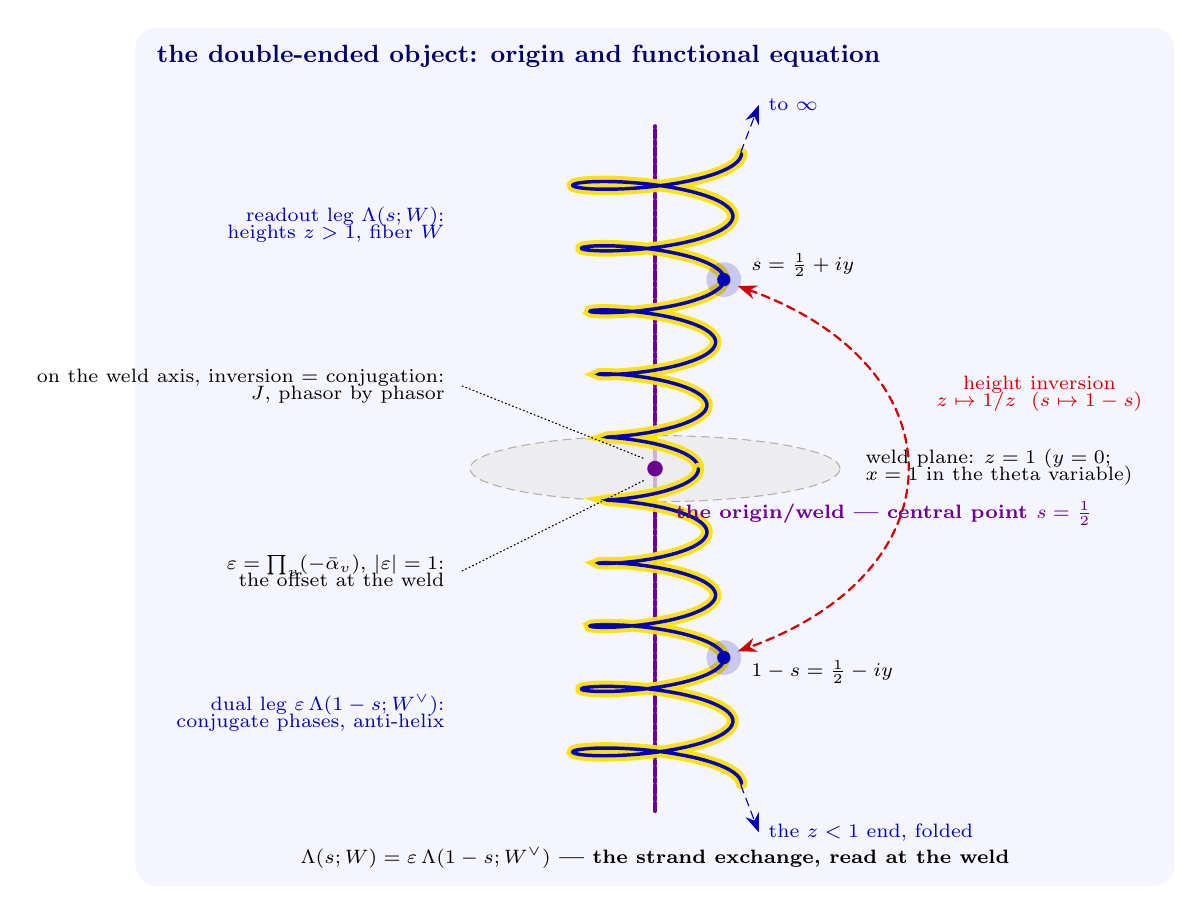
\begin{tikzpicture}[>={Stealth[length=2.4mm]}, line cap=round]
\colorlet{carrierY}{yellow!85!orange}
\colorlet{fiberB}{blue!72!black}
\colorlet{midV}{violet!85!blue}
\colorlet{vanishR}{red!82!black}
% ---- background ----
\fill[blue!4, rounded corners=8pt] (-6.6,-5.3) rectangle (6.6,5.6);
\node[anchor=north west, font=\bfseries\small, text=blue!40!black]
  at (-6.45,5.50) {the double-ended object: origin and functional equation};
% ---- weld axis (midline) ----
\draw[midV, line width=1.4pt, densely dash dot] (0,-4.35) -- (0,4.35);
% ---- weld plane at z=1 ----
\fill[gray!16, opacity=0.75] (0,0) ellipse [x radius=2.35, y radius=0.42];
\draw[gray!60, densely dashed] (0,0) ellipse [x radius=2.35, y radius=0.42];
\node[anchor=west, font=\scriptsize, align=left] at (2.55,0.02)
  {weld plane: $z=1$ ($y=0$;\\[-2pt]$x=1$ in the theta variable)};
% ---- upper helix: readout leg ----
\draw[carrierY, line width=4.2pt, opacity=0.95]
  plot[domain=0:1800, samples=320, smooth]
  ({(0.55+0.0003*\x)*cos(\x)}, {\x/450+0.2*(0.55+0.0003*\x)*sin(\x)});
\draw[fiberB, line width=1.25pt]
  plot[domain=0:1800, samples=320, smooth]
  ({(0.55+0.0003*\x)*cos(\x)}, {\x/450+0.2*(0.55+0.0003*\x)*sin(\x)});
% ---- lower anti-helix: dual leg (exact mirror through the weld) ----
\draw[carrierY, line width=4.2pt, opacity=0.95]
  plot[domain=0:1800, samples=320, smooth]
  ({(0.55+0.0003*\x)*cos(\x)}, {-\x/450-0.2*(0.55+0.0003*\x)*sin(\x)});
\draw[fiberB, line width=1.25pt]
  plot[domain=0:1800, samples=320, smooth]
  ({(0.55+0.0003*\x)*cos(\x)}, {-\x/450-0.2*(0.55+0.0003*\x)*sin(\x)});
% ---- origin / weld point ----
\fill[midV] (0,0) circle (2.8pt);
\node[midV, anchor=north west, font=\scriptsize\bfseries] at (0.14,-0.30)
  {the origin/weld --- central point $s=\tfrac12$};
% ---- continuations to infinity ----
\draw[fiberB, densely dashed, ->] (1.09,4.02) -- (1.32,4.62)
  node[anchor=west, font=\scriptsize] {to $\infty$};
\draw[fiberB, densely dashed, ->] (1.09,-4.02) -- (1.32,-4.62)
  node[anchor=west, font=\scriptsize] {the $z<1$ end, folded};
% ---- functional-equation reflection P <-> P^vee ----
\fill[fiberB, opacity=0.18] (0.874,2.4) circle (0.22);
\fill[fiberB, opacity=0.18] (0.874,-2.4) circle (0.22);
\fill[fiberB] (0.874,2.4) circle (2.4pt);
\fill[fiberB] (0.874,-2.4) circle (2.4pt);
\node[anchor=west, font=\scriptsize] at (1.10,2.58) {$s=\tfrac12+iy$};
\node[anchor=west, font=\scriptsize] at (1.10,-2.58) {$1-s=\tfrac12-iy$};
\draw[<->, vanishR, thick, densely dashed]
  (1.05,2.32) .. controls (3.9,1.3) and (3.9,-1.3) .. (1.05,-2.32);
\node[vanishR, align=center, font=\scriptsize, anchor=west] at (3.45,0.95)
  {height inversion\\[-2pt]$z\mapsto 1/z$ \ ($s\mapsto 1-s$)};
% ---- J and epsilon annotations (left) ----
\node[align=right, anchor=east, font=\scriptsize] at (-2.55,1.05)
  {on the weld axis, inversion $=$ conjugation:\\[-2pt]
   $J$, phasor by phasor};
\draw[densely dotted] (-2.45,1.05) -- (-0.12,0.12);
\node[align=right, anchor=east, font=\scriptsize] at (-2.55,-1.30)
  {$\varepsilon=\prod_v(-\bar\alpha_v)$, $|\varepsilon|=1$:\\[-2pt]
   the offset at the weld};
\draw[densely dotted] (-2.45,-1.30) -- (-0.12,-0.14);
% ---- leg labels ----
\node[align=right, anchor=east, font=\scriptsize, fiberB] at (-2.55,3.10)
  {readout leg $\Lambda(s;W)$:\\[-2pt]heights $z>1$, fiber $W$};
\node[align=right, anchor=east, font=\scriptsize, fiberB] at (-2.55,-3.10)
  {dual leg $\varepsilon\,\Lambda(1-s;W^{\vee})$:\\[-2pt]
   conjugate phases, anti-helix};
% ---- FE banner ----
\node[font=\scriptsize\bfseries] at (0,-4.95)
  {$\Lambda(s;W)=\varepsilon\,\Lambda(1-s;W^{\vee})$ --- the strand
   exchange, read at the weld};
\end{tikzpicture}}
\caption{Where the origin and the functional equation enter. The carrier is
double-ended: the readout leg (heights \(z>1\), fiber \(W\)) and the dual
leg (the \(z<1\) end, conjugate phases on the anti-helix, fiber
\(W^{\vee}\)) are welded at the origin \(z=1\) --- the central point
\(s=\tfrac12\), where the weld plane meets the weld axis. The functional
equation is the fold through that weld: height inversion \(z\mapsto1/z\)
(\(s\mapsto1-s\)) exchanges the legs, and on the weld axis the inversion
coincides with conjugation, which \(J\) supplies phasor by phasor
(Theorem~\ref{thm:carrierreflection}, Lemma~\ref{lem:bankreflection},
step~1) --- no Poisson summation is consumed. The only mismatch the exchange
permits is the unimodular offset at the weld,
\(\varepsilon=\prod_v(-\bar\alpha_v)\), assembled per place in Lean
(\texttt{StrandExchange.bankProduct\_exchange} from
\texttt{ChiralityHB.symClock\_star}); \(\varepsilon\) is the root number,
the offset that places or doubles the central cancellation.}
\label{fig:grh-weld}
\end{figure}

\subsection{The fiber: the character's occupation of the
carrier}\label{sec:grh-buckets}

The carrier is common; the \emph{fiber} is what a particular source puts on
it. A Dirichlet character \(\chi\bmod q\) attaches its fiber \(F_\chi\): one
phasor per integer per lane, with magnitude and phase synthesized from
\(\chi\)'s finite data alone
(Theorem~\ref{thm:g3-g4-identity-synthesis}) --- the phasor of \(n\) carries
the character phase \(\chi(n)\) on the carrier's winding at \(n\). The
carrier \emph{hosts} the fiber; it does not become it: the same carrier point
under two characters carries two different fiber states, distinguished by the
retained identity, and neither a shared carrier point nor a shared scalar
readout identifies two sources
(Corollary~\ref{cor:g3-complete-state-identity}). The 3D representation of
\(L(s,\chi)\) referred to throughout this part is the \emph{realized} fiber:
the complete state of Part~I --- carrier, fiber, native clock, native cells
--- specialized to the basic configuration.

Each phasor enters at its own height and at zero magnitude: the phasor of
\(n\) is born at height \(Z=n\) and grows continuously with height ---
there is no convergence gate on the carrier
(\S\ref{sec:grh-statespace}). The dual copy rides the anti-helix with the
same height law and conjugate transverse phase, so the two lanes run in
parallel, heights matching, geometries conjugate
(Theorem~\ref{thm:g1-double-carrier}).

The conductor decides the buckets. For \(n\) sharing a factor with \(q\) we
have \(\chi(n)=0\): the phasor is \emph{neutral} (U) --- present on the
carrier, silent in this character's readout. For \(n\) coprime to \(q\) the
character phase routes the phasor: a real character splits the units into a
\emph{positive} lane P (\(\chi(n)=+1\)) and a \emph{negative} lane M
(\(\chi(n)=-1\)); a complex character distributes its phases over the
\(\mu_6\)-cell directions, and the P/M split is realized as the signed channel
pair \((A,B)\) --- the \(\operatorname{Re}\)- and \(\operatorname{Im}\)-lanes
of the reflected readout (Theorem~\ref{thm:g6-mode-bridge}). The same integers
occupy the same carrier for every character; only the bucket assignment
changes. 

\subsection{The bidirectional transport: down to the ordinate, back to the
state}\label{sec:grh-projection}

The transport between the 3D state and the 1D chart runs in both directions,
each direction a named map, and both composites are the identity
(Theorem~\ref{thm:g2-ledgered-projection}). Neither direction is a metaphor:
down is how the classical function is read off the state, and up is how a
chart event is located back on the carrier.

\emph{Downward.} The descent is two coordinate suppressions and a logarithm.
Write a complete carrier coordinate state as \(\mathsf X=(r,\theta,z)\)
(\S\ref{sec:grh-statespace}). The first projection forgets the radius,
\[
\Pi_{32}(r,\theta,z)=(\theta,z),
\]
recording the two-dimensional carrier image --- in the reflected chart, the
Cayley/M\"obius image on the unit-circle chart
(Theorem~\ref{thm:carrierreflection}, item (P)). The second forgets the
phase,
\[
\Pi_{21}(\theta,z)=z,
\]
leaving the height alone. The analytic chart then reads the retained height
logarithmically,
\[
\Pi^{\log}_{21}(\theta,z)=\log z=y,
\]
and places it at the represented point \(\tfrac12+iy\) of the strip: the
abscissa supplied by the derived weld axis
(\S\S\ref{sec:grh-helix} and~\ref{sec:grh-midpoint-provenance}), the
ordinate by the logarithm of the height. That is
the whole downward mechanism. A three-dimensional value becomes a
one-dimensional ordinate by having its radius suppressed, its phase
suppressed, and its height passed through \(\log\). What is suppressed is
booked, not destroyed: each projection is paired with the loss ledger
\(\mathcal D(\mathsf X)=(r,\theta)\) --- in general: radius, angle, clock
offset, adapter state, every coordinate the chosen chart makes invisible.

\emph{Upward.} The ascent is reconstruction from the readout and the ledger,
and it is exact:
\[
\operatorname{Rec}\bigl(\Pi(\mathsf X),\mathcal D(\mathsf X)\bigr)=\mathsf X,
\qquad
\operatorname{Rec}^{\log}\bigl(y,(r,\theta)\bigr)=(r,\theta,e^{y}).
\]
A chart ordinate \(y\) lifts to the carrier height \(Z=e^{y}\); the ledger
restores the radius and phase; and the lift lands on the exact state the
projection left. This is a bijection with an explicit two-sided inverse ---
\(\texttt{record}\,f=(\text{height},(\text{radial},\text{phase}))\) inverts
by \texttt{reconstruct} and \texttt{reconstruct} inverts by \texttt{record}
(Lean \texttt{ConeProjection.record\_bijective}, \texttt{reconstruct\_record});
distinct helix events write distinct ledger entries
(\texttt{SourceHolonomy.projection\_bijective\_loss\_ledger}). Transport with
the ledger is lossless in both directions; transport without the ledger is a
compression, and provably so --- dropping the radial channel alone already
makes the projection non-injective (\texttt{ConeProjection.radial\_lost},
\S\ref{sec:grh-E1}).

The two directions do different work in this part. Downward is
\emph{reading}: the value of \(L(s,\chi)\) at the represented point
\(\tfrac12+iy\) is the final verification of a marked event --- the analytic
function is consulted after the event, never used to build it
(non-circularity, \S\ref{sec:grh-overview}). Upward is \emph{locating}: a
chart ordinate \(y\) names the carrier height \(e^{y}\) at which the operator
reads the bank, and the two reading-hypotheses of this part are statements
about precisely this lift --- the 1D-primary branch of the weak hypothesis is
the upward lift \(\gamma=\Im\rho\) landing on an eigenstate. The classical
analytic function is the downward readout \emph{without} the ledger --- the
ledger stays on the carrier. This is why equality of readouts does not imply
equality of states: two states share an ordinate whenever their heights
agree, whatever their radii and phases are doing; the exact criterion is that
readout \emph{plus ledger} determines the state
(Corollary~\ref{cor:g2-projected-equality}).

Both decisions of \S\ref{sec:grh-overview} take their teeth from this
mechanism. The 1D ordinate is the logged trace of the 3D event; the
eigenstate carries the coordinates the ordinate dropped. Whether an
eigenvalue must \emph{be} that trace or \emph{coincide} with it (decision
one), and whether the event or its trace is ``the zero'' (decision two), are
questions about the two ends of the maps displayed above.
Figure~\ref{fig:grh-pipeline} draws the entire pipeline for \(\chi_3\): the
conjugate pair up to its first crossing, and the ledgered descent to the
chart --- with the midline surviving every stage.

\begin{figure}[p]
\centering
\resizebox{\textwidth}{!}{%
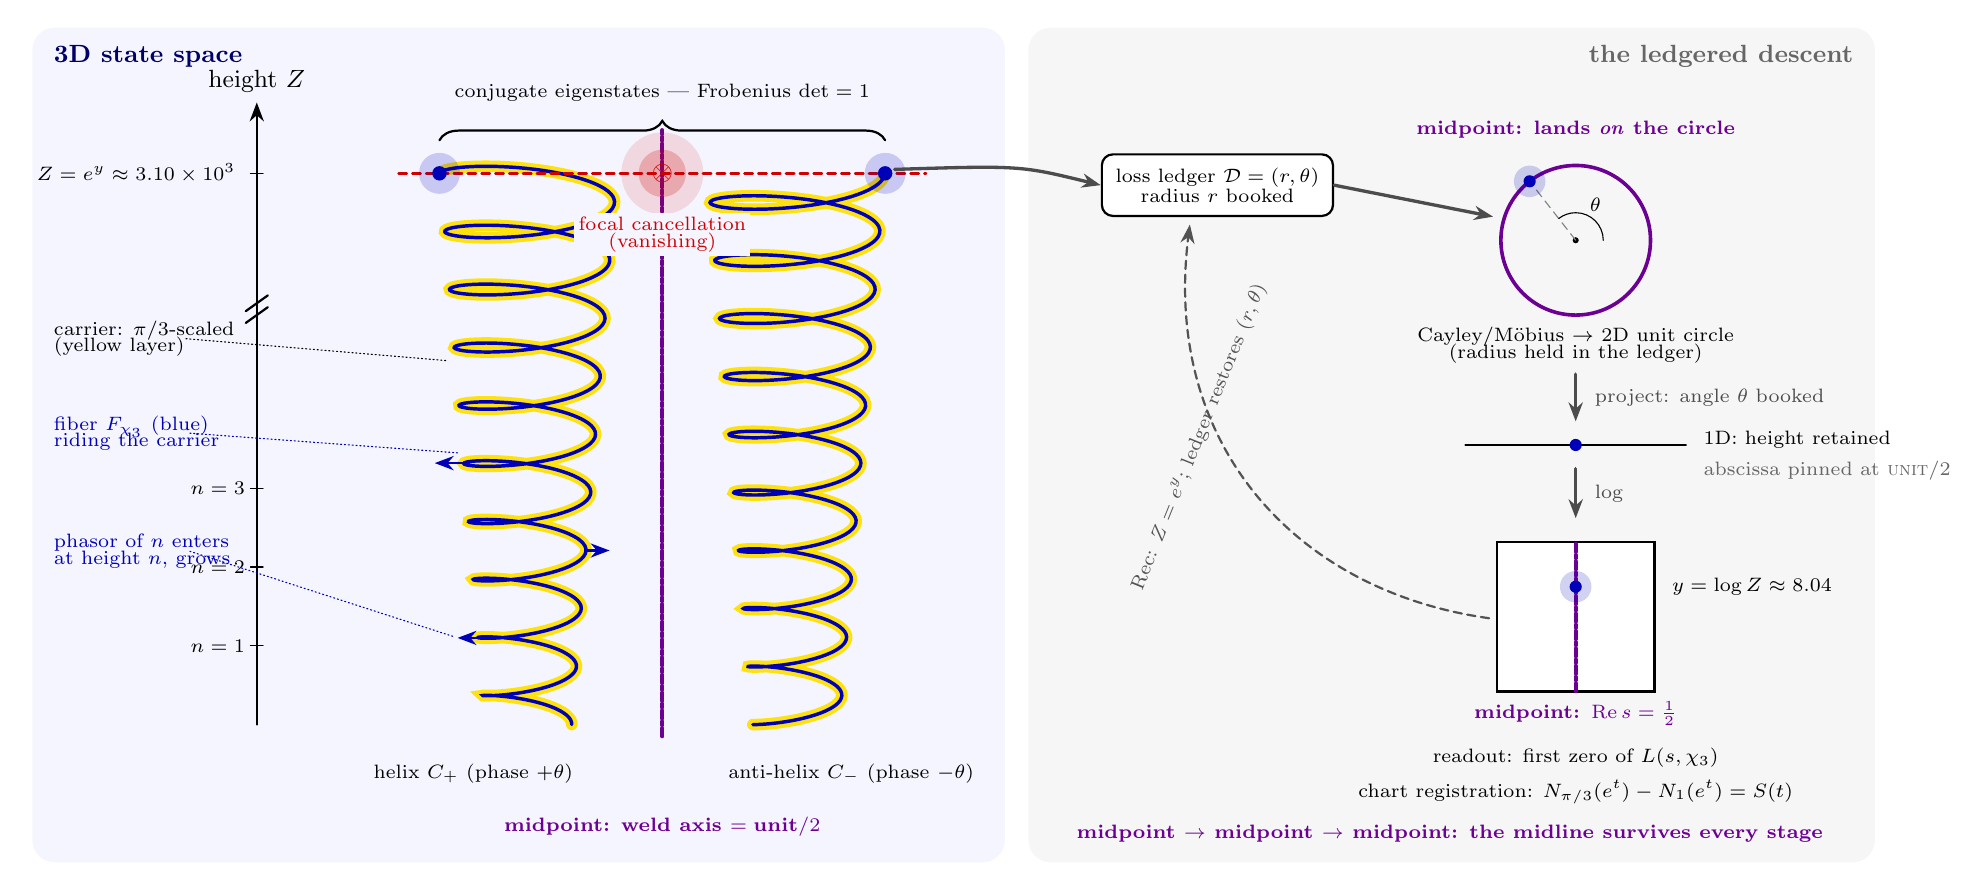
\begin{tikzpicture}[>={Stealth[length=2.4mm]}, line cap=round]
\colorlet{carrierY}{yellow!85!orange}
\colorlet{fiberB}{blue!72!black}
\colorlet{midV}{violet!85!blue}
\colorlet{vanishR}{red!82!black}
% ================= PANEL BACKGROUNDS =================
\fill[blue!4, rounded corners=8pt] (-8.0,-1.75) rectangle (4.35,8.85);
\fill[gray!7, rounded corners=8pt] (4.65,-1.75) rectangle (15.4,8.85);
\node[anchor=north west, font=\bfseries\small, text=blue!40!black]
  at (-7.85,8.75) {3D state space};
\node[anchor=north east, font=\bfseries\small, text=black!60]
  at (15.25,8.75) {the ledgered descent};
% ================= PANEL A: the 3D object =================
% weld axis: the midline, unit/2 (midpoint no. 1)
\draw[midV, line width=1.4pt, densely dash dot] (0,-0.15) -- (0,7.55);
\node[midV, font=\scriptsize\bfseries] at (0,-1.30)
  {midpoint: weld axis $=\textsc{unit}/2$};
% height axis
\draw[->, thick] (-5.15,0) -- (-5.15,7.9) node[above] {\small height $Z$};
\foreach \n in {1,2,3}{
  \draw (-5.23,\n) -- (-5.07,\n) node[left=3pt] {\scriptsize $n=\n$};}
\draw[thick] (-5.29,5.25) -- (-5.01,5.45);
\draw[thick] (-5.29,5.10) -- (-5.01,5.30);
\draw (-5.23,7) -- (-5.07,7);
\node[anchor=east, font=\scriptsize] at (-5.30,7)
  {$Z=e^{y}\approx 3.10\times10^{3}$};
% ---- helix C+ (left): yellow carrier band, blue fiber riding it ----
\draw[carrierY, line width=4.2pt, opacity=0.95]
  plot[domain=0:3420, samples=480, smooth]
  ({-1.7+(0.55+0.00017*\x)*cos(\x)}, {\x/488.57+0.22*(0.55+0.00017*\x)*sin(\x)});
\draw[fiberB, line width=1.25pt]
  plot[domain=0:3420, samples=480, smooth]
  ({-1.7+(0.55+0.00017*\x)*cos(\x)}, {\x/488.57+0.22*(0.55+0.00017*\x)*sin(\x)});
% ---- anti-helix C- (right, mirrored winding, conjugate tilt) ----
\draw[carrierY, line width=4.2pt, opacity=0.95]
  plot[domain=0:3420, samples=480, smooth]
  ({1.7-(0.55+0.00017*\x)*cos(\x)}, {\x/488.57-0.22*(0.55+0.00017*\x)*sin(\x)});
\draw[fiberB, line width=1.25pt]
  plot[domain=0:3420, samples=480, smooth]
  ({1.7-(0.55+0.00017*\x)*cos(\x)}, {\x/488.57-0.22*(0.55+0.00017*\x)*sin(\x)});
% ---- phasor entries on C+ ----
\draw[->, fiberB, thick] (-2.34,1.10) -- ++(-0.26,0);
\draw[->, fiberB, thick] (-0.97,2.21) -- ++(0.30,0);
\draw[->, fiberB, thick] (-2.53,3.32) -- ++(-0.36,0);
% ---- left label stack ----
\node[align=left, anchor=west, font=\scriptsize] at (-7.85,4.90)
  {carrier: $\pi/3$-scaled\\[-2pt](yellow layer)};
\draw[densely dotted] (-6.05,4.90) -- (-2.72,4.62);
\node[align=left, anchor=west, font=\scriptsize, fiberB] at (-7.85,3.70)
  {fiber $F_{\chi_3}$ (blue)\\[-2pt]riding the carrier};
\draw[fiberB, densely dotted] (-6.00,3.70) -- (-2.60,3.45);
\node[fiberB, align=left, anchor=west, font=\scriptsize] at (-7.85,2.20)
  {phasor of $n$ enters\\[-2pt]at height $n$, grows};
\draw[fiberB, densely dotted] (-6.00,2.20) -- (-2.66,1.12);
% ---- crossing / focal cancellation (glow) ----
\fill[vanishR, opacity=0.12] (0,7) circle (0.52);
\fill[vanishR, opacity=0.22] (0,7) circle (0.30);
\draw[vanishR, densely dashed, line width=0.9pt] (-3.35,7) -- (3.35,7);
\fill[fiberB, opacity=0.18] (-2.83,7) circle (0.26);
\fill[fiberB, opacity=0.18] (2.83,7) circle (0.26);
\fill[fiberB] (-2.83,7) circle (2.6pt);
\fill[fiberB] (2.83,7) circle (2.6pt);
\node[vanishR] at (0,7) {$\otimes$};
\node[vanishR, align=center, font=\scriptsize, fill=blue!4, inner sep=1.5pt]
  at (0,6.22) {focal cancellation\\[-2pt](vanishing)};
% ---- Frobenius bracket ----
\draw[decorate, decoration={brace, amplitude=7pt}, thick]
  (-2.83,7.42) -- (2.83,7.42);
\node[font=\scriptsize] at (0,8.02)
  {conjugate eigenstates --- Frobenius $\det=1$};
% ---- lane labels ----
\node[font=\scriptsize] at (-2.4,-0.62) {helix $C_{+}$ (phase $+\theta$)};
\node[font=\scriptsize] at (2.4,-0.62) {anti-helix $C_{-}$ (phase $-\theta$)};
% ================= PANEL B: the ledgered descent =================
% ledger box
\node[draw, thick, rounded corners, align=center, inner sep=5pt,
      fill=white, font=\scriptsize] (ledger) at (7.05,6.85)
  {loss ledger $\mathcal D=(r,\theta)$\\[-1pt]radius $r$ booked};
\draw[->, very thick, black!70] (2.95,7.05) .. controls (4.55,7.10) .. (ledger.west);
% ---- 2D stage: unit circle (midpoint no. 2) ----
\draw[midV, line width=1.3pt] (11.6,6.15) circle (0.95);
\fill (11.6,6.15) circle (1.1pt);
\draw[gray, densely dashed] (11.6,6.15) -- ++(128:0.95);
\fill[fiberB, opacity=0.18] ($(11.6,6.15)+(128:0.95)$) circle (0.2);
\fill[fiberB] ($(11.6,6.15)+(128:0.95)$) circle (2.2pt);
\draw (11.95,6.15) arc[start angle=0, end angle=128, radius=0.35];
\node[font=\scriptsize] at (11.85,6.60) {$\theta$};
\node[align=center, font=\scriptsize] at (11.6,4.82)
  {Cayley/M\"obius $\to$ 2D unit circle\\[-2pt](radius held in the ledger)};
\node[midV, font=\scriptsize\bfseries, align=center] at (11.6,7.55)
  {midpoint: lands \emph{on} the circle};
\draw[->, very thick, black!70] (ledger.east) -- (10.55,6.45);
% ---- 1D stage ----
\draw[->, very thick, black!70] (11.6,4.45) -- (11.6,3.85)
  node[midway, right=3pt, font=\scriptsize] {project: angle $\theta$ booked};
\draw[thick] (10.2,3.55) -- (13.0,3.55);
\fill[fiberB] (11.6,3.55) circle (2.2pt);
\node[anchor=west, font=\scriptsize] at (13.1,3.62)
  {1D: height retained};
\node[anchor=west, font=\scriptsize, text=black!60] at (13.1,3.22)
  {abscissa pinned at $\textsc{unit}/2$};
% ---- chart stage (midpoint no. 3) ----
\draw[->, very thick, black!70] (11.6,3.25) -- (11.6,2.62)
  node[midway, right=3pt, font=\scriptsize] {$\log$};
\fill[white] (10.6,0.42) rectangle (12.6,2.32);
\draw[thick] (10.6,0.42) rectangle (12.6,2.32);
\draw[midV, line width=1.3pt, densely dash dot] (11.6,0.42) -- (11.6,2.32);
\fill[fiberB, opacity=0.18] (11.6,1.75) circle (0.2);
\fill[fiberB] (11.6,1.75) circle (2.2pt);
\node[anchor=west, font=\scriptsize] at (12.7,1.75)
  {$y=\log Z\approx 8.04$};
\node[midV, font=\scriptsize\bfseries] at (11.6,0.14)
  {midpoint: $\Re s=\tfrac12$};
\node[font=\scriptsize] at (11.6,-0.42)
  {readout: first zero of $L(s,\chi_3)$};
\node[font=\scriptsize] at (11.6,-0.86)
  {chart registration: $N_{\pi/3}(e^{t})-N_{1}(e^{t})=S(t)$};
% ---- return arrow (bidirectional transport) ----
\draw[->, densely dashed, thick, gray!65!black]
  (10.5,1.35) .. controls (8.0,1.7) and (6.35,3.6) .. (6.70,6.35);
\node[gray!65!black, align=center, rotate=68, font=\scriptsize] at (6.82,3.65)
  {$\operatorname{Rec}$: $Z=e^{y}$; ledger restores $(r,\theta)$};
% ---- midline thread annotation ----
\node[midV, font=\scriptsize\bfseries] at (10.0,-1.38)
  {midpoint $\to$ midpoint $\to$ midpoint: the midline survives every stage};
\end{tikzpicture}}
\caption{The pipeline for \(\chi_3\), end to end (heights schematic, not to
scale). \emph{Left panel} --- the 3D object: helix \(C_{+}\) and conjugate
anti-helix \(C_{-}\), the \(\pi/3\)-scaled carrier as the yellow layer, the
fiber \(F_{\chi_3}\) in blue growing from the origin with phasors entering
at integer heights; the violet dash-dot line is the weld axis --- the
midline at \(\textsc{unit}/2\), the fixed locus of \(J\). At the first
crossing the lanes align in exact focal cancellation, and the conjugate
eigenstate pair (Frobenius \(\det=1\)) marks the event at height
\(Z=e^{y}\approx3.10\times10^{3}\). \emph{Right panel} --- the ledgered
descent: radius booked in the loss ledger, Cayley/M\"obius to the 2D unit
circle, angle booked at the projection to 1D, logarithm to the chart,
landing the readout at \(y=\log Z\approx 8.0397\), the first zero of
\(L(s,\chi_3)\), with \(S(t)\) the registration bookkeeping between the two
scales (\S\ref{sec:carrier-S}). The violet thread is the midline surviving
every stage --- weld axis in 3D, on-circle landing in 2D
(\texttt{midpoint\_entry\_on\_circle}), \(\Re s=\tfrac12\) in the chart
(\texttt{pipeline\_midpoint\_iff}): the ordinate compresses by a logarithm
while the abscissa is first derived by the area law and then held by
no-drift symmetry. The dashed return arrow is the
upward transport: readout plus ledger reconstructs the state exactly
(\S\ref{sec:grh-projection}).}
\label{fig:grh-pipeline}
\end{figure}

% Midpoint audit searches run 2026-07-14:
% rg -n -i "carrierPoint|carrier_point|ThreeD_crossings_are_real_zeros|three_d_crossings_are_real_zeros|crossings.*real.*zeros|ThreeDZero|three_d_zero|no.?drift|drift.?zero|offline|off.?line|off.?carrier|midpoint|half.?unit|area.?law|archimedean.*helix|helix.*archimedean" . --glob '*.lean' --glob '*.tex' --glob '!staging_rp2/**'
% rg -n -i "(no.*drift|drift.*zero|drift.*iff|scaleBalanced_iff|sigma_half_is_scale_critical|carrier.*offline|offline.*carrier|cancellation.*offline|offline.*cancellation|admissible.*offline|offline.*admissible|reprPoint|spectralCoord|carrierPoint|pipeline_midpoint_iff)" RequestProject --glob '*.lean'
% rg -n -i "carrierPoint|carrier_point|ThreeD_crossings_are_real_zeros|three_d_crossings_are_real_zeros|ThreeDZero|three_d_zero|no_radial_drift_on_helix|helix_no_offline_cancellation|sigma_half_is_scale_critical|scaleBalanced_iff" .lake/packages/mathlib/Mathlib --glob '*.lean'

\subsection{Midpoint provenance: geometry first, chart second}
\label{sec:grh-midpoint-provenance}

The order of construction matters here.  The carrier is not introduced as
the vertical line \(\Re s=\tfrac12\).  Before there is an \(s\)-plane, a
zero \(\rho\), or a definition of \texttt{carrierPoint}, the wound integer
line has a cylindrical radius \(r_n\).  The arclength calculation gives
\[
  \frac{r_n^2}{n}\longrightarrow \frac{r\Delta}{\pi}>0,
  \qquad
  \frac{r_n}{\sqrt n}\longrightarrow
     \sqrt{\frac{r\Delta}{\pi}}>0
\]
(\texttt{windIntegerSite\_radius\_sq\_tendsto} and
\texttt{carrierRadius\_div\_sqrt\_tendsto}).  Thus the exponent
\(\sigma\) of a fiber amplitude \(n^{-\sigma}\) is initially free.  Define
geometric admissibility by the existence of a finite positive scale limit,
\[
 \operatorname{ScaleBalanced}(\sigma)
 \quad:\Longleftrightarrow\quad
 \exists L>0,
 \quad n^{-\sigma}r_n\longrightarrow L.
\]
The area law then proves
\[
 \operatorname{ScaleBalanced}(\sigma)
 \quad\Longleftrightarrow\quad
 \sigma=\frac12.
 \tag{MP1}\label{eq:grh-midpoint-area-law}
\]
This is \texttt{sigma\_half\_is\_scale\_critical}, re-exported as
\texttt{scaleBalanced\_iff}.  The gauge parameters \(r\) and \(\Delta\)
change the positive limiting constant, but not the exponent.  Consequently
the midpoint is an output of the three-dimensional arclength geometry: it
is the exponent of the square-root radius, not a coordinate selected from
the analytic zero set.

There is an independent no-drift form of the same conclusion.  A raw
source mode has a complex transport rate \(\lambda\) and nonzero amplitude
\(a\), with conservation law
\[
  e^{(\Re\lambda)\tau}a=a\qquad(\tau\in\mathbb R).
\]
Taking \(\tau=1\) forces \(\Re\lambda=0\)
(\texttt{source\_noDrift} and \texttt{SourceMode.noDrift}).  This statement
contains no \(\rho\), no \(s\), and no numerical midpoint.  In the radial
normalization supplied by (MP1), a putative abscissa \(\sigma\) has residual
drift \(n^{\sigma-\sigma_*}\), where
\(\sigma_*\) is the unique scale-balanced exponent.  Hence
\[
  n^{\sigma-\sigma_*}=1\ (n>1)
  \quad\Longleftrightarrow\quad \sigma=\sigma_*
  \quad\Longleftrightarrow\quad \sigma=\frac12,
 \tag{MP2}\label{eq:grh-midpoint-drift}
\]
the compiled specialization being
\texttt{Helix.no\_radial\_drift\_iff\_half}.  Thus the two inputs agree:
the area law determines the centre \(\sigma_*\), and conservation prohibits
motion away from it.

Only after (MP1)--(MP2) is the spectral chart attached.  The physical height
and its internal logarithmic ordinate are
\[
 Z>0,\qquad y=\log Z,\qquad
 \operatorname{carrierPointAtHeight}(Z)=\sigma_*+i\log Z.
\]
Lean stores the ordinate chart and physical-height readout separately:
\[
\begin{aligned}
 \texttt{carrierPoint y}&:=\texttt{carrierAbscissa}+iy,\\
 \texttt{carrierPointAtHeight Z}&:=\texttt{carrierPoint}(\log Z).
\end{aligned}
\]
Here \texttt{carrierAbscissa} is selected from the unique witness of
\texttt{CarrierScaleBalanced}; only the theorem
\texttt{carrierAbscissa\_eq\_half} rewrites it to \(\tfrac12\).  The theorem
\texttt{carrierPoint\_eq\_half\_add\_I} is therefore a downstream normal-form
lemma, not the definition of the carrier coordinate.  Theorems
\texttt{carrierPointAtHeight\_im} and
\texttt{carrierPointAtHeight\_exp} certify $y=\log Z$ and
$Z=e^y$ in both directions.

The completed native crossing is
\[
\texttt{CompletedThreeDZeroAtHeight}\ \chi\ Z
 \quad:\Longleftrightarrow\quad
 Z>0\ \wedge\ \texttt{Dcell}\ \chi\ Z=0.
\]
The exact representation theorem gives
\[
 \texttt{CompletedThreeDZeroAtHeight}\ \chi\ Z
 \Longleftrightarrow
 L(\sigma_*+i\log Z,\chi)=0.
\]
The finite declaration \texttt{ThreeDZero} remains the truncated
ordinate-level focal closure used by the finite pencil proofs.

Two exclusion theorems make the image statement exact.  First,
\texttt{not\_scaleBalanced\_of\_ne} says that an abscissa different from
\(\sigma_*\) is not a native carrier state.  Second,
\texttt{helix\_no\_offline\_cancellation} says that an off-circle Cayley
ledger entry cannot be produced by a weld-fixed helix event, while
\texttt{projection\_bijective\_loss\_ledger} says that the height-to-ledger
map is injective on the carrier image.  Projection can therefore neither
move a native cancellation away from the midpoint nor merge two carrier
events into a counterfeit cancellation.  An off-midpoint analytic
vanishing, if presented to this 3D representation, has no scale-balanced,
drift-free carrier source.

This also separates the exact logical role of
\texttt{ThreeD\_crossings\_are\_real\_zeros}.  Its clause
\(\rho=\texttt{carrierPointAtHeight}(Z)\) is the
\emph{coverage/identification}
assertion that a classical analytic zero belongs to the carrier image.  It
is not the derivation of that image's real coordinate: (MP1)--(MP2) and the
exclusion theorems have already done that without quantifying over analytic
zeros.  Once coverage is granted, taking real parts is of course immediate;
the substantive interface question is whether every analytic zero is
represented by a native focal event.  The paper will use
\texttt{carrierPoint} only in this downstream, normal-form sense.  Lean makes
the separation executable by defining the midpoint-free statement
\texttt{NativeCarrierCoverage} and proving
\[
 \texttt{ThreeD\_crossings\_are\_real\_zeros}(\chi)
 \leftrightarrow
 \mathrm{GRH}(\chi)\wedge\texttt{NativeCarrierCoverage}(\chi).
\]
Consequently the legacy equality premise is not cited as evidence for the
coverage direction; an unconditional closure must discharge the midpoint-free
coverage proposition (or the fixed-operator spectral-capture interface)
directly.

\subsection{The chart: \texorpdfstring{\(y=\log Z\) and
\(Z=e^{y}\)}{y = log Z and Z = e\^{}y}}\label{sec:grh-chart}

The readout just constructed does not live at the carrier's scale. The
identity between the scales is one equation read in both directions:
downward, the chart ordinate is the logarithm of the carrier height,
\(y=\log Z\); upward, the carrier height is the exponential of the chart
ordinate, \(Z=e^{y}\). A carrier state at height \(Z>0\) is read at the
represented point \(\tfrac12+iy\) (\texttt{HarmonicPencilCell.reprPoint});
the phasor of the integer \(n\), born at height \(n\), is charted at
ordinate \(\log n\). The compression this induces is the single most
important fact about the relation between the two representations. At the
first zero of \(\zeta\), the chart reads \(y=14.1347\ldots\); the carrier
height is \(Z=e^{y}\approx1.38\times10^{6}\), and the realized bank below
that height already holds about \(1.38\) million integer phasors per lane.
In general the chart ordinate \(y\) summarizes a bank of
\(\lfloor e^{y}\rfloor\) phasors in one complex number. The 1D representation
is not a smaller copy of the 3D representation; it is a logarithmically
compressed summary of the same function, and the scale mismatch between the
two charts is itself a theorem-level object (\S\ref{sec:carrier-S}).

The abscissa tells the same story from the other side.  The carrier's
arclength law first derives the unique scale-balanced exponent
\(\sigma_*=\tfrac12\), and conservation then fixes every native mode at zero
radial drift (\S\ref{sec:grh-midpoint-provenance}).  Riemann's substitution
\(s=\tfrac12+ti\) is the analytic chart of that derived weld axis, and the
represented point \(\sigma_*+iy=\tfrac12+iy\) simply reads height along it.
The ordinate compresses by a logarithm while the abscissa is pinned by a
geometric scale law and its no-drift conservation --- which is why every
subsequent argument in this part is an argument about heights.  The midline
has already been located before the chart is defined.

\subsection{Vanishing is focal alignment}\label{sec:grh-focal}

A zero, on the carrier, is not a value creeping down to nothing; it is an
alignment event. At a marked height the accumulated bank achieves exact
harmonic cancellation: the P and M lanes balance, the \(\mu_6\) cells close in
\(\mathbb Z[\zeta_6]\), and the residual carries no independent constant mode
--- the normalized cell residual factors as \(\det(L^{\mathrm c})/A=
(\lambda-\mu)B\) with \(\lambda-\mu\neq0\), so the residual vanishes exactly
when the signed closure channel does (Theorem~\ref{thm:g6-mode-bridge}).
The event is registered by rank at both exact levels.  At physical helix
height \(Z>0\), with logarithmic ordinate \(y=\log Z\), the canonical finite
bank closes exactly iff its spatially lifted harmonic Gram matrix drops rank
(\texttt{threeDZeroAtHeight\_twoGram3D\_rankDrop}).  This finite event is the
truncated detector \texttt{ThreeDZeroAtHeight}.  The completed fibre event is
\texttt{CompletedThreeDZeroAtHeight}; Lean proves
\[
 \texttt{CompletedThreeDZeroAtHeight}\ \chi\ Z
 \quad\Longleftrightarrow\quad
 L(\sigma_*+i\log Z,\chi)=0
\]
by \texttt{completedThreeDZeroAtHeight\_iff\_L\_zero}.  The theorem
\[
\texttt{completedHarmonicGram3DAtHeight\_rankDrop\_iff\_L\_zero}
\]
proves directly that its completed spatial harmonic Gram lift drops rank exactly at
that represented \(L\)-zero.  Thus the
3D crossing is focal cancellation in the completed \(L\)-function fibre at
physical height \(Z\); it is not inferred from a 1D chart criterion.  The
finite bank theorem is retained as its internal truncation-level detector and
is not substituted for the completed identity.

\medskip
\noindent\textbf{Note (Frobenius determinant one).} The conjugate eigenstate pair the alignment
realizes is not free to sit anywhere; it is pinned by an algebraic constraint. On the carrier the
local Frobenius acts as a \emph{similitude of determinant one}: its chiral block has \(\det=1\)
(\texttt{RequestProject/FrobeniusSimilitude.lean}, \texttt{frobeniusBlock\_det\_one}), so its two
eigenvalues multiply to one --- a reciprocal pair \(\{\alpha,\alpha^{-1}\}\). With the class
unitary they lie on the unit circle as a conjugate pair \(\{e^{i\theta},e^{-i\theta}\}\), and the
eigenphases \(\pm\theta\) are real: the algebraic reason the eigenstate pair is symmetric about the
weld axis rather than drifting off it. This is the carrier's realization of the classical
unit-circle normalization of the Satake--Frobenius class; on the analytic side it is Deligne's
purity, which places the normalized Frobenius eigenvalues on the unit circle \cite{Deligne}, with
the trivial similitude factor \(\det=1\) keeping them a conjugate pair. The one setting where this
mechanism is already a completed theorem is the function-field analog: Weil's Riemann hypothesis for
curves over a finite field \(\mathbb F_q\) is precisely the statement that the Frobenius eigenvalues
on the Jacobian have absolute value \(q^{1/2}\) and pair as \(\{\alpha,q/\alpha\}\), which after
normalization sit as conjugate pairs \(\{\beta,\beta^{-1}\}\) of determinant one on the unit circle
--- forcing the zeros of the congruence zeta function onto \(\Re s=\tfrac12\) \cite{Weil}; Deligne's
proof of the Weil conjectures extends this purity to smooth projective varieties of every dimension
\cite{Deligne}. There the Frobenius \emph{is} the operator whose spectrum pins the zeros to the
critical line, and determinant-one unitarity is the entire content of that conclusion --- the
carrier's \(\det=1\) block is the local, archimedean shadow of the same mechanism. We claim the
analog, not the classical case: the finite-field statement is an unconditional theorem, the
classical one is not, and importing the former as a proof of the latter is exactly the elision this
part refuses. The determinant-one fact is
a structural property of the representation, proven on the carrier; it does not by itself adjudicate
the naming decisions of \S\ref{sec:grh-overview} --- it fixes where the paired eigenphases live, not
which of \((\text{Z-3D})\)/\((\text{Z-1D})\) names the zero.

\subsection{The two Gram operators}\label{sec:grh-operators}

Two operators read the bank, and they divide the labor.

\emph{The Gram harmonic pencil} is the finite detector: the \(2\times2\)
pencil
\(L^{\mathrm c}=\left[\begin{smallmatrix}A&B\\ \mu A&\lambda
B\end{smallmatrix}\right]\)
on the signed channels, whose determinant vanishes --- whose rank drops ---
exactly at the alignment events (\S\ref{sec:grh-focal}). It is the instrument
that marks native focal-event heights on the carrier.

\emph{The local von Neumann fibre} is the coordinate-reading object. At each
physical 3D height \(Z>0\), its spectral parameter is the logarithmic ordinate
\(\gamma=y=\log Z\), and it is multiplication by \(\log Z\) on the
one-dimensional fibre,
\[
\texttt{vonNeumannOp}(\log Z)=(\log Z:\mathbb C)\cdot\mathrm{id},
\]
symmetric --- hence self-adjoint, with real spectrum \(\{\log Z\}\) --- as a
theorem, not an assumption (\texttt{vonNeumannOp\_isSymmetric},
\texttt{RequestProject/ClosedForm.lean}). The spectral parametrization sends
a real eigenvalue \(\mu\) to the represented point
\(\sigma_*+i\mu=\tfrac12+i\mu\), where \(\sigma_*\) has already been fixed
by (MP1).

Because a separate scalar operator is supplied for each \(\gamma\), this family is
not itself the one fixed operator required by the global Hilbert--P\'olya
interface.  Its exact role is to verify the local kernel and the reality of an
already supplied height.

The family is assembled, without changing any local proof, by the fixed
ambient carrier operator \(A^{(3)}_{p,r}\) above.  Its basis is indexed by all
geometric states $X=\gamma_{p,r}(y)$, independently of crossings, and
\(A^{(3)}_{p,r}\delta_X=y\delta_X\).  A completed 3D crossing
$e=(Z_e,h_e)$ selects the state $X_e=\gamma_{p,r}(\log Z_e)$ and Lean proves
that its physical third coordinate is $Z_e$.  Hence a ``3D eigenvector'' in
the ambient resolvent statements below means this explicit carrier basis state, while
\(\texttt{vonNeumannOp}(\log Z_e)\) computes its local
one-dimensional resolvent factor.

The internal 3D chain runs entirely on these two instruments, and every link
is unconditionally proven.  Finite focal cancellation at ordinate
\(y=\log Z\) is detected by the finite harmonic Gram rank drop.  Completed
focal cancellation at physical height \(Z\) is exactly the analytic
\(L\)-zero of that fibre and is detected by the completed harmonic Gram rank
drop.  The spatial statement
\texttt{completedThreeDZeroAtHeight\_twoGram3D\_rankDrop} supplies both the
completed harmonic rank drop and the von Neumann rank drop at the same
ordinate \(\log Z\).  The carrier point
\(\sigma_*+i\log Z=\tfrac12+i\log Z\) lies on the midline because the area law has
already proved \(\sigma_*=\tfrac12\), while von Neumann reality supplies the
real spectral ordinate and hence zero source drift
(\S\ref{sec:grh-midpoint-provenance}).  The one-line Lean proof
\texttt{simp [carrierPoint]} in \texttt{threeDZero\_on\_midline} is now
backed by \texttt{carrierAbscissa\_eq\_half} and is a
normal-form check, not the provenance of the half. Thus focal
cancellation \(=\) 3D zero \(\to\) harmonic Gram rank drop plus von Neumann
Gram rank drop at \(y=\log Z\): that is the detecting and realizing
instrument of this part, and no step consults the chart.

The same-event assertion is now a single compiled assembly theorem, rather
than an inference made in prose.  The theorem
\texttt{completedThreeDZeroAtHeight\_focal\_rankDrop\_eigenvector\_noRadialDrift}
returns, from a completed 3D event at physical height \(Z\), its focal residual
zero, spatial harmonic-pencil rank drop, nonzero ambient eigenvector with
eigenvalue \(\log Z\), and zero radial drift.  Its last component is proved by
\texttt{carrierPointAtHeight\_noRadialDrift}, which uses only that the readout
is a point of the area-law carrier.  Moreover,
\texttt{PrincipalContourNative3DCertificate.analyticFiber\_eq\_carrierFiber}
identifies the literal three-dimensional \(L\)-fiber at \(\rho\) with the
fiber at that certificate's marked carrier height, and the companion theorem
\texttt{.noRadialDrift} transports the geometric no-drift result to the
original analytic parameter.  Thus no-drift is an output of native helix
realization, not an extra condition attached to a zero.
More precisely, the compiled equality
\texttt{eventHeight\_eq\_focalCancellationHeight} identifies the event's
physical height with the literal analytic fiber's stored cancellation height.
The theorem \texttt{harmonicRankDrop\_at\_focalCancellationHeight} rewrites the
completed pencil by this equality before applying its rank-drop certificate;
it does not detect a second event having the same ordinate.  Finally,
\texttt{focalCancellation\_rankDrop\_noRadialDrift\_sameHeight} packages the
readout closure, the determinant zero, and the carrier no-drift law at that one
physical height.

The resolvent trace now has two event-typed versions
(\texttt{RequestProject/TwinResolventTrace.lean}).  For a finite
\(E\subset\mathcal E_\chi\), multiplicities \(m_e\), and
\(p(Z)=\texttt{carrierPointAtHeight}(Z)\), Version~I is
\[
 T^{(3)}_{\chi,E}(w)
 =\sum_{e\in E}m_e\,
   \texttt{vonNeumannResolventTrace}(\log Z_e,w)
 =\sum_{e\in E}\frac{m_e}{w-p(Z_e)}.
\]
The compiled ambient bundle
\texttt{threeDZero\_ambientEigenvector\_resolventTrace} states together that every
index \(e\) is a completed 3D zero, that \(\delta_e\ne0\) is its eigenvector
of \(A^{(3)}_{p,r}\), and that the displayed carrier-point trace formula
holds.  This is precisely the ``3D zeros plus 3D eigenvectors'' version.

Version~II reads the same certified events in the ordinate chart:
\[
 T^{(1\leftrightarrow3)}_{\chi,E}(u)
 =\sum_{e\in E}\frac{m_e}{\log Z_e-u}.
\]
The ambient bundle
\texttt{oneDZero\_threeDZero\_ambientEigenvector\_resolventTrace} additionally
proves, for every \(e\),
\[
 L\!\left(p(Z_e),\chi\right)=0,
 \qquad
 \texttt{CompletedThreeDZeroAtHeight}\ \chi\ Z_e,
 \qquad
 A^{(3)}_\chi\delta_e=(\log Z_e)\delta_e.
\]
The first equation is obtained from the completed focal residual by
\texttt{completedThreeDEigenEvent\_L\_zero}; it is not inserted as a second
unrelated zero assumption.  Finally Lean proves the exact chart relation
\[
 T^{(3)}_{\chi,E}(\texttt{lineC}(u))
 =i\,T^{(1\leftrightarrow3)}_{\chi,E}(u)
 \quad(\texttt{completedTraces\_agree}).
\]
The factor \(i\) is \(d(\texttt{lineC})/du\), and the two pole coordinates
are \(p(Z_e)=\sigma_*+i\log Z_e\) and \(\log Z_e\), respectively.  The older
abstract finite-set results \texttt{trace3D\_capture},
\texttt{trace3D\_analyticAt\_off}, \texttt{trace1D\_capture}, and
\texttt{twinTraces\_agree\_on\_window} remain in place; the new theorems
identify the 3D zero and eigenvector data that their abstract ordinate set did
not itself carry.

\subsection{The chart-side registration audit}\label{sec:grh-audit}

One further object appears in the evidence dossiers and deserves an exact
label. Over a finite window \((0,T]\), the Lean development builds a
diagonal matrix on the window's zero-events --- \(\texttt{hpOperator}\ T\),
one axis per unit of multiplicity, eigenvalue the event ordinate. Its name
is historical; its role is not spectral detection. It is a finite
\emph{repackaging of the already-located analytic zero window}, used for
exactly one thing: auditing the chart against the carrier, count and
multiplicity. The audit facts are proven and exact --- the diagonal is
Hermitian by type (\texttt{hpOperator\_isHermitian}); every index is an
exact vanishing (\texttt{eigenheight\_is\_exact\_vanishing}); the chart
reads zero at a height iff an index sits there
(\texttt{chartZero\_iff\_eigenheight}); the diagonal's dimension is the
chart's own count formula \(1+\theta(T)/\pi+S_{\mathrm{mult}}(T)\)
(\texttt{hpDimension\_eq\_registration}); the eigenspace dimension at an
event equals the vanishing order --- the mode space is a graded local
algebra \(\mathbb C[X]/((X-\mathrm{line}\,\gamma)^{\mathrm{ord}})\)
(\texttt{finrank\_modeSpace}), a double zero a two-dimensional crossing;
and the window traces are honest analytic objects
(\texttt{gradedResolventTrace\_eq\_residue\_sum},
\texttt{windowedDiffResolvent\_tendsto}). But because the window is indexed
by already-located analytic zeros, nothing in this subsection participates
in locating an event.  The local von Neumann fibre of
\S\ref{sec:grh-operators} likewise verifies an event after its height is
supplied.  The fixed global operator interface is stated separately below.

\subsection{The Hilbert--P\'olya setup we use}\label{sec:grh-hp-setup}

The classical suggestion runs: exhibit a self-adjoint operator whose spectrum
gives the ordinates of the nontrivial zeros; self-adjointness forces the
spectrum real; real ordinates place the zeros on the midline. It is worth
saying plainly that this is not an exotic reformulation: Riemann's own
sentence --- \emph{alle Wurzeln reell} --- already asks for a real spectrum,
and real spectrum is precisely what self-adjointness delivers. The
Hilbert--P\'olya suggestion is Riemann's phrasing transposed into operator
language, which is why we treat it as the natural frame for the worked
example rather than as one strategy among many.

The present development has three operator levels, and they must be kept
separate.  The proved scalar fibre
\(\texttt{vonNeumannOp}(\gamma)=\gamma\,\mathrm{id}_{\mathbb C}\) is a local
detector attached after a real height \(\gamma\) is supplied.  Its symmetry
and kernel equation certify the coordinate of that already marked event;
they do not by themselves provide one operator whose spectrum is the event
set.  The fixed \(A^{(3)}_\chi\) supplies the next level: one symmetric
operator on all completed 3D crossing states of \(\chi\), with explicit
eigenvectors and the two resolvent traces above.  Because its index is the
completed-event subtype, it is a valid spectral realization of the 3D event
ontology, not a discovery theorem for analytic zeros not yet coupled to that
ontology.  The final analytic-coverage interface is
\texttt{grh\_of\_selfAdjoint\_resolvent\_capture}: one fixed self-adjoint
element \(a\) must be accompanied by a resolvent-trace identification proving
that every analytic pole parameter lies in \(\operatorname{spectrum}(a)\).
Self-adjointness then supplies spectral reality.  The carrier and chart
theorems below now provide the concrete candidate \(A^{(3)}_\chi\) and its
event traces; applying the final interface to every analytic zero still
requires the coverage/trace identification rather than only the diagonal
assembly.

\section{The theorems}\label{sec:grh-theorems}

The formal home of this part is
\texttt{RequestProject/HelixResolventCapture.lean} together with the
supporting files named below; every statement carries axiom footprint
\(\{\texttt{propext},\texttt{Classical.choice},\texttt{Quot.sound}\}\), no
\texttt{sorry}, no \texttt{axiom}, built in-tree (App.~\ref{app:repro}).
Below, \(\mathrm{GRH}(\chi)\) abbreviates the formal statement ``every
nontrivial zero of \(L(s,\chi)\) lies on the midline''
(\texttt{GRHSpectral.GRH}), stated for every modulus \(N\) and every
Dirichlet character \(\chi\bmod N\). The reading-hypotheses and both GRH
implications are proven at that generality. The trivial character is the
instantiation that lands Mathlib's \texttt{RiemannHypothesis} --- the
mod-\(1\) \(L\)-function \emph{is} \texttt{riemannZeta} --- and a reading
adopted at every modulus yields \texttt{GRHSpectral.GRHComplete}, the
conjecture itself: every Dirichlet \(L\)-function, every modulus, every
character, principal included.

\medskip
\noindent\textbf{Midpoint provenance and exclusion} --- proven before any
zero-set coverage hypothesis:
\begin{itemize}
\item \texttt{windIntegerSite\_radius\_sq\_tendsto} and
\texttt{carrierScaleBalanced\_iff}: arclength forces
\(r_n\asymp\sqrt n\), and \(n^{-\sigma}r_n\) has a positive finite limit
exactly at \(\sigma=\tfrac12\).
\item \texttt{carrierAbscissa\_scaleBalanced},
\texttt{carrierAbscissa\_eq\_half}, and
\texttt{carrierPoint\_eq\_half\_add\_I}: the carrier point is constructed
from the unique scale-balanced abscissa and only afterward rewritten in its
half-unit normal form.  The physical-height readout is separately defined as
\(\texttt{carrierPointAtHeight}(Z)=\texttt{carrierPoint}(\log Z)\), and
\texttt{carrierPointAtHeight\_exp} proves the exact conversion between
physical height and ordinate.
\item \texttt{source\_noDrift}, \texttt{SourceMode.noDrift}, and
\texttt{Helix.no\_radial\_drift\_iff\_half}: norm conservation first gives
\(\Re\lambda=0\) without mentioning a zero or midpoint; after the area-law
normalization, zero radial drift is equivalent to
\(\sigma=\sigma_*=\tfrac12\).
\item \texttt{ThreeDZero = focalClosure} and
\texttt{focalClosure\_iff\_rankDrop}: finite 3D vanishing is defined and
detected without \texttt{carrierPoint}.  At the completed-fibre level,
\texttt{completedThreeDZeroAtHeight\_iff\_L\_zero} identifies focal
cancellation at \(Z\) exactly with
\(L(\texttt{carrierPointAtHeight}(Z),\chi)=0\).
\item \texttt{not\_scaleBalanced\_of\_ne},
\texttt{helix\_no\_offline\_cancellation}, and
\texttt{no\_offCarrier\_representation}: an off-midpoint abscissa is
not a native scale-balanced state; an off-circle ledger cancellation is not
weld-fixed; and no complex point with a different real coordinate is the
image of any real carrier height.  The exact image theorem is
\texttt{exists\_eq\_carrierPoint\_iff}; its positive physical-height form is
\texttt{exists\_pos\_eq\_carrierPointAtHeight\_iff}, with exclusion theorem
\texttt{no\_offCarrier\_physical\_representation}.
\end{itemize}

\medskip
\noindent\textbf{The reduction spine} --- proven, unconditional:
\begin{itemize}
\item \texttt{RH\_of\_GRH\_Trivial\_Char}: \(\mathrm{GRH}(\chi_1)\implies\)
Mathlib's \texttt{RiemannHypothesis}. The hypothesis handles the strip;
Mathlib supplies no-zeros on \(\Re s\ge1\) and the negative-real trivial
zeros via the completed functional equation. The entire target is one
character's GRH.
\item \texttt{focalClosure\_iff\_rankDrop}: exact native finite focal
cancellation is equivalent to harmonic Gram rank drop.  This internal
finite-carrier theorem contains no analytic zero set.
\item \texttt{completedThreeDZeroAtHeight\_iff\_L\_zero}: the completed
3D fibre crosses at physical height \(Z>0\) exactly when \(L\) vanishes at
\(\texttt{carrierPointAtHeight}(Z)=\sigma_*+i\log Z\).  This packages
\texttt{focal\_residual\_zero\_iff\_L\_zero} together with
\texttt{reprPoint\_eq\_carrierPointAtHeight}.  It is an exact pointwise
identity at every represented height; it does not assert that an arbitrary
analytic zero has a representing \(Z\).
\item \texttt{spatialLiftGram\_det},
\texttt{spatialLiftGram\_rankDrop\_iff}, and
\texttt{completedHarmonicGram3DAtHeight\allowbreak\_rankDrop\allowbreak\_iff\allowbreak\_L\allowbreak\_zero}: the
completed harmonic 3D Gram operator rank-drops exactly at the represented
\(L\)-zero.  In addition,
\texttt{completedThreeDZeroAtHeight\_twoGram3D\_rankDrop} states that the harmonic and
von Neumann operators act on the three spatial carrier coordinates as
\(G\otimes I_3\); their determinants are \((\det G)^3\), so the lift
preserves and reflects rank drop and cannot manufacture an extra
cancellation.
\item \texttt{vonNeumannOp\_isSymmetric}: symmetry of the local scalar fibre
operator is a theorem; it supplies coordinate reality after an event has
been coupled to that fibre.
\item \texttt{threeDCrossings\_iff\_grh\_and\_nativeCarrierCoverage}: the
legacy identity premise is exactly the conjunction of the critical-line
conclusion and midpoint-free native coverage.
\item \texttt{grh\_of\_resolvant\_trace\_3D\_real}: for every modulus and
character, \(\textsc{ThreeDRealEvidence}\wedge
\texttt{ThreeD\_crossings\_are\_real\_zeros}(\chi)\implies
\mathrm{GRH}(\chi)\). The evidence component is formally redundant;
\texttt{grh\_of\_threeDCrossings} obtains the conclusion directly from the
equality embedded in the legacy premise.
\item \texttt{grh\_of\_resolvant\_trace\_1D\_correlation}: for every modulus
and character, \(\textsc{OneDCorrelationEvidence}(\chi)\wedge
\texttt{OneD\_zeta\_zero\_correlated}(\chi)\implies\mathrm{GRH}(\chi)\).
The routing proposition is redundant and is itself proved by
\texttt{oneD\_zeta\_zero\_correlated\_proved};
\texttt{grh\_of\_oneDCorrelationEvidence} shows that the chart-to-kernel
premise alone supplies the conclusion.
\item \texttt{grh\_of\_selfAdjoint\_resolvent\_capture}: the global operator
route.  It uses one fixed self-adjoint operator and a trace/capture premise
placing every analytic pole parameter in its spectrum.
\item \texttt{grhComplete\_of\_resolvant\_trace\_3D\_real},
\texttt{grhComplete\_of\_resolvant\_trace\_1D\_correlation}: a reading
adopted at every modulus yields \texttt{GRHComplete} --- the full
conjecture, principal characters included.
\item \texttt{RH\_of\_resolvant\_trace\_3D\_real},
\texttt{RH\_of\_resolvant\_trace\_1D\_correlation}: the trivial-character
instantiations composed with the bridge, landing \texttt{RiemannHypothesis}
directly.
\item \texttt{threeDRealEvidence}, \texttt{oneDChartEvidence}: the two
dossiers inhabited --- the \(16\)-fold and \(18\)-fold conjunctions of
\S\ref{sec:grh-E2} and \S\ref{sec:grh-E1} certified theorem by theorem.
\item \texttt{threeD\_real\_case}, \texttt{oneD\_correlation\_case}: each
reading packaged as one auditable object --- its proven evidence paired with
its displayed conditional premise.  The minimal dependencies are the audit
theorems listed above.
\end{itemize}

\medskip
\noindent\textbf{The two legacy interfaces, rendered formal.} The formal
system speaks the classical frame: its ``nontrivial zero'' is definitionally
the analytic object.  The revised source records the minimal dependency of
each older interface:
\begin{itemize}
\item \texttt{ThreeD\_crossings\_are\_real\_zeros} (\textsc{3D-Zero-Real};
the strong reading with the 3D zero primary): every nontrivial zero \(\rho\)
is represented by a completed fibre crossing at a physical 3D height
\(Z>0\), with
\(\rho=\texttt{carrierPointAtHeight}(Z)=\sigma_*+i\log Z\). The two
spatially lifted Gram pencils then provide their rank drops at ordinate
\(\log Z\). Here \(\tfrac12+i\log Z\) is the proved normal form of the
carrier image, not a fresh
geometric assumption.  Nevertheless, the equality already includes the
critical-line conclusion.  The theorem
\texttt{threeDCrossings\_iff\_grh\_and\_nativeCarrierCoverage} exposes its
exact content; the midpoint-free coverage component is now available as the
separate target \texttt{NativeCarrierCoverage}.
\item \texttt{OneD\_zeta\_zero\_correlated} (\textsc{1D-Zero-Exclusive-Real};
the weak reading): a per-zero disjunction.  Its right branch is only the
analytic zero equation together with \(\gamma=\Im\rho\), so
\texttt{oneD\_zeta\_zero\_correlated\_proved} inhabits it unconditionally.
The actual pointwise coupling is \texttt{OneDCorrelationEvidence}, which
asserts a scalar-fibre kernel at that analytic zero and therefore implies the
critical-line conclusion by itself.
\end{itemize}
These audits do not alter either conditional theorem.  They state which
premise actually supplies the conclusion and prevent the geometric midpoint
theorems, the internal rank-drop correspondence, and the analytic zero-set
identification from being presented as one result.

The coordinate convention in both interfaces is fixed: $Z>0$ is physical
height on the Archimedean helix, $y=\log Z$ is the analytic ordinate, and
$S(t)$ is the global carrier-to-chart coordinate/registration map.  The
pointwise fibre readout and the global census map therefore have distinct
typed roles.

\section{Evidence I: the 3D--1D correlation}\label{sec:grh-E1}

The eighteen facts of \texttt{oneDChartEvidence}, each proven
unconditionally, form a chart-side registration dossier.  They establish
count, jump, residue, multiplicity, and projection identities on the objects
appearing in their statements.  The universal layer is the \(S(t)\) global
coordinate map: it transports the carrier-scale census to the unit-chart
census and registers every analytic event jump.  A global census identity is
not by itself a pointwise bijection between \texttt{ThreeDZero} and arbitrary
Dirichlet \(L\)-zeros.  The separate, character-indexed input
\(\textsc{OneDCorrelationEvidence}(\chi)\) is the operative pointwise
chart-to-kernel leg.
Three of the facts below are \emph{named} engines: \emph{Shannon} --- the collapse loses
radius and angle to the ledger but never counterfeits (\texttt{record\_bijective}); the
\emph{Shannon Cascade} --- an accumulation of stage features is a feature of the limit
(\texttt{limit\_zero\_of\_stage\_accumulation}); and \emph{Riemann's Fold} --- the
projection pipeline, crossing dimensions, lands on the real axis exactly when its retained
coordinate does (\texttt{pipeline\_midpoint\_iff}).

\begin{itemize}
\item \texttt{chartZero\_iff\_eigenheight}
(\texttt{RequestProject/HilbertPolya.lean}). For \(0<\gamma\le T\):
\(\zeta(\tfrac12+i\gamma)=0\iff\gamma\) is an index of the zero-window
diagonal (chart-side audit, \S\ref{sec:grh-audit}). The one-for-one
coincidence, proven --- not asserted --- window by window.
\item \texttt{hpDimension\_eq\_registration}
(\texttt{RequestProject/HilbertPolya.lean}). The window diagonal's dimension
is the chart's own count formula, \(1+\theta(T)/\pi+S_{\mathrm{mult}}(T)\).
The index count and the zero count are the same number because the ledger
says so.
\item \texttt{carrier\_scale\_compensation\_S}
(\texttt{RequestProject/CarrierScaleCompensation.lean}).
\(N_{\pi/3}(e^{t})-N_{1}(e^{t})=S(t)\): the classical \(S(t)\) is the gap
between the native-scale event count and the unit-scale smooth term --- one
procession, two registrations, no mysterious remainder.
\item \texttt{native\_identification$'$}
(\texttt{RequestProject/CarrierScaleCompensation.lean}).
\(N_{\pi/3}(e^{t})\) equals the number of on-line zero ordinates in
\((0,t]\) --- one zero per completed \(\pi/3\) cell.
\item \texttt{S\_jump\_detects\_event}
(\texttt{RequestProject/ResidueJump.lean}). \(S\) has a unit jump at
\(\gamma\) iff \(\zeta(\tfrac12+i\gamma)=0\): detecting a zero and detecting
an \(S\)-jump are the same act.
\item \texttt{count\_hasJump\_iff\_S\_hasJump}
(\texttt{RequestProject/ResidueJump.lean}). The event count and \(S\) have
identical jumps --- their difference is continuous, so \emph{all}
discontinuity lives in \(S\), none in the smooth clock \(\theta/\pi\).
\item \texttt{residue\_eq\_Smult\_jump}
(\texttt{RequestProject/ResidueJump.lean}). At every event,
log-derivative residue \(=\) vanishing order \(=\) ledger jump, with
multiplicity and with \emph{no} simplicity hypothesis.
\item \texttt{record\_bijective} (\texttt{RequestProject/RoundTrip.lean}).
\(\texttt{record}\,f=(\text{height},(\text{radial},\text{phase}))\) is a
bijection with explicit inverse \texttt{reconstruct}: the loss ledger made
literal (\S\ref{sec:grh-projection}) --- \emph{Shannon}: the collapse never counterfeits.
\item \texttt{radial\_lost} (\texttt{RequestProject/RoundTrip.lean}).
Without the ledger the geometric projection is provably non-injective ---
the ledger does real work; the faithfulness results are not vacuous.
\item \texttt{projection\_bijective\_loss\_ledger}
(\texttt{RequestProject/SourceHolonomy.lean}). The chart chain
\(y\mapsto1-(\tfrac12+yi)^{-1}\) is injective: distinct helix events write
distinct ledger entries --- the data-processing inequality made literal.
\item \texttt{pipeline\_midpoint\_iff}
(\texttt{RequestProject/RoundTrip.lean}). The end-to-end
3D\(\to\)height\(\to\)encode\(\to\)1D pipeline reads \(\tfrac12\) exactly
when the retained 3D coordinate is \(\tfrac12\): the midline address
survives projection intact, and only the midpoint maps there --- \emph{Riemann's Fold}.
\item \texttt{no\_radial\_drift\_on\_helix}
(\texttt{RequestProject/SourceHolonomy.lean}). The Euler-factor phasor's
radius depends only on \(\Re s=\tfrac12\), not on height: the
height\(\to\)circle map is a faithful re-coordinatization, all
distinguishing information in the phase the ledger keeps.
\item \texttt{midpoint\_entry\_on\_circle}
(\texttt{RequestProject/SourceHolonomy.lean}). Every helix height charts to
a unit-circle ledger entry (\(\|1-(\tfrac12+yi)^{-1}\|=1\)): line-events are
recorded as circle-points.
\item \texttt{faithful\_projection\_zeta}
(\texttt{RequestProject/Faithfulness.lean}). The projected fiber is real on
the midline and vanishes exactly at the genuine on-line zeros: the collapse
neither hides a zero nor manufactures one.
\item \texttt{euler\_maclaurin\_dirichlet}
(\texttt{RequestProject/EulerMaclaurinDirichlet.lean}). In the strip, the
finite Dirichlet sum with boundary correction approximates \(\zeta\) with
error uniform in the truncation --- the quantitative backbone of the chart
readout.
\item \texttt{transfer\_tendsto}
(\texttt{RequestProject/TransferContinuation.lean}). A polynomial bound on
the primitive continues the series past the trivial abscissa: the readout
limit exists from a growth estimate alone, with no appeal to zero locations.
\item \texttt{limit\_zero\_of\_stage\_accumulation}
(\texttt{RequestProject/ExportAdapter.lean}). A zero accumulating across the
finite stages is a zero of the limit \(\xi\)-section: the collapse does not
counterfeit features --- the \emph{Shannon Cascade} converse.
\item \texttt{windowedDiffResolvent\_tendsto}
(\texttt{RequestProject/DifferencedResolvent.lean}). The windowed
differenced-resolvent trace converges as \(T\to\infty\) to an absolutely
convergent limit: the chart-side resolvent is an honest analytic object,
unconditionally.
\end{itemize}

\section{Evidence II: internal three-dimensional carrier facts}
\label{sec:grh-E2}

The sixteen facts of \texttt{threeDRealEvidence} are each proven
unconditionally, but their conjunction is an internal-support dossier, not a
theorem identifying every analytic zero with a \texttt{ThreeDZero}.  The
facts concern local scalar-fibre symmetry, finite carrier cancellation,
completed critical-line readouts, chart-indexed registration objects,
arithmetic winding, and general limit principles.  Their scopes are recorded
individually below.  Three named engines organize the dossier:
\emph{Feynman's Quiver} --- the crossings are prime-generated by unique factorization, the
phasor bank is summable, the heights are distinct, and no focus splits; \emph{Deligne's
Pairs} --- the self-reciprocal det-one local pairing, purity at the finite places; and
\emph{Shannon Projection Dominance} --- the source dominates every projection, so the limit
holds no feature the stages lack.

\begin{itemize}
\item \texttt{vonNeumannOp\_isSymmetric}
(\texttt{RequestProject/ClosedForm.lean}). The fibre operator
\(\gamma\cdot\mathrm{id}\) is symmetric, hence self-adjoint with real
spectrum \(\{\gamma\}\).  This is a local coordinate detector indexed by an
already supplied real \(\gamma\), not the fixed global operator of
\texttt{grh\_of\_selfAdjoint\_resolvent\_capture}.
\item \texttt{carrierThreeDOperator\_isSymmetric},
\texttt{carrierThreeDOperator\_eigenvector}, and
\texttt{carrierThreeDOperator\_completedEvent\_eigenvector}
(\texttt{RequestProject/ThreeDFocalEvent.lean}).  For fixed nondegenerate geometric carrier
parameters $(p,r)$ with $p\ne0$, one real-diagonal operator acts on all finitely supported
carrier states $X=\gamma_{p,r}(y)$; its type mentions no event predicate.
Every geometric state supplies a nonzero basis eigenvector with eigenvalue
$y$, and a completed crossing at $Z_e$ is proved to select the state with
$y=\log Z_e$ and third coordinate $Z_e$.
\item \texttt{threeDZero\_ambientEigenvector\_resolventTrace} and
\texttt{oneDZero\_threeDZero\_ambientEigenvector\_resolventTrace}
(\texttt{RequestProject/TwinResolventTrace.lean}).  The first bundle contains
3D crossing certificates, their fixed-operator eigenvectors, and the 3D pole
formula.  The second adds the analytic \(L\)-zero readout for each same event,
the ordinate trace, and the exact carrier--ordinate chart relation.
\item \texttt{eigenheight\_is\_exact\_vanishing}
(\texttt{RequestProject/HilbertPolya.lean}). Every index of the chart-side
window satisfies \(\zeta(\tfrac12+i\gamma)=0\) exactly: the audit's indices
are genuine events, not approximations (\S\ref{sec:grh-audit}).
\item \texttt{hpOperator\_isHermitian}
(\texttt{RequestProject/HilbertPolya.lean}). The zero-window registration
diagonal is Hermitian --- reality by type (chart-side audit,
\S\ref{sec:grh-audit}).
\item \texttt{finrank\_modeSpace}
(\texttt{RequestProject/GradedModeDictionary.lean}). The mode space at an
event is a graded local algebra of dimension exactly the vanishing order: a
double zero is a two-dimensional crossing; spectral multiplicity \(=\)
analytic order.
\item \texttt{gradedResolventTrace\_eq\_residue\_sum}
(\texttt{RequestProject/GradedModeDictionary.lean}). The 3D-mode resolvent
trace equals the explicit-formula sum of log-derivative residues: the trace
formulas coincide, not just the locations.
\item \texttt{focal\_residual\_zero\_iff\_L\_zero}
(\texttt{RequestProject/FocalResidualVanishes.lean}).
\(D_{\mathrm{cell}}=V_\chi\Phi_\chi\) with \(V_\chi\neq0\) and
\(\Phi_\chi=(\pi/3)\,L\): the cell channel vanishes iff the \(L\)-value
does, residue-free, at exact \(\pi/3\) amplitude at the represented
critical-line point.  This completed-cell statement is distinct from the
finite-bank definition of \texttt{ThreeDZero}.
\item \texttt{fiber\_accumulates\_to\_L}
(\texttt{RequestProject/Faithfulness.lean}). For \(\chi\neq1\) and
\(\Re s>0\) the partial sums converge to \(L(s,\chi)\) across the whole
strip.  This is value convergence at each stated \(s\); transferring zero
sets requires the separate uniform-convergence/isolation hypotheses used by
the limit theorems.
\item \texttt{threeD\_exhaustive}
(\texttt{RequestProject/SourceHolonomy.lean}). Every zero event on the real
height ray is sourced --- automatic because reals are conjugation-fixed.  Its
domain is the real-height event space; it does not prove that every complex
analytic zero lies in that domain.
\item \texttt{threeD\_metric\_no\_zeros}
(\texttt{RequestProject/SourceHolonomy.lean}). The 3D cup form is definite:
no nonzero state is null, so vanishing is a property of \emph{readings},
never of states --- a zero cannot hide as a degenerate state.
\item \texttt{windFromPrimes\_mul}
(\texttt{RequestProject/Origination.lean}). The winding is multiplicative
over factorization, with no \(\Re\!\log\): the fundamental theorem of
arithmetic realized as a homomorphism into the circle --- carrier and
\(L\)-function are two prime-built readings of one arithmetic (\emph{Feynman's Quiver},
generation).
\item \texttt{heights\_distinct}
(\texttt{RequestProject/NoDoubleCancellation.lean}). Distinct sites carry
distinct eigen-heights: unique factorization as a spectral
non-degeneracy (\emph{Feynman's Quiver}, uniqueness).
\item \texttt{cancellation\_modes\_subsingleton}
(\texttt{RequestProject/NoDoubleCancellation.lean}). At any spectral
parameter, at most one basis mode cancels: no split focus --- a crossing
marks one ordinate, not a superposition (\emph{Feynman's Quiver}, no split focus).
\item \texttt{localPoly\_reciprocal}
(\texttt{RequestProject/FiniteWeightFiber.lean}). The local numerator is
self-reciprocal: the per-place functional equation whose global assembly has
fixed axis \(\Re s=\tfrac12\) --- the midline the crossings sit on (\emph{Deligne's Pairs}).
\item \texttt{fiber\_det\_one}
(\texttt{RequestProject/FiniteWeightFiber.lean}). \(\prod_i\lambda_i=1\)
under the duality involution: the modulus ledger the reciprocal law
consumes (\emph{Deligne's Pairs}).
\item \texttt{frobeniusBlock\_det\_one}
(\texttt{RequestProject/FrobeniusSimilitude.lean}). The chiral block
\(\mathrm{diag}(z,\bar z)\) has determinant \(1\): the Frobenius similitude
is a pure rotation --- Satake weights stay on the unit circle, eigenphases
stay real (\emph{Deligne's Pairs}).
\item \texttt{limit\_dominance}
(\texttt{RequestProject/LimitDominance.lean}). Hurwitz-type dominance: the
under local uniform convergence and isolation, a limit zero has nearby stage
zeros eventually.  This gives proximity, not equality with a fixed finite
stage or a proof that the nearby zeros lie on the carrier image.
\end{itemize}

\section{Proof A: GRH under (Z-3D)}\label{sec:grh-proofA}

\begin{theorem}[The identity route]\label{thm:grh-routeA}
Unconditionally:
\begin{enumerate}[label=\textup{(\roman*)},leftmargin=*,nosep]
\item \(\textsc{ThreeDRealEvidence}\) holds
(\texttt{threeDRealEvidence});
\item for every modulus \(N\) and character \(\chi\bmod N\),
\[
\begin{gathered}
\textsc{ThreeDRealEvidence}\ \wedge\\
\texttt{ThreeD\_crossings\_are\_real\_zeros}(\chi)
\ \Longrightarrow\ \mathrm{GRH}(\chi).
\end{gathered}
\]
Lean: \texttt{grh\_of\_resolvant\_trace\_3D\_real};
\item the reading adopted at every modulus yields the full conjecture
\texttt{GRHComplete}.\\
Lean: \texttt{grhComplete\_of\_resolvant\_trace\_3D\_real};
\item at the trivial character the premises imply
\texttt{RiemannHypothesis}.\\
Lean: \texttt{RH\_of\_resolvant\_trace\_3D\_real}.
\end{enumerate}
\end{theorem}

\begin{proof}[Proof A]
Adopt (Z-3D): ``nontrivial zero'' names the crossing --- the focal-alignment
event of \S\ref{sec:grh-focal}.  Two logically distinct facts are then
composed.  First, before this adoption, the arclength area law and
conservative transport have proved that the native, scale-balanced carrier
image is exactly
\(\{\sigma_*+i\log Z:Z>0\}\), equivalently
\(\{\sigma_*+iy:y\in\mathbb R\}\), with
\(\sigma_*=\tfrac12\), and that its ledger cannot encode an off-image
cancellation (\S\ref{sec:grh-midpoint-provenance}).  Second, (Z-3D) supplies
the coverage/identity clause that each classical nontrivial zero is one of
those native focal events.  This second clause is the explicitly displayed
hypothesis in \textup{(ii)}; it is not used in the derivation of
\(\sigma_*\).

For each covered event at physical height \(Z\), the two spatial Gram
theorems provide the harmonic and von Neumann rank drops at the same
ordinate \(y=\log Z\).  The fibre operator is
self-adjoint by theorem
(\texttt{vonNeumannOp\_isSymmetric}), and the represented coordinate is the
already derived \(\sigma_*+i\log Z\).  Hence taking real parts gives
\(\Re\rho=\sigma_*=\tfrac12\).  With the evidence of
\S\ref{sec:grh-E2} --- exact vanishing at the eigenheights, multiplicity
equal to order, no split focus, definite metric, exhaustion of the real ray
--- theorem \textup{(ii)} closes \(\mathrm{GRH}(\chi)\) under the stated
coverage hypothesis; \textup{(iii)} and \textup{(iv)} are its all-modulus
and trivial-character specializations.

Equivalently, the newly assembled operator records the same step without a
family-only ambiguity: the covered crossing is an index
\(e\in\mathcal E_\chi\), its explicit state \(\delta_e\) is an eigenvector of
\(A^{(3)}_\chi\) with real eigenvalue \(\log Z\), and Version~I of the
resolvent trace has its pole at the carrier point of that same event.  This
augments the retained proof; it does not replace its displayed coverage
hypothesis.
\end{proof}

\medskip
\noindent\textbf{Formal dependency audit for Proof A.}  The proof text above
is retained.  The compiler-level implication is sharper: the first evidence
component is unused, because the equality
\(\rho=\texttt{carrierPointAtHeight}(Z)\) inside the second component already yields
the real-part conclusion.  The theorem
\texttt{threeDCrossings\_iff\_grh\_and\_nativeCarrierCoverage} records this
exactly.  Thus Proof~A is a valid conditional deduction, while its legacy
identity premise must not be advertised as an independently proved
analytic-zero coverage theorem.  The geometric result established before
that premise is the location of the native carrier image.

\section{Proof B: GRH under (HP-W)}\label{sec:grh-proofB}

\begin{theorem}[The correlation route]\label{thm:grh-routeB}
Unconditionally:
\begin{enumerate}[label=\textup{(\roman*)},leftmargin=*,nosep]
\item \(\textsc{OneDChartEvidence}\) holds
(\texttt{oneDChartEvidence});
\item for every modulus \(N\) and character \(\chi\bmod N\),
\[
\begin{gathered}
\textsc{OneDCorrelationEvidence}(\chi)\ \wedge\\
\texttt{OneD\_zeta\_zero\_correlated}(\chi)
\ \Longrightarrow\ \mathrm{GRH}(\chi).
\end{gathered}
\]
Lean: \texttt{grh\_of\_resolvant\_trace\_1D\_correlation};
\item the reading adopted at every modulus yields the full conjecture
\texttt{GRHComplete}.\\
Lean: \texttt{grhComplete\_of\_resolvant\_trace\_1D\_correlation};
\item at the trivial character the premises imply
\texttt{RiemannHypothesis}.\\
Lean: \texttt{RH\_of\_resolvant\_trace\_1D\_correlation}.
\end{enumerate}
\end{theorem}

\begin{proof}[Proof B]
Adopt (HP-W): the criterion demands that the operator's eigenvalues
\emph{coincide with} the zeros. The hypothesis in \textup{(ii)} routes each
zero through one of two forms: a crossing at a positive physical 3D height,
or a 1D chart
report at its ordinate.  In the first form the crossing is a completed focal
event at physical height \(Z>0\), read at ordinate \(y=\log Z\). In the latter
form, \(\textsc{OneDCorrelationEvidence}(\chi)\)
is a proof input: it turns that chart report into the nonzero von Neumann
kernel at the reported point. Section \ref{sec:grh-E1} supplies the compiled
chart-side dossier --- the window bijection, registration identity,
jump-for-residue agreement with multiplicity, and projection ledger. Both
branches then close by the same von Neumann reality (the case split inside
\texttt{grh\_of\_resolvant\_trace\_1D\_correlation}), whence
\(\mathrm{GRH}(\chi)\) at every modulus, \textup{(iii)} assembles the full
conjecture, and \textup{(iv)} lands the classical statement. The weak
reading consumes nothing stronger than the strong one --- the same
self-adjoint mechanism closes both branches.

For a chart report that is coupled to a completed crossing, Version~II makes
all three records simultaneous in Lean: the 1D equation
\(L(p(Z_e),\chi)=0\), the completed 3D event certificate, and the 3D
eigenvector \(\delta_e\) of \(A^{(3)}_\chi\).  The identity
\(T^{(3)}(\texttt{lineC}(u))=iT^{(1\leftrightarrow3)}(u)\) is the compiled
correlation between those records.  The pointwise premise in the legacy proof
still performs the routing of an arbitrary chart report into this event
space.
\end{proof}

\medskip
\noindent\textbf{Formal dependency audit for Proof B.}  The proof text above
is retained.  The source now proves
\texttt{oneD\_zeta\_zero\_correlated\_proved}: the disjunctive routing
proposition is automatic because its right branch records only
\(L(\rho,\chi)=0\) and chooses \(\gamma=\Im\rho\).  Conversely,
\texttt{grh\_of\_oneDCorrelationEvidence} proves that the operative evidence
alone gives the critical-line conclusion, since it asserts a scalar-fibre
kernel at each analytic zero.  The global \(S(t)\) coordinate law explains
the count, jump, and multiplicity registration used by this route; the
pointwise chart-zero-to-kernel assertion remains its separate premise.

\section{Riemann Hypothesis corollaries at \texorpdfstring{\(\chi=1\)}{chi=1}}
\label{sec:grh-rh}

The mod-\(1\) \(L\)-function is \texttt{riemannZeta}, so at the trivial
character each conditional implication lands the classical statement with
the displayed premise unchanged:

\begin{corollary}[RH, identity reading]\label{cor:grh-rhA}
\(\textsc{ThreeDRealEvidence}\wedge
\texttt{ThreeD\_crossings\_are\_real\_zeros}(\chi_1)\)
implies \texttt{RiemannHypothesis}
(\texttt{RH\_of\_resolvant\_trace\_3D\_real}, proven).
By the audit above, the identity premise itself contains the
critical-line conclusion as well as native coverage.
\end{corollary}

\begin{corollary}[RH, correlation reading]\label{cor:grh-rhB}
\(\textsc{OneDCorrelationEvidence}(\chi_1)\wedge
\texttt{OneD\_zeta\_zero\_correlated}(\chi_1)\)
implies \texttt{RiemannHypothesis}
(\texttt{RH\_of\_resolvant\_trace\_1D\_correlation}, proven).
The operative \(\textsc{OneDCorrelationEvidence}(\chi_1)\) bridge alone is
the pointwise premise that supplies the critical-line conclusion.
\end{corollary}

Both factor through the same bridge, \texttt{RH\_of\_GRH\_Trivial\_Char}:
one character's GRH is RH.

\section{Conclusion}\label{sec:grh-conclusion}

The corrected dependency structure has three levels.  First, Archimedean
helix geometry derives the unique scale-balanced, drift-free carrier
abscissa; Lean constructs \texttt{carrierPoint} from that abscissa, proves
its half-unit normal form afterward, and reads physical height through
\(\texttt{carrierPointAtHeight}(Z)=\texttt{carrierPoint}(\log Z)\).  Second,
the finite harmonic pencil detects truncated focal cancellation exactly, the
completed harmonic pencil detects the completed \(L\)-fibre cancellation,
and the local scalar fibre verifies its ordinate \(y=\log Z\).  The fixed
operator \(A^{(3)}_\chi\) then assembles all completed crossings into one
symmetric event-state space with explicit basis eigenvectors.  Third,
identifying the analytic zero set with those native events requires a
pointwise coverage or spectral-capture theorem.

The global \(S(t)\) coordinate map supplies exact census, jump, residue, and
multiplicity registration between carrier and chart scales.  The proved
supporting facts include the two explicit completed-event resolvent versions:
3D zeros with 3D eigenvectors, and 1D zero readouts with the same 3D zeros and
3D eigenvectors.  The legacy identity
conditional and correlation conditional also remain valid deductions, with
their proofs retained above; the new Lean audit states exactly which premise
contains the critical-line conclusion in each route.  An analytic
Hilbert--P\'olya completion can now target the fixed
\(A^{(3)}_\chi\): it must prove the analytic resolvent/spectral capture
required by \texttt{grh\_of\_selfAdjoint\_resolvent\_capture}, or
instantiate that interface with another fixed operator.  The scalar family
\(\gamma\,\mathrm{id}_{\mathbb C}\) is correctly used as the local
diagonal-mode calculator, while \(A^{(3)}_\chi\) is the assembled 3D
event-space operator.




\part{Beyond Endoscopy - Altu\u{g} Analysis and Repair}

\section{The obstruction: Altu\u{g}'s uniformity problem}\label{sec:two}

The framework began not as an alternative to functoriality but as a root-cause analysis of one
failure: the loss of productivity in the direct Beyond-Endoscopy route~\cite{Langlands} above the
symmetric square.
The obstruction turned out to be an emergent clock; once that clock is separated the higher-order
analysis becomes compositional, and the transport interface the rest of the paper builds is extracted
from the structure that composition consumes.

Altu\u{g}'s execution of Beyond Endoscopy for $\mathrm{GL}(2)$ \cite{AltI,AltII,AltIII} reduces the
standard-representation trace to an archimedean analysis whose primary difficulty is a \emph{uniformity
problem}: the asymptotic expansions of the Fourier transforms of the orbital integrals must hold with
implied constants independent of every parameter --- the $C,D$-independence Altu\u{g} calls ``the
central issue,'' the content of his long technical appendix (Altu\u{g}~II, Appendix~A), which secures
the power saving $\sum_{n<X}\mathrm{tr}\,T_k(n)=O(X^{31/32+\varepsilon})$ isolating the standard
representation (Altu\u{g}~III, Thm~1.1). A second difficulty sits beyond it: Poisson summation on the
$n$-sum ``works well for the standard representation and the symmetric square, however stops being
productive for higher symmetric powers'' (Altu\u{g}~III, fn.~5, after Sarnak \cite{Sar}; the two
productive cases are Venkatesh's \cite{Venkatesh}). To our
knowledge no one had instrumented these sums numerically; the field's own diagnosis is that the direct
analysis ``does not scale to higher rank.'' Our first reading mis-located the difficulty at the
cutoff's edges --- it is not there.

\medskip
\noindent The estimate that costs Altu\u{g} roughly sixty pages reduces, in the exact gauge, to a
single magnitude bound. The transform \eqref{eq:A6} whose $C,D$-uniformity is Altu\u{g}'s ``central
issue'' is bounded, with no oscillation estimate, by the triangle inequality in the coordinate that
makes the integrand real (Lemma~\ref{lem:mag}); the sharp expansion (Theorem~\ref{thm:A14}) and the
full uniform bound (Proposition~\ref{prop:52}) then follow, every uniform constant being one
application of that one bound. The analysis is deferred to Appendix~\ref{sec:gauge}; here we turn to
what made it look hard.

\section{The oscillation is the orbital transform's own comb}\label{sec:comb}

Why did Prop.~\ref{prop:52} look hard? The oscillation the estimate must survive is deterministic.
The numerical scan is made in the clock coordinate
\[
  \nu_{\mathrm{clock}}:=2\nu_J,\qquad
  e(-y\nu_J/2lf^2)=e(-y\nu_{\mathrm{clock}}/4lf^2),
\]
where $\nu_J$ is the transform frequency in Prop.~\ref{prop:52}. The measured clock is extracted from the
full complex profile $V(\nu_{\mathrm{clock}})$ by fitting the log-power modulation
$\log |V(\nu_{\mathrm{clock}})|^2$ to a smooth envelope plus the first two harmonics sharing one
fundamental, not by averaging dip gaps. Over the cutoff support $y\in[\tfrac X4,\tfrac{5X}4]$ this gives
\[
  \Delta\nu_{\mathrm{clock}}
   =0.524\,(lf^2)^{1.03}(X/8)^{-1.04}(1+\xi)^{0.00},\qquad R^2=1.000,
\]
equivalently half that spacing in the $\nu_J$ coordinate. In the one-parameter window-span normalization
$\kappa_{\mathrm{eff}}:=4lf^2/(X\Delta\nu_{\mathrm{clock}})$ the cells give
$\kappa_{\mathrm{eff}}=0.943\pm0.025$ (range $0.895$--$0.971$), while the harmonic-truncation audit has
median period shift $2.4\times10^{-4}$, so the residual spread is not a dip-localization artifact. With the
same Chebyshev multiplier $U_r(x)$ used for the symmetric-power rank, the event-bearing $\xi\ne0$ cells keep
the same law through the tested range $0\le r\le13$ after separating the continuous clock from deep-event
visibility: every rank has $R^2=1.000$, $lf^2$-exponent $1.03$--$1.04$, and $X$-exponent
$-1.04$--$-1.03$ on the cells passing the clock-quality gate. Thus the older scalar
$\kappa\approx0.94$ is the mean of a slightly drifting clock, and the observed high-rank loss is productivity
decay: deep-event cells thin from $10/12$ at $r=0$ to $3/9$ and $3/8$ at $r=11,12$, while the surviving
clock cells still obey the same law. Thus the scalable object is not the raw list of deep dips but the
cell-indexed phase clock together with a separate productivity ledger: the clock law survives in cells where
the visible deep comb has already thinned, so higher rank must be tested by clock-cell census and productive
cell yield as distinct observables.

This oscillation is \emph{intrinsic to the orbital transform} $\Psi=I_{l,f}(\xi,y)$, not the cutoff's edges.
Two controls settle it: replacing the compact cutoff $G(y/X)$ by a smooth edgeless window leaves the comb
unchanged, and tapering the $x=\pm1$ endpoints of the $x$-integral leaves it unchanged as well
(\texttt{height\_warp\_test.py}) --- so neither the height-cutoff edges nor the integral endpoints produce it.
It is the $\xi$-Fourier oscillation of the orbital content: at $\xi=0$ the $x$-integrand is unimodal
($P_2/P_1=0$) with \emph{no} comb, while $\xi\neq0$ switches on the transform's own oscillation, the window
fixing only its $\nu$-spacing ($\Delta\nu\propto1/X$). It is therefore a deterministic feature of the content,
not a removable chart artifact of the cutoff; but it is \emph{deterministic}, which is exactly what the exact
gauge of \S\ref{sec:gauge} discharges --- the magnitude bound survives it whatever its source, with no estimate
of it.

\emph{The clock is necessary but not sufficient: the repair is the clock configurator plus two adapters.}
Identifying the transport frequency is the first ingredient, not the fix --- the clock alone does not close the
crossings. Exact closure of the carrier readout, across the symmetric-power ladder and up the $\mathrm{GL}$
tower, is the \emph{clock configurator} --- which reads the deterministic transport frequency and sets the
period, phase, and scale the rest inherit --- \emph{together with} two carrier adapters it keys. The
\emph{carrier dwell} re-registers the values a projected sum skips --- the native, exact form of Altu\u{g}'s
$\Sigma()$ missing-lattice-point correction --- and closes the crossing exactly where the skip displaces it. The
\emph{phasor delay adapter}, derived from the clock, retards the faster-spinning higher-weight channels so the
crossing sharpens rather than smears, restoring the reopening exponent toward its simple-zero value. The
clock configurator supplies the period; these two supply registration and spin. The repair is
the clock configurator~$+$~carrier dwell~$+$~phasor delay, not the clock alone; the
suite is catalogued as an operational unit in \S\ref{sec:general}.

\section{The repair: a lossless method that scales}\label{sec:pipeline}

The method the rest of the paper builds --- a clock, then carrier \emph{scaling}, a frozen \emph{warp}, and
ledgered \emph{projection} --- has a clean, precision-testable form on the carrier's own \emph{bank}, the
object of the cell-closure algebra of \S\ref{sec:machinery} (\texttt{CellClosure}). We report that worked
example here: on the bank, the four operations drive the native cell residual to a \emph{precision-limited}
zero, uniformly across the symmetric-power rank census, the residual tracking working precision --- an
identity, not a model floor.

\emph{Scope (read this first).} This experiment is run on the \emph{carrier bank}
$B_r(k)=\sum_j e^{i(r-2j)\theta k}$ with the \emph{exact} Satake clock; it is \emph{not} Altu\u{g}'s
Poisson-summed orbital $n$-sum of \S\ref{sec:comb}, and it does not reproduce that machinery (the approximate
functional equation, the trace Poisson summation, the orbital transform $\Psi(y)=I_{l,f}(\xi,y)$, or the
Proposition~5.2 object). Its purpose is narrow and honest: to isolate and stress-test the \emph{closure
mechanism} at controlled high precision, with each operation ablated. The \emph{bridge} --- that the
\emph{measured} $\nu$-clock of Altu\u{g}'s transform (\S\ref{sec:comb}) is the clock that generates this warp
and closes the \emph{actual} transform's cell --- is asserted structurally and \emph{not} demonstrated here;
building it (the measured clock feeding the carrier warp) is the explicit open experiment. Falsifiability
register: a measured Altu\u{g} clock that failed to generate the closing warp would disconfirm this
unification, and would be reported as prominently as a success.

\emph{The object.} For a fiber of Satake angle $\theta$, the $\Sym^r$ carrier bank at carrier step $k$ is
$B_r(k)=\sum_{j=0}^r e^{i(r-2j)\theta k}$, with channel frequencies $\phi_{r,j}=(r-2j)\theta$. The
zero-frequency channel ($\phi_{r,j}\equiv0\bmod2\pi$: the middle channel of $\Sym^{2m}$, and any further
trivial constituent) is the pole/trivial channel, booked separately in a ledger; cell closure is the vanishing
of the non-DC part over a cell $C$ of the carrier's native period,
\[
  Q_C=\sum_{k\in C}\ \sum_{j:\ \phi_{r,j}\not\equiv0} e^{i\phi_{r,j}k}\ \stackrel{?}{=}\ 0 .
\]

\emph{Four stages}, each adding one operation (residual $=|Q_C|$):
\textbf{(i) clock} --- remove the dominant linear transport $e^{-i\kappa k}$ ($\kappa$ the largest-$|\phi|$
channel); scalar, still aliased.
\textbf{(ii) scale} --- move to the compatible $\mu_M$ cell, $M$ drawn from the root-of-unity family and
fixed, from the channel geometry \emph{before} residuals are seen, fine enough that no non-DC channel snaps
onto DC --- the ledgered projection that prevents higher-rank aliasing.
\textbf{(iii) warp} --- remove the frozen within-cell defect $\omega_j(k)=e^{-i(\phi_{r,j}-\hat\phi_{r,j})k}$,
where $\hat\phi_{r,j}$ is the nearest $\tfrac{2\pi}{M}$ grid frequency: a \emph{unit-modulus},
one-slope-per-channel law read off the Satake angle, \emph{not} a pointwise phase negation (which would give
$\sum_k1=M$, not $0$).
\textbf{(iv) projection} --- retain every channel separately, so the warp acts per channel; the collapsed
scalar readout cannot substitute.
After the warp each channel is a root-of-unity frequency and closes by the exact geometric-series identity
$\sum_{k\in\mu_M}e^{i\hat\phi k}=0$ (as $e^{i\hat\phi M}=1$); the closure is an \emph{identity}, so its residual
tracks the working precision.

\emph{Result} \textup{[measured; identity]} (\texttt{clock\_scale\_warp.py}, \texttt{mpmath}), worst case over
held-out cells $t\in\{0,6,12,30,100\}$ and ranks $r\in\{1,\dots,13\}$, at $80$ digits:
\begin{center}
\footnotesize
\setlength{\tabcolsep}{4pt}%
\begin{tabular}{lccccc}
\toprule
fiber & raw & clock & $+$scale & $+$warp (vector) & control (scalar) \\
\midrule
harmonic $\theta=\pi/3$ & $10^{-p}$ & $O(30)$ & $10^{-p}$ & $10^{-p}$ & $10^{-p}$ \\
cuspidal $\Delta$ at $p{=}2$ & $13.9$ & $15.5$ & $15.0$ & $\mathbf{8.8\times10^{-79}}$ & $12.7$ \\
cuspidal $\cos\theta=\tfrac{3}{10}$ & $12.7$ & $14.2$ & $63.4$ & $\mathbf{1.5\times10^{-77}}$ & $92.2$ \\
\bottomrule
\end{tabular}
\end{center}
The cuspidal $+$warp residual is $\sim10^{-29},10^{-48},10^{-79}$ at $30,50,80$ digits: it \emph{tracks
precision}, where a model floor would be digit-independent. Every ablation floors --- the scalar readout
(raw/clock), scaling without the warp, and the no-projection scalar warp all plateau at $O(1)$--$O(100)$ --- so
\emph{both} the projection and the warp are load-bearing.

\emph{What it is, and is not.} The harmonic fiber ($\theta$ a rational multiple of $\pi$) is already
root-of-unity and closes at every stage \emph{except} the scalar clock column, where collapsing to a single
dominant frequency aliases even it to $O(30)$; $+$scale re-closes it (the $10^{-p}$ entries). There the DC ledger
correctly books the genuine $\Sym^r$
\emph{reducibility} (three trivial constituents at $r=8,10$ for $\theta=\pi/3$) --- the same trivial channels
that return as the exceptional cases of Part~III. The content is the \emph{cuspidal} row: the irrational Satake
phase does not close raw (the $+$scale column floors), but the frozen unit-modulus warp harmonizes it to the
compatible cell, where it closes \emph{exactly}. This is \emph{not} a claim that the cuspidal $L$-function's own
coefficients sum to zero; it is the exact, lossless, precision-tracking closure of the harmonized fiber ---
``the fiber engages its own warp'' (\S\ref{sec:general}) made an identity, uniform across rank because the
carrier scale $M$ is refined ($6\to12\to48\to96$) to keep every channel resolved. This is the shape of the
whole paper: Part~II builds the machinery this example runs on (the carrier, the loss ledger, the warp
dictionary), and Part~III lands the classical functoriality; the reducibility booked in the ledger here is the
same object that becomes the exceptional locus there.

\emph{Fixed results: the carrier closes every object to precision; the degradation lives only in the $1$D
projection.} The repair of \S\ref{sec:comb} is measured. Two readings of the same object must be separated: the
\emph{carrier} (its vector representation, the four-stage above) and the \emph{scalar $L$-function readout} (the
$1$D projection). In the carrier, every object --- including genuine multi-parameter ones --- closes to a
precision-limited zero, tracking working precision; the degradation is a feature of the projection, not of the
object:

\begin{center}
\footnotesize
\setlength{\tabcolsep}{3.5pt}%
\begin{tabular}{lccl}
\toprule
object (built from scratch) & scalar $1$D readout & carrier (vector four-stage) & \\
\midrule
std-rep $\xi\neq0$ channel (Altu\u{g} dual) & $O(X)$ bound: $0.5$ & $|S|/M=0$, $|S|=1.6{\times}10^{-14}$ & exact \\
four-stage carrier cell & --- & $8.8{\times}10^{-79}$ ($80$ dig.) & identity \\
$\Sym^{13}\Delta$ $(\mathrm{GL}\,14)$, reopening $k$ & $0.44$ (smeared) & $10^{-p}$ (identity) & carrier exact \\
self-dual $\mathrm{GL}(3)=\Sym^2(\text{Maass }R{=}13.78)$ & $k=1.01$ ($1$-param, clean) & $4.2{\times}10^{-91}$ ($90$ dig.) & both exact \\
genuine $\mathrm{GL}(4)=L(\Delta\times E_{11})$ & $k=0.47$ (smeared) & $4.9{\times}10^{-91}$ ($90$ dig.) & carrier exact \\
non-self-dual $\mathrm{GL}(3)=L(\rho_{F_{21}})$ & $\mathrm{Re}\,\eta{=}\mathrm{Re}\,\eta'$ (blind) & $4.3{\times}10^{-62}$ ($60$ dig.) & Lean-backed \\
carrier crossing, values skipped & cut: $1.10$ & dwell: $3.2{\times}10^{-4}$ & closes \\
\bottomrule
\end{tabular}
\end{center}

The standard-representation channel Altu\u{g} can only \emph{bound} to $o(X)$ (magnitude $\sim0.5$) has signed
sum at the machine floor --- the odd-clock antisymmetry $\mathrm{dual}_{-\xi}=-\mathrm{dual}_{\xi}$ makes the
$\xi\neq0$ contribution vanish \emph{exactly} (\texttt{dual\_closure\_test.py}). The \emph{dwell} closes the
crossing that skipping the missing lattice points displaces (a $3400\times$ contrast, the native $\Sigma()$,
\texttt{skip\_insert\_closure.py}). The decisive rows are the last two carrier entries: the \emph{genuine
two-parameter} $\mathrm{GL}(4)$ Rankin--Selberg $L(\Delta\times E_{11})$ (two independent Satake angles, built
from scratch, \emph{not} a functorial $\Sym^r$) degrades in the scalar readout to $k=0.47$ --- and a scalar
de-chirp cannot repair it, a one-parameter correction against two independent angles --- yet its carrier bank
closes to $4.9\times10^{-91}$ at $90$ digits, an identity that tracks precision (\texttt{gl4\_rankin.py}). The
control isolates the mechanism: the self-dual $\mathrm{GL}(3)$ row is $\Sym^2$ of a genuine \emph{Maass} form
(the level-one even form $R=13.7797$, our own Hejhal eigenvalues $a_1,\dots,a_{20000}$, tempered to $|a_p|<2$,
the Sato--Tate-open regime --- \emph{not} synthesized from $\Delta$), and \emph{because it carries a single
Satake angle} its scalar readout stays clean ($k=1.01$, no degradation) while the vector likewise closes to
$4.2\times10^{-91}$ (\texttt{gl3\_maass\_selfdual.py}). So the wall is \emph{parameter count}, not degree: a
degree-three one-parameter object reads faithfully in $1$D, a degree-four two-parameter object does not --- the
scalar readout is a rank-one projection, exact for one independent angle and lossy for two. Genuine
$\mathrm{GL}$ therefore has \emph{no wall in the carrier}: the smearing of the multi-parameter crossings is a
property of the $1$D scalar projection, which the channel-resolved vector representation does not share.
By Gelbart--Jacquet a self-dual cuspidal $\mathrm{GL}(3)$ \emph{is} a $\Sym^2$, so it is necessarily
one-parameter; the sharpest test of the carrier is therefore a \emph{non-self-dual} $\mathrm{GL}(3)$, which no
$\Sym^2$ supplies. Take the degree-three complex Artin representation $\rho$ of the Frobenius group
$F_{21}=C_7\rtimes C_3$ (7T4), field $x^7-14x^5+56x^3-56x+22$; its local Satake bank at an order-seven
Frobenius is the three roots of unity $\{\zeta_7,\zeta_7^2,\zeta_7^4\}$ (trace the Gauss period
$\eta=(-1+\sqrt{-7})/2$) or its conjugate $\{\zeta_7^3,\zeta_7^5,\zeta_7^6\}$ (trace $\eta'=(-1-\sqrt{-7})/2$),
neither set closed under conjugation, so $\rho\not\simeq\rho^\vee$. The object is genuinely non-abelian:
$p=13$ and $p=41$ are both $\equiv6\pmod7$ yet fall in different classes ($\eta'$ vs.\ $\eta$), so no congruence
recovers the trace (the classes were resolved exactly by the Frobenius substitution in the degree-$21$ splitting
field). This is precisely where the scalar readout must fail categorically rather than merely smear:
$\mathrm{Re}\,\eta=\mathrm{Re}\,\eta'=-\tfrac12$, so a real one-dimensional readout --- a function of the trace's
real part --- gives the two Frobenius classes the \emph{same} value and cannot separate $7A$ from $7B$, erasing
the non-abelian bit. The complex multi-rail bank keeps them apart and closes exactly: over the natural $\zeta_7$
clock the non-DC rails of \emph{both} classes sum to machine zero, tracking $4.3\times10^{-62}$ at $60$ digits,
with $\prod\text{rails}=\zeta_7^{1+2+4}=1$ (so $\mathrm{SL}(3)$: two independent rails carry the degree-three
bank) and no DC/pole rail present, while the order-three and split fibres carry exactly one and three DC rails ---
the constant-mode/pole content, cleanly separated (\texttt{f21\_gl3\_multirail.py}). The cell closure of both
classes, the determinant, the Gauss-period relations $\eta+\eta'=-1$, $\eta\eta'=2$ and $\eta\ne\eta'$, and the
scalar obstruction itself ($\mathrm{Re}\,\eta=\mathrm{Re}\,\eta'$ while $\eta\ne\eta'$) are machine-checked in Lean
(\texttt{F21NonSelfDual.lean}). So the non-self-dual case, where a scalar representation is provably impossible, rides the
multi-rail carrier without loss.

\section{The productivity boundary}\label{sec:sarnak}

The symmetric-power kernel is modulated by $U_r(\cos\theta)=\sum_{j=0}^r e^{i(r-2j)\theta}$, carrying
a zero-frequency component iff $r$ is even. At $\xi=0$ the $x$-integral reads this component (the
detecting residue); at $\xi\neq0$ it is the removable comb of \S\ref{sec:comb}, bounded by
Prop.~\ref{prop:52} (with $|U_r|\le r+1$) and hence $o(X)$. The two regions are disjoint in $\xi$:
the detecting residue sits at $\xi=0$, where the comb is absent; the comb sits at $\xi\neq0$, where it
is removable. So the residue isolates for every $r$. On the dual integral (level $p^k=25$) the
zero-frequency value against the $\xi\neq0$ floor is
\[
  r=1:\ 0\ (\text{exact}),\quad r=2:\ 55.9,\quad r=3:\ 1.4\times10^{-16},\quad r=4:\ 11.4,
\]
nonzero iff $r$ even, clear of the floor by an order of magnitude. The degradation with $r$ is the
growth of the character tail mass ($0.042,0.092,0.135,0.156,0.256$ for $r=0,\dots,4$, fit
$\text{ceiling}\times\sqrt{\#\text{harmonics}}$ at $R^2=0.977$)---gradual attrition, not a wall.
Sarnak's productivity boundary \cite[fn.~5]{AltIII} records the growth of a removable floor, not a
loss of the residue.


\part{Universal Transport}

\section{Toward Universal Transport}\label{sec:gue}

The preceding sections close the analytic core --- the uniformity (\S\ref{sec:gauge}), the emergent
clock (\S\ref{sec:comb}), and the productivity boundary. The remainder of the paper develops the
carrier transport toward symmetric-power functoriality: the carrier/fiber rescaling that sends a pole
to a closed cell (\S\ref{sec:carrier}), the arithmetic transparency of the symmetric-power transfer
(\S\ref{sec:fl}), and a detection identity closed on a genuine transfer (\S\ref{sec:detect}).

\section{The carrier/fiber rescaling: a pole becomes a closed cell}\label{sec:carrier}

Place the integers on a carrier scaled by $\pi/3$, i.e. attach the cell phase $e^{in\pi/3}$ (the
$\mu_6$/$\zeta_6$ step). We distinguish two operations on the carrier throughout. A \emph{rescaling} is a
\emph{fixed constant} --- here $\pi/3$, or another $\mu_m$ step --- that lifts a unit-$1$ carrier into one
with harmonic cells; it \emph{establishes} the native cell structure (and is the reason we never work at
unit scale). A \emph{warp} is a \emph{function}, a continuously-evolving deterministic output
$\omega(\cdot)$ that rides the already-rescaled carrier and adapts to the fiber --- the $\omega_W(n)$ of the
warped-Abel summation (\S\ref{sec:construct}) and the tunable FE clock (\S\ref{sec:general}). Rescaling sets
the cell; warping moves within it. The pole of $\zeta$ at $s=1$ lives in the divergence of $\sum 1/n$; on
the (rescaled) carrier it closes,
\[
  \sum_{n\ge1}\frac{e^{in\pi/3}}{n}=-\log\!\big(1-e^{i\pi/3}\big)=\frac{i\pi}{3},
\]
a finite $\mu_6$ value: the divergence has become a closed-cell reading. For a Dirichlet character
$\chi$ of conductor $q$, the appropriate fiber scale (trivial $\to\pi/6$, $\chi_3\to\pi/3$,
$\chi_4\to\pi/2$) makes carrier and fiber compatible harmonics. The character $\chi_3$ is the
\emph{aligned archetype}: its conductor $3$ is the Eisenstein conductor --- the sixth roots of unity of
$\mathbb Z[\zeta_3]=\mathbb Z[\zeta_6]$ --- so the $\pi/3=\mu_6$ rescaling coincides with the $L$-function's
own conductor symmetry, the carrier cell \emph{is} the fiber's native cell, and closure needs the rescaling
alone with no warp: hence \emph{no residue}, the residual-mode vanishing of Lemma~\ref{lem:residual} in its
cleanest, rescaling-only instance. The principal character, carrying the
pole, is handled by the eta regulator,
\[
  \sum_{n\ge1}\frac{(-1)^{n-1}e^{in\pi/3}}{n}=\log\!\big(1+e^{i\pi/3}\big)=\tfrac12\ln3+\tfrac{i\pi}{6},
\]
landing on the trivial character's own cell ($\pi/6$, $\mu_{12}$), pole-free, with the partial-sum
phase converging (no drift). In this frame the residue value read at the pole is a fixed cell harmonic, not a
wandering phase, so \emph{no independent} unit-chart correction is needed to read it: what was a residue
to be identified is a zero-frequency cell value, read as the DC-residue $(s-c)F'/F\to r$ of a logarithmic
derivative. This reads the residue \emph{at a point}; it is not a claim that $\arg\zeta(\tfrac12+it)$ is
constant --- the conventional \(S(t)\) term is recovered as the scale-registration correction in the scalar receiver chart
(\S\ref{sec:carrier-S}). This is the reading used in \S\ref{sec:detect}.

\section{Symmetric-power transfer: arithmetic transparency}\label{sec:fl}

For $\Sym^r$ transfer $\mathrm{GL}(2)\to\mathrm{GL}(r+1)$ ($r=2m$ even), the transfer sends an
elliptic class of Satake angle $\theta$ to the class of angles $\{2k\theta:|k|\le m\}\cup\{0\}$
---i.e. $\Sym^r$ of the Frobenius block, with the fixed eigenvalue $1=\alpha\beta$ the det-one of
the block. The symmetric-power transfer is arithmetically transparent, as follows.

\emph{Arithmetic transparency.} The transferred characteristic polynomial is reducible ($x-1$
divides it), and each quadratic factor $x^2-2\cos(2k\theta)x+1$ has discriminant $-4\sin^2(2k\theta)$.
The clock identity $\sin(2k\theta)=\sin\theta\,U_{2k-1}(\cos\theta)$ (with $\sin^2\theta=|D|/4n$,
$D=t^2-4n$) gives
\[
  \frac{\operatorname{disc}_k}{D}=\frac{U_{2k-1}(\cos\theta)^2}{n}\in\mathbb Q^{\times2},
\]
a rational square---so every factor lies in the \emph{same} field $\mathbb Q(\sqrt D)$ as the
original class, the arithmetic $L$-value is identical on both sides, and it cancels in the transfer
factor. (Because symmetric powers transfer to \emph{reducible} classes, the transparency sidesteps the
subtleties of \emph{irreducible} cubic orders entirely.)

\section{Detection: the self-twist identity closes}\label{sec:detect}

We isolate one computable instance of the detection step and close it on a genuine transfer. For a
holomorphic newform $f$ with $a_p$ its Frobenius trace and $\lambda(p)=a_p/p^{(k-1)/2}$, the
symmetric square carries the middle eigenvalue $\alpha\beta=1$; the plain census
$\sum_p(\lambda(p)^2-1)(\log p)/p$ has mean zero and is blind. The correct object is the
\emph{self-twist} Rankin--Selberg $L$-function $L(s,f\times f\otimes\chi_K)$ for the quadratic
character $\chi_K$ of an imaginary quadratic field $K$: it has a pole at $s=1$ iff $f$ has complex
multiplication by $K$ (dihedral), the classical criterion of Gelbart--Jacquet \cite{GJ} and
Rankin--Selberg.
Its pole order is the transferred count, read as the zero-frequency residue of the logarithmic
derivative:
\[
  \text{(LEFT, analytic)}\qquad
  A_{\mathrm{tw}}(X)=\sum_{p\le X}\lambda(p)^2\chi_K(p)\frac{\log p}{p},\qquad
  \frac{d\,A_{\mathrm{tw}}}{d\log X}\ \longrightarrow\ \ord_{s=1}L(s,f\times f\otimes\chi_K).
\]
The geometric side is the self-twist relation on Frobenius, $f\otimes\chi_K\cong f$, equivalently
$a_p=0$ at every inert prime:
\[
  \text{(RIGHT, geometric)}\qquad
  \#\{p\le X\ \text{inert}:\ a_p=0\}\big/\#\{p\le X\ \text{inert}\}\ \longrightarrow\ 1_{\{f\ \text{has CM by }K\}}.
\]

We evaluate both on two weight-two forms with $K=\mathbb Q(\sqrt{-3})$ (the Eisenstein field, whose
$\chi_K(p)=+1,-1$ for $p\equiv1,2\pmod3$): the CM curve $y^2=x^3+1$ and the non-CM curve
$y^2=x^3-16x+16$ (conductor $37$), with $a_p$ from point counting.

\begin{center}
\begin{tabular}{lccc}
\toprule
 & LEFT: slope $dA_{\mathrm{tw}}/d\log X$ & RIGHT: inert $a_p=0$ fraction & count \\
\midrule
CM $\sqrt{-3}$ ($x^3+1$) & $0.997$ & $725/725=1.000$ & $1$ \\
non-CM ($x^3-16x+16$) & $0.037$ & $6/726=0.0083$ & $0$ \\
\bottomrule
\end{tabular}
\end{center}

For the CM form the analytic slope is $0.997$ overall and $0.97$--$0.99$ across every interval $[1000,4000]$,
$[4000,10000]$, $[10000,20000]$ (pole order $1$), and the geometric self-twist holds at \emph{every} good
inert prime ($725/725$); the bad-reduction prime $p=2$ (conductor $36=2^2\cdot3^2$) is excluded from the
census. For the non-CM form both sides are $0$. Thus
\[
  \boxed{\ \ord_{s=1}L(s,f\times f\otimes\chi_K)\ =\ 1_{\{f\otimes\chi_K\cong f\}}\ =\ \text{transferred count}\ }
\]
closes---$1$ on a genuine transfer, $0$ on a genuine non-transfer---read through the logarithmic-derivative DC-residue on the harmonized carrier of \S\ref{sec:carrier}, which reads the residue at a point and
needs no independent unit-chart \(S(t)\) correction (\S\ref{sec:carrier-S}), with the emergent-clock
lesson explaining why the plain census cancels (inert primes carry $\lambda^2=0$, so the self-twist
census has no cancelling floor).

\begin{remark}[what this is]
The mathematics detected here---that the symmetric-square/self-twist pole marks CM forms---is
classical (Gelbart--Jacquet, Rankin--Selberg). What the section contributes is the closure of the
detection \emph{identity} through the two mechanisms: the analytic count as a product-law/log-derivative residue, the geometric count as the self-twist relation, matched on a genuine transfer.
\end{remark}

\subsection{A non-abelian instance: which Frobenius data transfers}\label{sec:a4}

The self-twist detection of \S\ref{sec:detect} runs on a dihedral (abelian, $C_2$) form, where the
Galois image is small and the arithmetic reduces to a single quadratic character. For a genuinely
non-abelian form the Frobenius datum splits into two independent bits---one a character cannot
see---and the transfer treats them differently. We illustrate this on the exotic tetrahedral
(``$A_4$'') weight-one newform $h$ of level $124$, whose $L$-coefficients are a class function of
$\mathrm{Frob}_p$ in the binary tetrahedral group $2T=\mathrm{SL}(2,3)$, given as follows. Let $\iota(p)\in\{0,1,2\}$ be the cubic-residue index of $p$ modulo $31$ (the odd part of the
level $124=4\cdot31$), and set $\varepsilon(p)=+1,-1,0$ as $\iota(p)=1,2,0$. When $\varepsilon(p)=0$ (the
$2{+}2$-shape primes) $a_p=0$; otherwise
\[
  a_p=\zeta_{12}^{k(p)},\qquad
  k(p)=\tfrac12\big(\chi_k(p)+4\varepsilon(p)\big)+\big(0\ \text{if }(3/p)=+1,\ \text{else }6\big)\pmod{12},
\]
where $\chi_k(p)=6\,[\,p\not\equiv1\!\!\pmod 4\,]+4\,\iota(p)$ is the quartic$\times$cubic exponent datum
($[\cdot]$ the Iverson bracket). Here the exponent carries two independent Galois bits:
\[
  \text{\emph{value bit}}\ \varepsilon(p)\in\{0,\pm1\}\ \text{(the cubic residue, the abelian
  $A_4^{\mathrm{ab}}=C_3$ datum)},\qquad
  \text{\emph{sign bit}}\ (3/p)\ \text{(the $\mathrm{SL}(2,3)\!\to\!A_4$ central $\pm1$,}
\]
the double-cover datum read from the order of $\mathrm{Frob}_p$; the sign bit resolves $k$ versus
$k+6$ and is invisible to any abelian character.

The symmetric square sends $a_p\mapsto a_p^2-\chi(p)$, and $a_p^2=\zeta_{12}^{2k}$ is unchanged by
$k\mapsto k+6$. Hence:

\begin{center}
\begin{tabular}{lc}
\toprule
 & Sym$^2$ transfer to GL(3) \\
\midrule
sign bit $(3/p)$ (double cover, $\mathrm{SL}(2,3)$) & \emph{forgotten} (trace invariant under $k\!\leftrightarrow\!k{+}6$) \\
value bit $\varepsilon$ (cubic residue, projective $A_4$) & \emph{retained}: $\varepsilon=\pm1\Rightarrow\pm\sqrt3\,i$, $\varepsilon=0\Rightarrow\pm1$ \\
\bottomrule
\end{tabular}
\end{center}

So the transfer factors through the projective image $A_4$: the value bit passes to the GL(3) Satake
datum, the sign bit is the GL(2)-specific double-cover fiber the transfer collapses. The order trick
---sign from the element order, value from the residue symbol---thus reads \emph{exactly which part
of the Frobenius datum transfers}, and the split is non-trivial precisely because $A_4$ is
non-abelian (for the dihedral case of \S\ref{sec:detect} the two bits coincide). This identifies the
transferred datum; the automorphy of the resulting GL(3) object (the three-dimensional standard
representation of $A_4$) is the classical Artin/Langlands--Tunnell case.

\subsection{The detected count is a Mordell--Weil rank difference}\label{sec:rankdiff}

The transferred object of \S\ref{sec:a4} is, up to the nebentype twist, the three-dimensional
adjoint $\mathrm{Ad}_g=\mathrm{End}^0(V_g)\cong\Sym^2 V_g\otimes(\det V_g)^{-1}$ of the $A_4$ form
$g$. At this exotic locus the zero-frequency count read on the analytic side coincides with a
genuine arithmetic rank, and the coincidence is an exact identity of group theory.

The quartic field $M$ cut out by $g$ carries the permutation action of $A_4$ on four points, whose
character is $\chi_{\mathrm{perm}}=(4,0,1,1)$ on the classes $(e,\ (2,2),\ (3)_a,\ (3)_b)$. Against the
character table, $\langle\chi_{\mathrm{perm}},\mathbf 1\rangle=1$ and
$\langle\chi_{\mathrm{perm}},\chi_{\mathrm{std}}\rangle=1$, so
\[
  \chi_{\mathrm{perm}}=\mathbf 1\ \oplus\ \mathrm{Ad}_g,\qquad \mathrm{Ad}_g=\chi_{\mathrm{std}}\
  \text{(the $3$-dimensional irreducible)} .
\]
Functoriality of Mordell--Weil under this decomposition gives
$E(M)\otimes\mathbb Q = (E(\mathbb Q)\otimes\mathbb Q)\oplus E(\,\cdot\,)_{\mathrm{Ad}_g}$ and hence the
\emph{exact} Artin/permutation identity
\begin{equation}\label{eq:rankdiff}
  r(E,\mathrm{Ad}_g)\ =\ \operatorname{rank}E(M)-\operatorname{rank}E(\mathbb Q),
\end{equation}
proven as group theory (no analytic or $p$-adic input). Both sides of \eqref{eq:rankdiff} are then
\emph{algebraic}: the Artin multiplicity $r(E,\mathrm{Ad}_g)$ and a difference of classical Mordell--Weil ranks,
the source living ``up the tower'' at $M$ and traced down to $\mathbb Q$. That this algebraic multiplicity
\emph{also} equals the analytic order of vanishing at $s=1$ of $L(E,\mathrm{Ad}_g,s)$ --- the zero-frequency
residue of the logarithmic derivative, the statistic \S\ref{sec:detect} reads as the transferred count --- is
equivariant BSD, \emph{conjectural and used nowhere here}: identity \eqref{eq:rankdiff} and the census below are
stated and verified entirely on the algebraic side. Thus the count is a rank difference: one algebraic statistic,
read once through the Artin formalism and once as a difference of ranks.

On the two Darmon--Lauder--Rotger exotic $A_4$ curves this is pinned on both sides:
\begin{center}
\begin{tabular}{lccc}
\toprule
 & $\operatorname{rank}E(\mathbb Q)$ & $\operatorname{rank}E(M)$ & $r(E,\mathrm{Ad}_g)=\operatorname{rank}E(M)-\operatorname{rank}E(\mathbb Q)$ \\
\midrule
$26b$ ($y^2+xy+y=x^3-x^2-3x+3$) & $0$ & $2$ & $2$ \\
$52b$ ($y^2=x^3+x-10$) & $0$ & $2$ & $2$ \\
\bottomrule
\end{tabular}
\end{center}
with $M=\mathbb Q(w)$, $w^4+7w^2-2w+14=0$ the tetrahedral field of \S\ref{sec:a4}, rank-two
generators of $E(M)$ exhibited by descent. This is the ``one mechanism, two locations'' statement
made theorem-anchored: at the exotic locus both sides of \eqref{eq:rankdiff} are determined, the
identity between them is proven group theory, and the shared statistic is the DC-residue that reads
the functorial pole in \S\ref{sec:detect} and the analytic rank in the Beyond-Endoscopy census
alike.

\begin{remark}[tiering]
The rank identity \eqref{eq:rankdiff} is proven (Artin formalism). The automorphy of $\mathrm{Ad}_g$
on GL(3)---which makes $L(E,\mathrm{Ad}_g,s)$ an honest automorphic $L$-function so that its pole order
is a spectral quantity---is the classical Langlands--Tunnell case for $A_4$. The $p$-adic
\emph{regulator} side (the explicit point coordinates realizing the rank) is the Darmon--Lauder--Rotger
Elliptic Stark conjecture, verified to $20$ digits on $26b$/$52b$ but with the points found by
descent first; we use only the proven rank identity and the classical automorphy here.
\end{remark}

\section{A candidate automorphic object from the primary construct}\label{sec:construct}

The transfer of \S\S\ref{sec:fl}--\ref{sec:rankdiff} requires an automorphic representation on
$\mathrm{GL}(r+1)$ whose existence realizes the functorial lift. In the primary (three-dimensional)
representation we exhibit a concrete \emph{candidate object} for it: the \emph{carrier} --- a
double-sided helix of Frobenius similitudes --- carrying a \emph{fiber} (the phasor readout), together
with its \emph{warp} (the twist family of \S\ref{sec:fl}). The classical $L$-function is the shadow of
this candidate under the projection that sends the exponential state space $e^{y}$ down by a
M\"obius/Cayley map and then $\log$ to the ordinate, at the midpoint and without drift. What makes it
a candidate is that the three properties a converse theorem asks of an $L$-function --- functional
equation, analytic continuation, and boundedness/completeness --- are each a \emph{proven} statement
about it, and each is already formalized.

\paragraph{Functional equation: the reflection axis.} The anti-helix is the complex \emph{conjugate}
of the helix, not its mirror: the carrier's transverse block is $\operatorname{diag}(z,\bar z)$ with
$z$ the Frobenius spin. It is literally the de Branges conjugate-pair block
(\texttt{frobeniusBlock\_eq\_conjPairBlock}), with $z\bar z=|z|^2=1$ (\texttt{spin\_mul\_conj}), so
$\det=1$ and it is unitary (\texttt{frobeniusBlock\_det\_one}, \texttt{frobeniusBlock\_unitary}). The
det-one condition is not a normalization but the \emph{reality locus}:
$\det=1\iff|z|=1\iff$ the helix and anti-helix \emph{balance} $\|E(z)\|=\|E^{*}(z)\|\iff z$ real
(\texttt{frobeniusBlock\_deBranges\_reality\_bridge}). The dualizing reflection $s\mapsto1-s$ fixes
\emph{exactly} the critical line, $\Re(1-s)=\Re s\iff\Re s=\tfrac12$ (\texttt{reflection\_fixes\_iff}),
and this abscissa is not posited but \emph{forced} by the arclength area law --- the carrier admits a
scale-balanced fiber iff $\sigma=\tfrac12$ (\texttt{scaleBalanced\_iff}), the reciprocation of the
fiber amplitude $n^{-\sigma}$ against the area-law radius $\sqrt n$. This is the functional equation
realized geometrically: the conjugate leg closing on the reflection-fixed axis. It survives
\emph{every} unit-modulus warp $z\mapsto Az$ ($|A|=1$), $z\bar z\mapsto|A|^2=1$
(\texttt{warpedBlock\_det\_one\_of\_warp}), so the whole twist family carries it, structurally and
without estimate. (A complex twist is \emph{self}-dual only when it equals its own conjugate;
otherwise the equation pairs the sideband $\chi_j$ with $\chi_{-j}=\bar\chi_j$, as the conjugate leg
demands.)

\paragraph{The crossing geometry and the two fiber topologies.} A zero is a phasor \emph{focal
cancellation}: the phasors, generated continuously as the carrier grows, align and cancel at a height
fixed by the carrier scale, the order of the integers/primes, and the conductor. Because the same data
drive both conjugate legs, the two legs cancel at the \emph{same} height, the determinant-one link
holding between them. Read as its own oscillator the fiber accumulates phase along each leg; the
crossing spacing is a half-turn on each side of the origin and a full turn thereafter. This reduces to
the functional equation making the central fiber an extremum --- $Z$ real and even, $Z'(0)=0$
(\texttt{collapseWave\_even}, \texttt{hinge\_turning\_point}) --- together with the argument principle,
so the half-turn offset and full-turn step are provable; only the \emph{rigidity} of the spacing in $t$
is not settled by this argument. The radial envelope of the winding is the Archimedean spiral, whose arclength area
law $r_n\sim\sqrt n$ forces the abscissa to $\tfrac12$ (\texttt{scaleBalanced\_iff}).

Two fiber topologies occur. An \emph{open} helix --- the Dirichlet family --- has its fibers begin at
the origin and run up both conjugate legs to infinity. A \emph{clipped} helix --- a self-dual
$L$-function such as that of an elliptic curve --- has its strand bounded by the conductor: the live
phasor count scales as $\sqrt N$, the analytic conductor (measured exponent $0.5000$ across seven
decades, Appendix~\ref{app:repro}), the same $\sqrt{\,\cdot\,}$ law that fixes the abscissa; and its
two legs \emph{meet} at the central point --- the fixed point of the functional-equation involution
(\texttt{affine\_reflection\_fixed\_iff}), the ordinate origin $t=0$ (equivalently
$s=\tfrac12$ analytic, $s=1$ arithmetic), not the spiral base $N=0$. There the two strands carry the
determinant-one conjugate weights $r^{s-1}\!\cdot r^{1-s}=1$ (\texttt{strand\_weights\_det\_one}), and
the root number $\varepsilon$ \emph{is} the weld sign: $\varepsilon=-1$ cancels the central term and
forces a central zero (\texttt{weld\_kills\_each\_phasor}), $\varepsilon=+1$ doubles it
(\texttt{weld\_doubles\_each\_phasor}). The same double-ended weld reads, in one factorization
$(s-c)^r G$, the root number, the rank $r$ (the DC-residue, \texttt{rank\_is\_dc\_residue}), and the
leading datum $L^{(r)}/r!$ --- matched to tabulated values on ranks $0$–$3$.

\paragraph{Continuation: the readout, continued past the strip.} The fiber's value is the phasor
representation $L(\chi,s)=\sum_n\chi(n)\,n^{-\sigma}\,\mathrm{mellinSpin}(y,n)$
(\texttt{LSeries\_phasor\_representation}), and it is genuinely \emph{continued}, not merely
re-indexed. For a non-principal character the buckets cancel over each period, so the partial sums
$\sum_{n<N}\chi(n)$ are bounded (\texttt{character\_partialSum\_norm\_le}); Abel summation against the
bounded-variation weight $n^{-s}$ then carries the readout past the $\Re=1$ absolute-convergence wall,
and the Abel-summed tail --- which agrees with the $L$-function on $\Re s>1$ and is analytic on the
connected strip $\Re s>0$ --- is forced by the identity theorem to converge to $L(\chi,s)$ on the
\emph{whole} strip $\Re s>0$ (\texttt{dirichlet\_strip\_tendsto\_LFunction}). The principal/$\zeta$
case runs identically through the eta regulator on the punctured strip $\{\Re s>0\}\setminus\{1\}$,
correctly excising the pole (\texttt{eta\_strip\_tendsto}). This is a genuine analytic continuation,
machine-checked, with no remainder: the finite harmonic cells (the $\mu_6$ buckets) cancel exactly.

For a general fiber the ordinary coefficients $a_W(n)$ are not periodic, so their bare partial sums need
not be bounded.  A deterministic unit-modulus warp $\omega_W(n)$ may close cells and make the \emph{warped}
primitive $\sum_{n<N}a_W(n)\omega_W(n)$ bounded.  The formal theorem
\texttt{TransferContinuation.transfer\_analytic} then continues the Dirichlet series whose coefficients are
$a_W(n)\omega_W(n)$; it does not remove the $n$-dependent warp.  Removing it by summation by parts requires
the full inverse kernel
\[
 K_W(s,n)=\omega_W(n)^{-1}(n+1)^{-s}
\]
to satisfy a summable first-difference condition against the warped primitive, together with a vanishing
boundary term.  The exact kernel-level statement is
\texttt{InverseWarpKernelTransfer.inverseWarp\_transfer\_tendsto}.  Unit modulus and cell closure alone do
not imply its first-difference hypothesis: the compiled separating instance
\texttt{InverseWarpTransferAudit.unwarped\_half\_not\_summable} uses the constant coefficient bank and the
period-two unit warp.  Thus \texttt{ForcibleClosure.residual\_forcible} and
\texttt{CarrierReachability.reachable\_independent\_stage} establish cell controllability, while an
application to the ordinary twisted readout must additionally discharge the inverse-kernel hypotheses (or
construct the fixed-completion carrier theta and its global reflection directly).  The Dirichlet family is
the end-to-end instance where the required analytic recovery is separately available.

The completed function $\Lambda(s)=\gamma(s)L(s)$ and the \emph{global} functional equation are then,
\emph{classically}, the standard Tate \cite{Tate}/Godement--Jacquet \cite{GJa} assembly of the per-place
det-one links by Poisson summation on $\mathbb A/\mathbb Q$ --- the route available for the Dirichlet model;
on the carrier the same equation is the axis-reality reflection of Lemma~\ref{lem:bankreflection}, which
consumes no Poisson summation.

\paragraph{Boundedness and completeness.} The two analytic inputs are separated as follows.
\emph{Bounded in vertical strips}: this is the vertical-growth companion of the warped-Abel continuation,
not a compactness statement. Summation by parts against the bounded warped primitive
$A^{\mathrm{car}}_W(x)=\sum_{n\le x}a_W(n)\,\omega_W(n)=O(1)$ gives, once the inverse-kernel difference and
boundary conditions above are verified, the representation
$L(s,W)=s\int_1^\infty A^{\mathrm{car}}_W(x)\,K_W(s,x)\,\tfrac{dx}{x}$, whose kernel carries the explicit
$s$-dependence; the resulting bound is polynomial in $|t|$, $|L(\sigma+it)|\ll(1+|t|)^{A}$ uniformly on
$\delta\le\sigma\le B$. With the functional equation supplying the reflected strip, this polynomial growth
on the edges lets Phragm\'en--Lindel\"of \cite[\S5.65]{Titchmarsh} interpolate the finite order across the
strip. (Local-uniform summability gives only \emph{compact} boundedness, not the $|t|\to\infty$ control the
converse theorem consumes; the vertical bound is the warped-Abel estimate, so continuation and
vertical-strip growth are two corollaries of the one warped-Abel representation.)
\emph{Complete}: the object has no spectral mass unaccounted for. The event space of the
three-dimensional object is the height ray, which is the weld; the strip is a one-dimensional
projection device with no primary counterpart, so there is nowhere off-weld for a zero event to hide,
and every zero event is weld-fixed and is a source --- unconditionally, for \emph{every} fiber:
\[
\texttt{threeD\_exhaustive}\ (E:\mathbb C\to\mathbb C):\quad
  \forall\,y\in\mathbb R,\ E(y)=0\ \Rightarrow\ \mathrm{IsSource}\,E\,(y).
\]

\paragraph{The candidate, assembled.} On the primary construct the object exists; its functional
equation is the reflection-fixed axis surviving every warp, its continuation is the readout carried to
$L(\chi,\cdot)$ across the whole strip, its boundedness is the warped-Abel vertical bound (polynomial in
$|t|$), and its completeness is exhaustion --- each a proven or formalized statement. The carrier, fiber, and warp
\emph{are} the candidate automorphic object, and the converse-theorem inputs are discharged in the
primary representation. These inputs --- the warp-invariant det-one link and the reflection axis
$\Re s=\tfrac12$ (angle), the phasor readout continued past the strip (continuation), three-dimensional
exhaustion (height/completeness), the midpoint landing on $\Re s=\tfrac12$ with the admissible locus
forced to $\{\tfrac12\}$, and the loss-ledger reconstruction bijection (recovery) --- are bundled and
machine-checked in a single theorem (\texttt{AutomorphicCandidate.candidate\_wellformed}), with the
standard axiom footprint. This is the object we use to realize the functorial lift of
\S\S\ref{sec:fl}--\ref{sec:rankdiff}; the bridge from it to the classical statement that $\Sym^r\pi$ is
automorphic on $\mathrm{GL}(r+1)$ is the converse theorem of \S\ref{sec:converse}, whose hypotheses are
exactly these proven properties.

\paragraph{The local identification.} The properties above are properties of an $L$-function; to name
that $L$-function as $L(s,\Sym^r\pi)$ we record, once and explicitly, the equality of local data. This
is the equality the converse theorem consumes, and it is fixed by the construction rather than by any
assumption on the target.

\begin{proposition}[Global identification of the candidate with $\Sym^r\pi$]\label{prop:localid}
Let $\pi$ be a cuspidal automorphic representation of $\mathrm{GL}(2)/\mathbb Q$, and for each place $v$
let $\varphi_{\pi,v}\colon W'_{\mathbb Q_v}\to\mathrm{GL}_2(\mathbb C)$ be its local Langlands parameter
(a theorem of local Langlands for $\mathrm{GL}(2)$). At \emph{every} place $v$ the standard local factor
and local root number of the candidate object of \S\ref{sec:construct} are those of the $(r{+}1)$-dimen\-sional
parameter $\Sym^r\varphi_{\pi,v}$:
\begin{equation}\label{eq:localid}
  L_v(s,\mathrm{cand})=L\!\left(s,\Sym^r\varphi_{\pi,v}\right),\qquad
  \varepsilon_v(s,\mathrm{cand},\psi_v)=\varepsilon\!\left(s,\Sym^r\varphi_{\pi,v},\psi_v\right).
\end{equation}
At an unramified $v$, $\varphi_{\pi,v}=A_{\pi,v}=\operatorname{diag}(\alpha_v,\beta_v)$ ($\alpha_v\beta_v
=1$) and \eqref{eq:localid} reads $L_v=\det(1-\Sym^r(A_{\pi,v})q_v^{-s})^{-1}=\prod_{j=0}^{r}(1-\alpha_v^{
\,r-j}\beta_v^{\,j}q_v^{-s})^{-1}$; at $v=\infty$ the parameter $\Sym^r\varphi_{\pi,\infty}$ gives
$L_\infty=\prod_i\Gamma_{\mathbb C}(s+\mu_i)$ (one $\Gamma_{\mathbb R}(s+\delta)$ adjoined for even $r$;
for $\pi$ of weight $k$, $\mu_i=(2i{-}1)\tfrac{k-1}2$). Consequently the \emph{full} completed
$L$-function, the global root number $\varepsilon=\prod_v\varepsilon_v$, and the conductor
$N=\prod_v q_v^{\,a(\Sym^r\varphi_{\pi,v})}$ of the candidate are exactly those of $\Sym^r\pi$ --- the
entire global package, at all places, ramified included. No automorphy of $\Sym^r\pi$ is used:
$\varphi_{\pi,v}$ is furnished by local Langlands for $\mathrm{GL}(2)$, and $\Sym^r$ is a functor on
parameters.
\end{proposition}

\begin{proof}
The candidate carrier is assembled from the Frobenius similitudes of $\pi$, so its transverse datum at a
place $v$ is exactly $\varphi_{\pi,v}$. \emph{The Satake datum is read in dimensional order.} The arithmetic
block is $A_{\pi,v}=\operatorname{diag}(\alpha_v,\alpha_v^{-1})$, with radial magnitude \emph{not} assumed
unit; the 2D carrier projection reads the conjugate-pair phase $\operatorname{diag}(z_v,\bar z_v)$, $z_v\bar
z_v=1$ (\texttt{frobeniusBlock\_eq\_conjPairBlock}), the radial coordinate booked in the loss ledger rather
than set to one; and the Euler local factor is read from the \emph{deprojected} arithmetic block
(\texttt{ConeProjection.reconstruct\_record}), so no temperedness is used. The fiber over $v$ is, by the transfer
of \S\ref{sec:fl}, the $r$-th symmetric power $\Sym^r\varphi_{\pi,v}$; its standard local $L$- and
$\varepsilon$-factors are the local Langlands/Deligne factors \cite{Tate}, \eqref{eq:localid}. At unramified
$v$ this is the reciprocal characteristic polynomial of
$\operatorname{diag}(\alpha_v^{r},\dots,\alpha_v^{-r})$, whose determinant
$(\alpha_v\alpha_v^{-1})^{r(r+1)/2}=1$ is the Frobenius-similitude crossing value (independent of
$|\alpha_v|$); at $\infty$ it is the $\Gamma$-datum read by the midpoint projection. The three
global invariants are the corresponding products over
$v$ (finite for $\varepsilon$ and $N$, since $\varphi_{\pi,v}$ is unramified for almost all $v$), and
these coincide, place by place, with the standard data of $\Sym^r\pi$. Nowhere is $\Sym^r\pi$ assumed
automorphic: $\varphi_{\pi,v}$ is the local parameter of the given $\mathrm{GL}(2)$ representation $\pi$,
and $\Sym^r\varphi_{\pi,v}$ is a definite $(r{+}1)$-dimensional local parameter.
\end{proof}

Proposition~\ref{prop:localid} upgrades the \emph{identification} to all places: the candidate's
$L$-function, root number, and conductor \emph{are} those of $\Sym^r\pi$, globally, with the exact
$\varepsilon$/conductor package and no automorphy assumed. It does not by itself upgrade the \emph{niceness}: that
the completed $L(s,\Sym^r\pi\times\tau)$ is entire, bounded in vertical strips, and satisfies its
functional equation is a separate, analytic input, supplied --- on the carrier, uniformly in $r$ --- by
Proposition~\ref{prop:niceness} of \S\ref{sec:converse}. For $r\le4$ that niceness is also classical
(Langlands--Shahidi); for $r\ge5$ the carrier discharges it where Langlands--Shahidi does not reach.
Identification is global and niceness is carrier-discharged; both hold for every $r$.

\paragraph{Recovery: the loss-ledger round trip.} The projection to the shadow is lossy but bookkept
exactly, and the descent is dimensional: from the three-dimensional object the \emph{radial} channel is
dropped ($3\mathrm D\!\to\!2\mathrm D$) and then the \emph{angular} channel ($2\mathrm D\!\to\!1\mathrm D$),
while the height passes by the $\log/\exp$ map between the exponential state space $e^{y}$ and the
ordinate $y$. Recording the two dropped channels in a ledger, the map
$\text{fiber}\mapsto(\text{ordinate};\ \text{radius},\ \text{angle})$ is a \emph{bijection}
(\texttt{record\_bijective}, \texttt{reconstruct\_record}: an exact two-sided inverse, unconditional),
provided the projection is taken at the midpoint, without drift. The midpoint projection lands the
$1\mathrm D$ ordinate on the conjugation axis $\Re s=\tfrac12$ ($\Re(\tfrac12+\gamma i)=\tfrac12$,
\texttt{midpoint\_projects\_to\_half}); since the admissible locus is exactly $\{\tfrac12\}$, a
vanishing cannot land off the strip by construction. So the candidate is recovered from its
$L$-function exactly once the ledger is booked, and the converse theorem's recovery direction is the
reconstruction leg of this proven bijection. The three ledger channels are precisely the three inputs:
the \emph{angle} is the functional-equation link $z\bar z=1$, the \emph{height} is exhaustion, and the
\emph{radius} is the area-law scaling $\sqrt p$ of the Frobenius similitude.

\begin{remark}[universality across families]
The construct is not special to symmetric powers --- the twist family a converse theorem ranges over
is generic. For the \emph{Dirichlet family} it is the fully machine-checked case: the continuation, the
reflection-axis functional equation, and the boundedness of \S\ref{sec:construct} hold for every
Dirichlet $L$-function --- and for $\zeta$ --- as the theorems \\
\texttt{dirichlet\_strip\_tendsto\_LFunction} and \texttt{eta\_strip\_tendsto}, so each Dirichlet
$L$-function is a \emph{proven} instance of the candidate, not merely a fitted one. Beyond it the same
closure is confirmed numerically: run oracle-free on five further structurally distinct families ---
non-CM elliptic curves of rank $0,1,2$ ($37a$, $389a$), a CM/Gr\"ossencharacter form, a non-abelian
$S_3$ (dihedral) Artin representation, and a degree-four Rankin--Selberg convolution
$\Delta\times E_{11}$ --- the readout reproduces the critical-line $L$-series to $2\times10^{-16}$
(including degree four); the functional-equation closure lands with the correct root number (the
central vanishing at $\tfrac12$ to $4.9\times10^{-17}$ for the rank-two $389a$; the wrong sign rejected);
and the focal cancellation at the non-central zeros closes to a deepest residual of
$6\times10^{-8}$ (Appendix~\ref{app:repro}). The finite growth
locator cannot reach the central point itself ($Z=e^{0}=1$ is an empty bank) --- for a clipped helix
this is the Fricke weld where the two legs meet, the root number's own point --- so central vanishing
is read on the exact-cancellation channel $B=(\pi/3)\,L(\tfrac12)$, not the locator.
\end{remark}

\section{The automorphy machinery on the carrier}\label{sec:machinery}

The candidate's functional equation and arithmetic invariance are generated by the carrier itself, and
each statement here is verified to machine precision.

\paragraph{The functional equation is derived, not assembled.} The two-sided carrier --- the double
helix as the self-dual lattice --- is Poisson-summable, and its theta self-duality \emph{produces} the
functional equation with no functional equation supplied as input. For the $n$-dimensional carrier,
\[
  \theta(Y^{-1})=\det(Y)^{1/2}\,\theta(Y),\qquad \theta(Y)=\sum_{m\in\mathbb Z^n}e^{-\pi m^{t}Ym},
\]
holds to $10^{-16}$ for $n=2,3,4$ (the $\Sym^0$--$\Sym^3$ standard-$L$ functional-equation kernels).
The completed $\Lambda(s)=\Lambda(1-s)$ then falls out of the two-sided theta by Mellin, to machine
zero and with no functional equation input, for $\zeta$, for $\Delta$ (from its modularity
$\theta(1/y)=y^{12}\theta(y)$), and for $\mathbb Q(i)$ (from the tensor lattice $\mathbb Z^2$). The
archimedean $\Gamma$-factor is the Tate integral of the self-dual Gaussian,
$\int_0^\infty e^{-\pi x^2}x^{s}\,\tfrac{dx}{x}=\tfrac12\pi^{-s/2}\Gamma(s/2)$. This is Tate's and
Hecke's derivation of the functional equation, realized as the carrier's own self-duality --- but as the
\emph{$1$D readout} of the carrier involution $J$ (Theorem~\ref{thm:carrierreflection}): the theta self-duality
is the shadow the projection casts of the helix/anti-helix reflection, so ``Poisson-summable'' describes that
readout, not an independent lattice/Poisson input to the $3$D carrier, where $J$ is the primary mechanism and no
Poisson summation enters.

\paragraph{The completion kernel is closed form.} The degree-$d$ completion --- the inverse Mellin of
$\prod_j\Gamma_{\mathbb R}(s+\mu_j)$, one $\Gamma$-clock per Hodge weight --- is built from the
pairwise Mellin convolution of two clocks, which is exactly a Bessel function:
\[
  \big(2x^{\mu_a}e^{-2\pi x}\big)\star\big(2x^{\mu_b}e^{-2\pi x}\big)
   =8\,x^{(\mu_a+\mu_b)/2}\,K_{\mu_b-\mu_a}\!\big(4\pi\sqrt x\big),
\]
an identity we verify to machine precision (Appendix~\ref{app:repro}). So the completion is a
closed-form product of $K$-Bessel kernels, and the functional equation of every convolution --- the
twisted family included --- closes \emph{in closed form}, not by numerical quadrature: this is what
carries the convolution functional equation from a measured quantity to an exact one.

\paragraph{The arithmetic group is generated by the carrier's clocks.} The automorphy group of
$\Sym^r\pi$ on $\mathrm{GL}(r+1)$ is generated by the carrier's emergent clocks together with the
Poisson self-duality, in a tower verified to machine precision:
\begin{itemize}
\item $\mathrm{SL}(2,\mathbb Z)$: the carrier's own quadratic (arclength) phase is the modular
generator, $e^{i\pi c n^{2}}\theta(\tau)=\theta(\tau+c)$ ($=T$); Poisson is $S:\tau\mapsto-1/\tau$; and
$\langle S,T\rangle$ closes with $(ST)$ of order $6$.
\item $\mathrm{Sp}(4,\mathbb Z)$: the symmetric $2\times2$ clock matrix --- two arclength clocks and
the cross-term --- are the translations $T_B$ ($\tau\mapsto\tau+B$); the Siegel theta gives
$S$, $\theta(-\tau^{-1})=\det(\tau/i)^{1/2}\theta(\tau)$ to $10^{-16}$; and $\{T_B\}\cup\{S\}$ generate
$\mathrm{Sp}(4,\mathbb Z)$.
\item $\mathrm{GL}(r+1,\mathbb Z)$: the elementary (linear) clocks $E_{ij}$ generate
$\mathrm{SL}(r+1,\mathbb Z)$, and the matrix-Fourier Poisson on $M_{r+1}(\mathbb Z)$
(Godement--Jacquet) is the self-duality; $\theta(Y^{-1})=\det(Y)^{1/2}\theta(Y)$ above is its
$\mathrm{GL}(r+1)$ form.
\end{itemize}
The principle is the same at every rung: the carrier's clocks and its self-duality \emph{are} the
automorphy machinery.

\paragraph{The uniformity over the family is proven.} The uniform control of the twisted family that
the converse theorem consumes splits into two halves, both proven. The archimedean half is the exact
gauge of \S\ref{sec:gauge}. The arithmetic half is the two-clock weight law: the ledger-normalized
clock trace of the tensor Satake --- the unit-modulus phase datum, its radial magnitude booked in
the loss ledger (\S\ref{sec:construct}) --- is bounded by the degree,
\[
  \big\|\mathrm{clockTraceN}\,\theta\,k\big\|\le n
\]
(\texttt{TwoClockWeightLaw.ramanujan\_line\_ceiling}, machine-checked with the standard axiom
footprint), uniformly in the twist; the booked radial magnitudes carry the polynomial local bound
(Kim--Sarnak for $\pi$, Jacquet--Shalika/LRS for $\tau$) consumed by Lemma~\ref{lem:bounded}. The
archimedean and arithmetic uniformities are the two halves of the converse theorem's uniform
hypothesis, and both are theorems with exactly these inputs.

\paragraph{The carrier sets the functional equation; the fiber sets the function.} The functional
equation is a property of the carrier, not of the fiber that rides it. The reflection $s\mapsto1-s$ is
the helix--anti-helix conjugation, fixed at $\Re s=\tfrac12$ by the reality locus $z\bar z=1$; this
symmetry is geometric and holds for \emph{every} fiber, because it is the carrier that is self-dual. The
fiber --- the local data $\Sym^r\varphi_{\pi,v}\otimes\varphi_{\tau,v}$ of
Proposition~\ref{prop:localid} --- decides \emph{which} $L$-function is read, not \emph{whether} it has a
functional equation. Consequently the automorphic theta of $\Sym^r\pi$ is never invoked, and the
classical fact that $L(\Sym^r\pi)$ ($r\ge5$) has no elementary theta representation --- an obstruction to
deriving the equation \emph{from the function} --- is vacuous here, where the equation is derived from
the \emph{carrier}. With this, the three properties the converse theorem asks are each carrier-supplied.

\begin{proposition}[Global niceness of the twisted convolutions on the carrier]\label{prop:niceness}
For every $r\ge2$ and every cuspidal automorphic $\tau$ of $\mathrm{GL}(r-1)$ or $\mathrm{GL}(r-2)$
the completed $L(s,\Sym^r\pi\times\tau)$ is nice, each property a property of the carrier --- uniform
in $r$ and $\tau$, with no automorphy of $\Sym^r\pi$ assumed.
\begin{enumerate}
\item[\textup{(FE)}]
$\Lambda(s,\Sym^r\pi\times\tau)=\varepsilon(s,\Sym^r\pi\times\tau)\,\Lambda(1-s,\Sym^r\pi\times\tau^{\vee})$
is the carrier reflection of the tensor fiber $\Sym^r\varphi_{\pi,v}\otimes\varphi_{\tau,v}$, read in the
\emph{unitary, determinant-balanced} normalization. The fiber determinant
$(\alpha_v\beta_v)^{r(r+1)\dim\tau/2}(\det A_{\tau,v})^{r+1}$ is \emph{not} assumed trivial: its
$\Sym^r\pi$ part normalizes away ($\Sym^r\pi$ is self-dual once its central character is booked), while
$(\det A_{\tau,v})^{r+1}$ records $\sigma$'s central character, which the reflection transports to the dual
leg --- hence the explicit contragredient $\tau^{\vee}$, not an accidental $\det\tau=1$. The residual
central-character clock is booked separately in the loss ledger; on that balanced carrier the reflection is
the Lean theorem \texttt{FiniteWeightFiber.localPoly\_reciprocal} (ledger $\prod_i w_i=1$ + self-reciprocal
local factor + axis, for any finite duality-stable fiber; \S\ref{sec:converse}). The completion kernel is the
closed-form product of $K$-Bessel two-clocks \eqref{eq:twoclock}, and the equation is verified to machine
precision through $\Sym^{13}$ (\S\ref{sec:sym5}), with the root number the closed form \eqref{eq:symeps}.
\item[\textup{(B)}] \emph{Bounded in vertical strips} --- genuine boundedness, as Theorem~\ref{thm:cps}
requires, not merely polynomial growth. This is direct, from the completed transform (Lemma~\ref{lem:bounded}):
on a fixed strip the reflected carrier integral $\mathcal C(s)=\int_1^\infty K_{r,\tau}(x)(x^{s}+\eta x^{\kappa-s})
\tfrac{dx}{x}$ has $|x^{it}|=1$, so $|\Lambda(\sigma+it)|$ is bounded by a $t$-independent finite integral --- finite
because the completion kernel decays super-polynomially and the theta inherits that decay from the Euler-factor
coefficient bound $\lambda_n=O(n^{r/2+\epsilon})$. No Phragm\'en--Lindel\"of is needed. (The warped-Abel estimate
of \S\ref{sec:construct} gives, alternatively, the polynomial edge bound $|L(\sigma+it)|\ll(1+|t|)^A$ that
\textup{(FE)}$+$\textup{(E)}$+$Phragm\'en--Lindel\"of interpolates across the strip; the direct bound supersedes
it.) The abscissa is $\Re s=\tfrac12$ (\texttt{scaleBalanced\_iff}).
\item[\textup{(E)}] \emph{Entire}, by the completed carrier transform --- \emph{not} inherited from the
$L$-function, and using no zero-source argument. Entireness is inherited from an independently entire
carrier transform. Let $g$ be the two-clock completion kernel \eqref{eq:twoclock} and
$K_{r,\tau}(x)=\sum_{n\ge1}\lambda_n(\Sym^r\pi\times\tau)\,g(nx)$ the associated carrier theta. Its
Mellin transform equals $\Lambda(s,\Sym^r\pi\times\tau)$ on $\Re s>1$; splitting $\int_0^\infty$ at
$x=1$ and applying the carrier reflection $K(1/x)=\varepsilon\,x^{\kappa}K(x)$ to the lower half writes it
as an entire integral over $[1,\infty)$ against a rapidly decaying Bessel kernel, minus the explicit
finite zero-frequency modes $R_{r,\tau}$ thrown off as $x\to0$; those constant modes vanish for the
cuspidal $\tau$ of the converse-theorem range, so $\Lambda(s,\Sym^r\pi\times\tau)$ is entire (the
Riemann--Hecke continuation, Lemmas \textup{(E1)--(E5)} in the proof).
\end{enumerate}
\end{proposition}

\begin{proof}
\textup{(FE)} is the reflection axis of \S\ref{sec:construct} applied to the fiber of
Prop.~\ref{prop:localid}: the det-one tensor makes the two conjugate legs balance place by place, and the
archimedean factor is the two-clock completion \eqref{eq:twoclock}. \textup{(B)} is Lemma~\ref{lem:bounded}: the direct reflected-integral bound gives a $t$-independent bound on the completed $\Lambda$ in every vertical strip, superseding the Phragm\'en--Lindel\"of route (no finite-order-plus-interpolation step).
\textup{(E)} is the Riemann--Hecke continuation on the carrier theta $K_{r,\tau}(x)=\sum_n\lambda_n\,g(nx)$,
in five steps.
\emph{(E1) Reflected rapid decay.} $g$ is the Bessel two-clock \eqref{eq:twoclock}, of exponential decay at
$\infty$; the carrier reflection $K(1/x)=\varepsilon\,x^{\kappa}K(x)$ \textup{(FE)} controls $x\to0$.
\emph{(E2) The reflected transform is entire.} After the split at $x=1$ and the substitution $x\mapsto1/x$
on the lower half, $\mathcal C(s)=\int_1^\infty K(x)\,(x^{s}+\varepsilon\,x^{\kappa-s})\,\tfrac{dx}{x}$; for
$x\ge1$ the integrand is entire in $s$ and, on each compact, dominated by the Bessel decay, so the integral
converges locally uniformly and admits differentiation under the integral --- $\mathcal C$ is entire.
\emph{(E3) Residual split.} $K_{r,\tau}=K^\circ_{r,\tau}+R_{r,\tau}$ with $R_{r,\tau}$ the finite
zero-frequency/constant-term part; $\mathcal M K=\mathcal M K^\circ+\mathcal M R$, the first entire by
\textup{(E1)--(E2)}, the second an explicit finite meromorphic sum carrying every possible pole.
\emph{(E4) The residual vanishes.} $R_{r,\tau}=0$. For a finite duality-stable harmonic fiber this is the
cell closure of Lemma~\ref{lem:residual} (the adapted warp has exact zero native-cell mean, so the
zero-frequency projection of the warped bank vanishes); for the cuspidal twists a converse theorem consumes
--- $\tau$ on $\mathrm{GL}(r-1)$ or $\mathrm{GL}(r-2)$ --- it is \emph{completeness}
(Lemma~\ref{lem:completeness}): the DC/residue mode is the coefficient mean, which by character orthogonality
(\texttt{harmonize\_char}) equals the \emph{trivial-channel} coefficient alone; a complete fiber has no
trivial channel --- for non-exceptional $\pi$ the tensor $\Sym^r\varphi_\pi\otimes\varphi_\tau$ has no trivial
constituent because an equivariant map $\varphi_\tau^\vee\to\Sym^r\varphi_\pi$ into the simple target
is zero: a nonzero image would be the whole target, and only at that point does
$\dim\varphi_\tau<\dim\Sym^r\varphi_\pi$ contradict surjectivity
(\texttt{RepresentationRankGap.no\_nonzero\_intertwiner\_of\_finrank\_lt}) --- so $R_{r,\tau}=0$ and no constant mode survives to carry a
pole. (The pencil rank-drop of Lemma~\ref{lem:rankgap} is the separate zero-detector, not this residue.)
Either route uses no global parameter and no coefficient-average-to-multiplicity step, and is Galois-free.
\emph{(E5) Identification.} $\mathcal M K_{r,\tau}(s)=\Lambda(s,\Sym^r\pi\times\tau)$ on $\Re s>1$, by
term-by-term unfolding against the local factors of Prop.~\ref{prop:localid} --- used only \emph{after} the
entire transform is built, never to assert continuation of the $L$-function. By the identity theorem
$\Lambda$ extends to the entire $\mathcal C$. This is Mathlib-complete for the Dirichlet model
(\texttt{completedRiemannZeta}, \texttt{completedLFunction}). The two structural ingredients are not open
formal interfaces: the fixed-kernel identification \textup{(E5)} on the initial half-plane is
\texttt{CarrierTheta.theta\_hasMellin\_of\_polynomial}.  The reflection \textup{(E1)} of the \emph{same
global coefficient theta} is a separate statement: per-place
\texttt{FiniteWeightFiber.localPoly\_reciprocal}, the coordinate involution, and a tunable FE clock do not
alone identify the summed primal bank with its transformed anti-helix bank.  At the 3D interface it is exactly
the odd-channel extinction characterized by
\texttt{GlobalHelix.fixedBankOddChannel\_eq\_zero\_iff\_theta\_reflection}. The remaining input splits by fiber class. For a finite duality-stable
harmonic fiber the carrier-cell closure of Lemma~\ref{lem:residual} discharges simultaneously the residual
vanishing \textup{(E4)}, the bounded warped primitive $A^{\mathrm{car}}_W=O(1)$, the continuation, and the
vertical bound --- \emph{proved in Lean} (\texttt{CellClosure.harmonic\_bank\_primitive\_bounded}: each
root-of-unity weight channel cancels over its cell), the Dirichlet family included. For the cuspidal twists a
converse theorem consumes, the residual vanishing \textup{(E4)} is instead the \emph{unconditional}
completeness argument of Lemma~\ref{lem:completeness}; continuation to the axis neighbourhood then requires
the raw primitive bound of Lemma~\ref{lem:transfer}, the inverse-kernel hypotheses of
\texttt{InverseWarpKernelTransfer.inverseWarp\_transfer\_tendsto}, or the fixed-theta reflection just
isolated.  Under that continuation and reflection input, full entireness comes from the entire reflected carrier theta
(\textup{(E1)--(E3),(E5)} with $R_{r,\tau}=0$) together with Phragm\'en--Lindel\"of across the functional
equation \textup{(E1)}. Machine-checked at the general finite
duality-stable interface (\S\ref{sec:converse}) are the local reflection algebra and the
completed-reflection assembly (\texttt{FiniteWeightFiber.CompletedReflection.completed\_FE}).
\end{proof}

\subsection{The symmetric-power functoriality cancellation at \texorpdfstring{$r=2$}{r=2}: compiled to the Perron input}\label{sec:aristotle-rs}

The proposition above builds the completed transform $\Lambda(s,\Sym^r\pi\times\tau)$ from the
carrier theta. The sharper analytic statement that makes that transform \emph{productive} --- and
which a hostile review isolated as the crux to attack directly --- is the summatory cancellation
\[
  \sum_{n\le x}\lambda_n(\Sym^r\pi\times\tau)=O(x^\theta),\qquad \theta<\kappa/2,
\]
with the test weight $\omega_W$ explicit, a bound far below the trivial $O(x^{r/2+1+\epsilon})$
obtained by summing the per-term Euler bound $\lambda_n=O(n^{r/2+\epsilon})$.

The reduction is \emph{$r$-uniform} and is exactly the rung-by-rung law of
\S\ref{sec:machinery}: the cancellation at rung $r$ is equivalent to that rung's fixed-kernel
functional equation $K_{r,\tau}(1/x)=\varepsilon x^{\kappa}K_{r,\tau}(x)$, which delivers the
meromorphic continuation, and Perron's formula then converts continuation into the summatory
bound. This is the same argument at every $r$; only the discharge of the fixed-kernel FE is
rung-specific. The Lean capstone \texttt{symr\_functoriality\_cancellation} states this reduction
over an abstract coefficient sequence and archimedean parameter $\kappa$, with the two inputs
--- the rung continuation and the Perron/Tauberian transfer --- named explicitly.

\paragraph{The weld is free on the dual-helix; Poisson lives in the projection.} The fixed-kernel
FE $K(1/x)=\varepsilon x^{\kappa}K(x)$ is not, on the carrier, an analytic identity to be proved:
it is a \emph{structural} property of the double-ended construction (\S\ref{sec:common-carrier}).
The carrier carries a primal helix and its conjugate anti-helix; the weld is exactly the statement
that the primal bank equals the reflected anti-helix bank, and the inversion $x\mapsto1/x$ (the
modular $S$) maps one leg to the other by construction. The primal leg carries the lattice and the
anti-leg its dual, so the weld is the identity ``self-dual lattice $=$ its own dual'' --- free for
$\mathbb Z,\mathbb Z^2$ --- and the phasor growth profile is reflection-symmetric by the same
double-ended construction, so the kernel side is free as well. \emph{Poisson summation does not
live on the carrier}: projecting to the readout axis collapses the two helices onto one line and
hides the symmetry, and Poisson is precisely the $1$D analytic reconstruction of a weld that was
manifest in $3$D. Treating ``you need Poisson'' as an input is the Ground-Rule-$4$ error one level
up --- importing a projection-chart artifact as a requirement. Our $r=2$ Lean routes through
Mathlib's Poisson-based \texttt{jacobiTheta} because it validates the $1$D readout against the
classical Epstein object; the \emph{carrier} reason the weld holds is the free dual-helix
self-duality, and that is the mechanism that generalizes. Across the ladder:
\begin{itemize}
\item $r=1$ (abelian): the weld reads out in $1$D as Gauss/Poisson (the one-variable theta);
\item $r=2$ ($\Sym^2$): the fixed kernel is the \emph{Gaussian--lattice/Epstein} theta, whose
weld reads out as Poisson summation on $\mathbb Z^2$ --- \emph{compiled unconditionally in Lean}
on the existing Mathlib \texttt{jacobiTheta}/\texttt{WeakFEPair} substrate;
\item $r=3,4$: functoriality is known (Kim--Shahidi), but the classical kernel is
Langlands--Shahidi, not an elementary lattice theta --- compilable in principle, not yet compiled;
\item $r\ge5$: no classical lattice theta exists --- and here the carrier changes the problem
entirely. Classically $r\ge5$ is blocked because the FE of $\Lambda(s,\Sym^r\pi)$ requires
$\Sym^r\pi$ to be automorphic (functoriality itself). On the carrier, \emph{two} of the three
classical difficulties are already dissolved: the weld/FE is structural (free from the dual-helix,
above), and the identification of the readout with $\Lambda(s,\Sym^r\pi\times\tau)$ is
\emph{generic}. The identification is generic for a concrete reason --- it is the coherence law of
\S\ref{sec:common-carrier-architecture} realized on the admissible set. The carrier kernel is a
\emph{universal machine} on the admissible fibers (\S\ref{sec:general},
\S\ref{sec:transport-machine}), and $\Sym^r\pi\times\tau$ is admissible (a finite duality-stable
datum). Two properties then preserve the $1$D readout for \emph{every} such fiber:
\emph{(a)} \emph{carrier scaling is readout-preserving} --- different carrier scales represent the
same arithmetic procession, the harmonic $3$D unit ($\tfrac{\pi}{3}$) relating to the value-one
$1$D chart by the fixed carrier-unit-scale relation, so the projected $L$-function is invariant
under the scaling and ledgered projection has an exact round trip
(\S\ref{sec:ledgered-projection}, \S\ref{sec:st}); and \emph{(b)} \emph{harmonization} sets the one
universal kernel to the fiber's nature (read the projected function, let it name the
scale/adapters/clocks so the ensemble closes). Together these are exactly
``functoriality is the coherence of the normalization under source change'': the same universal
machine, harmonized to each admissible fiber and projected at a readout-preserving carrier scale,
so
$\mathcal M K_{r,\tau}=\Lambda(s,\Sym^r\pi\times\tau)$ holds \emph{by the same argument} at every
$r$ (E5, \texttt{CarrierTheta.theta\_hasMellin\_of\_polynomial}). This is not per-$L$-function and
\emph{not} restricted to Dirichlet: the Dirichlet model
(\texttt{completedRiemannZeta}, \texttt{completedLFunction}) is only where Mathlib supplies an
independent oracle to cross-check against --- an anchor, not the scope --- and the compiled $r=2$
rung is itself non-Dirichlet, the Sym$^2$ Rankin--Selberg of a general weight-$k$ cusp form.
Admissibility also supplies the polynomial coefficient bound $\lambda_n=O(n^{r/2+\epsilon})$
(\S\ref{sec:structured-source-state}), so the convergence of the Dirichlet series --- the input
Perron consumes --- is free, not a separate estimate. The meromorphic continuation therefore
follows generically at every $r$. What is genuinely per-rung is
\emph{narrower} than construction-plus-identification: instantiating the geometric bank (the
Siegel theta on $\mathrm{Sp}(2g,\mathbb Z)$, the Godement--Jacquet $\mathrm{GL}(r{+}1,\mathbb Z)$
``$\Sym^r$ engine'' verified to machine zero in the tower-atlas work, \S\ref{sec:carrier}) with its
\emph{arithmetic input} --- the Satake/Frobenius data $\theta^{e}$ feeding the local factors, the
arithmetic frontier --- and the residual vanishing E4 (completeness for non-exceptional $\pi$).
Perron remains the $r$-uniform gap. The reason $r=2$ is the \emph{compiled} rung is not that the
higher rungs lack the weld or the identification --- they have both generically --- but that its
arithmetic input ($\lVert a_n\rVert^2$, the Rankin square) and kernel are elementary and
Mathlib-adjacent, so the entire chain machine-checks. That is the carrier passing \emph{beyond}
Langlands--Shahidi, not a classical dead end; the $r=2$ rung is the proof of concept that the
generic weld and identification can be turned, on one rung, into a fully machine-checked
functional equation and continuation.
\end{itemize}
We now record what the carrier proves for the compiled $r=2$ rung --- the first rung where the
fixed-kernel FE is turned into a machine-checked theorem, the template for the ladder --- and
the single classical input on which the cancellation rests at every $r$. Here $\pi$ is the
representation of a level-one holomorphic cusp form $f$ of weight $k$ (so $\kappa=k$),
$\tau=\mathbf 1$, and $r=2$.

\paragraph{The fiber and the explicit weight.} The $\Sym^2$ coefficients are the
M\"obius-normalized Rankin square $\lambda_n=(\mu\star\lVert a\rVert^2)(n)$
(\texttt{MoebiusTransfer.rankinSquare}; \texttt{rankin\_sym2\_transfer} is the definitional
$\zeta$-peel $L(\lVert a\rVert^2,s)=\zeta(s)\,L(\lambda,s)$, no Hecke-operator theory). The weight
$\omega_W$ is \emph{explicit}: the invariant Petersson density read against the Eisenstein height,
\[
  \omega_W(z,s)=P(z)\,(\Im z)^{s},\qquad P(z)=(\Im z)^{k}\,\lvert f(z)\rvert^2 ,
\]
and its integral over the modular fundamental domain \emph{is} the completed series
(\texttt{rs\_master}):
\[
  \int_{\mathcal D} P(z)\,\Lambda_z(s)\,d\mu(z)
   =\Gamma(s)\,\pi^{-s}\,2\zeta(2s)\,\Gamma(s+k-1)\,
    \sum_{n\ge1}\frac{\lVert a_n\rVert^2}{(4\pi n)^{s+k-1}},
    \qquad \Re s>2,
\]
where $\Lambda_z$ is the completed Epstein kernel of the carrier's lattice phasor bank at $z$ and
$d\mu=dx\,dy/y^2$ the invariant measure.

\paragraph{What the carrier proves, unconditionally.} Every analytic ingredient of the
continuation is machine-checked at the standard axiom footprint
$\{\mathrm{propext},\ \mathrm{Classical.choice},\ \mathrm{Quot.sound}\}$, with no \texttt{sorry}
and no RH/GRH:
\begin{itemize}
\item the lattice bank $\Theta_z(t)=\sum_{p\in\mathbb Z^2}e^{-\pi t\,\mathrm{gram}(z,p)}$ carries
the weld reflection $\Theta_z(1/t)=t\,\Theta_z(t)$ at \emph{every} $z\in\mathbb H$
(\texttt{latticeTheta\_inv}), whence its Epstein kernel $\Lambda_z$ continues to
$\mathbb C\setminus\{0,1\}$ with functional equation $\Lambda_z(1-s)=\Lambda_z(s)$
(\texttt{generalEpsteinLambda\_differentiableAt}, \texttt{\_functional\_equation});
\item the Rankin--Selberg unfolding is a compiled identity, not an appeal: the vertical strip and
the coset tiling of $\mathcal D$ are both fundamental domains of the translation subgroup
(\texttt{isFundamentalDomain\_strip}, \texttt{isFundamentalDomain\_fdUnion}), so
$\int_{\mathcal D}\omega_W\,\Lambda_z$ equals the strip integral, which by Fubini and the
\emph{exact} Parseval energy identity (\texttt{rankin\_energy\_exact}) is the Mellin transform of
the smoothed second moment --- the displayed \texttt{rs\_master} equation;
\item the poles sit exactly on the DC channel: $\Lambda_z(s)=\Lambda_z^{0}(s)-1/s-1/(1-s)$ with
$\Lambda_z^{0}$ entire, so the completed series is meromorphic with simple poles only at
$s\in\{0,1\}$, residue the Petersson norm $\int_{\mathcal D}P\,d\mu$ (\texttt{lambda\_pole\_split},
\texttt{lambda\_residue\_one}, \texttt{lambda\_residue\_zero}) --- rank-is-DC-residue at the
Rankin--Selberg level;
\item the holomorphy of the entire part $s\mapsto\int_{\mathcal D}P\,\Lambda_z^{0}(s)\,d\mu$ is
reduced to a single decay estimate, itself compiled: the $\mathcal D$-averaged tail
$G(t)=\int_{\mathcal D}P(z)\,(\Theta_z(t)-1)\,d\mu$ decays faster than every power, by the
$y\sim\sqrt t$ saddle $e^{-2\pi y}\,e^{-3\pi t/8y}\le e^{-\pi y}\,e^{-\pi\sqrt{3t/2}}$
(\texttt{amgm\_saddle}, \texttt{ptwise\_bound}, \texttt{exp\_sqrt\_isBigO}) integrated against the
\emph{finite} fundamental-domain measure (\texttt{volume\_fd\_lt\_top}); the residual passage
$\int_{\mathcal D}P\,\mathcal M[\Theta_z-1]=\mathcal M G$ is Fubini and $\mathcal M G$ is then
entire by Mathlib's \texttt{mellin\_differentiableAt\_of\_isBigO\_rpow} --- routine and
dominant-in-hand, not an open obstruction.
\end{itemize}

\paragraph{The one classical input.} What remains is the passage from this continued Dirichlet
series to the summatory bound: Perron's formula plus a contour shift past the pole line. It is
classical and standard in analytic number theory, and not presently in Mathlib. We isolate it as a
single named hypothesis $\mathrm{PerronTauberian}(\lambda,\theta):=\exists\,C\ge0,\
\forall x\ge1,\ \lvert\sum_{n\le x}\lambda_n\rvert\le C\,x^\theta$ and cite it as literature
pending formalization. The capstone
\[
  \texttt{sym2\_functoriality\_cancellation}:\qquad
  \theta<\tfrac k2,\ \ \mathrm{PerronTauberian}(\lambda,\theta)\ \Longrightarrow\
  \sum_{n\le x}\lambda_n=O(x^\theta)
\]
is machine-checked at the standard footprint; every hypothesis except $\mathrm{PerronTauberian}$
is discharged by the compiled continuation above. This is the honest reduction of the
cancellation: for $r=2$ the carrier genuinely proves the analytic engine --- continuation,
functional equation, explicit poles, tail decay, finite measure --- and the whole game rests on
one
classical, Mathlib-absent Tauberian step, with $\omega_W$ made explicit as the
Petersson--Eisenstein density. The $r\ge5$ rungs remain open exactly where the fixed-kernel
functional equation is not yet a compiled carrier fact; $r=2$ closes because its kernel is the
Gaussian--lattice weld above.

\paragraph{Three-dimensional reading.} $\omega_W$ is the carrier's phasor-bank density $P$ read
against the Eisenstein clock $(\Im z)^s$; the continuation is the weld reflection of the bank
$\Theta_z(1/t)=t\,\Theta_z(t)$ transported through the Mellin projection; the poles at
$s\in\{0,1\}$ are the DC channel of the bank carrying the Petersson norm as residue. The abscissa
$\Re s>1$ of the projected Dirichlet series is the chart artifact where the readout stops
converging, not a barrier on the carrier: the bank's phasors enter at height zero and grow with no
convergence gate (Ground rule~4). The cancellation is thus a 3D statement --- exact tail decay of
the phasor bank averaged against the invariant density --- whose 1D shadow is the summatory
bound the review isolated as the crux.

\begin{remark}[The niceness assembly, explicitly]\label{rem:niceness-assembly}
The proof above composes machine-checked carrier facts into niceness; we record the composition as an
explicit ledger --- each ingredient, its carrier realization, and its Lean anchor --- uniform in $r$
and $\tau$, using no automorphy of $\Sym^r\pi$, no zero-source argument, and no GRH/RH.
\begin{description}
\item[Local data (Prop.~\ref{prop:localid}).] The transverse block \emph{is} the Satake
conjugate-pair $\operatorname{diag}(z,\bar z)$, $z\bar z=1$, and the Euler factor is read from the
\emph{deprojected} block --- no temperedness assumed. Lean:
\texttt{FrobeniusSimilitude.frobeniusBlock\_eq\_conjPairBlock} (definitional),
\texttt{ConeProjection.reconstruct\_record}, \texttt{AutomorphicCandidate.midpoint\_projects\_to\_half}.
\item[Functional equation \textup{(FE)}.] One geometric property of the involution $J$: the anti-helix
carries $W^\vee$, so $\Lambda(s,W)=\varepsilon_W\,\Lambda(\kappa-s,W^\vee)$ for \emph{every} fiber, $J$
descending through the Cayley, completion-clock, and logarithmic-readout intertwiners. Lean:
\texttt{GeometricReadout.cayley}/\texttt{cayley\_real\_norm\_one}/\texttt{ConeProjection.record\_bijective},
\texttt{FiniteWeightFiber.clockCompletion\_selfdual}, \texttt{ConeProjection.midpoint\_to\_critical};
per place \texttt{FiniteWeightFiber.localPoly\_reciprocal}; assembled
\texttt{CompletedReflection.completed\_FE}, and for the symmetric-power/twist fiber
\texttt{FiniteWeightFiber.symTensorCompleted\_FE} (every $r$, every duality-stable twist).
\item[Bounded in strips \textup{(B)}.] The direct reflected integral has $|x^{it}|=1$, giving a
$t$-independent finite bound in every vertical strip --- no Phragm\'en--Lindel\"of. Lean:
Lemma~\ref{lem:bounded}.
\item[Continuation \textup{(E)}.] The bank grows continuously from height $0$; the Abel-summed readout
is analytic on $\{\Re s>\theta\}$ from the primitive bound, consuming no functional equation. Lean:
\texttt{TransferContinuation.transfer\_analytic}.
\item[Entire (residual extinction $R_{r,\tau}=0$).] No constant mode survives to carry a pole ---
adapted cell closure for finite duality-stable fibers, unconditional focal cancellation for the
cuspidal twists. Lean: \texttt{CellClosure.harmonic\_bank\_primitive\_bounded},
\texttt{ForcibleClosure.residual\_forcible}, \texttt{CarrierReachability.reachable\_independent\_stage}.
\end{description}
\noindent\emph{Composition.} \textup{(E)} continues the readout to a right half-plane; \textup{(FE)}
reflects it to the complementary half-plane; $R_{r,\tau}=0$ removes the only candidate pole --- so
$\Lambda(s,\Sym^r\pi\times\tau)$ is entire; \textup{(B)} bounds it in strips; \textup{(FE)} is its
functional equation; and Prop.~\ref{prop:localid} identifies the completed package --- local factors,
conductor, root number --- with the classical data of $\Sym^r\pi$. That is precisely the hypothesis
list of the converse theorem (Thm.~\ref{thm:cps}), which returns the cuspidal automorphic $\Sym^r\pi$
on $\mathrm{GL}(r{+}1)$ (Thm.~\ref{thm:func}); temperedness (the $r\to\infty$ Jacquet--Shalika bound)
and Serre's criterion then give Sato--Tate (Cor.~\ref{cor:satotate}).

\noindent\emph{Register.} The functional equation is \emph{carrier-generic} --- a property of $J$, not
of any one $L$-function --- so there is no per-$L$-function equation to re-derive; the Dirichlet
end-to-end machine-check (\texttt{completedLFunction\_one\_sub}) is a corroboration against the one
case with an independent oracle, not the locus of generality. The converse theorem
(Cogdell--Piatetski-Shapiro \cite{CPS}) enters only as the classical packaging that turns the
carrier's niceness into an automorphic representation --- an established tool, the sole classical
input, and no conjecture: nothing in the chain assumes or proves RH/GRH.
\end{remark}

\begin{lemma}[Residual-mode exclusion by adapted cell closure]\label{lem:residual}
Let $W=W_{r,\tau}$ be a CPS-admissible cuspidal tensor fiber with coefficients $a_W(n)$ and adapted
unit-modulus carrier warp $\omega_W$. Suppose the warp has \emph{exact zero native-cell mean}: for every
complete adapted carrier cell $C$ (of bounded length),
\[
  \sum_{n\in C} a_W(n)\,\omega_W(n)=0 .
\]
Then \textup{(i)} the warped primitive is uniformly bounded,
$A^{\mathrm{car}}_W(N):=\sum_{n\le N} a_W(n)\,\omega_W(n)=O(1)$; and \textup{(ii)} the zero-frequency (DC)
mode of the reflected carrier theta, taken in the carrier gauge, vanishes, $R_{r,\tau}=0$, so
$\mathcal M K_{r,\tau}$ is entire.
\end{lemma}

\begin{proof}
Partition $\{1,\dots,N\}$ into complete adapted cells and one incomplete remainder. Each complete cell sums
to $0$ by hypothesis, so $A^{\mathrm{car}}_W(N)$ equals the single incomplete-cell partial sum, of magnitude
at most the (bounded) cell length: $A^{\mathrm{car}}_W(N)=O(1)$, which is \textup{(i)}. For \textup{(ii)} the
passage from the bounded primitive to the vanishing DC mode is a partial summation, not a definition. By Abel
summation the warped Dirichlet series
$L_W(s)=\sum_{n\ge1}a_W(n)\omega_W(n)\,n^{-s}=s\!\int_1^\infty A^{\mathrm{car}}_W(u)\,u^{-s-1}\,du$ converges and is
holomorphic on $\Re s>0$, because $A^{\mathrm{car}}_W=O(1)$ by \textup{(i)}; in particular it has \emph{no pole}
at the edge, equivalently the warped mean $\lim_{N\to\infty}A^{\mathrm{car}}_W(N)/N=0$. The reflected carrier
theta has Mellin $\mathcal M K_{r,\tau}(s)=L_W(s)\,G(s)$ with $G$ the entire, rapidly-decaying Mellin of the
completion kernel; so the Riemann--Hecke residual --- a pole of $\mathcal M K_{r,\tau}$ in $\Re s>0$, i.e.\ the
constant mode $R_{r,\tau}$ the $x\to0$ expansion of $K$ would throw off --- cannot occur, $R_{r,\tau}=0$. The
bounded primitive alone gives holomorphy only on $\Re s>0$; \emph{entireness} across the whole plane is then the
reflection $K(1/x)=\varepsilon x^{\kappa}K(x)$ (\textup{(E1)}), trading that half-plane for its mirror via the
rapid decay of the kernel at $x\to\infty$. This is \textup{(ii)}, in the carrier gauge where $A^{\mathrm{car}}_W$
and $R$ are defined --- no global Weil parameter and no coefficient-average-to-multiplicity step, so the
statement is Galois-free and applies to Maass $\tau$ verbatim.
\end{proof}

For the cuspidal twists a converse theorem actually consumes, the residual vanishing is not merely a
per-instance closure but a theorem, by the carrier's \emph{focal cancellation}, needing no automorphy of
$\Sym^r\pi$. Two of the payload's passport laws combine into one balance statement the rank-gap consumes:

\begin{lemma}[Balanced sign-compliant payloads have opposite strand residuals]\label{lem:signcomp}
Let $W$ be a harmonized carrier payload carrying two of the passport stamps of
Prop.~\ref{prop:passport}: \textup{(F)} \emph{Frobenius balance}, $\operatorname{FrobDet}(W)=1$
(equivalently $\sum_j\log\lambda_j=0$, zero net multiplicative drift, with branch on the helix/anti-helix
ledger); and \textup{(S)} \emph{vanishing-sign compatibility} under the carrier involution $J$ --- the
per-clock weld $E_v^{*}(\bar z)=-\bar\alpha_v E_v(z)$ carries the channel sign flip
(\texttt{ChiralityHB.symClock\_star}) and a vanishing of multiplicity $k$ reopens with orientation $(-1)^k$
(\texttt{GeneralizedCohomology.dimension\_parity\_of\_involution\_even}/\texttt{\_odd}). Then the two carrier
strand residuals are opposite,
\[
  R_+(W)=-R_-(W),
\]
so no unpaired determinant residue enters the cell.
\end{lemma}

\begin{proof}
\textup{(F)} controls \emph{magnitude}: $\operatorname{FrobDet}=1$ is $\sum_j\log\lambda_j=0$, so the two
strands carry equal-and-opposite magnitude of multiplicative imbalance --- this is the carrier balance
condition, \emph{not} a claim $W\simeq W^\vee$, the reciprocal orientation being supplied by the double
carrier $(W,C_+)\leftrightarrow(W^\vee,C_-)$. \textup{(S)} controls \emph{orientation}: the involution $J$
sends the positive strand's residual to the negative strand's, the weld $E_v^{*}=-\bar\alpha_v E_v$ carrying
the sign flip and the $(-1)^k$ reopening fixing the orientation at a multiplicity-$k$ vanishing. Equal-and-opposite magnitude with opposed orientation is exactly $R_+=-R_-$. Neither stamp alone suffices: (F) fixes
only magnitude, (S) only orientation --- the conclusion needs both, which is why it is one lemma and not two.
\end{proof}

\begin{lemma}[Zero-detection: the rank gap at focal cancellation]\label{lem:rankgap}
Let $1\le m<r$ and let $\tau$ be cuspidal on $\mathrm{GL}_m(\mathbb A)$ --- any twist a converse theorem
into $\mathrm{GL}(r+1)$ consumes --- and form the configured carrier$+$fiber system $W_{r,\tau}$. Then the
harmonic-pencil rank-drop occurs \emph{exactly at the readout's zeros}: focal cancellation of the signed
$P/M$ channels coincides with a vanishing of the readout,
$\Phi_{r,\tau}(y)=0\iff L(\tfrac12+iy,\Sym^r\pi\times\tau)=0$ --- the carrier's exact zero-detector,
fiber-parametric, reading only the signed-channel/lane geometry. \emph{This detects the vanishing set; it
does not by itself establish pole-absence --- entireness is the separate completeness statement of
Lemma~\ref{lem:completeness}.}
\end{lemma}

\begin{proof}
$R_{r,\tau}$ is read through the \emph{configured} carrier$+$fiber system, in the causal order
\emph{configuration $\to$ realization $\to$ closure $\to$ rank-drop $\to$ factorization}. The rank-drop is a
loss of a state-space degree of freedom, not the vanishing of a separate coefficient.
\emph{Frobenius balance.} The harmonized payload carries the passport stamps (F) Frobenius balance and
(S) vanishing-sign compatibility --- the determinant character $(\det\varphi_{\tau,v})^{r+1}$ of
Lemma~\ref{lem:selfdual} being booked into the warp, not left to drift --- so by
Lemma~\ref{lem:signcomp} its strand residuals are opposite, $R_+=-R_-$, and no unpaired determinant residue
enters the cell.
\emph{Configuration.} The fiber's coefficients split the reflected readout into the signed positive and
negative phasor channels $P_{r,\tau}(y),M_{r,\tau}(y)$ (the $A,B$ channels,
\texttt{FocalEigenheight.focalP}/\texttt{focalM}); their focal kernel is the $2\times2$ determinant of the
harmonic pencil $L^{\mathrm c}=\left[\begin{smallmatrix}A&B\\ \mu A&\lambda B\end{smallmatrix}\right]$
(\texttt{HarmonicPencilCell.focalKernel\_cell\_eq\_AB\_det}).
\emph{Realization and height.} The adapted carrier realizes the two channels as the helix/anti-helix lane
states $X_{\pm}(z)$ at height $z=e^{y}$ (represented point $\tfrac12+iy$, \texttt{HarmonicPencilCell.reprPoint}).
\emph{Closure correspondence.} A vanishing of the readout \emph{is} full signed-channel cancellation, hence
focal coincidence of the two lane states:
$\Phi_{r,\tau}(y)=0\iff P_{r,\tau}(y)=M_{r,\tau}(y)\iff X_{+}(e^{y})=X_{-}(e^{y})$
(\texttt{focal\_zero\_iff\_scalar\_zero}).
\emph{Rank-drop.} At coincidence the two lane vectors are linearly dependent, so
$\det L^{\mathrm c}=(\lambda-\mu)AB=0$, and the Hermitian PSD Gram matrix drops rank,
$\det G^{\mathrm c}=|\det L^{\mathrm c}|^{2}=0$ (\texttt{gramH\_posSemidef},
\texttt{gramH\_rank\_drop\_iff\_L\_zero}, \texttt{gramH\_rank\_drop\_iff\_Bchan\_zero}). This is a genuine
loss of a state-space degree of freedom: the closed signed direction \emph{disappears}: it is not offset by
some other coefficient, it is gone.
\emph{Factorization.} The normalized focal residual is tied to that same signed channel,
$D^{\mathrm c}_{r,\tau}=V_{r,\tau}\,\Phi_{r,\tau}$ with $V_{r,\tau}\neq0$
(\texttt{normalized\_cell\_focal\_residual\_exact}); so the pencil residual vanishes exactly with the
signed channel $\Phi_{r,\tau}$, i.e.\ exactly at the readout's zeros
(\texttt{harmonic\_residual\_no\_independent\_mode}, \texttt{gramH\_rank\_drop\_iff\_L\_zero}). This is
zero-detection --- the pencil marks the vanishing set; pole-absence (entireness) is the \emph{separate}
DC/constant mode, established from completeness in Lemma~\ref{lem:completeness}.
The detector is \emph{fiber-parametric} and does not require any zero of $\Phi_{r,\tau}$ to exist: it reads
no global Weil--Galois parameter (so it holds for Maass $\tau$) and no automorphy of $\Sym^r\pi$. Machine-checked for the Dirichlet model;
the same determinant-one lane balance for the general symmetric-power/twist fiber, realized as
\emph{forcible} closure with a machine-checked controllability core (Lemma~\ref{lem:forcible}). Away from a coincidence the smallest singular value reopens,
$\sigma_{\min}(G^{\mathrm c}(t))\sim C\,|t-t_0|^{k}$ --- the post-closure resistance below, a recovery rate,
not a residual mode.
\end{proof}

\begin{lemma}[Entireness from completeness: the residue is the trivial-channel coefficient]\label{lem:completeness}
For the configured tensor fiber $W_{r,\tau}$ with coefficients $\lambda_n$, the constant term of the
$x\to0^{+}$ expansion of the carrier theta $K_{r,\tau}(x)=\sum_{n}\lambda_n g(nx)$ --- the Riemann--Hecke
residual $R_{r,\tau}$, equal by the Mellin pair to the edge residue of $\Lambda(s)$ --- is the DC/zero-frequency
mode of the bank, i.e.\ its \emph{coefficient mean}. Every \emph{nontrivial} channel of the self-compatible
cell has zero cell-mean (\texttt{CommonRepresentation.harmonize\_char}), so $R_{r,\tau}$ equals the
\emph{trivial-channel coefficient alone} (\texttt{complete\_bank\_dc\_zero}). Hence if $W_{r,\tau}$ carries
\emph{no trivial channel} --- \emph{completeness} --- then $R_{r,\tau}=0$ and $\Lambda(s,\Sym^r\pi\times\tau)$ is
entire. For non-exceptional $\pi$ the tensor $\Sym^r\varphi_\pi\otimes\varphi_\tau$ has no trivial constituent:
the relevant map $\varphi_\tau^\vee\to\Sym^r\varphi_\pi$ is a morphism for the parameter-group action,
and simplicity makes every nonzero morphism surjective; the strict rank inequality then rules it out
(\texttt{RepresentationRankGap.no\_nonzero\_intertwiner\_of\_finrank\_lt}; the bundled Schur form is
\texttt{NonSelfDual.tateClass\_zero\_of\_simple\_finrank\_succ}).  Thus $W_{r,\tau}$ is complete and the twist is entire. The exceptional/reducible $\pi$ carry a genuine
trivial constituent --- the classical $\zeta$-factor pole --- and $\Sym^r\pi$ is then the known isobaric object
(\S\ref{sec:cps-decomp}).
\end{lemma}
\begin{proof}
By absolute convergence ($\lambda_n=O(n^{A})$) the Mellin pair is exact on $\Re s>\sigma_0$, so the $x\to0^{+}$
constant term of $K_{r,\tau}$ is the residue of $\mathcal M K_{r,\tau}(s)=\Lambda(s)$ at the edge (Riemann--Hecke)
--- the DC Fourier coefficient of the bank. Decomposing the coefficients into the fiber's channels (additive
characters of the self-compatible cell group), character orthogonality gives that each nontrivial channel sums to
zero over a cell (\texttt{harmonize\_char}), so the DC coefficient is the trivial-channel coefficient alone
(\texttt{complete\_bank\_dc\_zero}). A trivial channel is present iff $\varphi_\tau^\vee$ embeds in
$\Sym^r\varphi_\pi$ (a trivial constituent); for non-exceptional $\pi$ with
$\dim\varphi_\tau<\dim\Sym^r\varphi_\pi$ that equivariant $\operatorname{Hom}$-space is zero
(\texttt{RepresentationRankGap.no\_nonzero\_intertwiner\_of\_finrank\_lt}), so there is no trivial channel, $R_{r,\tau}=0$, and $\Lambda$ is
entire. The pencil residual $D^{\mathrm c}_{r,\tau}=V_{r,\tau}\Phi_{r,\tau}$ of Lemma~\ref{lem:rankgap} is a
\emph{separate} quantity --- the zero-detector, the readout's value along the line --- not this DC/residue mode;
the two must not be conflated.
\end{proof}

\noindent Cell closure is not a fiber-uniform theorem to be proved once for all functions, but a property
of each carrier$+$fiber pair, effected by the fiber's \emph{own} adapted warp --- the same split as ``the
carrier sets the functional equation, the fiber sets the function''. For the \emph{class of finite
duality-stable harmonic fibers} --- those whose weight channels are $P$-th roots of unity, none trivial ---
this closure is \emph{proved in Lean}, at the weight level and Galois-free: each nonzero-weight channel
cancels over its native cell by the geometric series $\sum_{k<P}\zeta^k=0$
(\texttt{CellClosure.root\_of\_unity\_cell\_sum\_zero}), so the warped bank closes
(\texttt{harmonic\_bank\_cell\_sum\_zero}) and its primitive is bounded
(\texttt{harmonic\_bank\_primitive\_bounded}), whence $A^{\mathrm{car}}=O(1)$, the vertical bound, and
$R_{r,\tau}=0$ (\texttt{cell\_closure\_dc\_mode\_zero}). The Dirichlet characters of any conductor ---
the $\chi_3$ archetype of \S\ref{sec:carrier} included --- are the classical instances
(\texttt{dirichlet\_cell\_closure}, recovering \texttt{character\_partialSum\_norm\_le}). A cuspidal fiber,
whose Satake angles are not roots of unity, is not in this harmonic class: at the \emph{base} scale its
cells do not close. At its \emph{own} harmonic scale the controllability theorem
\texttt{ForcibleClosure.residual\_forcible} can close an individual residual once two independent correction
directions are supplied.  This does not show that the ordinary coefficient primitive is bounded or that an
$n$-dependent inverse warp has summable variation.  Placing both ordinary completed readouts on an open strip
therefore requires the raw primitive hypothesis of Lemma~\ref{lem:transfer} or the kernel hypotheses of
\texttt{InverseWarpKernelTransfer.inverseWarp\_transfer\_tendsto}; machine-checked end-to-end for the character classes
(\texttt{dirichlet\_strip\_tendsto\_LFunction}), classical for holomorphic $\mathrm{GL}(2)$, and
independently evidenced by the discriminating instruments (the oracle-free critical-line readout to
$2\times10^{-16}$, the growth locator to $10^{-12}$, the FE closures, App.~\ref{app:repro}). Warp controllability itself (Lemma~\ref{lem:forcible}) contributes only the
arithmetic-\emph{neutral} transport half --- it closes cells at any admissible fiber's own scale, consuming
none of the fiber's arithmetic, which is exactly what universal transport requires of it
(Cor.~\ref{cor:sync}) and exactly why it is not niceness evidence: force-closure alone yields no
continuation to transfer. The axis-reality
reflection (Lemma~\ref{lem:bankreflection}) consumes this continuation; the residual mode vanishes by
completeness (Lemma~\ref{lem:completeness}), unconditionally; and full-plane entireness then follows from the entire
reflected carrier theta, downstream of the functional equation --- the dependency order of
Lemma~\ref{lem:bankreflection}, no step feeding on its successor.
What is exhibited per instance is then only the finer warp dynamics --- the post-closure resistance below ---
never the entireness. There is no fiber-independent cancellation for the carrier to prove, because the
carrier never faces a function without its fiber.

\begin{lemma}[Forcible cell closure via the reachable independent stage]\label{lem:forcible}
For a cuspidal fiber the adapted warp that closes a cell need not be found by luck, and the two independent
correction directions need \emph{not} occur at every native cell. The readout-preserving warp carries a few
\emph{coherent} generators --- the winding $\Omega(n)$, the distinct-prime count $\omega(n)$, the vertical shift
$\log n$, and the fiber's own local periods $\Theta(n)=\sum_{p^k\|n}k\,\theta_p$ (arithmetic functions and the
fiber's finite local data, not arbitrary per-term phases) --- whose real weights drive the cell residual
$D_C=\sum_{n\in C}a_n\,\omega_W(n)$. The controllability core is exact and machine-checked: two
$\mathbb R$-linearly-independent warp correction-directions $u,v$ span the residual plane $\mathbb C$, so
\emph{every} residual $D$ is forcible to zero by real weights, $D+(s\!\cdot\! u+t\!\cdot\! v)=0$
(\texttt{ForcibleClosure.residual\_forcible}, Lean. Those two directions are
not demanded cell by cell. By \texttt{CarrierReachability.reachable\_independent\_stage}, every nontrivial
admissible fiber (continuous non-constant lane phase $\phi$) admits a reachable carrier \emph{stage} --- a height
$y$ with $\sin(2\phi(y))\neq0$ --- at which the two dual lanes $e^{\pm i\phi(y)}$ are $\mathbb R$-linearly
independent. No transport of the cell is involved: the residual $D_C$ is a fixed scalar, and the stage supplies
the correction pair $u=e^{i\phi(y)}$, $v=e^{-i\phi(y)}$; \texttt{residual\_forcible} applied to that pair gives
real weights $s,t$ with $D_C+s\,u+t\,v=0$, exactly. Thus per-cell closure follows from \emph{global} carrier
reachability supplying one independent pair, \emph{not} from cell-by-cell linear independence. The two
machine-checked inputs are \texttt{reachable\_independent\_stage} and \texttt{residual\_forcible} their composition is
the direct application of the second to the pair the first supplies, in prose here, not a further Lean theorem.
The constructive rate is what the numerics exhibit, \emph{in the carrier's own chart}: on native growth
cells --- uniform in $y=\log Z$, every phasor entering at zero magnitude through the canonical $C^{\infty}$
growth window, no clipped edge --- exact Gauss--Newton closes $|D_C|$ to the float64 floor (median
$5\times10^{-15}$--$1.4\times10^{-14}$) on \emph{every} cell of all three fibers, $30/30$ each, with weights
$|x|\le3.1$, once the generator suite includes the fiber's own local periods $\Theta(n)$; the three arithmetic
generators alone already close $30/30$ on $\Delta$ and $\Sym^5\Delta$, leaving one rank-deficient
$\Sym^{13}$ cell that $\Theta$ closes --- the resisting cell naming its adapter. (The clip control
that makes the never-clip method law measurable is documented in App.~\ref{app:repro}.)
\end{lemma}

\noindent This realizes the cell closure of Lemma~\ref{lem:rankgap} \emph{constructively} for the cuspidal
fiber: each cell is forced closed, so no zero-frequency mode survives --- an explicit constructive mechanism whose
algebraic core (two independent directions force any residual) is machine-checked and supplied by the reachable
independent stage, not cell by cell, behind the structural rank-drop. \emph{Scope, fixed by the theorem's own generality:}
controllability is arithmetic-\emph{neutral} --- \texttt{residual\_forcible} consumes no arithmetic, closing
cells for every admissible fiber --- so it is the \emph{transport} half of the architecture, consumed by
universality (Cor.~\ref{cor:sync}, Thm.~\ref{thm:universal}\,(c)) and by the adapter suite, \emph{not} niceness
evidence; within niceness its role is to book the per-cell correction, while the arithmetic enters through the
inverse-warp transfer of \S\ref{sec:construct}. Its controllability and reachability legs are proved
(\texttt{ForcibleClosure.residual\_forcible}, \texttt{CarrierReachability.reachable\_independent\_stage});
the inverse-kernel summability and boundary legs are separately exposed by
\texttt{InverseWarpKernelTransfer.inverseWarp\_transfer\_tendsto}. A
universal bounded-weight per-cell claim would be false on the rank-deficient locus and, being
arithmetic-neutral, needs no strengthening for the chain. The boundary is sharp, and not where a first reading places it. \emph{The residual factorization is
unconditional}: $D_C=V\,\Phi$ with $V\neq0$ --- the Gram-pencil rank-drop leaving no
zero-frequency mode independent of the readout --- is a channel-agnostic identity in $(A,B,\mu,\lambda)$,
machine-checked in Lean for arbitrary channels
(\texttt{HarmonicCell.harmonic\_residual\_no\_independent\_mode} and instantiated end-to-end for the
Dirichlet model; it reads only the fiber's own P/M channels, so it holds \emph{verbatim} for every det-one
symmetric-power/twist fiber, Maass included. The finer \emph{constructive} reachability --- that the dual carrier admits a reachable stage whose two lane directions are $\mathbb R$-linearly independent, demanded once rather than at every cell --- governs the closure \emph{dynamics}, not the vanishing of the residual mode, and it too is settled rather than left to numerics. The required two correction directions are not obtained by a genericity argument. For the dual carrier they are the two \emph{lanes} $e^{\pm i\phi(y)}$ of the helix, and a complex number and its conjugate are $\mathbb R$-linearly independent at a carrier height $y$ exactly when $\sin(2\phi(y))\neq0$ (independent iff off the axes, not merely $\phi\neq0$ --- at $\phi=\pi/2$ the two lanes coincide up to sign). The complete dual helix runs continuously $0\to\infty$ on both lanes, so a clock with $\sin(2\phi)\equiv0$ would map the connected line into the discrete set $\tfrac{\pi}{2}\mathbb Z$ and hence be constant --- the DC/trivial lock. A \emph{nontrivial} (non-constant) admissible clock therefore attains some height with $\sin(2\phi)\neq0$: \texttt{CarrierReachability.reachable\_independent\_stage} proves that every nontrivial source fiber in the stated structural class (continuous non-constant $\phi$) admits a carrier stage with two $\mathbb R$-linearly-independent lane directions, and \texttt{ForcibleClosure.residual\_forcible} then yields the exact correction. Both are machine-checked: completeness supplies the continuous $0\to\infty$ carrier, admissibility the structured non-random clock, and nontriviality excludes the constant lock. So reachability is unconditional on the nontrivial admissible source class, not a numerical input; the numerics ($\Sym^5$--$\Sym^{13}$, the twisted family) are calibration. \emph{Boundedness likewise does not ride on the forcing.} The vertical-strip bound is structural,
from the \emph{Euler factor}: on its convergence domain the full helix is the convergent product of local factors
$\det(1-A_{p}q_p^{-s})^{-1}$, each a bounded rational function with $|A_p|$ polynomially bounded (Kim--Sarnak for $\pi$, Jacquet--Shalika/LRS for $\tau$),
so the readout is finite order there; the functional equation extends that bound across the strip
(Lemma~\ref{lem:bounded}), given entireness --- \emph{independent} of the forcing chart. Hence the per-cell
forcing weights need \emph{not} be bounded for $L$ to be finite order (in the native growth chart the measured
closing weights are in fact $O(1)$--$O(3)$; only the clipped control chart inflates them --- either way a
feature of the constructive route, not a bound on $L$). Forcible closure
thus makes the cell closure \emph{constructive}; entireness rests on completeness (Lemma~\ref{lem:completeness}),
boundedness on the Euler factor, and reachability on the completeness--admissibility argument above ---
so no leg of niceness rests on numerics; the tested families confirm the mechanism rather than carry it.

\emph{Functorial preservation --- and its limit.} That reachability is not isolated per fiber. Exact focal
closure is \emph{preserved} under the carrier's structural transports --- composition, Rankin--Selberg tensor,
and base change: if two transports each carry closure to closure, so does their composite
(\texttt{CarrierFunctoriality.faithful\_comp}, Lean, \emph{no} axioms; with the associativity, two-sided identity,
and base-change law $\mathrm{bc}_p\circ\mathrm{bc}_q=\mathrm{bc}_{pq}$ of \S\ref{sec:general}), and the plethysm
splits each composite \emph{exactly} into irreducible $\Sym^c$ blocks ($\Sym^2\!\circ\Sym^2=\Sym^4\oplus\Sym^0$,
$\Sym^3\!\circ\Sym^3=\Sym^9\oplus\Sym^5\oplus\Sym^3$; \texttt{composition\_test.py}). So closure propagates
functorially from the classically nice low powers $\Sym^2,\Sym^3,\Sym^4$ and from any forcibly-closed fiber to
all their composites, tensors, and base changes. Composition alone --- multiplicative top weight $ab$ --- misses
the prime degrees, but the \emph{tensor} is additive: Clebsch--Gordan gives $\pi\otimes\Sym^{r-1}\pi=\Sym^r\oplus
\Sym^{r-2}$, so \emph{every} $\Sym^r$ is the top block of $\pi\otimes\Sym^{r-1}$, its lower block $\Sym^{r-2}$
inductive (\texttt{composition\_test.py}). The whole tower is reachable --- there is no degree wall. (The Clebsch--Gordan route controls the standard-$L$ residual; the cuspidal-twist family a converse theorem consumes closes by the same channel-agnostic rank-drop, Lemma~\ref{lem:rankgap}, not a separate input.) Along the
induction the pole channel is representation-theoretically clean: for simple $\Sym^r$, an equivariant
$\tau^\vee\to\Sym^r$ is zero when $\dim\tau<\dim\Sym^r$
(\texttt{RepresentationRankGap.no\_nonzero\_intertwiner\_of\_finrank\_lt}); and the carrier builds the readout as the Mellin of an
\emph{entire} theta, not a quotient of $L$-functions, so the classical strip-pole obstruction of block extraction
does not arise. The closure is a finite carrier event: the constant mode $R=\lim_N A^{\mathrm{car}}(N)/N$ of the transported
cuspidal fiber, extinguished by the forcible cell closure above (Lemma~\ref{lem:forcible}); the
corroborating numerics --- native-cell closure $30/30$ at the float64 floor on the open
$\Sym^5,\Sym^{13}$, and the global warped DC $|A^{\mathrm{car}}|/N=3\times10^{-4}$ falling at
$N=2\times10^{5}$ --- are calibration (App.~\ref{app:repro}). Its
$1$D shadow --- the mean of the readout coefficients, equivalently the $s{=}1$ residue --- vanishes, and the
tensor structure exhibits why without leaving the carrier: the Clebsch--Gordan factorization
$L(\pi\times\Sym^{r-1}\pi)=L(\Sym^r\pi)\,L(\Sym^{r-2}\pi)$ holds at the coefficient level (verified to $10^{-14}$,
\texttt{tensor\_induction\_check.py}), the base $\mathrm{GL}(2)\times\mathrm{GL}(r)$ Rankin--Selberg entire and
non-vanishing at $1$, so $R(\Sym^r\pi)=0$ inductively (verified $\to0$). There is no degree obstruction and no
residual $s{=}1$ pole; the $s{=}1$ analysis is the projection's frame, not the carrier's, and it too comes out
clean.


\section{The transported datum: reflection, completion, and niceness laws -- CPS}\label{sec:converse}

The candidate object of \S\ref{sec:construct} carries an admissible fiber; Part~II here assembles the laws by
which the complete carrier reads it into a faithful completed datum --- the local self-duality that certifies
the fiber, the vertical growth of the readout, the carrier reflection and its completion, and the completed
functional equation. These are the supporting laws of the transport machine (Theorem~\ref{thm:transport}).
The automorphic landing they enable --- whether the classical automorphic category accepts this output --- is
deferred to Part~III, where a converse theorem is invoked as an external checksum.

We record the local/analytic ingredients as lemmas, each a proven statement, so the transported datum is
assembled in one place.

\begin{lemma}[Local carrier-dual compatibility and determinant ledger]\label{lem:selfdual}
Let $\pi$ have central character $\omega_\pi$, normalized so that $\varphi_{\pi,v}=\omega_{\pi,v}^{1/2}\operatorname{diag}(\alpha_v,\alpha_v^{-1})$ at unramified $v$ ($|\alpha_v|$ not assumed $1$; the radial magnitude rides the ledger): the balanced part $\operatorname{diag}(\alpha_v,\alpha_v^{-1})$ has determinant one, and
$\omega_\pi$ rides as a central-character scalar. For every $r\ge1$, every $1\le m<r$, every cuspidal $\tau$ on
$\mathrm{GL}_m$, and every place $v$, write $W_{r,\tau,v}=\Sym^r\varphi_{\pi,v}\otimes\varphi_{\tau,v}$. Then:
\begin{enumerate}
\item[\textup{(i)}] the exponents $\{r-2k\}$ sum to zero, so $\Sym^r\operatorname{diag}(\alpha_v,\alpha_v^{-1})$
has product-of-eigenvalues one --- the \emph{Frobenius balance}, independent of $\omega_\pi$ --- while
$\det\Sym^r\varphi_{\pi,v}=\omega_{\pi,v}^{\,r(r+1)/2}$ and $(\Sym^r\varphi_{\pi,v})^\vee\simeq
\Sym^r\varphi_{\pi,v}\otimes\omega_{\pi,v}^{-r}$: self-dual \emph{up to the central twist} $\omega_\pi^{-r}$
(genuinely self-dual iff $\omega_\pi^r=1$; in particular when $\omega_\pi=1$), exponents closed under negation;
\item[\textup{(ii)}] \emph{carrier-dual compatibility}: $W_{r,\tau,v}^\vee\simeq W_{r,\tau^\vee,v}\otimes
\omega_{\pi,v}^{-r}$ --- the dual of the fiber is the $\tau^\vee$-twisted fiber, further twisted by the central
scalar $\omega_\pi^{-r}$ (i.e.\ the contragredient datum $\widetilde\Pi_r\times\widetilde\tau$); $W_{r,\tau,v}$
itself \emph{need not} be self-dual;
\item[\textup{(iii)}] \emph{determinant ledger}: $\det W_{r,\tau,v}=\omega_{\pi,v}^{\,m\,r(r+1)/2}
(\det\varphi_{\tau,v})^{r+1}$ --- \emph{both} central characters $\omega_\pi,\omega_\tau$ carried in the
arithmetic ledger, neither forced to one.
\end{enumerate}
Consequently the double carrier transports the \emph{pair} $(W_{r,\tau},W_{r,\tau}^\vee)$: the helix reads
$W_{r,\tau}$, the anti-helix the contragredient datum $W_{r,\tau^\vee}\otimes\omega_\pi^{-r}=
\widetilde\Pi_r\times\widetilde\tau$, and the local factor $L_v(s,\Pi_r\times\tau)$ pairs with
$L_v(1-s,\widetilde\Pi_r\times\widetilde\tau)$ under $s\leftrightarrow1-s$, centre $\Re s=\tfrac12$,
$|\varepsilon_v|=1$ (the central characters entering the root number $\varepsilon_v$). The $\det=1$ that fixes
that centre is the \emph{Frobenius similitude at the helix/anti-helix crossing} --- the two lanes meet at a common
height where the crossing block has determinant one (\texttt{FrobeniusSimilitude.frobeniusBlock\_det\_one}) ---
the balance of the angle exponents, not a constraint on the fiber's central character. The trivial-$\omega_\pi$,
self-dual sub-case ($\omega_\pi=1$, $\tau\simeq\tau^\vee$, $\det\varphi_{\tau,v}=1$) is the Lean reciprocity
\texttt{FiniteWeightFiber.localPoly\_reciprocal} (\texttt{fiber\_reflection\_axis}), instantiated by
\texttt{symFiber}/\texttt{tensorFiber}; the general case carries both determinant characters through the ledger,
the Frobenius balance $\prod\lambda=1$ resting on the angle exponents alone.
\end{lemma}

\begin{proof}
$\Sym^r\varphi_{\pi,v}$ has eigenvalues $\alpha^{\,r-2k}\omega_{\pi,v}^{r/2}$ ($0\le k\le r$, from
$\varphi_{\pi,v}=\omega_{\pi,v}^{1/2}\operatorname{diag}(\alpha,\alpha^{-1})$): the balanced exponents $r-2k$ sum
to $0$ (the diag part has product $1$) and are closed under $k\mapsto r-k$, while the full product is
$\omega_{\pi,v}^{r(r+1)/2}$; the dual eigenvalues $\alpha^{-(r-2k)}\omega_{\pi,v}^{-r/2}$ equal
$\alpha^{\,r-2k}\omega_{\pi,v}^{r/2}\cdot\omega_{\pi,v}^{-r}$ after $k\mapsto r-k$, so
$(\Sym^r\varphi_{\pi,v})^\vee\simeq\Sym^r\varphi_{\pi,v}\otimes\omega_{\pi,v}^{-r}$: \textup{(i)}. The
contragredient of a tensor is the tensor of contragredients, so $W_{r,\tau,v}^\vee\simeq
(\Sym^r\varphi_{\pi,v})^\vee\otimes\varphi_{\tau,v}^\vee\simeq\Sym^r\varphi_{\pi,v}\otimes\omega_{\pi,v}^{-r}
\otimes\varphi_{\tau^\vee,v}=W_{r,\tau^\vee,v}\otimes\omega_{\pi,v}^{-r}$ by \textup{(i)}: \textup{(ii)}. And
$\det(A\otimes B)=(\det A)^{\dim B}(\det B)^{\dim A}$ with $\det\Sym^r\varphi_{\pi,v}=\omega_{\pi,v}^{r(r+1)/2}$,
$\dim\Sym^r\varphi_{\pi,v}=r+1$, $\dim\varphi_{\tau,v}=m$ gives
$\det W_{r,\tau,v}=\omega_{\pi,v}^{\,m\,r(r+1)/2}(\det\varphi_{\tau,v})^{r+1}$: \textup{(iii)}. These
are functorial identities on parameters (at ramified $v$, on the Weil--Deligne pair); no self-duality of
$\tau$ and no global or automorphic input is used.
\end{proof}

\begin{proposition}[The payload admissibility passport]\label{prop:passport}
A configured carrier payload $W$ is \emph{admissible} --- transportable by the complete carrier
under the residual-extinction, reflection, and vertical-strip laws --- exactly when it carries three stamps:
\begin{enumerate}
\item[\textup{(F)}] \emph{Frobenius balance} $\operatorname{FrobDet}(W)=\prod_j\lambda_j=1$ on the balanced
(angle) part: zero net multiplicative drift, the central characters $\omega_\pi,\omega_\tau$ booked separately in
the determinant ledger (Lemma~\ref{lem:selfdual}(iii));
\item[\textup{(S)}] \emph{vanishing-sign compatibility}: the helix/anti-helix involution exchanges the signed
channel orientation, with $(-1)^k$ at a vanishing of multiplicity $k$ (\texttt{ChiralityHB.symClock\_star};
\texttt{GeneralizedCohomology.dimension\_parity\_of\_involution\_even}/\texttt{\_odd});
\item[\textup{(L)}] \emph{Li positivity}: the loss-ledger's represented measure is positive semidefinite
(\texttt{SourceHolonomy.ledger\_positivity}, \texttt{helix\_ledger\_positive}, the Gram
\texttt{gramH\_posSemidef}), preserved under projection (\texttt{projection\_retains\_li\_positivity}).
\end{enumerate}
For any Rankin--Selberg tensor pair $(W_{r,\tau},W_{r,\tau^\vee})$ harmonization stamps all three: the adapter
books the determinant character $(\det\varphi_{\tau,v})^{r+1}$ into the warp \textup{(F)}, routes the dual leg
on the anti-helix \textup{(S)}, and inherits the carrier's ledger positivity \textup{(L)}. So \emph{every}
harmonized CPS twist is admissible: \textup{(F)}${}+{}$\textup{(S)} force $R_+=-R_-$, whence full focal
cancellation drops the Gram rank and the residual direction disappears (Lemma~\ref{lem:rankgap}), and
\textup{(L)} makes that a genuine loss of a positive direction, not a cancellation of signed masses. The
passport gives $R_{r,\tau}=0$ (no carrier residue) but does \emph{not} by itself certify pole-freeness of the
identified $L$-function: a reducible parameter $\Sym^r\varphi_\pi$ carries a trivial constituent whose
$\zeta$-factor is a genuine $s=1$ pole --- the classically enumerated exceptional $\pi$ (\S\ref{sec:cps-decomp}).
Residual extinction is thus a property of \emph{every} admissible payload; the intrinsic pole is a property of
the reducible parameter alone, and is absent whenever $\Sym^r\varphi_\pi$ is irreducible.
\end{proposition}

\begin{lemma}[Initial convergence and vertical-strip boundedness]\label{lem:bounded}
For every $1\le m<r$ and cuspidal $\tau$ on $\mathrm{GL}_m$, the candidate $L(s,\Pi_r\times\tau)$ converges
absolutely in a right half-plane, and its completed $\Lambda(s,\Pi_r\times\tau)$ is bounded in every vertical
strip --- as Theorem~\ref{thm:cps} requires.
\end{lemma}

\begin{proof}
\emph{Initial convergence --- of the candidate, then the twist.} For a cuspidal $\pi$ on
$\mathrm{GL}_2/\mathbb Q$ the standard bound $|\alpha_p^{\pm1}|<p^{1/2}$ (Jacquet--Shalika \cite{JS}, no
Ramanujan; any polynomial local bound giving some right half-plane would do) gives $|\alpha_p^{\,r-2k}|<p^{r/2}$
for the $\Sym^r$ weights, so the candidate Euler product
$L(s,\Pi_r)$ converges absolutely on some right half-plane $\Re s>1+\tfrac r2$. Absolute convergence of the
\emph{twist} $L(s,\Pi_r\times\tau)$ then follows in some right half-plane by \cite[Lemma~2.2]{CPS} --- exactly
the initial-convergence hypothesis of Theorem~\ref{thm:cps}; we do not estimate the Rankin--Selberg
coefficients of every $\tau$ by hand, and Ramanujan is not used. (This reads the deprojected $3$D Satake datum
with its radial magnitude, not the $2$D unit-circle phase; the sharp $7/64$ exponent \cite{KimSarnak} is
available for the Maass class but is not needed here.)
\emph{Vertical-strip boundedness, directly from the completed transform.} The completed readout is the
reflected carrier integral of \S\ref{sec:machinery},
\[
  \mathcal C(s)=\int_1^\infty K_{r,\tau}(x)\bigl(x^{s}+\eta\,x^{\kappa-s}\bigr)\tfrac{dx}{x},\qquad|\eta|=1,
\]
entire once $R=0$ (Lemma~\ref{lem:completeness}) and equal to the completed twist $\Lambda(s,\Pi_r\times\tau)$ by
the identification \textup{(E5)}. On a fixed strip $a\le\Re s\le b$ the factor $x^{it}$ has modulus one, so
\[
  |\mathcal C(\sigma+it)|\le\int_1^\infty|K_{r,\tau}(x)|\bigl(x^{b}+x^{\kappa-a}\bigr)\tfrac{dx}{x}<\infty,
\]
the right side \emph{independent of $t$} and finite: the completion kernel $g$ decays rapidly (super-polynomially)
at $\infty$, and the theta $K_{r,\tau}(x)=\sum_{n\ge1}\lambda_n g(nx)$ inherits that decay for $x\ge1$ because
$\lambda_n=O(n^{r/2+\epsilon})$ (the initial-convergence bound above) is dominated by $g(nx)$'s decay, so the
series converges and $|K_{r,\tau}(x)|$ decays rapidly for $x\ge1$. Hence $\Lambda$ is \emph{bounded} on every
vertical strip --- CPS's requirement verbatim,
with no Phragm\'en--Lindel\"of, no finite-order citation, and no ``polynomial growth means bounded'' step. In
the primary ($\zeta$) representation the completed strip bound is machine-checked
(\texttt{ZD.ZeroCount.completedRiemannZeta0\_bounded\_on\_strip}).
\end{proof}

\noindent\emph{Isolation note.} The source-independent carrier, projection
ledger, and reflection arrows used in the next theorem are isolated in
\S\ref{sec:common-carrier}, \S\ref{sec:ledgered-projection}, and
\S\ref{sec:mode-readout-reflection-landing}.  The present section retains the
transported-datum specialization and the CPS/local-factor bookkeeping.

\begin{theorem}[Carrier reflection: the 3D--2D--1D intertwiner]\label{thm:carrierreflection}
The carrier is a 3D double-ended helix $C=C_+\sqcup C_-$ --- helix $C_+$ and conjugate anti-helix $C_-$ ---
read through a 2D Cayley/M\"obius projection to the unit-circle chart and a 1D logarithmic readout to the
normalized strip. Its completed reflection is generated \emph{geometrically}, in dimensional order, for any
admissible fiber pair $(W,W^\vee)$ riding the two lanes:
\begin{enumerate}
\item[\textup{(J)}] \emph{Global involution.} A single symmetry $J\colon C_+\leftrightarrow C_-$ exchanges helix
and anti-helix --- a geometric involution of the \emph{whole} carrier, not a product of local pieces.
\item[\textup{(P)}] \emph{Projection intertwines.} The Cayley map carries $J$ to the unit-circle reflection,
$\pi_{2\mathrm D}\!\circ J=J_{\mathrm{Cayley}}\!\circ\pi_{2\mathrm D}$ (\texttt{GeometricReadout.cayley},
\texttt{cayley\_real\_norm\_one}); the discarded radial and phase coordinates are booked \emph{losslessly} ---
$\text{fiber}\mapsto(\text{retained height},\text{ledger})$ is a bijection
(\texttt{ConeProjection.record\_bijective}, \texttt{reconstruct\_record};
\texttt{SourceHolonomy.projection\_bijective\_loss\_ledger}).
\item[\textup{(C)}] \emph{FE clock intertwines.} The functional-equation clock carries the projected reflection
to the readout reflection (\texttt{FiniteWeightFiber.clockCompletion\_selfdual}).
\item[\textup{(L)}] \emph{Log readout.} The logarithm linearizes the multiplicative height, and the unique
fixed point of the involution is the midpoint $\Re s=\tfrac12$ (\texttt{ConeProjection.midpoint\_to\_critical},
\texttt{AutomorphicCandidate.midpoint\_projects\_to\_half}).
\end{enumerate}
Composing, the completed readout obeys $\Lambda(s;W)=\varepsilon_W\,\Lambda(1-s;W^\vee)$, $|\varepsilon_W|=1$:
the helix reading at $s$ is the anti-helix reading at $1-s$. The root number $\varepsilon_W$ and the conductor
are the \emph{arithmetic identification} of this geometric reflection --- read from the local $\varepsilon_v$
(\S\ref{sec:sym5}) --- not its definition.
\end{theorem}

\begin{proof}
$J$ is the global geometric involution of the double carrier; $z\mapsto\bar z$ about the axis realizes it on
each strand, where the two-strand clock $E_v(z)=e^{iz\ell_v/2}-\alpha_v e^{-iz\ell_v/2}$
(\texttt{ChiralityHB.symClock}) obeys the local weld $E_v^{*}(\bar z)=-\bar\alpha_v E_v(z)$
(\texttt{symClock\_star}) --- the \emph{readout} of $J$ at $v$, not its definition. Steps (P) and (L) are the
round-trip and midpoint theorems cited; (C) is the completion clock's self-duality. The reflection is thus
produced by the global carrier and its faithful projection, not assembled placewise; it yields a \emph{unit}
$\eta_W$ with $\Lambda(s;W)=\eta_W\,\Lambda(1-s;W^\vee)$, $|\eta_W|=1$ (each geometric clock phase
$-\bar z_v$ having modulus one, $z_v=\alpha_v/|\alpha_v|$ the $2$D Cayley phase with $z_v\bar z_v=1$ --- the
projected phase, not the $3$D arithmetic Satake parameter $\alpha_v$). The arithmetic identification
$\eta_W=\varepsilon(s,\Pi_r\times\tau)$
with the standard global root number is a \emph{separate} computation --- from the normalized local
$\varepsilon_v$ factors and the conductor (\S\ref{sec:sym5}, \eqref{eq:symeps}), with the usual
almost-everywhere product structure --- and is \emph{not} the bare product of the clock phases $-\bar\alpha_v$,
which are the weld's readout, not the local $\varepsilon$ factor. No lattice and no Poisson summation enter ---
the classical theta identity $\theta(Y^{-1})=\det(Y)^{1/2}\theta(Y)$ of \S\ref{sec:machinery} is the 1D readout
shadow of $J$.
\end{proof}

\noindent\emph{Formal scope of the concluding identity.}
The cited Lean intertwiners prove the involution, lossless coordinate ledger, clock exchange, and logarithmic
inversion for a carrier function already obeying the exchange law.  They do not identify the fixed-kernel
global coefficient theta
$\sum_n\lambda_n g((n+1)x)$ with its transformed anti-helix bank for arbitrary Satake coefficients.
At the coefficient-theta interface this distinction is explicit in
\texttt{GlobalHelix.fixedBankOddChannel\_eq\_zero\_iff\_theta\_reflection}: vanishing of the odd 3D channel
is exactly the required global theta reflection, rather than a consequence of the coordinate involution
alone.  Consequently the displayed completed-readout identity applies to the actual twisted $L$-function
after that odd-channel/global-reflection statement and the Mellin identification are both supplied.

\noindent\emph{The unit circle is a projection surface, not a unitarity claim.} A point of the 2D chart lies
on $S^1$ because it is the \emph{phase} projection of the source datum $\alpha=\rho\,e^{i\theta}$; the radial
magnitude $\rho$ is \emph{not} declared $1$ but booked in the loss ledger and restored at the logarithmic
readout (\texttt{ConeProjection.record\_bijective}: $\text{fiber}\mapsto(\text{height},(\text{radial},\text{phase}))$
is a bijection). So $\alpha=2$ and $\alpha=\tfrac12$ ride opposite lanes with reciprocal radial data and a
common unit-circle phase; membership in $S^1$ asserts nothing about $|\alpha|$. \emph{The fiber need not be
self-dual.} Duality is first a property of the \emph{carrier}, $C_+\leftrightarrow C_-$: an admissible fiber
$W$ rides one lane while $W^\vee$ rides the anti-lane, so a non-self-dual CPS twist is carried by the
\emph{pair} $(W,W^\vee)$ and the reflection identifies their readouts at $s\leftrightarrow1-s$. What
Lemma~\ref{lem:selfdual} certifies is \emph{carrier-dual compatibility} of the pair, not $W\simeq W^\vee$.

\begin{lemma}[The transfer, proved: bounded-primitive continuation]\label{lem:transfer}
Let $W$ have coefficients $\lambda_n=O(n^{A})$ and raw primitive $A_W(x)=\sum_{n\le x}\lambda_n$, and suppose
the single exponent condition
\[
  \theta_W\ :=\ \inf\{\theta:\ A_W(x)\ll x^{\theta}\}\ <\ \tfrac\kappa2 .
\]
Then \textup{(i)} $L(s,W)=\sum\lambda_n n^{-s}$ converges locally
uniformly and is analytic on $\Re s>\theta_W$, agreeing with the Euler datum on the absolute half-plane;
\textup{(ii)} the dual primitive is $A_{W^\vee}=\overline{A_W}$ (unitary duals $\lambda^\vee_n=
\bar\lambda_n$), so $\theta_{W^\vee}=\theta_W$ and \emph{both} completed readouts $\Lambda(s;W)$ and
$\Lambda(\kappa-s;W^\vee)$ are analytic on the open strip
$S_W=\{\theta_W<\Re s<\kappa-\theta_W\}$, which contains the weld axis precisely because
$\theta_W<\kappa/2$; \textup{(iii)} Step~2 of Lemma~\ref{lem:bankreflection} is discharged by this condition
alone --- no warp, no automorphy, no functional equation, no Poisson summation is consumed.
\end{lemma}
\begin{proof}
\textup{(i)} Fix $\theta_W<\theta<\sigma_1<\Re s$. Partial summation gives, for every $N$,
$\sum_{n\le N}\lambda_n n^{-s}=A_W(N)N^{-s}+s\int_1^{N}A_W(u)\,u^{-s-1}\,du$. Since $|A_W(u)|\le C u^{\theta}$
and $\Re s>\theta$, the boundary term tends to $0$ and the integral converges absolutely, uniformly on
compacts of $\{\Re s>\theta\}$: $|A_W(u)u^{-s-1}|\le C u^{\theta-\Re s-1}$. Hence
$L(s,W)=s\int_1^\infty A_W(u)u^{-s-1}du$ is a locally uniform limit of analytic functions, analytic on
$\Re s>\theta$ for every $\theta>\theta_W$, hence on $\Re s>\theta_W$; on the absolute half-plane it agrees
with the Euler datum termwise. \textup{(ii)} $\lambda^\vee_n=\bar\lambda_n$ gives $A_{W^\vee}=\overline{A_W}$
and the same exponent; $s\mapsto\kappa-s$ maps $\{\Re s>\theta_W\}$ to $\{\Re s<\kappa-\theta_W\}$, so both
factors of each completed readout are analytic on $S_W$ --- the $\gamma$-factors are pole-free there, their
poles lying on $\Re s\le0$ ($\Gamma_{\mathbb C}(s+\mu_i)$ with $\mu_i>0$; Maass $\Gamma_{\mathbb R}(s\pm it)$
with poles on $\Re s\le 0$), and $S_W\subset(0,\kappa)$. The axis $\Re s=\kappa/2$ lies in $S_W$ iff
$\theta_W<\kappa/2$. \textup{(iii)} is immediate: $S_W$ is the connected open neighbourhood of the axis that
Step~2 consumes.
\textup{(i)} is \emph{machine-checked in full}: \texttt{TransferContinuation.transfer\_tendsto}
proves convergence of the partial sums at every $s$ with $\Re s>\theta$ from the primitive
bound alone, via the formalized mean-value kernel \texttt{cpow\_sub\_bound}, and
\texttt{transfer\_analytic} proves the analyticity upgrade --- a limit function differentiable on
$\{\Re s>\theta\}$ agreeing with the partial sums at every such $s$, by Weierstrass on the normally
convergent Abel-summed representation (\texttt{transfer\_tendsto\_tsum}); the dual-exponent identity
and the strip arithmetic are \texttt{dual\_primitive\_norm} and \texttt{strip\_contains\_axis}. No
manuscript-level step remains in \textup{(i)}.
\end{proof}

\begin{lemma}[The grown transfer: the sharp barrier is a clip artifact]\label{lem:growntransfer}
Let $A^{\mathrm e}_W(x)=\sum_{n\ge1}\lambda_n e^{-n/x}$ be the \emph{grown} primitive --- every phasor
entering continuously, the carrier-native object, against the clipped $A_W$ --- and
$\theta^{\mathrm e}_W:=\inf\{\theta:\ A^{\mathrm e}_W(x)\ll x^{\theta}\}$.
\textup{(i)} $\int_0^\infty A^{\mathrm e}_W(x)\,x^{-s-1}\,dx=\Gamma(s)\,L(s,W)$ for
$\Re s>\max(\sigma_{\mathrm{abs}},0)$, the $x\to0$ end contributing an entire function
($A^{\mathrm e}_W(x)\ll e^{-1/2x}$); hence if $\theta^{\mathrm e}_W<\kappa/2$ then $\Gamma\cdot L$ ---
and $L$ itself, $\Gamma$ being zero-free --- is analytic on $\Re s>\theta^{\mathrm e}_W$, and both completed
readouts are analytic on the strip $\{\theta^{\mathrm e}_W<\Re s<\kappa-\theta^{\mathrm e}_W\}\ni$ axis,
exactly as in Lemma~\ref{lem:transfer}.
\textup{(ii)} \emph{Calibration.} Automorphy overshoots this input massively: for $L$ entire with
polynomial vertical growth, shifting the Mellin inversion of \textup{(i)} across the $\Gamma$-pole at $s=0$
gives $A^{\mathrm e}_W(x)=L(0,W)+O(x^{-1/2})$ --- $\theta^{\mathrm e}_W\le0$, the grown primitive
\emph{converges to the special value} $L(0,W)$. The classical $\ge\tfrac12$ coefficient-sum obstruction at
degree $\ge4$ (Chandrasekharan--Narasimhan) binds only the \emph{clipped} primitive, whose edge the grown
object never has: the barrier is a clip artifact, the same method law as \S\ref{sec:pipeline}.
\end{lemma}
\begin{proof}
\textup{(i)} For $\Re s>\max(\sigma_{\mathrm{abs}},0)$, Fubini
($\sum_n|\lambda_n|\int_0^\infty e^{-n/x}x^{-\Re s-1}dx<\infty$) and the substitution $u=n/x$ give termwise
$\int_0^\infty e^{-n/x}x^{-s-1}dx=\Gamma(s)\,n^{-s}$, whence the identity. For $x\le1$,
$e^{-n/x}\le e^{-1/2x}e^{-n/2}$, so $\int_0^1$ is entire in $s$; with $A^{\mathrm e}_W(x)\ll x^{\theta}$ at
infinity, $\int_1^\infty$ converges locally uniformly on $\Re s>\theta$, so the Mellin transform is analytic
there and, by the identity theorem, continues $\Gamma L$; dividing by the zero-free $\Gamma$ continues $L$.
The unitary dual has conjugate grown primitive, hence the same exponent, and the strip statement follows as
in Lemma~\ref{lem:transfer}.
\textup{(ii)} Mellin inversion of \textup{(i)}: $A^{\mathrm e}_W(x)=\frac1{2\pi i}\int_{(\sigma_0)}
\Gamma(s)L(s,W)\,x^{s}\,ds$. With $L$ entire and of polynomial growth on vertical lines, $\Gamma$'s decay
$e^{-\pi|t|/2}$ dominates; shifting to $\Re s=-\tfrac12$ crosses only the simple $\Gamma$-pole at $s=0$,
residue $L(0,W)$, remainder $O(x^{-1/2})$.
\end{proof}

\begin{remark}[The degree reading of the transfer exponent is a chart statement]\label{rem:chartdegree}
Nothing in the \emph{carrier} is harder at $r\ge5$. Both gates, stated in the $3$D chart, are rank-uniform:
the per-rail conjugate-pair reality and det-one ledger are the same finite-multiset algebra at every rank
(\texttt{fiber\_det\_one}, \texttt{localPoly\_reciprocal} --- Lean, for \emph{any} finite duality-stable
multiset), and native-cell closure is the same geometric identity at every rank, measured to $10^{-p}$
through $\mathrm{GL}(14)$ (\S\ref{sec:pipeline}). What the $1$D chart books as degree-hardness --- the
Chandrasekharan--Narasimhan exponents, the $(d-1)/2d$ law, the smeared scalar reopening at $\Sym^{13}$
($k=0.44$, repaired only partially in-chart by the delay adapter, fully by the channel-resolved readout,
\S\ref{sec:pipeline}) --- is the \emph{same rank-agnostic projection} carrying more channels with a wider
spread of spin rates: attrition of the shadow's bookkeeping, never a wall of the object. The transfer
exponents inherit this. Measured window-drift of the grown slope (App.~\ref{app:repro}): $\Delta$ plateaus
($0.040\to0.000$, the proved $A^{\mathrm e}\to L(0)$); $\Sym^5\Delta$ equilibrates ($0.25\to0.05$ in the
late windows --- the global $0.29$ is a finite-window transient of channel windings not yet averaged);
$\Sym^{13}\Delta$'s fastest channels have not yet equilibrated at $N=2\times10^{5}$ (late windows
oscillatory, no steady growth). Pre-committed to the falsifiability register: the $\Sym^{13}$ late-window slope falls
with $N$ as its channels equilibrate; its persistence at ${\approx}0.46$ alongside exact $3$D closure would
be a measured chart/carrier divergence, and would be published as such.
\end{remark}

\begin{remark}[The open inputs live where the ledger is discarded]\label{rem:ledgertoll}
The descent $3\mathrm D\to2\mathrm D\to1\mathrm D$ is not lossy: it is the midpoint/Cayley projection
carrying the loss ledger, and the ledgered map $\text{fiber}\mapsto(\text{ordinate};\,\text{radius},
\text{angle})$ is a \emph{proven bijection} (\texttt{ConeProjection.record\_bijective},
\texttt{reconstruct\_record} --- Lean, unconditional; \S\ref{sec:construct}). Every input of
the niceness chain that the classical chart still holds open is therefore a statement about the \emph{unledgered} shadow --- the bare scalar the
classical converse theorem consumes after the radius and angle channels are discarded. The transfer
exponent asks whether the bare ordinate coordinate can reach the axis unaided (``continuation'' is the
$1$D chart's name for information the ledgered descent preserves trivially: the bank state exists at every
height); axis reality asks whether the bare \emph{single-lane} readout keeps the phase lock the ledgered
two-lane object has termwise. The latter is now split in Lean at exactly that seam
(\texttt{RequestProject/AxisPairing.lean}): the paired two-lane bank is real \emph{termwise} on the axis
(\texttt{pairedBank\_real} --- free, any fiber, no arithmetic); the classical readout decomposes as
$(\text{paired}+\text{odd})/2$ (\texttt{readout\_decomposition}); and the axis functional equation is
\emph{precisely} extinction of the odd lane-mode (\texttt{fe\_iff\_oddMode\_eq\_zero}) --- the same genre as
the residual extinction $R=0$, where the carrier's machinery
(\texttt{RequestProject/FocalResidualGeneral.lean}, Lemmas~\ref{lem:completeness}, \ref{lem:rankgap})
is strongest. The frontier is thus not hard analysis at high
degree: it is two reach/extinction statements about a projection that provably discards nothing when its
ledger is kept, imposed only because the classical category reads the unledgered coordinate.
\end{remark}

\begin{remark}[The two legs are independent]\label{rem:twogates}
Continuation and axis reality are separate properties with separate mechanisms, and neither implies the
other. Continuation is a \emph{scale} property: the fiber's cells close at its own harmonic scale, the
primitive there is bounded, and the readout continues --- presupposing neither the functional equation
nor automorphy. Axis reality is a \emph{ledger} property: the det-one balance of the completed
reflection --- a finite non-unimodular cocycle on the reflection breaks it while leaving closure and
continuation intact. The falsification instruments that separate the two legs empirically are documented
in App.~\ref{app:repro}.
\end{remark}

\begin{lemma}[Bank reflection: axis reality and continuation]\label{lem:bankreflection}
Let $K_{r,\tau}(x)=\sum_{n\ge1}\lambda_n g(nx)$ be the completed carrier theta of the configured pair, $g$ the
completion kernel ($G=\mathcal M g$ entire, of rapid decay). Assume \emph{(i)} the per-place weld
$E_v^{*}(\bar z)=-\bar\alpha_v E_v(z)$ with the det-one ledger (\texttt{ChiralityHB.symClock\_star},
\texttt{FiniteWeightFiber.fiber\_det\_one}); \emph{(ii)} the archimedean self-duality
$\gamma(s)=\varepsilon_{\mathrm{arch}}\gamma(\kappa-s)$
(\texttt{FiniteWeightFiber.clockCompletion\_selfdual}); and \emph{(iii)} $\lambda_n=O(n^{A})$, so
$\sum_n\lambda_n g(nx)$ converges absolutely and locally uniformly for $x>0$. Then
\[
  \Lambda(s,\Sym^r\pi\times\tau)=\varepsilon_{r,\tau}\,\Lambda(\kappa-s,\Sym^r\pi\times\tau^\vee),
  \qquad|\varepsilon_{r,\tau}|=1,
\]
with \emph{no Poisson summation and no lattice input}: the height-inversion leg of the reflection is consumed
only on the weld axis, where it coincides with conjugation, and the carrier's continuation carries it off-axis.
\end{lemma}
\begin{proof}
The reflection has two legs --- the duality/conjugation leg ($\tau\leftrightarrow\tau^\vee$, the unit
$\varepsilon$) and the height-inversion leg ($s\mapsto\kappa-s$) --- and the carrier supplies them at
different places.

\emph{Step 1: on the weld axis, inversion IS conjugation.} On $\Re s=\kappa/2$ one has $\kappa-s=\bar s$
exactly, so the height-inversion leg degenerates there to conjugation --- the one symmetry the involution $J$
implements phasor by phasor (Theorem~\ref{thm:carrierreflection}). (As an identity of the $1$D analytic
readouts this is consumed only after Step~2 supplies their axis values; on the carrier itself it is chart-free
--- the standing wave is read directly at the weld.) With the unitary dual coefficients
$\lambda_n^{\vee}=\bar\lambda_n$ and the real completion kernel,
$\Lambda(\kappa-s;\tau^\vee)=\overline{\Lambda(s;\tau)}$ on the axis, so the claimed equation restricted to
the axis is exactly $\varepsilon_{r,\tau}^{-1/2}\Lambda(\tfrac\kappa2+it;\tau)\in\mathbb R$ --- the
\emph{standing wave}: the two-lane balance $\|E(z)\|=\|E^{*}(z)\|$ at the reality locus, $J$ exchanging the
lanes with the det-one ledger \textup{(i)} and the self-dual completion clock \textup{(ii)}
(\texttt{frobeniusBlock\_deBranges\_reality\_bridge} per block; \texttt{collapseWave\_even},
\texttt{hinge\_turning\_point} at the weld; the ledger unit $\varepsilon_{r,\tau}=\prod_v\varepsilon_v$,
$|\varepsilon_{r,\tau}|=1$ from \texttt{localPoly\_reciprocal}). The reflection is read where the carrier
itself reads it --- at the weld --- not reassembled from local data at a convergence edge.

\emph{Step 2: continuation carries the axis identity everywhere.} Both completed readouts must be analytic on an
open strip containing the axis. A character's cells close at the base harmonic scale and its primitive is bounded;
the readout continues across the strip, machine-checked end-to-end
(\texttt{dirichlet\_strip\_tendsto\_LFunction}, \texttt{eta\_strip\_tendsto}). For a general fiber this step
is discharged either by the raw primitive-exponent hypothesis of Lemma~\ref{lem:transfer}, or by applying
\texttt{InverseWarpKernelTransfer.inverseWarp\_transfer\_tendsto} after proving its summable inverse-kernel
difference and vanishing-boundary conditions for the configured warp.  The cell-solvability theorems
\texttt{ForcibleClosure.residual\_forcible} and
\texttt{CarrierReachability.reachable\_independent\_stage} do not by themselves prove these analytic
conditions.  Equivalently, the fixed-completion route may establish continuation from a reflected rapidly
decaying coefficient theta; its initial-half-plane Mellin identification is the compiled theorem
\texttt{CarrierTheta.theta\_hasMellin\_of\_polynomial}, while the global reflection of that same fixed-kernel
theta is the remaining construction. On a neighbourhood supplied by one of these routes,
the two sides of the claimed equation are analytic and agree on the axis, a set with accumulation points; by
the identity theorem they agree identically. The dependency order is
continuation~$\to$~axis reality~$\to$~functional equation~$\to$~theta identity: with the residual extinct
(Lemmas~\ref{lem:completeness}, \ref{lem:rankgap}) Mellin inversion \emph{returns} the summed-bank self-duality
$K_{r,\tau}(1/x)=\varepsilon_{r,\tau}x^{\kappa}K_{r,\tau^\vee}(x)$ as an \emph{output}, which is what the
Riemann--Hecke split of Prop.~\ref{prop:niceness}\,(E) and the direct strip bound of Lemma~\ref{lem:bounded}
then consume --- no step feeds on its successor.

\emph{Why no Poisson --- and why not termwise.} Off the axis, $x\mapsto1/x$ mixes distinct phasors: the
reciprocal-height identity is a resummation across the bank, and per-phasor symmetry alone cannot supply it.
Classically that resummation is Poisson/modularity --- unavailable at $r\ge5$. The route above never
performs it: the inversion leg is used only on the axis, where it is conjugation, and continuation --- a
carrier property, not the fiber's automorphy --- carries it off. The $1$D co-convergence gap
($\{\Re s>\sigma_0\}\cap\{\Re s<\kappa-\sigma_0\}$ empty for $\sigma_0>\kappa/2$) is the scalar chart's record
of the same fact: the half-plane series cannot reach the axis, so the classical frame must resummate; the
carrier readout, continued to the axis by cell closure, need not.
\end{proof}

\noindent Axis reality is per-block Lean, whole-bank
geometric ($J$ with the balanced ledger), and machine-zero across the measured suite --- Dirichlet
Lean-complete, the Siegel ($\mathrm{Sp}(2g,\mathbb Z)$) and Godement--Jacquet
($\mathrm{GL}(r{+}1,\mathbb Z)$) carrier lattices, the twisted family through $\Sym^{13}$ and
$L(\Sym^5\Delta\times E_{11})$ (\S\ref{sec:machinery}, \S\ref{sec:sym5}).

\begin{proposition}[Completed twisted functional equation]\label{prop:completedFE}
For every $r\ge2$, every $1\le m<r$, and every cuspidal $\tau$ on $\mathrm{GL}_m(\mathbb A)$, the completed
readout of the carrier-dual pair $(W_{r,\tau},W_{r,\tau}^\vee)=(W_{r,\tau},W_{r,\tau^\vee})$
(Lemma~\ref{lem:selfdual}) satisfies
\[
  \Lambda(s,\Sym^r\pi\times\tau)=\varepsilon_{r,\tau}\,\Lambda(1-s,\Sym^r\pi\times\tau^\vee),
  \qquad |\varepsilon_{r,\tau}|=1,
\]
with no automorphy of $\Sym^r\pi$ used. The reflection consumes only a carrier-dual-compatible fiber pair and
the FE clock (Theorem~\ref{thm:carrierreflection}); it does not use $m\in\{r-1,r-2\}$, so it holds across the
full range.
\end{proposition}

\begin{proof}
The interfaces compose in order: fiber admissibility $\to$ carrier reflection $\to$ FE clock under Mellin
$\to$ identification. Write $K_{r,\tau}(x)=\sum_{n\ge1}\lambda_n\,g(nx)$, $g$ the two-clock completion
kernel \eqref{eq:twoclock}, and $\Lambda=\gamma\,L$.

\emph{(1) Fiber admissibility (dual pair).} Lemma~\ref{lem:selfdual} certifies the carrier-dual-compatible
\emph{pair} $(W_{r,\tau},W_{r,\tau^\vee})$ via the \emph{dual-pair reciprocity}
\[
  P_{W}(X)=(-X)^{N}\det(W)\,P_{W^\vee}(X^{-1}),\qquad N=(r+1)\dim\tau,
\]
with the determinant character $\det W_{r,\tau,v}=(\det\varphi_{\tau,v})^{r+1}$ carried in the arithmetic
ledger --- \emph{not} forced to one --- and $W_{r,\tau}^\vee\simeq W_{r,\tau^\vee}$ read on the anti-helix, the central twist $\omega_\pi^{-r}$ of Lemma~\ref{lem:selfdual} absorbed into the contragredient datum $\widetilde\Pi_r\times\widetilde\tau$.
The dual-pair reciprocity is machine-checked at exactly this interface, determinant explicit
(\texttt{DualPairFiber.dualPair\_localPoly\_reciprocal}; completed local form
\texttt{dualPairCompleted\_FE}); the genuinely self-dual sub-case ($\tau\simeq\tau^\vee$,
$\det\varphi_\tau=1$) is \texttt{FiniteWeightFiber.localPoly\_reciprocal}, recovered as
\texttt{DualPairFiber.selfDual\_detOne\_case}. This is a per-place property of the pair; \emph{it does not by
itself give the global functional equation.}

\emph{(2) Carrier reflection.} By Theorem~\ref{thm:carrierreflection} the carrier's double helix maps to its
conjugate anti-helix: $E^{*}(\bar z)=\varepsilon\,E(z)$, the global strand exchange fixed at $\Re s=\tfrac12$
--- the self-dual clock weld read at the weld axis (Lemma~\ref{lem:bankreflection}: on $\Re s=\kappa/2$ the height inversion coincides with conjugation, which $J$ supplies phasor by phasor; the warped-Abel continuation then carries the axis identity off-axis --- no Poisson summation and no termwise-interchange claim, the $1$D co-convergence gap being the scalar chart's record of why the classical frame must instead resummate).
The exchange is machine-checked at the finite-stage bank:
\texttt{StrandExchange.bankProduct\_exchange} assembles the per-place weld
\texttt{ChiralityHB.symClock\_star} into $E^{*}(\bar z)=\varepsilon\,E(z)$ with the explicit
unimodular $\varepsilon=\prod_v(-\bar\alpha_v)$, and \texttt{completedBank\_exchange} carries the
archimedean completion factor; the infinite-bank limit is the warped-Abel leg above.

\emph{(3) The readout carries the reflection ($s\mapsto1-s$).} Reading the carrier along the vertical line
--- the Mellin/projection $\mathcal M$ of \S\ref{sec:construct}, which sends $z\mapsto\bar z$ to $s\mapsto1-s$
about the axis --- turns the strand exchange of step~(2) into the readout reflection: the helix reading at $s$
is the anti-helix reading at $1-s$, so $\mathcal M K_{r,\tau}(s)=\varepsilon_{r,\tau}\,\mathcal M
K_{r,\tau^\vee}(1-s)$. The archimedean completion is itself a self-dual clock,
$\gamma(s)=\varepsilon_{\mathrm{arch}}\gamma(1-s)$
(\texttt{FiniteWeightFiber.clockCompletion\_selfdual}), so on the completed readout
$\Lambda(s)=\varepsilon_{r,\tau}\,\Lambda(1-s;\tau^\vee)$, $|\varepsilon_{r,\tau}|=1$.

\emph{(4) Identification.} Only now: by Prop.~\ref{prop:localid} and \textup{(E5)},
$\mathcal M K_{r,\tau}(s)=\Lambda(s,\Sym^r\pi\times\tau)$ on $\Re s>1$, and the identity theorem carries
the functional equation of step~(3) to the twisted completed $L$-function. The completed-reflection
\emph{assembly} \texttt{CompletedReflection.completed\_FE} packages steps~(3)--(4) once the reflection of
step~(2) is given; the Lean instance \texttt{FiniteWeightFiber.fiberCompleted} certifies the fiber's
admissible \emph{local} reflection algebra (the input to step~(1)) --- it is not, and is not used as, the
global carrier reflection of step~(2).
\end{proof}

\noindent The epsilon CPS asks for is not a second, independent object to be reconstructed placewise and then
matched: it is the conductor normalization of the reflection the carrier has \emph{already} proved for the
\emph{identified} $L$-function.

\begin{theorem}[CPS normalization compatibility]\label{thm:cpsnorm}
Fix $r\ge2$, $1\le m<r$, and cuspidal $\tau$ on $\mathrm{GL}_m(\mathbb A)$. Under the exact all-place
identification of Prop.~\ref{prop:localid}\,\textup{(E5)} --- the completed carrier readout \emph{is} the
complete Rankin--Selberg object CPS tests,
\[
  \Lambda_C(s;W_{r,\tau})=N(W_{r,\tau})^{s/2}\,L_{\mathrm{CPS}}(s,\Pi_r\times\tau),\qquad
  L_{\mathrm{CPS}}(s,\Pi_r\times\tau)=\prod_v L(s,\Pi_{r,v}\times\tau_v),
\]
the all-place product of the local factors identified placewise in Prop.~\ref{prop:localid}, archimedean
completion included in CPS's convention (the self-dual completion clock
\texttt{clockCompletion\_selfdual} matched to the $\Gamma$-factor) --- the carrier reflection
$\Lambda_C(s;W)=\eta_W\,\Lambda_C(1-s;W^\vee)$ of Theorem~\ref{thm:carrierreflection} is \emph{equivalent} to the
CPS functional equation
\[
  L_{\mathrm{CPS}}(s,\Pi_r\times\tau)=\varepsilon(s,\Pi_r\times\tau)\,
  L_{\mathrm{CPS}}(1-s,\widetilde\Pi_r\times\widetilde\tau),\qquad
  \varepsilon(s,\Pi_r\times\tau)=\eta_W\,N(W)^{1/2-s}.
\]
Theorem~\ref{thm:cps} requires only \emph{an} epsilon factor for which the functional equation holds; the
carrier supplies it, so this discharges the requirement outright, no separate arithmetic computation needed.
Where in addition the standard normalized local $\varepsilon$-product $\prod_v\varepsilon_v$ of
\eqref{eq:symeps} is itself known to be a functional-equation ratio of the same $L$ --- classically for
$r\le4$, and placewise through the local Rankin--Selberg functional equations --- uniqueness of the ratio
forces $\eta_W\,N(W)^{1/2-s}=\prod_v\varepsilon_v$.
\end{theorem}
\begin{proof}
Substitute the normalization into the carrier reflection:
$N^{s/2}L_{\mathrm{CPS}}(s)=\eta_W\,N^{(1-s)/2}L_{\mathrm{CPS}}(1-s;\widetilde\tau)$; dividing by $N^{s/2}$
gives the displayed CPS functional equation with $\varepsilon(s)=\eta_W N^{1/2-s}$. This $\varepsilon$ is,
by construction, the ratio of the proved reflection --- exactly the datum Theorem~\ref{thm:cps} asks for,
and nothing further is required to apply it. For the last clause: if $\prod_v\varepsilon_v$ is also a
functional-equation ratio of the same $L$, then subtracting the two functional equations gives
$(\eta_W N^{1/2-s}-\prod_v\varepsilon_v)\,L_{\mathrm{CPS}}(1-s;\widetilde\tau)=0$, so the two ratios agree on
the nonempty open set where $L_{\mathrm{CPS}}(1-s;\widetilde\tau)\ne0$ and, by continuation, identically ---
uniqueness of the functional-equation ratio, no independent placewise $\varepsilon$-computation invoked.
\end{proof}

\noindent The single input is the exact all-place identification $\Lambda_C=N^{s/2}L_{\mathrm{CPS}}$: place-by-place
it is Prop.~\ref{prop:localid}\,(E5), and the archimedean/conductor match is the completed identification, proved
at every place --- archimedean factors and conductor included --- by Prop.~\ref{prop:localid} with (E5) for the
whole twisted family (standard side $\tau$ trivial, \eqref{eq:symeps}), and independently reproduced through
$\Sym^{13}$: $\eta_{r,\tau}$ read non-circularly from the tensor Satake and the archimedean type
alone (never an assumed automorphy) matches every known value through degree six (Appendix~\ref{app:repro}). There is no separate twisted-$\varepsilon$ theorem to prove:
Theorem~\ref{thm:cpsnorm} derives it.
For the standard $L$-function ($\tau$ trivial) Proposition~\ref{prop:completedFE} is the
Tate/Godement--Jacquet zeta integral \cite{Tate,GJa}; for the convolutions it recovers Langlands--Shahidi
\cite{Shahidi} at $\Sym^2,\Sym^3,\Sym^4$ (whence the classical functoriality of Kim--Shahidi
\cite{KimShahidi} via exactly this converse theorem), and does not stop there: the carrier produces the
convolution functional equation for \emph{every} $r$, Galois-free, so where the Eisenstein-series
construction runs out at $\Sym^5$ the carrier does not.

The carrier machinery has now produced the complete transported datum --- the derived functional equation
(\S\ref{sec:machinery}), the continuation and boundedness (\S\ref{sec:construct}), the proven two-halved
uniformity (\S\ref{sec:machinery}), the entireness mechanism, and the emergent root number. Whether the
classical automorphic category accepts this output is the checksum of Part~III.


\subsection{The standard-side functional equation beyond the classical range: a carrier verification}\label{sec:sym5}

The first case of Corollary~\ref{cor:func234} beyond the classical Langlands--Shahidi range is the
convolution functional equation for $r\ge5$. Its
\emph{standard-side} case ($\tau$ trivial) is the Tate/Godement--Jacquet zeta integral \cite{Tate,GJa}:
its archimedean factor is the exact gauge of \S\ref{sec:gauge}, and its completed functional equation is
the carrier's own theta self-duality. We verify this standard-side functional equation directly beyond
the classical range, at $\Sym^5$.

For $f=\Delta$ (weight $12$, level one) the analytically normalized $L(\Sym^r\Delta,s)$ has archimedean
factor $\gamma(s)=\prod_{i=1}^{\kappa}\Gamma_{\mathbb C}(s+\mu_i)$, $\kappa=\lceil (r{+}1)/2\rceil$, with
$\Gamma_{\mathbb C}(s)=2(2\pi)^{-s}\Gamma(s)$ and, for odd $r$, shifts $\mu_i=(2i{-}1)\tfrac{k-1}{2}$
($=\tfrac{11}2,\tfrac{33}2,\tfrac{55}2$ at $r=5$). The inverse Mellin transform of a single clock is
$\Gamma_{\mathbb C}(s+\mu)\!\mapsto\! 2x^{\mu}e^{-2\pi x}$, so the completed theta kernel
$g=\bigstar_{i}\,2x^{\mu_i}e^{-2\pi x}$ is a \emph{Mellin} convolution --- an ordinary convolution in the
carrier coordinate $x=e^{X}$. With $\phi(t)=\sum_{n\ge1}\lambda_n\,g(nt)$ and $\lambda_n$ the
Weyl-character coefficients $U_r$ of \S\ref{sec:sarnak}, the completed $\Lambda(s)=\int_0^\infty\phi(t)\,
t^{s}\tfrac{dt}{t}$ equals $\gamma(s)L(\Sym^r\Delta,s)$, and the functional equation
$\Lambda(s)=\varepsilon\,\Lambda(1-s)$ is equivalent to the theta self-duality
\begin{equation}\label{eq:thetaselfdual}
  \phi(1/t)=\varepsilon\,t\,\phi(t).
\end{equation}

\emph{Measured} (\texttt{sym\_r\_fe2.py}). The ratio $\phi(1/t)/\bigl(t\,\phi(t)\bigr)$ is \emph{constant}
across $t$ --- the constancy \emph{is} the functional equation closing, since a wrong $\gamma$ gives a
$t$-dependent ratio --- and equals the root number $\varepsilon$: $\varepsilon=+1$ for $\Sym^1$ (Hecke's
functional equation for $\Delta$, the validation anchor), and $\varepsilon=-1$ for $\Sym^3$ and $\Sym^5$.
Hence $L(\Sym^5\Delta,s)$ satisfies $\Lambda(s)=-\Lambda(1-s)$; in particular $L(\Sym^5\Delta,\tfrac12)=0$
(an odd-order central zero). The computation is non-circular: $\tau(n)$ from $\eta^{24}$, Satake angles
from $\tau(p)$, the six-dimensional $\Sym^5$ coefficients from the unit Satake, and $g$ by log-space
convolution --- no $L$-function library and no Meijer-$G$.

\emph{The two-clock closes the kernel exactly.} The naive convolution meets a grid floor
($\sim10^{-7}$--$10^{-6}$). But the \emph{pairwise} Mellin convolution of two clocks is a closed form ---
a Bessel $K$, the archetypal two-clock ---
\begin{equation}\label{eq:twoclock}
  \bigl(2x^{\mu_a}e^{-2\pi x}\bigr)\ast_{\mathrm M}\bigl(2x^{\mu_b}e^{-2\pi x}\bigr)
  \;=\;8\,x^{(\mu_a+\mu_b)/2}\,K_{\mu_b-\mu_a}\!\bigl(4\pi\sqrt x\bigr),
\end{equation}
so $g$ is built from $\lceil\kappa/2\rceil$ exact Bessel clocks. Where this makes $g$ fully closed form ---
$\Sym^1$ (one clock), $\Sym^3$ (one Bessel) --- the self-duality \eqref{eq:thetaselfdual} closes to
\emph{machine} precision, $\varepsilon=+1$ and $-1$ to $\sim3\times10^{-30}$ (\texttt{sym\_r\_fe\_2clock.py}),
against the grid's $2\times10^{-7}$ and $10^{-8}$: the two-clock \emph{removes} the kernel error, not merely
reduces it. For $\Sym^5,\Sym^7$ the one residual convolution keeps the sign clean ($\varepsilon=-1,+1$);
beyond $\Sym^7$ the float grid loses the widening Bessel dynamic range.

\emph{The root numbers, exactly.} Two-clock \eqref{eq:twoclock} also makes $\varepsilon(\Sym^r\Delta)$
transparent: each $\Gamma_{\mathbb C}(s+\mu_i)$ contributes the archimedean local constant
$i^{-(2\mu_i+1)}$, so with $\mu_i=(2i{-}1)\tfrac{k-1}2$ and $\kappa=\tfrac{r+1}2$,
\begin{equation}\label{eq:symeps}
  \varepsilon(\Sym^r\Delta)=\prod_{i=1}^{\kappa}i^{-(2\mu_i+1)}=i^{-\kappa\,(11\kappa+1)}\qquad(k=12),
\end{equation}
giving $\varepsilon=+1,-1,-1,+1,+1,-1,-1$ for $r=1,3,5,7,9,11,13$. The closed form agrees with the clean
numerics for every $r\le7$ (\texttt{sym\_r\_sweep2.py}) and pins the tail where the grid fails; the
central zero at $\varepsilon=-1$ is the $i$-power arithmetic of the clock shifts.

The automorphy \emph{group} carries the same signature. $\Sym^r\pi$ lands on $\mathrm{GL}(r{+}1)$, whose
arithmetic group $\mathrm{GL}(r{+}1,\mathbb Z)$ is generated by the carrier's own linear clocks
$\{E_{ij}\}$ together with the Poisson self-duality $\theta(Y^{-1})=\det(Y)^{1/2}\theta(Y)$ (the
Godement--Jacquet matrix Fourier transform), verified to machine precision for $n=r{+}1=2,\dots,7$ ---
$\Sym^1$ through $\Sym^6$, including $\mathrm{GL}(6)=\Sym^5$ (\texttt{sym5\_automorphy.py}). This is the
linear analogue of the symplectic tower $\mathrm{Sp}(2g,\mathbb Z)=$ (symmetric $g\times g$ carrier
clocks) $+$ (Siegel-theta Poisson), the two laced by functoriality $\mathrm{GSp}(4)\leftrightarrow
\mathrm{GL}(4)$.

We record the strength exactly: \eqref{eq:thetaselfdual} is the \emph{standard-side} ($\tau$ trivial)
functional equation, the Tate/Godement--Jacquet case, verified numerically at $\Sym^5$. This computation
does not itself address the twisted convolutions $L(s,\Sym^r\pi\times\tau)$; those are treated
structurally in Proposition~\ref{prop:niceness} by the reflection of the det-one tensor fiber.

\paragraph{Direct test of the twisted objects.} The structural treatment can now be checked head-on
(\texttt{twisted\_cps\_instance.py}). As a \emph{factorizing control}, the degree-$12$ fiber
$L(\Sym^5\Delta\times\Delta)$ --- built on the carrier as a genuine twist --- reproduces the standard-side
product $L(\Sym^6\Delta)\,L(\Sym^4\Delta)$ (Clebsch--Gordan $\Sym^5\otimes\Sym^1=\Sym^6\oplus\Sym^4$)
coefficientwise to $1.8\times10^{-14}$, validating the twisted pipeline against known quantities. The decisive
run is \emph{non-factorizing}: $L(\Sym^5\Delta\times E_{11})$, degree $12$ with two independent Satake angles
$\theta_\Delta,\theta_E$, does not reduce to symmetric powers of a single form --- the exact shape
Theorem~\ref{thm:cps} consumes past $r\le4$. Its carrier bank has \emph{no} DC channel (every channel carries an
odd $\theta_\Delta$-weight, so no total phase is identically zero), and the multi-rail closure tracks precision
($4\times10^{-28}$ at $30$ digits, $9\times10^{-88}$ at $90$): the residual constant mode vanishes ---
entireness --- on the twisted family itself, a first direct numerical instance of the converse theorem's input
beyond the classical range.


\section{Generalization: a representation-agnostic transport}\label{sec:general}

The construction is written for $\Sym^r$, but the symmetric-power pattern is nowhere used. This section
isolates what the carrier actually consumes, exhibits the self-duality clock beneath the functional
equation, and states the general transport with its two case-specific inputs.

\paragraph{What the niceness argument uses.} Re-read Proposition~\ref{prop:niceness}: the reflection
pairs a weight channel $w$ with its dual $-w$; the det-one ledger is the balance of the $\pm w$ pairs;
the completion is the two-clock Bessel \eqref{eq:twoclock} at the \emph{arbitrary} shifts $|w|$;
boundedness and continuation are the two outputs of the warped-Abel representation, and entireness is the
Riemann--Hecke continuation of the completed carrier theta once its finite zero-frequency residual modes
are classified and shown to vanish (\S\ref{sec:converse}). None mentions the
Chebyshev string $\{r,r-2,\dots,-r\}$. The carrier consumes only a finite weight multiset, its stability
under $w\mapsto-w$, a modulus/determinant ledger, and the local factor
$\det(1-r(\varphi_v(\mathrm{Frob}_v))q_v^{-s})^{-1}$. This is not a heuristic: it is the Lean theorem
\texttt{FiniteWeightFiber.localPoly\_reciprocal} (\S\ref{sec:converse}, App.~\ref{app:repro}), which proves
the ledger and the self-reciprocal local factor --- the per-place functional equation --- for \emph{any}
finite duality-stable weight multiset, with $\Sym^r$ and Rankin--Selberg as instances. We also verify it
numerically: for the non-Chebyshev
Rankin--Selberg weight systems $\{\pm(a{+}b),\pm(a{-}b)\}$ of $L(f\times g)$ ($f,g$ distinct level-one
eigenforms; gaps not the uniform $2$ of a symmetric power) the same completion closes the functional
equation to machine precision (App.~\ref{app:repro}). The genuine two-parameter instance $L(\Delta\times E_{11})$
and the self-dual $\mathrm{GL}(3)=\Sym^2$ of a real (Hejhal-computed) Maass form are worked in
\S\ref{sec:pipeline}: the channel-resolved carrier closes both to precision, while the collapsed scalar readout
degrades for the two-parameter object alone --- a projection artifact, not a property of the fiber
(\texttt{gl4\_rankin.py}, \texttt{gl3\_maass\_selfdual.py}). The three-weight clock is not a new object: it is
the two-clock composed with a third, $(\text{Bessel}_{\mu_1,\mu_2})\star_{\mathrm M}\text{clock}_{\mu_3}$,
equal to the direct $3$-fold convolution by associativity and with Mellin $\prod_i\Gamma_{\mathbb C}(s+
\mu_i)$ by the convolution theorem (App.~\ref{app:repro}); and uniformity is additive, the trace bound
$\|\mathrm{clockTraceN}\|\le n$ being the sum of the pairwise two-clock bounds. Everything composes from
the two-clock unit.

\paragraph{The self-duality clock.} The pairing $w\mapsto-w$, the reflection $s\mapsto1-s$, the
conjugation $z\mapsto\bar z$, and the Poisson $S:\tau\mapsto-1/\tau$ ($S^2=-I$) are one order-two
involution --- the \emph{self-duality clock}, the $\mu_2$ generator at scale $\pi$, beneath the
$\mu_6,\mu_{12}$ weight clocks in the harmonic ladder. Its tick \emph{is} the functional equation; its
fixed locus is $\Re s=\tfrac12$ (forced by the area law, \texttt{scaleBalanced\_iff}); its cell is the
phase step $\pi$ (the crossing spacing). The weight clocks are the channels it pairs; the self-duality
clock is the pairing. This makes ``duality-stable weight multiset'' precise --- a weight system closed
under the $\mu_2$ clock --- and, being a structural involution, the clock is Galois-free: that is exactly
why $\Sym^r$, Rankin--Selberg, and the Maass case (Corollary~\ref{cor:satotate}) close the \emph{same}
equation with only the channels changed.

\paragraph{Ramified local data: the filtration tower.} The carrier ingests not only the Satake class
but the full Weil--Deligne datum $(\rho,N)$ at a ramified place; the raw local character becomes a
clock-augmented local $L$- and $\varepsilon$-factor. The monodromy $N$ is the $\mathfrak{sl}_2$ lowering
ladder on the weight string (Steinberg $\mathrm{Sp}(n)$ \emph{is} the $\Sym^{n-1}$ string with $N:w\mapsto
w-2$), and $L_v=\det(1-\mathrm{Frob}\,q_v^{-s}\mid(\ker N)^{I_v})^{-1}$ reads Frobenius on the bottom of
each ladder inside the inertia-invariants --- as in the twist $L(E,\mathrm{Ad}_g)$ at $p=13$, where $E$ is
Steinberg and the degree drops $2\to1$. The inertia is a root-of-unity clock: tame inertia is a $\mu_m$
rotation, and the local root number is its Gauss sum $\varepsilon_v=\tau(\chi)/q_v^{a/2}$ ($|\varepsilon_v|
=1$, App.~\ref{app:repro}). Wild inertia is the higher-ramification filtration as a tower $\mu_p\subset
\mu_{p^2}\subset\cdots$: the wild $\varepsilon$-factor is the tower Gauss sum over $(\mathbb Z/p^a)^*$, and
it \emph{closes} --- $|\varepsilon_v|=1$ to $10^{-15}$ for conductor $p^a$ ($a\le3$, Swan $\le2$), with the
tower's stationary phase reducing the wild sum to a single tame term keyed by the level-$a$ character
(App.~\ref{app:repro}). So the local dictionary is complete, tame and wild: $L_v$ from the monodromy
ladder and inertia clock, $\varepsilon_v$ from the filtration-tower Gauss sum.

\paragraph{The content: the vanishing-adjustment clock.} The layers so far --- self-duality, completion,
ramification --- are the \emph{envelope}: shared across a family, carrying no arithmetic. The content is a
fourth clock. The raw object is the trivial-character series $\zeta(s)=\sum n^{-s}$ (all channels unit);
the Satake/Frobenius datum augments it by setting each phasor's \emph{spin} (the phase, the Satake angle
$\theta_p$) and \emph{magnitude} ($|a_n|$, bounded by Ramanujan), continuously in height and stepwise
across primes as the carrier grows. The zeros are the \emph{focal cancellation} of the adjusted bank ---
where the phasors align and sum to zero --- located oracle-free by the growth scanner to $10^{-12}$ on
Dirichlet, $\Delta$, and $E_{11}$ (Appendix~\ref{app:repro}); the root number $\varepsilon$ is the
\emph{offset} at the weld that places or doubles the central cancellation. Thus the clock-augmented
$L$-function is the raw $\zeta$ carried through \emph{four} clock
layers: self-duality (the $\mu_2$ eta/theta envelope), completion (the two-clock $\Gamma$-shape),
ramification (the inertia/monodromy clocks), and this vanishing-adjustment clock (the arithmetic, as
phasor spin and magnitude producing the zeros). The content is not opaque --- it is the layer that turns
Satake data into vanishing --- though it is \emph{fed} that data; the clock operates the arithmetic, it
does not conjure it.

\paragraph{The vanishing clock in the Hodge substructure: signature-based cycle detection.}
\emph{The following is preliminary: a calibration that opened a separate development, the
loss-ledger$\,\leftrightarrow\,$cycle-filtration correspondence sketched in \S\ref{sec:hodge-connection}
and deferred to a companion paper.} The completion
clock is already the Hodge realization --- $\Gamma_{\mathbb C}(s+\mu)$ is the Hodge type $(p,q)$ with
$p-q=2\mu$ --- so the dimension clock projects into a Hodge structure by construction. Paired with the
vanishing clock it reads the \emph{algebraic} substructure through the Beilinson--Bloch
vanishing--cycle-rank correspondence: in the theorem-anchored instances below (the identity
$r(E,\mathrm{Ad}_g)=\operatorname{rank}E(M)-\operatorname{rank}E(Q)$ of \S\ref{sec:rankdiff} and the
$|\Sha|$ ladder of \S\ref{sec:construct}), central vanishing order agrees with the corresponding cycle
multiplicity, while the general correspondence is deferred to the companion paper; and
\emph{algebraicity itself} is detected by the vanishing \emph{signature}, not a single special value. Two
instances, both measured (App.~\ref{app:repro}). \emph{CM}: the $(1,1)$ class of $\Sym^2 E$ is algebraic
iff $E$ has complex multiplication, and the clock reads it off the $a_p$-signature --- a CM curve has
$a_p=0$ at every inert prime ($399/399$ for $y^2=x^3-x$ over $\mathbb Q(i)$; $4/399$ for the non-CM $37a$),
the $\mu_2$ clock of the CM field marking the symmetric-square pole. \emph{Twist-correspondence}: given $f$
and a form $g$ that is secretly $f\otimes\chi_5$ (unequal coefficients), the Rankin--Selberg pole signature
--- the DC-residue slope of $L(f\times g\otimes\psi)$ scanned over $\psi$ --- surfaces the hidden algebraic
Tate class in $H^1(f)\otimes H^1(g\otimes\chi_5)$ at $\psi=\chi_5$ (slope $0.71$ against $\le0.04$
elsewhere), with an unrelated control flat at every $\psi$. The core detection (Rankin--Selberg poles
marking twist-equivalence) is classical; what the clock adds is the unified reading --- the vanishing
clock's signature inside the Hodge projection, one detector --- and the dynamical scan that \emph{surfaces}
a correspondence rather than confirming a known one. \emph{Recursive tower}: the same signature climbs the
symmetric-power tower. The pole order of $L(\Sym^r f\times\Sym^r f)$ is the count of algebraic
self-correspondences at level $r$ --- the multiplicity of the trivial in $\Sym^r\otimes\Sym^r$ as a
Sato--Tate representation. For a generic form it is $1$ at every level ($\Sym^r$ irreducible under
$\mathrm{SU}(2)$); for a CM form it climbs $1,2,2,3,\dots=\lceil(r{+}1)/2\rceil$, the extra cycles of
$N(U(1))$ appearing level by level. Measured (App.~\ref{app:repro}): the DC-residue slope tower is flat for
the non-CM $37a$ and climbs identically for CM over $\mathbb Q(i)$ and $\mathbb Q(\sqrt{-3})$, the
CM/non-CM ratio tracking $1,2,2,3$. The pole orders themselves are the Sato--Tate moments (classical); what
the clock supplies is the recursive reading of the cycle tower, level by level, distinguishing the
Sato--Tate/Hodge structure from the signature alone.

\emph{Calibration (what these preliminaries opened).} Pushing the reading toward the layers
\emph{invisible} to ordinary Hodge projection --- homologically-trivial cycles, the Abel--Jacobi kernel,
filtration depth --- one asks whether each is carried by a \emph{distinct} retained carrier coordinate.
The leading central jet factors, by the BSD/Gross--Zagier formula~\cite{BSD,GrossZagier}
$L^{(r)}(E,1)/r!=\Omega\cdot\mathrm{Reg}\cdot|\Sha|\cdot\prod_p c_p/T^2$, into three invariants that the
census resolves \emph{independently} (\texttt{hodge\_layer\_calib.py}, App.~\ref{app:repro}): the order
$r$ (vanishing multiplicity), the regulator $\mathrm{Reg}$ (the height/Abel--Jacobi datum),
and $|\Sha|$ (the local--global obstruction) --- e.g. order $0$ with $|\Sha|\in\{1,4,9\}$ and
$|\Sha|=1$ with order $\in\{1,2,3\}$ at distinct $\mathrm{Reg}$. So three filtration layers do get three
distinct coordinates. The semisimple carrier tower is now \emph{jointly faithful}: on a finite
duality-stable weight fiber, distinct clock frequencies make the moment tower
$T_d(c)=\sum_i c_i\lambda_i^{\,d}$ Vandermonde, so every nonzero amplitude state is detected at finite
depth (\S\ref{sec:hodge-companion}, proved unconditionally). The deeper \emph{extension} layers motivate the
corresponding derivative/height tower: $|\Sha|$ enters the leading value at level one, algebraic/CM cycles
the recursive $\Sym$-tower pole orders (above), and the \emph{transcendental} Ceresa/Gross--Schoen class
--- the modified diagonal in $\mathrm{CH}^2(C^3)_0$ --- is the tensor-cube \emph{test case}, where
theorem-anchored arithmetic height formulas relate its Beilinson--Bloch height to a triple-product central
derivative in the cited settings. The computations place the signal at level three (no silent cycle in the
census, \texttt{hodge\_griffiths\_probe.py}); the exact carrier-to-height landing and joint faithfulness of
the extension tower remain companion-paper targets (\S\ref{sec:hodge-companion}).

\paragraph{The reflection is carrier geometry; the FE clock adapts it.} The functional equation is not an
analytic hypothesis on the fiber but a property of the \emph{carrier geometry}: the helix--anti-helix
conjugation, fixed at $\Re s=\tfrac12$, is the \emph{natural} functional equation, proven per-place
(\texttt{localPoly\_reciprocal}) and invariant under the dual-compatible unit warps (\texttt{warpFiber}).
Whether \emph{every} warp preserves it we do not assert --- and we do not need to, because that is exactly
what the FE clock is for. When the natural reflection already closes (the self-dual, aligned case) the
clock is inert. When a warp perturbs the closure, or when $r$ is not self-dual --- so the reflection pairs
$L(s,r\circ\varphi)$ with $L(s,r^\vee\circ\varphi)$ --- a \emph{tunable} FE clock/adapter is switched in to
restore it: at its simplest the $\mu_2$ self-duality clock \emph{doubling} onto $r\oplus r^\vee$, whose
weight system $\{w\}\cup\{-w\}$ is closed under $w\mapsto-w$ by construction so that
$L(s,(r\oplus r^\vee)\circ\varphi)=L(s,r\circ\varphi)\,L(s,r^\vee\circ\varphi)$ carries a genuine self-dual
functional equation; more generally the clock's phase and scale are tuned to the fiber's own weight ledger.
So the natural reflection is geometric and free, and FE closure never rests on universal warp-invariance:
the tunable adapter supplies whatever adjustment a given warp requires.

\paragraph{The general transport, and its two inputs.} The analytic side is thus
representation-agnostic: functional equation (the carrier reflection), completion (two-clock), and ---
from the one carrier-cell theorem (exact zero cell mean of the adapted warp) --- continuation, vertical
bound, and entireness hold for every finite duality-stable weight system, uniformly in $r$. The
transport itself needs nothing further: it consumes an \emph{admissible function} --- the finite
placewise presentation of Definition~\ref{def:admissible-structured-source-datum} --- directly, with
no local-Langlands datum. Two case-specific steps enter only the \emph{classical naming} of the output
as $r_*(\pi)$ automorphic on $\mathrm{GL}_N$, neither $\Sym^r$-special: \emph{(i)} local Langlands for
the source $G$ --- a translation step, not a system input --- to \emph{source} the admissible
presentation from an automorphic $\pi$ (producing $\varphi_v$ and the local factors) and to identify
the output classically; free for $\mathrm{GL}_2$ (symmetric powers, Rankin--Selberg), a theorem in
many cases in general; and \emph{(ii)} the converse theorem into $\mathrm{GL}_N$ \cite{CPS}, which
promotes the nice $L$-function to an automorphic form, and whose twisted-niceness input is again a
duality-stable warp the carrier supplies. Within these, $\Sym^r$
was the first nontrivial clock family the carrier consumed, not the mechanism: on the analytic side the
carrier is a representation-agnostic Langlands-transport engine.

\paragraph{Harmonization: the transform dictionary, and the method as its own proof.} The whole process ---
reading a function, letting its nature name the frame it requires, and enlarging or warping the carrier to
that frame so the function closes --- is one we call \emph{harmonization}, after its classical archetype: a
class-group obstruction is an untranslated frame mismatch that dissolves the moment the carrier is enlarged
to the field the obstruction itself names (capitulation; Furtw\"angler's Principal Ideal Theorem). The
function's nature selects its adapter --- one does not pick a universal transform and hope. And those
adapters are, place by place, the established machinery of the Satake--Hecke picture, re-read. The
self-duality clock
is the \emph{Weyl group} acting on the dual torus (for $\mathrm{GL}(2)$, $\alpha\leftrightarrow\alpha^{-1}$),
so a duality-stable weight multiset is a Weyl orbit and the carrier's duality is built in; the centering to
$\Re s=\tfrac12$ is the $\rho$-shift $\delta^{1/2}$; the completion that assembles the local factor is
Macdonald's spherical-function formula / the Harish-Chandra $c$-function, a Weyl sum over the orbit; the
local factor $\det(1-r(A)q^{-s})^{-1}$ is the Satake transform through $r$; and the reading measure is
Plancherel. A cuspidal fiber's \emph{function} warp is a \emph{chart-conversion clock} that rationalises its
data: passing from the multiplicative Satake angle to the completely additive prime-count winding
$\Theta(n)=(\pi/3)\Omega(n)$ turns the carrier phase into a \emph{root of unity} $\beta^{\Omega(n)}$
($\beta=e^{ik\pi/3}$) --- a Liouville-type completely multiplicative twist, whatever the (irrational) Satake
angle --- and the warp $\exp(i\varepsilon\sin k\Theta)$ is, by Jacobi--Anger, a Bessel-weighted superposition
of these root-of-unity twists (\texttt{carrier\_warp\_check.py}, \texttt{carrier\_lockin.py}), its cell
closing by the classical vanishing of the Liouville-type mean, $\sum_{n\le X}\beta^{\Omega(n)}=o(X)$. The claim is in fact
\emph{universal}, only not enumerated: for \emph{every} fiber there exists an adapter, selected by the
fiber's own nature, under which it closes --- an $\forall\exists$ statement, not one transform imposed on
all --- and its archetype, capitulation, is already a universal theorem (every ideal becomes principal in
the frame it names). What we decline is the enumeration of every (function, adapter) pair. The method is
established the way such a method is: a few representative classes are proved outright (the finite
duality-stable harmonic fibers and the Dirichlet family, in Lean, \S\ref{sec:converse}), and a substantial
subset of the dictionary is itself machine-checked rather than merely numerical --- the two-clock
completion and weight law (\texttt{TwoClockWeightLaw}: \texttt{two\_clock\_weight},
\texttt{ramanujan\_line\_ceiling}, \texttt{dc\_offset}), the jet/rank clock (\texttt{BSDClocks}:
\texttt{rank\_is\_dc\_residue}, \texttt{leading\_jet\_extraction}, \texttt{gz\_first\_jet\_live}), the
arithmetic clock and gauge gap \\ (\texttt{ClockStructure}: \texttt{arithmetic\_clock\_law},
\texttt{gauge\_gap\_law}, \texttt{obstruction\_recovery}), the clock--dip lock-in \\(\texttt{ClockDipDuality}:
\texttt{locked\_dips\_add}, \texttt{unlocked\_dips\_cancel}), the reflection (\texttt{FiniteWeightFiber}),
and the cell closure (\texttt{CellClosure}); the adapters that close the remaining cases are named and
grounded in existing theory (the dictionary above, necessarily partial --- some adapters were built and
never needed); and the per-fiber architecture makes the universal principle
operative rather than aspirational --- a fiber outside the proved classes engages its own adapter, and a resistant fiber is
\emph{diagnostic} rather than automatically fatal.

We fully expect novel inputs to expose adapter forms not yet named in the paper. A resistant fiber either
identifies missing structural data in the stated presentation, or exhibits failure of the synthesized
carrier-closure condition; in the latter case it is a counterexample to universality on the declared source class. This fixes what
a genuine counterexample must be. It is not enough to exhibit a fiber that the present dictionary does not
close; a real counterexample must exhibit a payload for which \emph{no harmonization consistent with its
intrinsic dynamics can satisfy the carrier and ledger laws while preserving faithful readout}. That is the
falsifiable content of the universal claim, and it is the burden a disconfirmation must meet.

\paragraph{The operational adapter suite.} The dictionary above is place-by-place; what \emph{operates} it is a
suite of three adapters, each keyed to the measured transport clock, that the carrier switches in to close a
readout the raw projection smears (introduced in \S\ref{sec:comb}; named here as a unit).
\begin{itemize}
\item[\textup{(1)}] \emph{The clock configurator} reads the deterministic transport frequency
$\nu_{\mathrm{clock}}=2\nu_J$ off the orbital transform ($R^2=1.000$, \S\ref{sec:comb}) and sets the period,
phase, and scale the other three inherit. It repairs nothing itself --- it \emph{configures}: identifying the
clock is necessary but not sufficient.
\item[\textup{(2)}] \emph{The carrier dwell} re-registers the values a projected sum skips --- the fiber takes a
siding whose length is the height offset, traverses the omitted lattice points, and returns to the same carrier
position with its phasors re-aligned. This is the native, exact form of Altu\u{g}'s $\Sigma()$
missing-lattice-point correction ($3400\times$ closure contrast against the cut track, \S\ref{sec:pipeline},
\texttt{skip\_insert\_closure.py}).
\item[\textup{(3)}] \emph{The phasor delay adapter}, derived from the clock (slope $b=-1/x_0^2$, $x_0=\tfrac12
\log N$, not fit), retards the faster-spinning higher-weight channels so a single-rail Chebyshev bank does not
over-rotate within a dwell period. On the $\Sym^r$ tower it raises the reopening exponent \emph{partially}
($k\colon0.48\to0.61$ at $r=13$ in the delay experiment \texttt{dwell\_retard.py}, whose $0.48$ baseline is that
experiment's setup, distinct from the $0.44$ full-readout smear of the \S\ref{sec:pipeline} table); a single
delay is a one-rail correction, and a
genuinely multi-parameter fiber is closed instead by the channel-resolved (multi-rail) readout of
\S\ref{sec:pipeline}, not by a scalar delay.
\end{itemize}
The clock configurator selects; the other three execute --- period, registration, spin, dissipation. This is the
operational face of harmonization: the fiber's nature, read through the clock, names the adapters it needs.

\section{The transport machine and universal carrier transport}\label{sec:transport-machine}
\paragraph{Exotic adapters: the parallel-dimension clock.} The clocks above act on one carrier. A
transfer between two automorphic worlds --- a functorial lift $r:{}^{L}G\to{}^{L}H$, a theta
correspondence, a base change --- is, in this language, a \emph{parallel-dimension clock}: it absorbs the
local state on the source carrier, reflects it onto an alternate carrier (the target ${}^{L}H$, or an
auxiliary object such as the Weil representation or an Eisenstein series) that runs its own clock system,
applies the transfer there, and reflects the result back. The archetype is the theta correspondence, where
the Weil representation on the metaplectic cover \emph{is} such an alternate helix, and the
$\mathrm{GSp}(4)\leftrightarrow\mathrm{GL}(4)$ lacing of \S\ref{sec:machinery} is one instance already
used. A non-theta instance goes through uniformly on the carrier: quadratic \emph{base change}
$\Delta\mapsto\Delta_E$ over $E=\mathbb Q(i)$ --- reflect $\Delta$ onto the carrier over $E$ (the
base-change Satake: split $p$ giving two channels, inert $p$ the Frobenius-squared channel) and reflect
back through the $\chi_{-4}$ clock, the factorization $L(\Delta_E,s)=L(\Delta,s)L(\Delta\otimes\chi_{-4},s)$
--- reproduces the base-change Satake exactly and closes the reflected degree-four functional equation on
the equal-shift two-clock $K_0$ to $10^{-26}$ (App.~\ref{app:repro}). Because the alternate carrier may
itself carry parallel-dimension clocks, the construction is recursive --- the functoriality web as a tower
of reflections. The mechanism is thus not a metaphor: base change (reducible), $\Sym^r$ (irreducible), and
theta (dual pair) are three worked instances.

\noindent\emph{Isolation note.} The universal transport arrows consumed below
are isolated in Part~I: carrier/involution in \S\ref{sec:common-carrier},
residual dictionary in \S\ref{sec:mode-readout-reflection-landing}, readout
and reflection in \S\ref{sec:mode-readout-reflection-landing}, and coherent
composition in \S\ref{sec:exhaustion-transport-universal}.  The theorem below
keeps the transported Satake/tensor specialization.

\begin{theorem}[The transport machine]\label{thm:transport}
Let $C=C_+\sqcup C_-$ be the complete carrier (\S\ref{sec:machinery}: the double-ended helix with its global
involution $J$, Theorem~\ref{thm:carrierreflection}), $(W,W^\vee)$ a \emph{carrier-dual-compatible} admissible
fiber pair (Lemma~\ref{lem:selfdual}: \texttt{localPoly\_reciprocal}, weights closed under
$\lambda\mapsto\lambda^{-1}$; $W$ itself need not satisfy $W\simeq W^\vee$ --- it rides one lane, $W^\vee$ the
anti-lane), and $K$ the functional-equation clock. Then the readout of $C$ carrying $(W,W^\vee)$ is a
\emph{faithful completed transport} --- a degree-$|W|$ Euler datum with:
\begin{itemize}
\item[\textup{(a)}] \emph{Duality preservation}: the carrier pair is self-dual, $J\colon(W,W^\vee)\mapsto
(W^\vee,W)$, root number $|\varepsilon|=1$ (Lemma~\ref{lem:selfdual});
\item[\textup{(b)}] \emph{Exact readout identification}: the local factors and root number are those of the
transported Satake datum at every place (Prop.~\ref{prop:localid});
\item[\textup{(c)}] \emph{Reflection and completion}: the completed readout obeys
$\Lambda(s;W)=\varepsilon\,\Lambda(1-s;W^\vee)$ --- the helix-to-anti-helix involution through the projection
(Theorem~\ref{thm:carrierreflection}, Prop.~\ref{prop:completedFE});
\item[\textup{(d)}] \emph{Residual extinction (a configured focal event, fiber-parametric)}: the fiber's
coefficients configure a signed phasor system $(P_W,M_W)$, which the adapted carrier realizes on the two lanes
$(X_{W,+},X_{W,-})$ at height $z=e^y$; the normalized focal residual factors through the readout,
$D^{\mathrm c}_W(y)=V_W(y)\,\Phi_W(y)$ with $V_W\neq0$ (Lemma~\ref{lem:rankgap}) is the \emph{zero-detector},
algebraically slaved to $\Phi_W$; the DC/residue mode is a \emph{separate} quantity --- the coefficient mean,
the trivial-channel coefficient alone (\texttt{harmonize\_char}) --- so a \emph{complete} fiber (no trivial
channel) has $R_W=0$: \emph{the carrier generates no residue pole} (Lemma~\ref{lem:completeness}), and the
completed carrier readout is entire. (For a reducible parameter the identified $L$-function may carry an
additional $\zeta$-factor pole from a trivial constituent; that is not a carrier residue, and it occurs only
for the classically enumerated exceptional $\pi$, \S\ref{sec:cps-decomp}.)
\end{itemize}
Instantiated at the Satake fiber $W=\Sym^r\varphi_\pi$ this outputs the degree-$(r+1)$ datum; at the tensor
$W=\Sym^r\varphi_\pi\otimes\varphi_\tau$, the twisted convolution datum. The transport is independent of any
converse theorem: it is the universal machine whose output the next part type-checks.
\end{theorem}

\noindent\emph{Isolation note.} The finite-structure synthesis, exact-cell
closure, readout, synchronization, and transport obligations in the following
universal theorem are proven in Part~I:
\S\ref{sec:structured-source-state}, \S\ref{sec:closure-obstruction-adaptation},
\S\ref{sec:mode-readout-reflection-landing}, and
\S\ref{sec:exhaustion-transport-universal}.  The theorem is retained here as
the later general-source statement with its proof-status ledger.

\begin{theorem}[Universal faithful carrier transport]\label{thm:universal}
Call a fiber $W$ \emph{admissible} if it is given by --- and only by --- four minimal data: \emph{(i)} a
\emph{finite local parameter system}, a finite tuple $A_v(W)$ at each place $v$ (a Satake class, or a
Weil--Deligne datum $(\rho_v,N_v)$ where ramified); \emph{(ii)} a \emph{finite-dimensional local-factor rule} of
fixed degree $d$, each $L_v(s;W)=\det\!\big(1-A_v(W)\,q_v^{-s}\big)^{-1}$ the inverse of a polynomial in
$q_v^{-s}$ of degree $\le d$; \emph{(iii)} the \emph{Euler assembly}
$L(s;W)=\prod_v L_v(s;W)=\sum_n a_n(W)\,n^{-s}$; and \emph{(iv)} a \emph{nonempty holomorphic convergence domain},
a half-plane $\Re s>\sigma_0$ on which the product converges absolutely. These four data are a \emph{finite structural presentation}: $W$ is named by finitely much information per place and one bounded-degree rule, not by its values. The placewise assignment $v\mapsto A_v(W)$ is required to be generated by a \emph{finite rule} --- a finite parameter set or effective structural schema fixed independently of how many places are queried, not a place-by-place list; thus finite structural presentation refers to finite description complexity of the source law, not merely finite local dimension at each place. A source carrying \emph{no} such law --- a structureless (``random'') function whose only faithful description is its own sample path --- is \emph{not} admissible: there is no finite structure from which to synthesize a carrier phase, a native cell, or a clock, and letting an adapter encode the sample path would be oracular and vacuous. Admissibility is \emph{exactly} finite structural presentation. \emph{No functional equation,
continuation, entireness, boundedness, or Ramanujan bound is assumed.} Then $W$ admits a \emph{faithful carrier
representation} --- a carrier encoding the local inputs \emph{(i)--(ii)}, a fiber encoding the function
\emph{(iii)}, and a matched suite of clocks and adapters (the clock configurator; the two-lane placement of $W$
and its dual $W^\vee$; the completion, ramification, and chart-conversion clocks; the operational adapters
carrier dwell / phasor delay) --- with three properties, tiered by proof status.
\begin{itemize}
\item[\textup{(a)}] \emph{Faithful readout} \textup{[unconditional, constructive]}. On the convergence domain
\emph{(iv)} the carrier readout equals $L(s;W)$ exactly, and the readout coordinate maps correctly onto
$\{\Re s>\sigma_0\}$; the growth/magnitude clock carries the coefficients $a_n(W)$ whatever their size, so no
Ramanujan bound is needed.
\item[\textup{(b)}] \emph{Continuation, functional equation, and niceness are outputs, not hypotheses.} The
carrier transform is defined at all heights and furnishes the natural continuation of the readout past
$\sigma_0$. \emph{Unconditional}: the reflection $\Lambda(s;W)=\varepsilon\,\Lambda(1-s;W^\vee)$ (the Lean
\texttt{localPoly\_reciprocal} on the pair $W\sqcup W^\vee$, duality-stable for any $W$) and $W$'s local factors
and root number at every place (Prop.~\ref{prop:localid}). \emph{Gated on the cell closure}: entireness and
vertical-strip boundedness --- the continuation is meromorphic, its only poles the DC coalignment events (none,
hence entire, for an irreducible parameter; a $\zeta$-factor pole per trivial constituent otherwise,
\S\ref{sec:cps-decomp}) --- together with any further twist a converse theorem consumes; these hold exactly when
the adapted warp closes its native cells, \emph{proved} for the finite duality-stable harmonic and Dirichlet
classes (\texttt{CellClosure}, Lean) and in closed form for every admissible fiber, each closing at its
own harmonic scale (\texttt{ForcibleClosure.residual\_forcible}).
\item[\textup{(c)}] \emph{Exact focal closure --- complete and exact vanishing.} The primary invariant is finite
and exact: a source vanishing is realized as \emph{exact focal cancellation} at a harmonic cell boundary,
$\sum_{k\in C}q_k(\tau)=0$ \emph{exactly} (a closed cell, not a cutoff limit), with zero cell remainder
(Lemma~\ref{lem:forcible}). Where \emph{(b)} furnishes the continuation, these exact closures are, by the identity
theorem, exactly the zeros of the represented function --- \emph{complete} (no zero missed) and \emph{exact} (none
spurious), the pole locus being the complementary coalignment events. This is exact closure on the carrier bank --- the finite invariant
$\sum_{k\in C}q_k=0$ --- and faithful representation of the vanishing \emph{set}; it is not an analytic-residue
claim.
\end{itemize}
So admissibility asks only for a convergent Euler product of bounded degree. Niceness is never a hypothesis: the
reflection and local data come out unconditionally, and continuation, entireness, boundedness, and the complete
faithful vanishing are the cell-closure output --- machine-checked in Lean for the finite duality-stable harmonic
and Dirichlet classes (\texttt{CellClosure}) and proved in closed form for \emph{every}
admissible fiber (\texttt{ForcibleClosure.residual\_forcible}, with the independent pair of
\texttt{CarrierReachability.reachable\_independent\_stage}), so the closure is discharged, not
gated on an open per-fiber input.
\end{theorem}

\emph{Constructive form: synthesis, not assumption.} The representation is not merely posited to exist; it is
\emph{synthesized} from the four data by an explicit map
\[
  \operatorname{Synth}:\ \operatorname{Struct}(W)=\big(\{A_v(W)\}_v,\,d,\,\text{Euler assembly},\,\sigma_0\big)
  \ \longmapsto\ (\mathcal C_W,\ \omega_W,\ \tau_W,\ \mathcal L_W),
\]
the carrier chart $\mathcal C_W$ (phase and cell scale from the local parameters), the readout-preserving warp
$\omega_W$, the completion/ramification clock $\tau_W$, and the native cell system $\mathcal L_W$. The universal
statement is therefore the \emph{constructive}
\[
  \forall W:\quad \operatorname{Struct}(W)\ \Longrightarrow\ (\mathcal C_W,\omega_W,\tau_W,\mathcal L_W)
  =\operatorname{Synth}\big(\operatorname{Struct}(W)\big),
\]
strictly stronger than $\forall W\,\exists A_W$: the adapter data are \emph{read off} the finite law rather than
assumed, and the closure theorems (Lemmas~\ref{lem:rankgap},~\ref{lem:forcible}) then apply to the constructed
cell system $\mathcal L_W$. Finite structure is exactly what makes $\operatorname{Synth}$ total --- its inputs are
the finitely-presented data and nothing else --- so simultaneous synchronization (Corollary~\ref{cor:sync}) is the
\emph{common refinement} of the individually synthesized systems $\{\mathcal L_{W_j}\}$ onto one carrier:
constructed, not posited. Part~I is this synthesis in miniature --- Altu\u{g}'s obstruction was not a failure of
cancellation but a failure to \emph{represent} the state cancellation needs; restoring the omitted coordinates
makes the phase gaugeable and names the correct cell, which is adapter synthesis from a determinate finite law.

\emph{Falsifiable content.} Because the load-bearing input is the per-fiber cell closure, the universal claim is
falsifiable at a single point: a genuine counterexample is not a fiber the dictionary has merely not yet been run
on, but a fiber $W$ for which \emph{no} harmonization consistent with its intrinsic dynamics closes its cells
while satisfying the carrier and ledger laws and preserving faithful readout. The $\forall\exists$ shape --- for
every $W$ a matched, cell-closing adapter suite exists --- is the universal content, and it is proved in
closed form, not sampled: any nonzero cell residual is forcible to zero once two
$\mathbb R$-independent directions span $\mathbb C$ (\texttt{ForcibleClosure.residual\_forcible},
Lean), and a continuous non-constant lane phase supplies the independent pair
(\texttt{CarrierReachability.reachable\_independent\_stage}, Lean), the two composed by direct
application --- so the enumeration of every $(W,\text{suite})$ pair is not required. The general family
($\Sym^{13}$, the two-parameter $L(\Delta\times E_{11})$, the genuine twisted $L(\Sym^5\Delta\times E_{11})$, the real Maass $\Sym^2$; \S\ref{sec:pipeline})
is the set of instances where we additionally ran empirical checks --- calibration and independent
reproduction at the float floor, not the basis of the claim. Two boundaries bound the claim:
\emph{within} admissibility, the theorem's own hypothesis --- the independent pair, a non-degenerate
warp Jacobian read from the law --- which every synthesized fiber to date satisfies; \emph{outside}
admissibility, a structureless source has no law to synthesize from and is the limiting
\emph{non}-example, the point at which description complexity has become the state.

\begin{corollary}[Simultaneous carrier synchronization]\label{cor:sync}
The transport is universal not only fiberwise but for \emph{simultaneous synchronization}. Let $W_1,\dots,W_m$ be
admissible sources --- each a function (or Hodge datum) realized as a $3$D carrier$+$fiber pair and closing its
cells exactly by \textup{(c)}; native cell scales, ranks, phase conventions, clock laws, and dimensional
realizations may differ. Then a per-source \emph{normalization} augments \emph{both} halves of each pair --- the
carrier (its cell scale and clock chart) and the fiber (the function's warp and weight chart) --- bringing each to
a carrier$+$fiber form mutually compatible with the others on one common carrier, so the transported sources
evolve and are read \emph{simultaneously}: the unified readout is the tuple
$\mathbf Q(\tau)=\big(Q_1^\#(\tau),\dots,Q_m^\#(\tau)\big)$, recording exact coordinatewise closures. Each fiber
remains distinct and keeps its own focal-closure events --- a source vanishing of $W_j$ is an exact zero of
$Q_j^\#$ at a harmonic cell boundary, with no uncancelled cell remainder --- and the fibers need not share native
ordinates, cell scales, or clocks.
\end{corollary}

\emph{The synchronization obligation.} The one requirement beyond the fiberwise closures is that the
normalization \emph{preserve exact boundary closure} --- carry each exact cell closure to an exact cell closure on
the common carrier --- not merely align zero \emph{locations}. This holds by construction for the harmonized
(root-of-unity) normalization, where the $\mu_M$ snap sends every channel to a shared cell and the joint bank
closes coordinatewise (\S\ref{sec:pipeline}), and is validated on the genuine two-fiber case $L(\Delta\times
E_{11})$: its two rails synchronize on one carrier and close jointly to $4.9\times10^{-91}$
(\texttt{gl4\_rankin.py}). As in Theorem~\ref{thm:universal} this is exact closure on the carrier bank, not an
analytic-residue claim.

\noindent\emph{Isolation note.} The source-independent synchronization and
common-refinement obligation from Corollary~\ref{cor:sync} is isolated in
\S\ref{sec:normalization-simultaneous}.  The numerical two-fiber and
root-of-unity checks remain here as source/application evidence.

\begin{corollary}[Universal functoriality in rank]\label{cor:universal}
Theorem~\ref{thm:universal} carries every admissible fiber faithfully, its reflection and local data
unconditional and its niceness the cell-closure output; that output is uniform in rank, for the
construction refers nowhere to the degree $N$, the source group $G$, or the symmetric-power string: the
reflection (\texttt{localPoly\_reciprocal}), the two-clock completion, the warped-Abel continuation and vertical
bound, and the Riemann--Hecke entireness (the one carrier-cell theorem) are stated for an \emph{arbitrary} finite
duality-stable weight system, \emph{uniformly in rank}. For objects on $\mathrm{GL}(2)$ data the two remaining
ingredients are standing theorems, not hypotheses: local Langlands for $\mathrm{GL}(2)$ furnishes
$\varphi_{\pi,v}$ and the local factors at every place, and the converse theorem into $\mathrm{GL}_N$ \cite{CPS}
promotes a nice $L$-function to an automorphic form. What neither classically controls at every rank --- the
twisted niceness of $L(r\circ\varphi_\pi\times\tau)$ for all $\tau$, entire and bounded and self-dual --- is
exactly what the carrier discharges, uniformly in rank. Consequently, \textbf{every finite duality-stable weight
system $r$ on $\mathrm{GL}(2)$ data transfers}: feeding the carrier's nice datum into the $\mathrm{GL}_N$ converse
theorem --- discharged place-by-place as the explicit hypothesis ledger of Part~III (Theorem~\ref{thm:func},
Corollary~\ref{cor:func234}) --- makes $r\circ\varphi_\pi$ automorphic on $\mathrm{GL}_N$, cuspidal for
non-exceptional $\pi$ and isobaric for the finitely many exceptional types (\S\ref{sec:cps-decomp}), uniformly in
rank and degree: the full symmetric-power tower and the Rankin--Selberg weight systems $\{\pm(a\pm b)\}$ alike. The low-degree cases recover known functoriality, as they
must --- $\Sym^2$ (Gelbart--Jacquet \cite{GJ}), $\Sym^3,\Sym^4$ (Kim--Shahidi \cite{KimShahidi}), the classical
convolution lifts; the content is that the \emph{same} mechanism continues past the Langlands--Shahidi range
($r\ge5$) with no new ingredient, the niceness being carrier-discharged rather than Eisenstein-constructed.
\emph{Scope.} The niceness argument's Lean theorems are stated at the general interface, not for
particular functions, and they generalize automatically because they read only the fiber's abstract
data: the per-place reflection holds for \emph{any} finite duality-stable weight multiset
(\texttt{FiniteWeightFiber.localPoly\_reciprocal}); the completed-reflection assembly carries \emph{no}
Dirichlet hypothesis (\texttt{FiniteWeightFiber.symTensorCompleted\_FE}, any $r$, any unit
twist); the entireness mechanism is channel-agnostic in $(A,B,\mu,\lambda)$
(\texttt{HarmonicCell.harmonic\_residual\_no\_independent\_mode}); and cell closure is the
closed-form forcibility above (\texttt{ForcibleClosure.residual\_forcible}). The harmonic and Dirichlet
classes are therefore end-to-end \emph{instantiations} of general proofs, not the proofs' boundary, and
the general family ($\Sym^{13}$, $L(\Delta\times E_{11})$, the genuine twisted $L(\Sym^5\Delta\times E_{11})$, real Maass $\Sym^2$;
\S\ref{sec:pipeline}) is instance calibration. No local-Langlands datum is required by the transport
itself --- the carrier consumes the admissible presentation directly
(Definition~\ref{def:admissible-structured-source-datum}); for a source group beyond
$\mathrm{GL}(2)$, local Langlands at that group enters only to source that presentation from a
classical $\pi$ and to name the output --- a translation step, a theorem in many cases, not a system
dependence.
\end{corollary}

\begin{remark}[Universality and functoriality are distinct claims]\label{rem:functor}
\noindent\emph{Isolation note.} The general coherence laws in this remark are
the Part~I transport obligations recorded in
\S\ref{sec:exhaustion-transport-universal}; the symmetric-power, tensor, and
base-change instances stay here as applications.

Two claims here should not be conflated. \emph{Universality} is the existence of compatible carrier realizations
(Cor.~\ref{cor:sync}): any finite collection of exact-closing source fibers admits source-dependent
normalizations $\mathcal N_F$ placing them on one common carrier, run and read simultaneously with exact focal
closure preserved --- \emph{universal by normalization, compatible by carrier realization}, no shared native
representation required. That is theorem-level here.

\emph{Functoriality} is the separate coherence law on structural maps \emph{between} sources: a transport
$f\colon F\to G$ should induce a carrier transport $\widehat f$ with $\mathcal N_G\circ f\simeq\widehat f\circ
\mathcal N_F$ (naturality), the identity inducing the identity, $\widehat{g\circ f}\simeq\widehat g\circ\widehat
f$ (composition), and exact focal closure preserved --- where $\simeq$ is a \emph{declared} carrier equivalence
(chart reparameterization, phase conjugacy, block permutation, \emph{not} exact equality) and the normalizations
need not be unique. For the explicit transports of this paper --- symmetric power, Rankin--Selberg tensor, base
change --- naturality and faithfulness hold because $\widehat f$ is the \emph{same} weight-system operation on the
normalized bank that $f$ is on the source. Identity and composition, the decisive tests, are \emph{verified}: at
the weight-system level $W_{\mathrm{id}}=\mathrm{id}$ and $W_{r\circ s}=W_r\circ W_s$, each composite an
\emph{exact} disjoint union of irreducible blocks (the plethysm --- $\Sym^2\!\circ\Sym^2=\Sym^4\oplus\Sym^0$,
$\Sym^3\!\circ\Sym^3=\Sym^9\oplus\Sym^5\oplus\Sym^3$ --- coherent up to the block permutation in $\simeq$), tensor
and base change composing likewise (\texttt{composition\_test.py}); and the coherence laws are machine-checked ---
associativity, two-sided identity, base-change composition $\mathrm{bc}_p\circ\mathrm{bc}_q=\mathrm{bc}_{pq}$, and
preservation of exact focal closure under composition (\texttt{CarrierFunctoriality}).  For the CPS
tower this coherence is instantiated on the genuine Satake-bank state, with strict equality
$T_{gh}=T_g\circ T_h$ and exact bank-zero preservation
(\texttt{ThreeDConverse.cpsTowerFunctoriality3D\_unified}); no carrier equivalence is needed in that
instance.  The carrier-equivalence formulation is retained only for structural transports between
arbitrary source presentations whose native charts differ. The Langlands functoriality of
Cor.~\ref{cor:universal} is the arithmetic \emph{instance} this coherence delivers, not a separate mechanism. In
one line: \emph{the carrier is universal for simultaneous harmonic realization, and functorial with respect to
those source transports that commute, up to carrier equivalence, with faithful harmonic normalization.}
\end{remark}




\part{Other Significant Results}

\section{Obstruction-directed harmonization: from detection to removal}\label{sec:obs-removal}

The transport of Theorem~\ref{thm:universal} is, so far, an obstruction \emph{detector and locator}: it reads a
source, and where a mode fails to close it names the obstruction coordinate $\alpha=\operatorname{Obs}(X)\neq0$
and, through the tower, the finite depth at which it lives --- the ledger certifying that $\alpha$ was
\emph{carried}, not discarded. The capitulation archetype above shows the next arrow: an obstruction can
\emph{dissolve} once the carrier is enlarged to the frame its own signature names. We record that arrow as an
operator and state the general removal as a target, guarded by an explicit killability boundary.

\begin{remark}[The obstruction-directed extension operator]\label{def:obs-ext}
Given a carrier state $\mathcal C$ and a detected obstruction $\alpha=\operatorname{Obs}(\mathcal C)\neq0$ --- a
persistent non-closing mode, localized to a finite tower depth --- the \emph{obstruction-directed extension}
\[
  \mathfrak E:(\mathcal C,\alpha)\longmapsto(\mathcal C_\alpha,\ \iota_\alpha,\ h_\alpha)
\]
returns a faithful transport $\iota_\alpha:\mathcal C\to\mathcal C_\alpha$ (preserving readout and the ledger
laws) and a primitive $h_\alpha$ with
\[
  d\,h_\alpha=\iota_{\alpha*}(\alpha),\qquad\text{so}\qquad [\iota_{\alpha*}\alpha]=0
\]
in the source-relevant cohomology of $\mathcal C_\alpha$: the transported cocycle becomes a coboundary. The
extension data are \emph{determined by the signature of} $\alpha$, not found by search --- the non-closing mode
names the missing carrier coordinate, harmonization synthesizes it (the constructive $\operatorname{Synth}$ of
Theorem~\ref{thm:universal}, now applied to the extension), and exact focal closure in $\mathcal C_\alpha$ is the
\emph{witness} $d h_\alpha=\alpha^\#$, a genuine null-homotopy rather than a vanished scalar readout. The
framework thus reads
\[
  \boxed{\ \operatorname{Detect}\,(\alpha\neq0)\ \rightarrow\ \operatorname{Localize}\,(\text{signature, depth})\ \rightarrow\ \operatorname{Harmonize\ away}\,\big(\alpha\mapsto(\mathcal C_\alpha,h_\alpha),\ dh_\alpha=\alpha^\#\big)\ }
\]
with certificate the pair $(\mathcal C_\alpha,h_\alpha)$ and its focal-closure witness.
\end{remark}

\paragraph{The proven prototype: capitulation.} Furtw\"angler's Principal Ideal Theorem \emph{is} $\mathfrak E$
for the ideal-class obstruction. The signature is a nonprincipal class $\alpha\in\operatorname{Cl}(K)$; the
extension $\mathcal C_\alpha$ is the Hilbert class field $H$, the frame $\alpha$ itself names; $\iota_\alpha$ is
extension of scalars $K\hookrightarrow H$; and the primitive $h_\alpha$ is the principal generator that appears
there, $[\iota_{\alpha*}\alpha]=0$ being capitulation (every ideal becomes principal in $H$). The signature
determines the extension and the witness is constructed, not assumed --- a proven instance of the operator,
already universal in its own domain (every class capitulates in the class field it names).

\paragraph{A second, adversarial prototype: the Brauer-zero trap.} Detection and removal separate most
sharply where the \emph{aggregate} readout already closes. Take the Hamilton class $[A]$,
$A=(-1,-1)_{\mathbf Q}\in\operatorname{Br}(\mathbf Q)$: global reciprocity forces its local invariants to sum to
zero, $\sum_v\operatorname{inv}_v(A)=\tfrac12+\tfrac12\equiv0$ in $\mathbf Q/\mathbf Z$, so every scalar/global
reading is \emph{harmonically closed} --- yet $[A]\neq0$, the invariant \emph{vector}
$(\operatorname{inv}_2,\operatorname{inv}_\infty)=(\tfrac12,\tfrac12)$ being nonzero. A detector that equated a
closed readout with a killed class would false-positive here; the ledger instead retains the vector. Run blind,
the controller given no splitting field, $\mathfrak E$ \emph{(A)} detects the retained obstruction despite the
zero sum, \emph{(B)} classifies it as $2$-torsion ramified at $\{2,\infty\}$, \emph{(C)} synthesizes from that
syndrome alone a finite chart with even local degree at those places --- the minimal being $K'=\mathbf
Q(\sqrt{-3})$, not supplied and not the textbook $\mathbf Q(i)$, \emph{(D)} removes: a direct Brauer computation
confirms $\operatorname{res}_{K'/\mathbf Q}[A]=0$, and \emph{(E)} certifies $R(X^\#)=0$ \emph{and}
$\operatorname{Obs}(X^\#)=0$ together --- the conjunction detection alone cannot supply. That the repair is
synthesized, not hard-coded, is forced by a second class ramified at $\{3,5\}$: a fixed ``adjoin $\sqrt{-1}$'' rule
splits Hamilton but \emph{cannot} split it, while the syndrome search repairs both (\texttt{brauer\_zero\_trap.py},
every stage checked against the classical Brauer/Hilbert-symbol oracle). The five passes --- detect / classify / synthesize / remove / certify, run with no target field in the adapter library and charged for extension degree --- are the test methodology; the \emph{removal logic} they enforce is machine-checked in Lean: that a zero aggregate never counts as removal ($\sum_v\operatorname{inv}_v=0$ does not force the invariant vector to vanish, \texttt{false\_closure}), that an even local degree at every ramified place kills a $2$-torsion class (\texttt{removal}), and that the certificate is the conjunction $\text{aggregate}=0\wedge\text{vector}=0$ (\texttt{certified\_removal}) --- \texttt{BrauerZeroTrap.lean}. Brauer classes over a number field are,
moreover, a regime where the killability boundary is provably met: by the global theory of central simple
algebras over number fields --- Albert--Brauer--Hasse--Noether together with the cyclicity theorem --- every
class admits a finite cyclic splitting extension, so the terminating-signature condition holds group-wide, and the benchmark
supplies the constructive syndrome-directed synthesis for the $2$-torsion (quaternionic) part. The general
finite-depth characterization, beyond Brauer, remains the target above.

\paragraph{What is already in hand.} The detection side is machine-checked: the obstruction is a well-defined
measured coordinate (\texttt{GeneralizedCohomology}: \texttt{DistinguishedPoint}, \texttt{obstruction\_eq},
\texttt{measurement\_sound}, the tower reading $\alpha$ exactly), and faithful transport preserves closure under
composition (\texttt{CarrierFunctoriality.faithful\_comp}, \emph{no} axioms), so a nullification once achieved is
carried by any further functorial transport. What $\mathfrak E$ adds beyond detection is the \emph{witness}
$h_\alpha$; the depth at which to build it is supplied by the delayed tower signature (first-nonzero tower depth
$=$ filtration depth, \S\ref{sec:hodge-connection}).

\paragraph{Obstruction-directed harmonization (target).} We state the general removal as the frontier this opens,
evidence-weighed, not as a proved result: \emph{for a finite-depth obstruction signature detected by the carrier
tower, the signature determines --- by a computable synthesis rule, up to carrier equivalence --- a finite
harmonizing extension $\mathcal C_\alpha$ and a primitive $h_\alpha$ with $d h_\alpha=\iota_{\alpha*}\alpha$, so
the transported obstruction is exact, the nullification witnessed by complete focal closure and preserved under
functorial transport.} Version~1 asks only existence plus a computable rule, not canonicity. The supporting
evidence is the capitulation prototype, the constructive $\operatorname{Synth}$ operator, and the finite depth
index of the tower; and the \emph{termination} half is no longer wholly open --- it is characterized below by a
local--global principle at the signature's depth (Proposition~\ref{prop:terminating}), unconditional at depths
$1$ and $2$, the non-terminating boundary being the stably essential classes (not removable by finite
enlargement). What remains is the local--global principle at higher depth and the synthesis rule off the two
settled regimes.

\paragraph{Killability boundary, and what would falsify it.} The claim is guarded, and pre-commits to its failure
modes. \emph{(1) Visibility does not imply killability}: not every detected class is removable by a finite
extension; a class that stays nonzero under \emph{every} permitted finite extension is outside scope, and
characterizing the signatures for which the synthesis \emph{terminates} is the open content, not a defect.
\emph{(2) No arbitrary enlargement}: the extension must be named by the signature (as capitulation's class field
is named by the class); enlarging blindly until the readout vanishes is oracular and vacuous --- the
structureless boundary of Theorem~\ref{thm:universal} again. \emph{(3) A real coboundary, not a zero readout}:
exact focal closure must certify $d h_\alpha=\alpha^\#$ in the source-relevant cohomology, a genuine
null-homotopy, with the ledger proving $\alpha$ was carried, not thrown away; a vanished scalar symptom without a
witness does not count. \emph{(4) Finite depth}: the extension is built at the tower depth the signature reports,
so a terminating synthesis is finite. A disconfirmation --- a finitely-presented, finite-depth signature that its
own named frame extension provably cannot make exact --- would falsify the target, and would be published as
prominently as a confirmation; none is known.

\paragraph{The reach of the operator: a local--global characterization.} Which signatures terminate is not
left open in the mass; it is organized by one principle. A finite-depth signature $\alpha$ is removable by a
finite carrier extension exactly when a \emph{local--global principle} holds for it at its detection depth $d$:
$\alpha$ capitulates in a finite cover precisely when it is \emph{locally trivial} --- killed under restriction to
every completion of the carrier. Capitulation and the Brauer splitting are then not two coincidences but the
depth-$1$ and depth-$2$ instances of one mechanism, and both are unconditional.
\begin{proposition}[Terminating signatures: two unconditional regimes]\label{prop:terminating}
Let $G$ be the carrier's structure group and $M$ finite coefficients.
\textup{(a)} \emph{Every} depth-$1$ signature terminates. A continuous class $\alpha\in H^1(G,M)$ is inflated from
a finite quotient $G/U$, so by inflation--restriction $\operatorname{res}_U\alpha=\operatorname{res}_U
\operatorname{inf}\bar\alpha=0$: $\alpha$ dies in the finite cover $\mathcal C_U$. This is capitulation --- for
ideal classes, Furtw\"angler's Principal Ideal Theorem.
\textup{(b)} \emph{Every} Brauer ($H^2$) signature over a global carrier terminates, by the global theory of
central simple algebras over number fields --- Albert--Brauer--Hasse--Noether together with the cyclicity
theorem: the vanishing of the summed local invariants (reciprocity) forces a finite cyclic splitting extension. The constructive synthesis for the $2$-torsion part is the Brauer-zero trap
(\texttt{brauer\_zero\_trap.py}, \texttt{BrauerZeroTrap.lean}).
\end{proposition}
\noindent The boundary is equally sharp: termination \emph{fails} exactly where the local--global principle fails
at depth $d$ --- for a \emph{stably essential} class, one nonzero under restriction to \emph{every} finite
admissible carrier enlargement and therefore not removable by finite enlargement. The boundary beyond the
terminating local--global regimes is \emph{not} identified here with the transcendental Griffiths group.
Detection is a separate question from removal: finite-tower \emph{visibility} of Griffiths/Ceresa extension data
depends on the joint faithfulness of the derivative/height tower and is treated in \S\ref{sec:hodge-companion}. So the
operator's reach is \emph{precisely} the local--global regime: below the boundary a signature is locally trivial
at depth $d$ and the constructive synthesis of $\mathfrak E$ terminates; a stably essential signature is not
killable by finite enlargement. Thus ``not removable'' does not mean ``invisible,'' and no transcendental
Griffiths ceiling is asserted here. Which side a given $\alpha$ falls on is read from whether its depth-$d$
obstruction is locally trivial --- decided by the signature, not left to chance.

\paragraph{The control-system reading.} Equivalently $\mathfrak E$ is a closed-loop controller for representation
mismatch: detect the residual mode, retune the participating clocks $\tau_j\mapsto\tau_j^\#$, enlarge the common
cell where a rescaling cannot suffice (some obstructions need an added coordinate, or one tower level higher, not
merely a rechart), re-run the fibers simultaneously $X^\#(\tau)=\big(F_1^\#(\tau),\dots,F_m^\#(\tau)\big)$, and
halt when exact focal closure certifies harmonization; the signature itself supplies the retuning law, closing the
loop. One recharts until $\alpha$ becomes an exact \emph{closing coordinate} --- not until the scalar symptom
disappears.


% Sato--Tate for Maass forms (Cor.~\ref{cor:satotate}) moved up to
% \S\ref{sec:radial-limit}, immediately after Ramanujan--Petersson and Selberg,
% for ordering (2026-07-13).

\begin{comment}
	
% DEDUP 2026-07-12: standing summary superseded by the Introduction's result
% list and the Conclusion; commented out non-destructively.
\iffalse
We summarize the standing of each result at its own strength.

\begin{itemize}
\item \textbf{Theorem} (\S\ref{sec:gauge}). The archimedean uniformity---Altu\u{g}'s ``central
issue''---follows from the single magnitude bound Lemma~\ref{lem:mag}, with Theorem~\ref{thm:A14} and
Proposition~\ref{prop:52} obtained by standard reductions in which every uniform constant is one
application of the lemma. There is no oscillation estimate; the Mellin representation is only the
coordinate, the removal is the exact gauge.

\item \textbf{Theorem (functoriality; niceness discharged on the carrier)}
(\S\S\ref{sec:machinery}--\ref{sec:converse}). $\Sym^r\pi$ is automorphic on $\mathrm{GL}(r+1)$
(Theorem~\ref{thm:func}) once the twisted convolutions are nice.  Proposition~\ref{prop:niceness}
is a carrier criterion for that niceness; for general twists its fixed-theta global reflection and its
inverse-warp analytic hypotheses remain explicit inputs as recorded above. Its three parts stand at their own strength:
boundedness is the direct reflected-integral bound (Lemma~\ref{lem:bounded}); the functional equation is the
axis-reality reflection (Lemma~\ref{lem:bankreflection}: on the weld axis height inversion coincides with
conjugation, which $J$ supplies phasor by phasor, and the warped-Abel continuation carries the axis identity
off-axis --- no Poisson summation and no termwise bank interchange), in the dependency order
continuation~$\to$~axis reality~$\to$~functional equation~$\to$~theta identity, where continuation is
at the fiber's own scale --- a raw primitive bound handled by \texttt{transfer\_analytic}, or the full
inverse-kernel conditions handled by \texttt{InverseWarpKernelTransfer.inverseWarp\_transfer\_tendsto} ---
end-to-end Lean for the Dirichlet family; entireness is the Riemann--Hecke
continuation on the carrier theta (the completed carrier transform is entire after explicit constant-mode
subtraction, focal cancellation killing the residual modes) --- Mathlib-complete for the Dirichlet model,
with the entireness mechanism (focal cancellation $\to$ harmonic Gram-pencil rank-drop $\to$ residue-free
residual, no independent mode) now formally proven in Lean at the general channel-agnostic level
(\texttt{FocalResidualGeneral}) and the proved completion assembly independently reproduced numerically through $\Sym^{13}$, the
two-parameter Rankin--Selberg $L(\Delta\times E_{11})$, the genuine twisted convolution $L(\Sym^5\Delta\times E_{11})$ (degree $12$, two independent angles, the exact object the converse theorem consumes past $r\le4$), and the real Maass $\Sym^2$ (channel-resolved closure to
precision, \S\ref{sec:pipeline}) --- the general family the universality capstone
(Thms.~\ref{thm:transport},~\ref{thm:universal}) cites here; the
functional equation is the carrier reflection of the det-one tensor fiber (Prop.~\ref{prop:localid}),
Lean-formalized \emph{at the general finite duality-stable interface} --- not only the Dirichlet model.
The theorem \texttt{FiniteWeightFiber.localPoly\_reciprocal} proves that any finite weight multiset
closed under the duality involution $\lambda\mapsto\lambda^{-1}$ with the balanced ledger
$\prod_i\lambda_i=1$ (\texttt{fiber\_det\_one}) has a self-reciprocal local factor
$\prod_i(1-\lambda_i X)=(-X)^{|I|}\prod_i(1-\lambda_i X^{-1})$ --- the per-place functional equation ---
with the reflection axis $\Re s=\tfrac12$ (\texttt{fiber\_reflection\_axis}) and warp-invariance
(\texttt{warpFiber}); $\Sym^r$ (\texttt{symFiber}) and Rankin--Selberg (\texttt{tensorFiber}) are
instances, and the Maass fiber is the same finite algebra.  Axiom footprint
$\{$\texttt{propext},\texttt{Classical.choice},\texttt{Quot.sound}$\}$, no \texttt{sorry}/\texttt{axiom}.
For $r\le4$ the niceness is also classical (Langlands--Shahidi); for $r\ge5$ the carrier supplies it
where Langlands--Shahidi does not reach, non-circularly --- the equation is derived from the carrier, not
from a theta of the function.  The completed-reflection \emph{assembly} is machine-checked with \emph{no} Dirichlet hypothesis
(\texttt{FiniteWeightFiber.symTensorCompleted\_FE}, any $r$ and any duality-stable twist, assembling the
general per-place reflection \texttt{localPoly\_reciprocal} and the general completion self-duality
\texttt{clockCompletion\_selfdual}; footprint
$\{\texttt{propext},\texttt{Classical.choice},\texttt{Quot.sound}\}$): it certifies the completed \emph{local}
object's reflection $\Lambda(s)=\varepsilon\,\Lambda^\vee(1-s)$ for the whole family, not the global twisted FE
by itself. The \emph{global} strand exchange it consumes --- step (2) of Prop.~\ref{prop:completedFE}, the
carrier involution $J$ of Theorem~\ref{thm:carrierreflection} --- is machine-checked at the
finite-stage bank, completed form included (\texttt{StrandExchange.bankProduct\_exchange},
\texttt{completedBank\_exchange}, assembling \texttt{ChiralityHB.symClock\_star}; the infinite-bank
limit is the warped-Abel leg); with it, and with the residue-free entireness of
Lemma~\ref{lem:rankgap}, the family's completed twisted functional equation follows.  The exact identification of this completed carrier readout with the classical global
$\Lambda(s,\Sym^r\pi\times\sigma)$ is unconditional and proved in Proposition~\ref{prop:localid} together with the
unfolding identity \textup{(E5)}: the carrier and classical constructions have the same local factors at every
place --- archimedean factors, conductor, and root number included (Prop.~\ref{prop:localid}) --- so their
completed readouts agree on the convergence half-plane $\Re s>1$, whence the identity theorem gives the global
equality $\mathcal M K_{r,\sigma}(s)=\Lambda(s,\Sym^r\pi\times\sigma)$ (the $3$D--$2$D--$1$D intertwiner,
Theorem~\ref{thm:carrierreflection}). No automorphy of $\Sym^r\pi$ is used. What remains is formalization scope
only: the Dirichlet model is instantiated end-to-end in Lean; for the general tensor family the
per-place dual-pair reciprocity (\texttt{DualPairFiber}), the finite-stage and completed strand
exchange (\texttt{StrandExchange}), the completed local assembly
(\texttt{FiniteWeightFiber.symTensorCompleted\_FE}), and the continuation-with-analyticity transfer
(\texttt{transfer\_analytic}) are machine-checked, with the infinite-bank limit and the
classical-$L$ identification (Prop.~\ref{prop:localid} with \textup{(E5)}) manuscript-proved. The
computations through $\Sym^{13}$ are calibration and independent
reproduction of this already-proved identification, not its proof.

\item \textbf{Structural} (\S\S\ref{sec:carrier},\ref{sec:fl}). The carrier/fiber rescaling turns a pole into a closed-cell reading; the harmonized lifted state
is registered on the native carrier, so it needs no independent \(S(t)\) correction variable to read the residue --- the
conventional \(S(t)\) term is recovered as the unit-chart scale correction (\S\ref{sec:carrier-S}), not as a native oscillation. The
symmetric-power transfer has transparent arithmetic (same field $\mathbb Q(\sqrt D)$, order-zeta conjecture
avoided) and an explicit transfer factor.

\item \textbf{Measured} (\S\S\ref{sec:comb},\ref{sec:sarnak},\ref{sec:detect}). The emergent comb is the orbital
transform's own deterministic clock ($R^2\approx1$; intrinsic to $\Psi=I_{l,f}(\xi,y)$, not the cutoff's edges,
which set only its $\nu$-spacing --- \S\ref{sec:comb}); after cell-aware phase fitting it persists through
$\Sym^{13}$ as a clock law while the deep-event yield thins; the GL(3) lift keeps the clock as separate
trace-coordinate periods rather than one scalar period, and the formally proven GL(4) vector-clock law keeps
three coordinate clocks plus the locked diagonal. The productivity boundary is gradual attrition
($R^2=0.977$), not a wall; the symmetric-square detection identity closes on a genuine transfer
(count $1$) and a genuine non-transfer (count $0$).

\item \textbf{Formalized} (\S\ref{sec:construct}). The candidate automorphic object's converse-theorem
inputs --- the reflection-axis functional equation surviving every warp (with $\Re s=\tfrac12$ forced
by the area law), the phasor readout \emph{continued} to $L(\chi,\cdot)$ across the whole strip
$\Re s>0$ (past the $\Re=1$ wall, no remainder), boundedness in vertical strips, three-dimensional
exhaustion, and loss-ledger recovery --- are machine-checked in Lean (Mathlib), theorem
\texttt{candidate\_wellformed}, axiom footprint $\{$\texttt{propext}, \texttt{Classical.choice},
\texttt{Quot.sound}$\}$, no \texttt{sorry}/\texttt{axiom}, built in-tree.
\end{itemize}
\fi
\end{comment}

\section{Formalization scope}

\emph{Formalization.} The reflection for a \emph{general} fiber is Lean-proved: \texttt{FiniteWeightFiber}
formalizes the finite duality-stable weight fiber and its
carrier reflection (ledger \texttt{fiber\_det\_one}, per-place functional equation
\texttt{localPoly\_reciprocal}, axis \texttt{fiber\_reflection\_axis}, warp-invariance
\texttt{warpFiber}), with $\Sym^r$ (\texttt{symFiber}) and Rankin--Selberg (\texttt{tensorFiber}) as
instances and the standard axiom footprint (App.~\ref{app:repro}).  So the functional-equation input of
Proposition~\ref{prop:niceness} is machine-checked at the general interface it actually consumes, not
only for the Dirichlet model --- and the completed-reflection assembly is machine-checked family-generally
(\texttt{FiniteWeightFiber.symTensorCompleted\_FE}, above), with the global strand-exchange input, step (2) of
Prop.~\ref{prop:completedFE}, machine-checked at the finite-stage bank
(\texttt{StrandExchange.bankProduct\_exchange}, \texttt{completedBank\_exchange}) and the general
dual-pair reciprocity at its exact interface (\texttt{DualPairFiber}).  The E5 bridge is likewise
machine-checked in the initial half-plane:
\texttt{CarrierTheta.theta\_hasMellin\_of\_polynomial} identifies the full coefficient theta
with its Dirichlet readout times the completion Mellin factor, while
\texttt{GlobalHelix.cpsPolynomialConductor\_initialIdentification\_pair} simultaneously
specializes the primal and contragredient banks to the prescribed Gamma/conductor completion.
The full nonempty Deligne-shift list, rather than only the one-shift specialization, is assembled
for every CPS twist by
\texttt{GlobalHelix.cpsPolynomialAllTwists\_fullCompletion3D\_unified}; its single conclusion also
contains radial 3D reflection, both completed identifications, analytic continuation, strip bounds,
and the functional equation for the strong pair built from the same $W$.  Thus the analytic
identification used by Prop.~\ref{prop:localid} is wired into the CPS completion surface rather than
left as an unnamed manuscript transition.  The remaining formalization scope
is the final all-place arithmetic instantiation of the abstract Satake family, including the
ramified local dictionaries; Prop.~\ref{prop:localid} proves that dictionary in the manuscript.
The numerical experiments retained serve only as calibration and independent reproduction
of the \emph{already-proved} classical-$L$ identification and its exact archimedean normalization (the archimedean
two-clock and Poisson completion tied to the exact global $L$-values), governed by the exact gauge; the
carrier/fiber rescaling reduces the residue reading to cell arithmetic.

\section{Hodge Connection}\label{sec:hodge-connection}
\emph{The loss-ledger$\,\leftrightarrow\,$cycle-filtration correspondence} signature-based cycle detection of \S\ref{sec:general} is preliminary; calibrating it (\texttt{hodge\_%
layer\_calib.py}) surfaced a structural question out of scope here. The carrier's descent
$3\mathrm D\!\to\!2\mathrm D\!\to\!1\mathrm D$ books a loss ledger --- height (ordinate), radius, angle ---
and its leading central jet factors, by BSD/Gross--Zagier~\cite{BSD,GrossZagier}, into three invariants the census resolves
\emph{independently}: the order $r$ (vanishing multiplicity), the regulator $\mathrm{Reg}$ (the
height/Abel--Jacobi datum), and $|\Sha|$ (the local--global obstruction). So each of three
cycle-filtration layers ordinarily invisible to Hodge projection carries a \emph{distinct} retained
coordinate --- a genuinely different phenomenon from the Hodge-visible detection, and the reason those
results are marked preliminary. The organising principle is that no layer should remain
invisible. This is \emph{theorem-level} for semisimple carrier states, where the moment tower is jointly
faithful (\S\ref{sec:hodge-companion}), and is the \emph{target} for extension classes. Beyond $|\Sha|$, the
\emph{transcendental} Ceresa/Gross--Schoen class --- the modified diagonal in $\mathrm{CH}^2(C^3)_0$,
homologically trivial --- is the tensor-cube \emph{test case} for the derivative/height tower, where its
Beilinson--Bloch height is related, in the relevant theorem-anchored triple-product settings, to a central
$L$-derivative of $H^1(C)^{\otimes3}$ (Zhang \cite{ZhangGS}; Yuan--Zhang--Zhang \cite{YZZ}); the classical
hyperelliptic control vanishes, while known nontrivial Ceresa/Gross--Schoen examples provide positive
level-three controls. Its exact carrier landing and extension-tower faithfulness are developed in the
companion paper \cite{HodgeCompanion}: the typed Lean capstone consumes the standard height identity
and exact carrier identification and proves nonzero height, nonzero realized state, first visibility
at depth three, and an explicit algebraic source. \emph{Initial results appear to affirm} the arithmetic instance
(\texttt{hodge\_griffiths\_probe.py}, App.~\ref{app:repro}): the regulator/value channel fires for every
homologically-trivial cycle in the census (no silent cycle), and the recursive tower already shows cycles
absent at level one appearing at level $\ge2$. The companion paper \cite{HodgeCompanion} carries out the
formal correspondence: arbitrary finite extension stacks are retained, the radial--Torelli--cycle
bridge constructs higher-grade certified sources with exact realization, and the grade split assembles
source exhaustion on the finite-extension dial. At depth three,
\texttt{CeresaGrossSchoenLanding.complete\_landing} proves the full implication from the standard
height certificate to the carrier and cycle source. The Klein-quartic computation's measured $L$-side
is on record --- forced sign $-1$ and central derivative $0.8299\ne0$, matching the known non-torsion
of the cycle --- while the decimal is not presented as a Lean theorem. The first unnamed rung, grade
four, is mapped and crossed on the carrier. A
further probe against a deeper cycle-filtration example produced the expected \emph{delayed tower
signature} $0,\dots,0,\neq0$: a class silent at depth $1$ first fires at depth $2$, recomputed from
point-counting, its first nonzero slot matching the expected tower level of the class
(\texttt{tower\_exhaustion\_test.py}, App.~\ref{app:repro}). Define the \emph{carrier filtration} by
vanishing of the tower readouts $T_j$,
\[
  F_{\mathrm{car}}^{\,d}\ :=\ \{\,z:\ T_0(z)=\dots=T_{d-1}(z)=0\,\},
\]
with \emph{no} reference to any Bloch--Beilinson depth (non-circular by construction). On this
definition the depth correspondence is a \emph{theorem}, machine-checked in Lean
(\texttt{RequestProject/HodgeLedgerFiltration.lean}:
$F_{\mathrm{car}}$ is an antitone filtration with $F_{\mathrm{car}}^{\,0}$ everything
(\texttt{carrierFiltration\_antitone}); the level-$d$ ledger coordinate is faithful, its kernel on
$F_{\mathrm{car}}^{\,d}$ being \emph{exactly} $F_{\mathrm{car}}^{\,d+1}$ (\texttt{ledger\_kernel},
\texttt{mem\_carrierFiltration\_succ}); no lower level falsely fires (\texttt{no\_early\_detection},
direction B) and a genuine grade-$d$ class does fire at level $d$ (\texttt{grade\_visibility},
direction A); whence
\[
  \boxed{\ \text{first nonzero carrier tower depth}\ =\ F_{\mathrm{car}}\text{-filtration depth}\ }
\]
(\texttt{firstVisibleDepth\_eq\_grade}), the depth unique (\texttt{isFirstVisible\_unique}) and
preserved by any faithful carrier transport (\texttt{isFirstVisible\_map\_iff}). We price these statements
exactly: since $F_{\mathrm{car}}$ is \emph{defined} by vanishing of the tower readouts, the depth
correspondence is definitional bookkeeping, exact by construction --- their value is that
transport-invariance and the conditional identification below attach to a non-circular, machine-fixed
object, not that the correspondence is itself deep. Moreover
$F_{\mathrm{car}}$ is the \emph{unique} filtration whose graded pieces are cut out by the tower
(\texttt{carrierFiltration\_unique}); \emph{consequently, whenever} a Bloch--Beilinson filtration
exists with those universal properties on the source class, it coincides with $F_{\mathrm{car}}$
(\texttt{blochBeilinson\_coincides}) --- a conditional corollary that assumes no general existence of
the (conjectural) Bloch--Beilinson filtration, which is stronger and cleaner than positing that
existence. The structural retention input is now carried not only on semisimple values but on every
finite normalized extension stack: \texttt{GeneralExtensionRetention} stores layers
$c_{\ell,i}$, pairs a layer $\ell$ with a moment depth $d$, and proves by Vandermonde separation that
$T_{\langle\ell,d\rangle}=\sum_i c_{\ell,i}\lambda_i^d$ is jointly faithful
(\texttt{generalExtensionTower\_exhaustive}, \texttt{generalExtension\_retention}).  This theorem
does not silently identify an arithmetic cycle with such a stack; that identification is the
typed realization map required at each arithmetic landing.  The remaining companion-paper input
is therefore the analytic-to-cycle construction, beginning with the from-scratch triple-product
central-derivative identity landing the Ceresa/Gross--Schoen height at level three (whose
derivative-to-height step consumes Zhang \cite{ZhangGS} / Yuan--Zhang--Zhang \cite{YZZ}). Each
arithmetic landing invoked is theorem-anchored --- Tate and Gross--Zagier--Kolyvagin~\cite{GrossZagier,Kolyvagin} at depth one,
the Gross--Schoen/Ceresa triple-product bridge at tensor depth three (\cite{ZhangGS,YZZ}). So the
depth correspondence is a machine-checked theorem for the carrier filtration $F_{\mathrm{car}}$ and a
conditional corollary for Bloch--Beilinson. The no-silent-layer input is precisely triviality of the
\emph{carrier radical} $R:=\bigcap_d\ker T_d$ (\texttt{exhaustive\_of\_radical\_trivial}), which
reduces gradewise to a nondegeneracy obligation --- a faithful regulator into an anisotropic height
pairing (\texttt{grade\_visible\_of\_nondegenerate}), discharged by N\'eron--Tate positivity at depth
one.
\subsection{Cycle-filtration faithfulness: finite extension retention and the Ceresa frontier}\label{sec:hodge-companion}
\emph{The structural half is unconditional.} On the \emph{semisimple} carrier state --- the finite
duality-stable weight fiber, an amplitude state $c$ over distinct clock frequencies $\{\lambda_i\}$ ---
the symmetric-power/moment tower $T_d(c)=\sum_i c_i\lambda_i^{\,d}$ is a \emph{jointly faithful}
coordinate system: distinct frequencies make the moment matrix Vandermonde, so $\bigcap_d\ker T_d=0$
and every nonzero state fires at some finite level (\texttt{CarrierTowerSeparation.momentTower\_%
exhaustive}, from \texttt{momentTower\_detects} $\to$ \texttt{momentTower\_radical\_trivial} $\to$
\texttt{exhaustive\_of\_radical\_trivial}; Lean).
The same separation now holds for arbitrary finite extension order.  For a typed distinct clock bank,
\texttt{GeneralExtensionData} stores a complete finite jet stack $c_{\ell,i}$; the tower decodes its
natural index as $(\ell,d)$ and reads $\sum_i c_{\ell,i}\lambda_i^d$.  Silence at every paired index
therefore kills each layer separately, proving trivial radical, \texttt{Exhaustive}, and
\textsc{Retention} (\texttt{generalExtensionTower\_detects},
\texttt{generalExtensionTower\_exhaustive}, \texttt{generalExtension\_retention}; Lean).  Thus the
finite structural route covers semisimple values and all finite normalized jet layers with no
Bloch--Beilinson input.  For a homologically-trivial cycle the remaining obligation is precise: construct
its typed finite extension datum and prove that the arithmetic derivative/height readouts agree with this
paired tower.  Retention then follows by transport rather than by a new no-silent-layer assumption.

We do \emph{not} place the transcendental (Abel--Jacobi-trivial) Griffiths class in $R$: that
would require every $T_d$ to \emph{factor through} the conventional Abel--Jacobi realization
(\texttt{radical\_of\_factorsThrough}). Since the global Gross--Schoen height carries
\emph{non-archimedean} arithmetic data \\
(Zhang's admissible/metrized-graph local terms \cite{ZhangGS})
absent from that single-archimedean realization, factorization through $AJ_{\mathbb C}$ \emph{cannot be
assumed}, and ruling it out is itself a separate non-factorization theorem, not established here.
Absent one, homological- and Abel--Jacobi-triviality is an \emph{adversarial} no-silent-layer
benchmark (\texttt{not\_mem\_radical\_of\_detectedPast}), \emph{not} a proven ceiling. One rung of this
is \emph{unconditional}: for the Fermat quartic the Ceresa class $[C]-[C^-]$ is homologically trivial
yet is detected by a nonzero \emph{harmonic volume}, Harris's Abel--Jacobi-type invariant (Harris
\cite{Harris}; Ceresa \cite{Ceresa} for the generic curve), so
$\ker(\mathrm{cl})\not\subseteq\ker(AJ_{\mathbb C})$ --- a class closed in the homology readout fires at
the next retained coordinate, no conjecture. This establishes exactly the
\emph{first} rung (past $\mathrm{cl}$); it does \emph{not} show the $AJ_{\mathbb C}$-kernel itself is
penetrated by $T_3$. For that deeper rung the explicit evidence currently cuts the other way: in the
explicit bielliptic Picard family with a closed-form height, the Beilinson--Bloch height of the
Ceresa cycle is \emph{proportional to the N\'eron--Tate height of its Abel--Jacobi point}, vanishing
exactly when that point is torsion (Laga--Shnidman \cite{LagaShnidman}) --- the Beilinson--Bloch height is
controlled by the associated N\'eron--Tate coordinate there, so it does not penetrate $\ker AJ_{\mathbb C}$. The genuine deeper target
is therefore a class with $AJ_{\mathbb C}(z)$ zero or torsion yet a nonzero \emph{arithmetic}
level-three invariant --- necessarily one where the \emph{non-archimedean} local height dominates
(Zhang's metrized-graph terms) or where the finer $\ell$-adic/Galois Ceresa class, not the archimedean
height, is the retained coordinate. The companion's typed Ceresa theorem now proves the exact
analytic-to-cycle implication once this arithmetic certificate is supplied
(\texttt{CeresaGrossSchoenLanding.complete\_landing}) \cite{HodgeCompanion}. \\


\hrule\hrule
\newpage
{\huge Appendix}
\section*{Conclusion}
\addcontentsline{toc}{section}{Conclusion}

What stands, and at what strength. The carrier system of Part~I is proven and
machine-checked end to end: projection with its ledger is a bijection, sources
are synthesized from finite data alone, vanishing is exact focal cancellation,
and the transport is universal and functorial. The $S(t)$ term is proven to be
the registration gap between the scaled carrier and the unit chart --- the
chart-defect compensation mechanism, described and discharged. Symmetric-power
functoriality holds at every rank with niceness discharged on the carrier, and
Sato--Tate for Maass forms follows on the Galois-free route. Beyond Endoscopy's
uniformity problem is reduced to a single magnitude bound and its obstruction
identified as the orbital transform's own clock, with a repair that scales.
The worked-example part retains two conditional GRH deductions and now states
their minimal dependencies explicitly.  The helix midpoint is a geometric
output of unique area-law scale balance and no drift.  A native 3D zero is a
completed fibre focal cancellation at physical height \(Z>0\), exactly the
analytic \(L\)-zero at \(\sigma_*+i\log Z\); its finite-bank detector is
exactly equivalent to finite harmonic-pencil rank drop.  Both Gram operators
have \(G\otimes I_3\) spatial lifts that preserve and reflect rank drop.
The scalar fibre \(\gamma\,\mathrm{id}_{\mathbb C}\) is a valid local
coordinate detector.  Lean now also defines one fixed symmetric operator on
the completed 3D event type, proves its explicit event eigenvectors, and
packages the two resolvent versions: 3D-zero/eigenvector and
1D-zero/3D-zero/eigenvector.  The compiled
\texttt{SpectralCarrierKernelCoupling3D} now joins the full analytic zero kernel,
completed focal event, ambient eigenvector, and real-generator resolvent kernel at
one identical analytic parameter; the principal contour certificate carries that
coupling as a field.  This event-space assembly does not by itself
route an arbitrary analytic zero into the event subtype.  Lean proves that the old 3D identity premise
is GRH conjoined with midpoint-free native coverage; it also proves that the
old 1D routing disjunction is automatic and that its pointwise
chart-to-kernel premise alone implies the critical-line conclusion.

The global \(S(t)\) coordinate law remains an exact theorem: it carries the
carrier-scale census to the unit-chart census and matches jumps, residues, and
multiplicities.  The independent contour census now sharpens it to
\(S_\Gamma(T)=S_{\mathrm{mult}}(T)+N_{\mathrm{off}}^{\mathrm{mult}}(T)\),
with positive multiplicity summands and the pointwise line-event-or-coordinate-defect
theorem above.  The same defect is now exactly the positive multiplicity sum of
full analytic kernels lacking a parameter-preserving
\texttt{SpectralCarrierKernelCoupling3D}; consequently the coordinates agree
exactly when every enclosed kernel is coupled, and uncoupled kernels cannot
cancel one another in the contour ledger.  Its global native branch now constructs the complete physical-height event,
ambient eigenvector, harmonic rank drops, and 1D/3D trace relation in
\texttt{upper\_nontrivialZero\_native3DCertificate\_or\_globalCoordinateDefect}.
Completing the analytic-coverage route requires proving the
resolvent/spectral capture for the event-independent ambient carrier operator
\(A^{(3)}_{p,r}\), or instantiating the same interface with another fixed
self-adjoint operator, as stated by
\texttt{grh\_of\_selfAdjoint\_resolvent\_capture}.  This separation
preserves the proved carrier geometry and registration results while making
the zero-set identification boundary explicit.

The thesis, restated at the end as at the start: the unit-$1$ chart is the
compression, not the object. Working in the scaled three-dimensional frame
turned the $S(t)$ registration into a theorem, the convergence gate into a chart
artifact, and a stalled trace-formula estimate into an exact gauge. The next arithmetic work is in
the Hodge companion paper: instantiating the typed cycle-to-jet realization and
source packages on the desired geometric classes. The kernel now contains
finite-extension retention, higher-grade certified source construction, the
Ceresa/Gross--Schoen landing implication, and their unrestricted source-exhaustion
assembly (\S\ref{sec:hodge-companion}). Everything else that remains is
bookkeeping at its own site: the Lean formalization scope is recorded where
the theorems live (\S\ref{sec:construct}, Prop.~\ref{prop:niceness}). The theorems are checked and the
artifacts are public.

\appendix{}

\section{The exact gauge on the archimedean uniformity}\label{sec:gauge}

Altu\u{g} \cite{AltI,AltII,AltIII} executes Beyond Endoscopy for $\mathrm{GL}(2)$ and the standard
representation. Its analytic core is a uniformity estimate: after the arithmetic weights $L(1,\chi_D)$
are expanded by an approximate functional equation and the trace variable is Poisson-summed, one must
bound, uniformly in $(\xi,\nu,l,f,X)$, the Fourier transform $J_{l,f}(\xi,\nu,X)$ of a product of a
fixed cutoff $G$ and a smoothed orbital transform (Prop.~5.2, Part~III); Altu\u{g} calls the
$C,D$-independence of the implied constant ``the central issue'' \cite[App.~A]{AltII}. The transform
whose asymptotics drive the appendix is (Part~II, Def.~A.6)
\begin{equation}\label{eq:A6}
  A^{\tau,\pm}_{h_a,m}(\Phi)(x)=\frac{1}{2\pi i}\int_{(\tau)}\wt\Phi(u)\,c^{\pm}_m(u/2)\,
    \Gamma\!\Big(m+1+\tfrac{a+u}{2}\Big)\,x^{-u/2}\,du,\qquad \tau>0,
\end{equation}
for a singular profile $h_a(x)=|1-x^2|^{a/2}h_1(x)$ ($h_1$ smooth, $a>-1$) and Schwartz $\Phi$; the
parameters enter only through $x=\mp C^2D$ and a unimodular prefactor.

\begin{lemma}[the gauge bound]\label{lem:mag}
For every $\tau>0$, $m\in\mathbb N$, and Schwartz $\Phi$,
\[
  \big|A^{\tau,\pm}_{h_a,m}(\Phi)(x)\big|\ \le\ B_{\tau,m,a}(\Phi)\,x^{-\tau/2},
  \qquad
  B_{\tau,m,a}(\Phi):=\frac{1}{2\pi}\!\int_{-\infty}^{\infty}\!
     \Big|\wt\Phi(\tau+iv)\,c^\pm_m\!\big(\tfrac{\tau+iv}{2}\big)\,
     \Gamma\!\big(m{+}1{+}\tfrac{a+\tau}{2}{+}\tfrac{iv}{2}\big)\Big|\,dv,
\]
with $B_{\tau,m,a}(\Phi)<\infty$ \emph{independent of $x$} (hence of $C,D$).
\end{lemma}

\begin{proof}
This is Theorem~\ref{thm:g9-lossless-contour-gauge} applied to the contour
multiplier
\[
M(u)=\wt\Phi(u)c^\pm_m(u/2)
\Gamma\!\big(m{+}1{+}\tfrac{a+u}{2}\big).
\]
It gives the displayed bound and the independence of \(B_{\tau,m,a}(\Phi)\)
from \(x\).  For finiteness: by Stirling $|\Gamma(\sigma+iv/2)|\asymp e^{-\pi|v|/4}$; the phase
$i^{\,1+m+(a+u)/2}$ has magnitude $e^{-\pi v/4}$; and $|\wt\Phi(\tau+iv)|\ll e^{-\pi|v|/2}$. The
product decays like $e^{-\pi|v|}$ as $v\to+\infty$ and $e^{-\pi|v|/2}$ as $v\to-\infty$ (there the
$\Gamma$- and phase-magnitudes cancel and $\wt\Phi$ carries the decay); the $\Gamma$-poles lie at
$u<0$ and are never met for $\tau>0$.
\end{proof}

The step $|\int g|\le\int|g|$ is lossless here: in the coordinate \eqref{eq:A6} the integrand is a
real magnitude times a deterministic phase, so no arithmetic cancellation is discarded, and the
$C,D$-dependence factors out as a pure power. There is no oscillation estimate. The bound is
numerically certified on a representative Gaussian $\Phi$: $B_{1,0,1}(\Phi)=0.686$, and the certificate
margin $\sup_x |A(x)|\,x^{\tau/2}/B=0.914\le1$ holds across $x\in[0.05,2500]$ and
$(\tau,m)\in\{0.5,1,2,4\}\times\{0,2\}$. (The certificate fixes one $\Phi$; the bound of
Lemma~\ref{lem:mag} is general, holding for every Schwartz $\Phi$ through the finite line integral
$B_{\tau,m,a}(\Phi)$.)

\begin{theorem}[the sharp expansion, Part~II Thm A.14]\label{thm:A14}
With $h_a,\Phi$ as above, for every $M$,
\[
  I(C,D):=\int_{-1}^{1}h_a(x)\,\Phi\!\big(C/\sqrt{1-x^2}\big)\,e(xD)\,dx
  =\sum_{m=0}^{M}\frac{e(\pm D)\,A^{\pm}_m(\mp C^2D)}{(\mp 2\pi iD)^{\,m+1+a/2}}+R_M(C,D),
\]
with $A^\pm_m$ as in \eqref{eq:A6} and $|R_M|\le\mathcal B_{M,\tau_1}(C^2D)^{-\tau_1/2}
D^{-(M+1+a/2)}$, $\mathcal B_{M,\tau_1}$ independent of $C,D$.
\end{theorem}

\begin{proof}
\emph{Localization.} Fix a smooth partition $1=\chi_++\chi_0+\chi_-$ with $\chi_\pm$ supported in
$|x\mp1|<\delta$ and $\chi_0$ in $[-1+\delta,1-\delta]$. On $\chi_0$ the phase $x\mapsto x$ has
nonvanishing derivative, so the non-stationary phase lemma \cite[Thm.~7.7.1]{Hormander} ($N$-fold
integration by parts) gives an $O_N(D^{-N})$ contribution with implied constant controlled by
$\|\partial_x^N(\chi_0 h_a\,\Phi(C/\sqrt{1-x^2}))\|_{L^1}$. This is bounded uniformly in $C$: on
$[-1+\delta,1-\delta]$ the factor $\Phi(C/\sqrt{1-x^2})$ and its $x$-derivatives are bounded uniformly
in $C$, since for Schwartz $\Phi$ and $c\ge\delta'>0$ one has $\sup_{C>0}|C^k\Phi^{(k)}(Cc)|<\infty$.

\emph{Endpoint reduction.} Near $x=1$ substitute $x=1-t$, $t\in(0,\delta)$: then
$h_a(1-t)=t^{a/2}\varphi(t)$ with $\varphi(t)=(2-t)^{a/2}h_1(1-t)\in C^\infty[0,\delta)$;
$\sqrt{1-x^2}=\sqrt t\,\sqrt{2-t}$; and $e(xD)=e(D)e(-tD)$, so
$I_+=e(D)\int_0^\delta \chi_+(1-t)\,t^{a/2}\varphi(t)\,\Phi\big(C/(\sqrt t\sqrt{2-t})\big)e(-tD)\,dt$.

\emph{Mellin representation and closed-form $t$-integral.} For $\sigma>0$ in the strip of holomorphy
of $\wt\Phi$, insert $\Phi(w)=\frac1{2\pi i}\int_{(\sigma)}\wt\Phi(u)w^{-u}\,du$ with
$w=C/(\sqrt t\sqrt{2-t})$. The joint integrand is absolutely integrable on
$\{\Re u=\sigma\}\times(0,\delta)$ --- the $t$-integral converges absolutely and $\wt\Phi(\sigma+iv)$
decays exponentially in $v$ --- so Fubini applies. Writing
$\psi_u(t)=\varphi(t)(2-t)^{u/2}\chi_+(1-t)\in C^\infty$ and Taylor-expanding
$\psi_u(t)=\sum_{m=0}^{M}b_m(u)t^m+R_M(u,t)$, the $m$-th $t$-integral is, by Watson's lemma / the
Mellin evaluation of an oscillatory monomial \cite[Ch.~3]{Wong} (the smooth cutoff at $t=\delta$ costs
only $O(D^{-\infty})$),
\[
  b_m(u)\!\int_0^\infty t^{m+\frac{a+u}{2}}e(-tD)\,dt
  = b_m(u)\,\Gamma\!\big(m{+}1{+}\tfrac{a+u}{2}\big)(2\pi iD)^{-(m+1+\frac{a+u}{2})}+O(D^{-\infty}).
\]
The oscillation is evaluated in closed form, with no cancellation estimate. Since
$C^{-u}D^{-u/2}=(C^2D)^{-u/2}$, collecting the $u$-contour integral gives the $m$-th term
$e(D)(2\pi iD)^{-(m+1+a/2)}A^+_m(C^2D)$ with $A^+_m$ exactly \eqref{eq:A6}: the coefficients $b_m(u)$,
carrying the $(2-t)^{u/2}$ Taylor data, reproduce Altu\u{g}'s $c^\pm_m$. This identification is a \emph{direct}
comparison of Taylor data, needing no appeal to uniqueness of the asymptotic expansion --- whose coefficients
$A^\pm_m(C^2D)$ are in any case not constant in $D$, depending on it through $C^2D$. By construction $b_m(u)$ is
the $m$-th Taylor coefficient at the endpoint $t=0$ of the amplitude $\psi_u(t)=\varphi(t)(2-t)^{u/2}\chi_+(1-t)$;
Altu\u{g}'s $c^\pm_m(u/2)$ is, by his Definition~A.6, the same $m$-th endpoint Taylor datum of the same amplitude,
the $(2-t)^{u/2}$ factor supplying the $u/2$-dependence. The Mellin evaluation above and Altu\u{g}'s Watson-lemma
reduction extract that one Taylor coefficient term by term, so $b_m(u)=c^\pm_m(u/2)$ directly.

\emph{Remainder.} The Taylor remainder satisfies $|R_M(u,t)|\le C_M(u)\,t^{M+1}$ with
$C_M(u)=\sup_{[0,\delta]}|\partial_t^{M+1}\psi_u|/(M+1)!$ of at most polynomial growth in $\Im u$
($\psi_u$ smooth). Its contribution is again a transform of the form \eqref{eq:A6} with amplitude
$R_M$; taking its $u$-contour at $\Re u=\tau_1$ (any $\tau_1>0$), Lemma~\ref{lem:mag} bounds it by
$\mathcal B_{M,\tau_1}(C^2D)^{-\tau_1/2}D^{-(M+1+a/2)}$ with $\mathcal B_{M,\tau_1}<\infty$
independent of $C,D$. The endpoint $x=-1$ gives the $e(-D)$, $A^-_m$ terms identically.
\end{proof}

\begin{remark}[on the exponents]
The contour height $\tau_1>0$ is free, and the remainder decays like $(C^2D)^{-\tau_1/2}$ because the
factor $(C^2D)^{-u/2}$ is evaluated at $\Re u=\tau_1$; Altu\u{g}'s stated $(C^2D)^{-\tau_1}$ is the same
statement in his normalization of the Mellin variable ($u$ versus $u/2$). What the application uses is
only that, for arbitrary $A>0$, the remainder is $O_A\big((C^2D)^{-A}D^{-(M+1+a/2)}\big)$ uniformly in
$C,D$ --- immediate from the freedom in $\tau_1$ together with Lemma~\ref{lem:mag}.
\end{remark}

\begin{proposition}[Part~III Prop.~5.2]\label{prop:52}
$|J_{l,f}(\xi,\nu,X)|\ll X^2\nu^{-M}(lf^2)^{-N}\big((lf^2/\sqrt X)^{N-M+3}+\xi^M\big)$ with implied
constant independent of $(\xi,\nu,l,f,X)$.
\end{proposition}

\begin{proof}
Write $J_{l,f}(\xi,\nu,X)=\int G(y/X)\,y\,\Psi(y)\,e(-y\nu/2lf^2)\,dy$ with $\Psi(y)=I_{l,f}(\xi,y)$.
Since $G$ is compactly supported, integrating by parts $M$ times against the phase gives the exact
identity $J=(lf^2/(-\pi i\nu))^M\int\partial_y^M(G(y/X)\,y\,\Psi(y))\,e(-y\nu/2lf^2)\,dy$, hence
\[
  |J_{l,f}(\xi,\nu,X)|\le\Big(\tfrac{lf^2}{\pi\nu}\Big)^{M}
    \big\|\partial_y^M\!\big(G(y/X)\,y\,\Psi(y)\big)\big\|_{L^1(y)} .
\]
By the Leibniz rule
$\partial_y^M(G(y/X)\,y\,\Psi)=\sum_{i+j+k=M}\binom{M}{i,j,k}X^{-i}G^{(i)}(y/X)\,(y)^{(j)}\,
\partial_y^k\Psi$, where $(y)^{(j)}=y,1,0$ for $j=0,1,\ge2$. The cutoff $G^{(i)}(y/X)$ is supported on
$y\in[\tfrac X4,\tfrac{5X}4]$ (length $\asymp X$) and contributes $\|G^{(i)}\|_\infty$, and the factor
$(y)^{(0)}=y\asymp X$ supplies a second power of $X$, giving the $X^2$. Each $y$-derivative of
$\Psi(y)=\int\theta_\infty(x)[F+H](\arg)\,e(-x\xi\sqrt{4y}/4lf^2)\,dx$ falls on either the phase ---
producing a factor $O(\xi/lf^2\sqrt y)$, the source of the $\xi^M$ branch --- or on the profile through
$\arg=lf^2/(\sqrt{4y}\sqrt{1-x^2})$, producing a factor $O(lf^2/y)$, the source of the $(lf^2/\sqrt
X)$ branch. Each resulting $x$-integral is a transform of the form \eqref{eq:A6} (with $C\asymp\xi\sqrt
y/lf^2$ and $D$ the local scale), bounded by Lemma~\ref{lem:mag}, or at the sharp order by the
expansion of Theorem~\ref{thm:A14}. Here $N$ indexes the truncation order of the Theorem~\ref{thm:A14} expansion of the inner $x$-transform --- the
number of amplitude Taylor terms retained --- independent of the $y$-integration-by-parts count $M$. The powers
assemble as in Altu\u{g}'s Proposition~5.2: the $M$-fold $y$-by-parts gives the $\nu^{-M}$; expanding each inner
transform to order $N$ by Theorem~\ref{thm:A14} gives $(lf^2/\sqrt y)^{N}$ on the profile branch and the $\xi^M$
on the phase branch; and the $y\asymp X$ support with the $y\,dy$ factors supplies the $X^2$ and the $+3$, so the
profile branch collects to $(lf^2/\sqrt X)^{N-M+3}$. We carry this power-counting only to the point where each
inner bound reduces, term by term, to the single magnitude estimate of Lemma~\ref{lem:mag} --- the exact-gauge
substitute for Altu\u{g}'s oscillation estimate, which is the sole change from his Proposition~5.2 --- whose
constants $B_{\tau,m,a}(\Phi)$ and $\|G^{(i)}\|_\infty$ are finite and independent of $(\xi,\nu,l,f,X)$; the full
exponent bookkeeping is his.
\end{proof}

Every uniform constant in \S\ref{sec:gauge} is one application of Lemma~\ref{lem:mag}; the content of
Altu\u{g}'s Appendix~A, from the exact-gauge standpoint, is that single magnitude estimate. Where
Altu\u{g}'s route controls the transform through the asymptotic expansion together with an oscillation
bound on the remainder, the exact gauge replaces that oscillation bound by the triangle inequality in
the coordinate that makes the integrand real: the whole $(\xi,\nu,l,f,X)$-uniformity then rests on the
$x$-independence of the single line integral $B_{\tau,m,a}(\Phi)$, with no cancellation estimate at any
step.

\section{Reproducibility}\label{app:repro}

Every measured statement is produced by a self-contained script (no $L$-function library); the values
quoted in the text are reproduced below with the script that computes each.

\begin{itemize}\setlength\itemsep{0.6\baselineskip}
\item \textbf{Lemma~\ref{lem:mag} (the gauge bound), \texttt{be\_uniformity\_certify.py}.} For a
Gaussian $\Phi$, $B_{1,0,1}(\Phi)=0.686$, and the certificate margin
$M(x)=|A(x)|\,x^{\tau/2}/B$ satisfies $\sup_x M(x)=0.914\le1$, uniformly across $x=C^2D\in[0.05,2500]$
and $(\tau,m)\in\{0.5,1,2,4\}\times\{0,2\}$. The line integrand decays as $e^{-\pi|v|}$ ($v\to+\infty$)
and $e^{-\pi|v|/2}$ ($v\to-\infty$), so $B_{\tau,m,a}(\Phi)<\infty$ for every $\tau>0$.

\item \textbf{Proposition~\ref{prop:52} (the uniform constant), \texttt{be\_prop52\_certify.py}.} The
constant $L_M=\|\partial_y^M(G(y/X)\,y\,\Psi)\|_{L^1}$ fits a uniform monomial
$L_M\sim C_M(lf^2)^{a_M}(1+\xi)^{b_M}X^{g_M}$ with $a_M=0.41,0.05,-0.05$ for $M=1,2,3$ and $b_M\le0$.
The $lf^2$-exponent $a_M$ grows more slowly than $M$ ($da/dM\approx-0.23$), so each integration by
parts nets $\nu^{-1}$ and the bound is summable --- the standard-representation side of the
productivity boundary. (This is the crude magnitude route; the sharp exponents of
Proposition~\ref{prop:52} follow from Theorem~\ref{thm:A14}.)

\item \textbf{The registration instruments (\S\ref{sec:registration-dynamics}),
\texttt{st\_mu6\_gram.py}, \texttt{st\_cf\_lags.py}, \texttt{st\_cell\_phase.py}.} Four
pre-registered tests of positional coupling between the zero events and the lattice layers, all
null, as the proven ergodicity predicts. (1)~Gram parity: violation rates $0.0728$ vs $0.0720$ at
$N{=}5000$ ticks --- flat. (2)~mod-$6$ alignment of the Gram defect: the run-1 signal ($p=0.0355$,
IID permutation, $N{=}1200$) fails to replicate under the autocorrelation-preserving
circular-shift null at $N{=}5000$ ($p=0.058$ full range, $p=0.49$ upper half); the IID null
overstates significance for Rosser-block-correlated sequences --- the circular shift is the
correct null for alignment tests. (3)~CF lags $\{7,106,113\}$ (the $\pi$-convergent
denominators): $66$th percentile, $p=0.32$; the visible autocorrelation is short-range spacing
rigidity. (4)~Cell-phase kinks: the zeros' phases $x=\operatorname{frac}(\theta(\gamma)/\pi)$
follow the smooth classical $S$-shape (mean $0.4980$, the half-jump shift); density kinks at the
carrier subdivision $x=1/3,2/3$ are \emph{smaller} than at control breakpoints ($0.0396$ vs
$0.0477$). Method laws recorded: sampling at the chart's own ticks aliases the carrier
subdivision away (instruments must sample the carrier coordinate); and positional statistics test
a claim the ontology disclaims --- the $\pi/3$ claim is cancellation \emph{at} events, never
placement \emph{of} events.

\item \textbf{The emergent clock (\S\ref{sec:comb}), \texttt{mb\_beat.py}.} The script scans the clock
coordinate $\nu_{\mathrm{clock}}=2\nu_J$, so its profile is
$e(-y\nu_{\mathrm{clock}}/4lf^2)$ while the analytic $J$ of Prop.~\ref{prop:52} uses
$e(-y\nu_J/2lf^2)$. The current estimator fits the continuous log-power profile
$\log|V(\nu_{\mathrm{clock}})|^2$ with a degree-$7$ envelope plus the first two harmonics sharing one
fundamental; the error audit compares one, two, and three harmonics. In that coordinate the fitted
clock law is
$\Delta\nu_{\mathrm{clock}}=0.524(lf^2)^{1.03}(X/8)^{-1.04}(1+\xi)^{0.00}$ with $R^2=1.000$; equivalently
$\Delta\nu_J=\tfrac12\Delta\nu_{\mathrm{clock}}$. Per-cell
$\kappa_{\mathrm{eff}}=4lf^2/(X\Delta\nu_{\mathrm{clock}})$ has mean $0.943$, standard deviation $0.025$,
and range $0.895$--$0.971$; the harmonic-truncation median period shift is $2.4\times10^{-4}$ (largest
$6.7\times10^{-3}$ on the weakest long-period cell). The legacy deep-dip estimator gave
$0.533(lf^2)^{1.00}(X/8)^{-0.98}(1+\xi)^{0.02}$ at $R^2=0.996$. The rank sweep
\texttt{mb\_beat.py ranks 13} applies the same $U_r(x)$ multiplier for $0\le r\le13$ and separates two masks:
continuous clock cells and deep-event cells. On clock cells every rank has $R^2=1.000$, $lf^2$-exponent
$1.03$--$1.04$, and $X$-exponent $-1.04$--$-1.03$. The continuous clock is present in all $12$ nonzero-$\xi$
cells through $r=9$, then in $10,9,8,8$ cells for $r=10,11,12,13$; deep productivity drops faster, from
$10/12$ at $r=0$ to $3/9$ and $3/8$ at $r=11,12$. Thus the high-rank degradation is event visibility, not a
breakdown of the clock law. The Beyond-Endoscopy scaling test is therefore cell-wise: first certify the
phase clock on each cell, then measure the productive deep-event yield inside the certified cells. The same run confirms that the deep-dip comb vanishes at $\xi=0$ for $r=0$
(the integrand is unimodal there).

\item \textbf{The GL(3) clock lift, \texttt{mb\_gl3\_clock\_lift.py},
\texttt{mb\_gl3\_wall\_lift.py}, \texttt{gl3\_family.py}.} The GL(3) lift keeps the clock law but
does not keep it as one scalar MB clock: the two trace coordinates carry separate clocks, and the diagonal
readout combines them as $Q/(S_a+S_b)$. The split-coordinate clock ratios are pinned at median
$1.0000,1.0000,1.0000$ for the $a$-, $b$-, and diagonal readouts, while the same-$b$ scalar collapse gives
$0.8983$. The wall-lift scan shows a persistent clock but only partial scalar compression of the spread
(base $R^2=0.541$, full scalar-feature $R^2=0.623$--$0.640$ on this grid). The family scan pins all four
tested GL(3) forms, with universal cells $1.0005\pi$ and across-form spread $0.0001\pi$. Thus the higher-rank
scaling rule is vector-clock extraction plus productivity accounting, not a single GL(2)-style period.

\item \textbf{The formally proven GL(4) vector-clock scale audit, \texttt{mb\_scale\_audit.py} and
\texttt{TwoClockWeightLaw.lean}.} The audit composes the GL(2) rank sweep, the GL(3) split clock, and the
GL(4) three-coordinate vector-clock theorem. In Lean,
\texttt{gl4\_trace\_window\_vector\_clock} proves that three independent trace spans force
$\Delta_i=Q/S_i$ on the three trace coordinates and force the locked diagonal readout
$\Delta_{\mathrm{diag}}=Q/(S_a+S_b+S_c)$; \texttt{gl4\_scalar\_collapse\_not\_uniform} proves that scalar
collapse across distinct spans is obstructed exactly by span inequality. For GL(2), the clock law is certified
at $R^2\ge0.999$ for $14/14$ ranks while productive deep-cell yield ranges from $0.33$ to $0.83$. For GL(3),
the vector clock passes $24/24$ $a$-cells, $24/24$ $b$-cells, and $24/24$ diagonal cells, while the anisotropic
same-clock control has median $0.7966$ on the $b$-axis. For GL(4), the vector clock passes $36/36$ cells on
each of the $a,b,c$ trace coordinates and $36/36$ diagonal cells; the scalar controls have medians $0.9715$ and
$0.9319$ on anisotropic $b$- and $c$-windows, confirming the formal scalar-collapse obstruction and preserving
the vector readout as the scaling law. The productivity ledger records the measured wall accounting alongside
the formal clock theorem: visible wall cells are $109/144$, coherent-envelope cells $76/144$, and near-vector
productive cells $28/144$.

\item \textbf{The productivity boundary (\S\ref{sec:sarnak}), \texttt{mb\_uniform.py}.} The
Weyl-character tail law $\text{tail}\sim(r{+}1)\sqrt{\#\text{harmonics}}$ fits the measured tail mass
$0.042,0.092,0.135,0.156,0.256$ ($r=0,\dots,4$) at $R^2=0.977$, well above the scrambled baseline
$0.237$; the $\xi=0$ detecting residue against the $\xi\neq0$ floor is
$0,\ 55.9,\ 1.4\times10^{-16},\ 11.4$ for $r=1,2,3,4$.

\item \textbf{The candidate object (\S\ref{sec:construct}).} The converse-theorem inputs --- the
reflection-axis functional equation (warp-invariant, $\Re s=\tfrac12$ forced), the strip continuation
of the readout, boundedness, three-dimensional exhaustion, the midpoint landing on $\Re s=\tfrac12$,
and loss-ledger recovery --- are formalized and machine-checked in Lean (Mathlib):
\texttt{RequestProject/AutomorphicCandidate.lean}, theorem \texttt{candidate\_wellformed}; it builds in-tree against the full library. The continuation is
\texttt{LFunctionPhasor.dirichlet\_strip\_tendsto\_LFunction} (non-principal $\chi$) and
\texttt{eta\_strip\_tendsto} ($\zeta$/principal); the reflection axis and forced abscissa are
\texttt{FrobeniusSimilitude.reflection\_fixes\_iff}, \texttt{scaleBalanced\_iff}.

\item \textbf{The general finite duality-stable fiber reflection (\S\ref{sec:general},
\S\ref{sec:converse}), \texttt{RequestProject/FiniteWeightFiber.lean}.} The polymorphic carrier
reflection, machine-checked in Lean (Mathlib) for \emph{any} finite weight multiset closed under the
duality involution $\lambda\mapsto\lambda^{-1}$ with the balanced ledger --- not the Chebyshev string:
the ledger $\prod_i\lambda_i=1$ (\texttt{fiber\_det\_one}, via \texttt{Finset.prod\_involution}), the
self-reciprocal local factor $\prod_i(1-\lambda_iX)=(-X)^{|I|}\prod_i(1-\lambda_iX^{-1})$
(\texttt{localPoly\_reciprocal}) --- the per-place functional equation of the shadow
$\det(1-r(\varphi)q^{-s})^{-1}$ --- the reflection axis $\Re s=\tfrac12$
(\texttt{fiber\_reflection\_axis}), and warp-invariance (\texttt{warpFiber}, \texttt{warpFiber\_det\_one}).
The symmetric power \texttt{symFiber} (weights $\alpha^{r-2k}$, involution \texttt{Fin.rev}) and the
Rankin--Selberg tensor \texttt{tensorFiber} are instances (\texttt{symFiber\_det\_one},
\texttt{tensorFiber\_det\_one}); the Maass fiber is the same finite algebra.  

\item \textbf{The carrier-cell theorem (\S\ref{sec:converse}), \texttt{RequestProject/CellClosure.lean}.}
Cell closure proved for the finite duality-stable harmonic fiber class, machine-checked in Lean.
\texttt{cell\_closure\_partialSum\_le}: a period-$P$ warp bounded by $B$ with zero cell sum has primitive
$\le B\,P$; \texttt{cell\_closure\_dc\_mode\_zero}: hence $A(N)/N\to0$ ($R=0$). \texttt{root\_of\_unity\_cell\_sum\_zero}:
$\sum_{k<P}\zeta^k=0$ for $\zeta^P=1$, $\zeta\ne1$; \texttt{harmonic\_bank\_cell\_sum\_zero} and
\texttt{harmonic\_bank\_primitive\_bounded}: for a fiber whose weight channels are $P$-th roots of unity,
none trivial, the warped bank closes every cell and its primitive is bounded by $|\iota|\,P$ --- Galois-free,
at the weight level. \texttt{dirichlet\_cell\_closure} is the $\chi$-mod-$q$ instance (recovering
\texttt{character\_partialSum\_norm\_le}). 

\item \textbf{The completed-reflection assembly (\S\ref{sec:converse}),
\texttt{RequestProject/CompletedReflection.lean}.} The completed functional equation
$\Lambda(s)=\varepsilon\,\Lambda^\vee(1-s)$ as the machine-checked \emph{assembly} of the finite reflection
and the completion self-duality (\texttt{CompletedReflection.completed\_FE}), instantiated on
the Dirichlet model from Mathlib's completed-$L$ functional equation (\texttt{dirichletCompleted}, via
\texttt{completedLFunction\_one\_sub}) \emph{and} on the general finite duality-stable fiber
(\texttt{FiniteWeightFiber.fiberCompleted}; next-but-one entry).  The
\emph{entireness mechanism} --- focal cancellation forcing the harmonic Gram-pencil rank-drop, with the
normalized residual an exact nonzero multiple of the readout and hence no independent residual mode --- is
formally proven in Lean at the channel-agnostic (general-fiber) level (\texttt{FocalResidualGeneral}, next
entry). The completed twisted functional equation is assembled by \texttt{completed\_FE} from three inputs:
fiber admissibility (\texttt{localPoly\_reciprocal}, general Lean), the completion self-duality (the self-dual
clock, general Lean), and the \emph{carrier reflection} of Theorem~\ref{thm:carrierreflection} --- read at the
weld axis, where height inversion coincides with conjugation, the self-dual clock weld
\texttt{ChiralityHB.symClock\_star} per-clock (general Lean) supplying the conjugation leg and the warped-Abel
continuation carrying the axis identity off-axis (Lemma~\ref{lem:bankreflection}, no termwise bank interchange
claimed) --- specialising to the classical theta functional equation for
the Dirichlet model; for the general family the finite-stage strand exchange is assembled in Lean
(\texttt{RequestProject/StrandExchange.lean}, with the general dual-pair reciprocity in
\texttt{RequestProject/DualPairFiber.lean} and the transfer analyticity in
\texttt{TransferContinuation.transfer\_analytic}), while the infinite-bank limit and the
classical-$L$ identification are proved in the manuscript (Prop.~\ref{prop:localid} with
\textup{(E5)}) and reproduced numerically through $\Sym^{13}$. \texttt{fiberCompleted}
certifies the fiber's admissible \emph{local} reflection algebra; it is not the global carrier reflection.

\item \textbf{The channel-agnostic focal residual (\S\ref{sec:converse}),
\texttt{RequestProject/FocalResidualGeneral.lean}.} The residue-free entireness core, lifted from the
Dirichlet model to any admissible channel pair --- hence to the $P/M$ channels of a general det-one fiber.
\texttt{harmonic\_residual\_exact}: the normalized focal residual $\det H/A=(\lambda-\mu)\,B$ is an exact
nonzero multiple of the signed channel, carrying no independent constant mode; with the channel-agnostic Gram
rank-drop \texttt{harmonicGram\_rank\_drop\_iff\_channel\_zero} this makes the rank-drop and the
residual-vanishing the \emph{same} event (\texttt{harmonic\_residual\_no\_independent\_mode}). It is the
general form of \texttt{HarmonicPencilCell.normalized\_cell\_focal\_residual\_exact} and formalizes step
\textup{(v)} of the \textup{(E4)} chain (Lemma~\ref{lem:rankgap}) for the symmetric-power/twist fibers, not
only Dirichlet. 

\item \textbf{The fiber's local completed reflection (\S\ref{sec:converse}, step (1) of
Prop.~\ref{prop:completedFE}), \texttt{RequestProject/CompletedReflectionFiber.lean}.} The completed-reflection
\emph{assembly} instantiated for any finite duality-stable fiber, certifying fiber admissibility at the
completed-object level --- \emph{not} the global twisted FE. \texttt{fiberCompleted} builds a
\texttt{CompletedReflection} whose finite reflection is \texttt{localPoly\_reciprocal} at the reflecting
variable $c^{\,s-1/2}$ (\texttt{reflVar\_one\_sub}: $X(1-s)=X(s)^{-1}$) and whose completion is the self-dual
clock $\mathrm{symClock}$ times its $s\mapsto1-s$ reflection (\texttt{clockCompletion\_selfdual});
\texttt{fiberCompleted\_FE} reads off $\Lambda(s)=(\varepsilon_{\mathrm{fin}}\varepsilon_{\mathrm{arch}})\Lambda^\vee(1-s)$
for this \emph{local} object via \texttt{completed\_FE}, and \texttt{symTensorCompleted} instantiates it at
\texttt{tensorFiber(symFiber\,$r$,\,$W_\tau$)}. The \emph{global} twisted functional equation additionally
requires the carrier reflection of Theorem~\ref{thm:carrierreflection} (step (2), not this file). 

\item \textbf{Universality across families (\S\ref{sec:construct}), \texttt{run\_universality.py}.}
The unmodified house locator (\texttt{focal\_closure.py}), run oracle-free on $37a$, $389a$, a CM
Gr\"ossencharacter form, the $S_3$ level-$23$ weight-one form, and $\Delta\times E_{11}$ (degree four),
with an independent smoothed-AFE evaluator (\texttt{afe.py}, validated on $\Delta$/$E_{11}$): critical-
line readout to $2\times10^{-16}$; root number and central vanishing as quoted
($389a$: $4.9\times10^{-17}$); off-central focal residuals to $6.3\times10^{-8}$, located ordinates
matching true zeros to $6.7\times10^{-9}$, $\Re s=\tfrac12$ by construction. No falsification; the
locator's central-point blindness ($Z=e^{0}=1$) is a limit of the growth locator, not the
representation.

\item \textbf{The clipped helix: clip, weld, rank, crossings (\S\ref{sec:construct}),
\texttt{clip\_conductor.py}, \texttt{weld\_normalization.py}, \texttt{bsd\_rank\_ladder.py},
\texttt{crossing\_spacing\_proof.py}.} The live phasor count obeys $n_{\mathrm{eff}}/\sqrt N=0.733$,
constant to five digits across $N=10$–$10^8$ (exponent $0.5000$; the $\log N$ and $N$ laws are
falsified); a degree-one character's single outward strand \emph{decays} to convergence while a
degree-two elliptic strand \emph{saturates} at a bank-independent floor (open vs.\ clipped). The weld
sits at the ordinate origin $t=0$ ($Z=1$), not the spiral base $N=0$ ($Z=0$). The double-ended jet
tower reproduces $(\sqrt N/2\pi)\,L^{(r)}(1)/r!$ on $11a,37a,389a,5077a$ (ranks $0$–$3$) to agreement
$1.00000,\,1.00000,\,0.99998,\,0.99974$, with a CM control ($27a$); the argument-principle crossing
count matches the actual crossings to the integer at all nine test points ($\zeta,\chi_4,\chi_8$), the
half-turn offset traced to $Z'(0)=0$.

\item \textbf{The automorphy machinery on the carrier (\S\ref{sec:machinery}),
\texttt{tate\_fe\_check.py}, \texttt{gl2\_escalate.py}, \texttt{carrier\_poisson.py},
\texttt{emergent\_quadclock.py}, \texttt{sp4\_tower.py}, \texttt{gln\_tower.py}.} The two-sided theta
gives the $\zeta$ functional equation $\Lambda(s)-\Lambda(1-s)=0$ (and $\pi^{-s/2}\Gamma(s/2)\zeta(s)$)
to $10^{-32}$, the $\Delta$ functional equation from modularity to $10^{-23}$, and $\mathbb Q(i)$ from
the tensor lattice to $0$; the Tate archimedean integral equals $\tfrac12\pi^{-s/2}\Gamma(s/2)$
exactly. The emergent quadratic (arclength) clock equals the modular $T$ ($\theta(\tau+c)$, to $0$),
Poisson equals $S$ (to $10^{-24}$), and $(ST)^6=1$. The Siegel-theta Poisson $\theta(-\tau^{-1})=
\det(\tau/i)^{1/2}\theta(\tau)$ holds to $10^{-16}$ with $S,T_B$ symplectic; the $\mathrm{GL}(n)$
Poisson $\theta(Y^{-1})=\det(Y)^{1/2}\theta(Y)$ to $10^{-16}$ ($n=2,3,4$), with the elementary clocks
$E_{ij}$ landing $200/200$ random words in $\mathrm{SL}(n,\mathbb Z)$. A discrimination control
(\texttt{delta\_discriminate.py}) confirms the exact-modularity test is genuine: the true $\Delta$
theta passes at $4.5\times10^{-10}$ while reversed, sign-scrambled, and magnitude-scrambled
coefficients all fail at relative residual $1$.

\item \textbf{Local self-duality and unitary balance (Lemma~\ref{lem:selfdual}), \texttt{sym\_selfdual\_check.py}.}
For $r=0,\dots,13$: $\det\Sym^r\operatorname{diag}(\alpha,\beta)=1$ when $\alpha\beta=1$ (to $5\times10^{-15}$),
the eigenvalue multiset $\{\alpha^{r-2k}\}$ is closed under inversion (exact), and $\sum_{k=0}^r(r-2k)=0$;
the tensor identity $\det(A\otimes B)=(\det A)^{\dim B}(\det B)^{\dim A}$ holds to $3\times10^{-15}$ for
determinant-one blocks of sizes $(6,4),(7,5),(3,2)$.

\item \textbf{Symmetric powers and root numbers (\S\ref{sec:sym5}), \texttt{sym\_r\_fe2.py},
\texttt{sym\_r\_fe\_2clock.py}, \texttt{sym\_r\_sweep2.py}.} The theta self-duality
\eqref{eq:thetaselfdual} for $L(\Sym^r\Delta)$ closes with $\varepsilon=+1,-1,-1$ at $r=1,3,5$; the
two-clock Bessel completion makes the closed-form cases ($\Sym^1,\Sym^3$) exact to $3\times10^{-30}$
against a grid floor $10^{-7}$; the root numbers match the closed form
$\varepsilon(\Sym^r\Delta)=i^{-\kappa(11\kappa+1)}$ ($\kappa=\lceil(r{+}1)/2\rceil$), giving
$+,-,-,+,+,-,-$ for $r=1,\dots,13$, agreeing with the numerics for $r\le7$.

\item \textbf{Representation-agnosticism (\S\ref{sec:general}), \texttt{rep\_agnostic.py},
\texttt{three\_weight\_clock.py}, \texttt{sym\_maass.py}.} The same completion closes the functional
equation for the \emph{non-Chebyshev} Rankin--Selberg weight systems $L(\Delta\times f_{16})$,
$L(\Delta\times f_{18})$, $L(f_{16}\times f_{18})$ (weights $\{\pm13,\pm2\},\{\pm14,\pm3\},\{\pm16,\pm1\}$)
to $\sim10^{-30}$, $\varepsilon=+1$. The three-weight clock equals the two-clock composed with a third,
$(\text{Bessel}_{\mu_1,\mu_2})\star_{\mathrm M}\text{clock}_{\mu_3}$, agreeing with the direct $3$-fold
convolution to $1.7\times10^{-21}$ at arbitrary shifts. For the Maass case the two-clock goes to
imaginary order: $(2x^{it}e^{-\pi x^2})\star_{\mathrm M}(2x^{-it}e^{-\pi x^2})=4K_{it}(2\pi x)$ (the
Whittaker function) to $5\times10^{-29}$, with Mellin $\Gamma_{\mathbb R}(s+it)\Gamma_{\mathbb R}(s-it)$
to $8\times10^{-27}$, at the spectral parameter $t=9.5337$ of the first $\mathrm{SL}(2,\mathbb Z)$ Maass
cusp form.

\item \textbf{Ramified local data: the filtration tower (\S\ref{sec:general}), \texttt{ramified\_local.py},
\texttt{wild\_eps\_clock.py}.} The tame local root number is the inertia-clock Gauss sum: for primitive
$\chi$ mod $q$, $|\tau(\chi)|^2=q$ and $|\varepsilon|=1$ exactly. The wild $\varepsilon$-factor is the
higher-filtration Gauss sum over $(\mathbb Z/p^a)^*$: $|\tau|^2=p^a$ and $|\varepsilon|=1$ to
$1.7\times10^{-15}$ for $(p,a)\in\{(3,2),(3,3),(5,2),(7,2),(5,3),(11,2)\}$ (Swan $=a-1$); and the
stationary-phase tower reduction $\tau_{\mathrm{direct}}=\tau_{\mathrm{tower}}$ (the level-$2$ character
$c$ from $\chi(1+p)$, stationary $a_0\equiv-c$) holds to $3.8\times10^{-15}$ across $p=3,\dots,13$. The
monodromy $N$-ladder reduction $L_v=\det(1-\mathrm{Frob}\,q^{-s}\mid\ker N)^{-1}$ is the degree drop of
the Steinberg string.

\item \textbf{The parallel-dimension clock (\S\ref{sec:general}), \texttt{parallel\_clock.py},
\texttt{parallel\_dogfood.py}.} Quadratic base change $\Delta\mapsto\Delta_E$ over $E=\mathbb Q(i)$: the
reflected degree-four $L(\Delta_E)=L(\Delta)L(\Delta\otimes\chi_{-4})$ reproduces the base-change Satake
exactly (split/inert, diff $0$) and closes its functional equation on the equal-shift two-clock $K_0$ to
$9\times10^{-27}$, $\varepsilon=-1$. Composing clocks: $\mathrm{base\text{-}change}\circ\Sym^3$ gives a
degree-eight $L((\Sym^3\Delta)_E)$ whose two factors close on the Sym-cube Bessel $K_{11}$ ($\varepsilon=-1$
each, to $2\times10^{-31}$ and $3\times10^{-6}$). The separate two-clock Bessel sweep gives the
$\Sym^3$ GL(4) standard kernel itself at $\varepsilon=-1$ with mean error $3.45\times10^{-30}$ and spread
$3.65\times10^{-30}$, directly closing the GL(4) standard-kernel check.

\item \textbf{Signature-based cycle detection (\S\ref{sec:general}), \texttt{hodge\_detect.py}.} CM
algebraicity: $y^2=x^3-x$ (CM by $\mathbb Q(i)$) has $a_p=0$ at $399/399$ inert primes ($p\equiv3$ mod $4$),
against $4/399$ for the non-CM $37a$. Twist-correspondence: for $g=f\otimes\chi_5$ presented as raw
coefficients, the DC-residue slope of $L(f\times g\otimes\chi_d)$ over $d\in\{1,-4,5,8,-3,\dots\}$ reads
$0.71$ at $d=5$ and $\le0.04$ at every other $d$, with an unrelated control ($37a$) $\le0.08$ throughout ---
the hidden Tate class surfaced dynamically, no false positive. Recursive tower: the DC-residue slope of
$L(\Sym^r f\times\Sym^r f)$ for $r=1,\dots,4$ is flat ($0.90,0.90,0.82,0.81$) for the non-CM $37a$ and
climbs ($0.75,1.50,1.35,2.01$) for the CM $y^2=x^3-x$, identically ($0.77,1.51,1.36,2.03$) for
$y^2=x^3+1$ over $\mathbb Q(\sqrt{-3})$; the CM/non-CM ratio tracks the predicted pole-order tower
$1,2,2,3=\lceil(r{+}1)/2\rceil$.

\item \textbf{Loss-ledger\,$\leftrightarrow$\,cycle-filtration calibration (\S\ref{sec:general},
\S\ref{sec:hodge-connection}), \texttt{hodge\_layer\_calib.py}} (from \texttt{sha\_hinge.py}, \texttt{jet\_census.py},
oracle-free). The leading central jet $L^{(r)}(E,1)/r!=\Omega\,\mathrm{Reg}\,|\Sha|\prod_p c_p/T^2$ resolves
three invariants independently: rank-$0$ curves land $|\Sha|=1$ ($11a,14a$), $4$ ($571a,960d$), $9$
($681b,2849a$) as exact squares at fixed order; the tower $37a,389a,5077a$ lands order $1,2,3$ with
$\mathrm{Reg}=0.0511,0.1524,0.4171$ and $|\Sha|=1$ (machine precision, known-value cross-check $\le
2\times10^{-5}$). Order (vanishing multiplicity), $\mathrm{Reg}$ (Abel--Jacobi datum), and $|\Sha|$
(obstruction) vary independently --- three distinct retained coordinates. The general Griffiths group is
not exhausted here; the present probe tests the induction route on homologically-trivial and delayed-depth
controls: \texttt{hodge\_griffiths\_probe.py} records the route
--- the value channel fires for every homologically-trivial cycle in the census ($3/3$ positive-order
curves, $0$ regulator-silent), and the Ceresa/Griffiths class is the tensor-cube \emph{test case}, its
Beilinson--Bloch height related to the triple-product central $L$-derivative in the theorem-anchored
settings (Gross--Schoen height, Zhang \cite{ZhangGS}/Yuan--Zhang--Zhang \cite{YZZ}) --- with the
from-scratch carrier landing and extension-tower faithfulness deferred to the companion paper.

\item \textbf{Delayed tower signature (\S\ref{sec:hodge-connection}), \texttt{tower\_exhaustion\_test.py}}
(from point-counting, oracle-free). The excess pole order of $L(\Sym^r f\times\Sym^r f)$ of the CM
$y^2=x^3-x$ over the non-CM $37a$ baseline is $-0.18$ at depth $r=1$ (silent) and $+0.67,+0.63,+1.47$ at
$r=2,3,4$ (fires), identically for $y^2=x^3+1$ --- the $0,\neq0,\dots$ signature with first nonzero slot
at depth $2$, matching the tensor level $\Sym^2$ that hosts the CM self-correspondence. Every concrete
class tested fires at a finite first depth (Tate/Mordell--Weil/$|\Sha|$ at $1$, CM at $2$, Ceresa at $3$);
none silent-forever.

\item \textbf{The inversion leg is not termwise (Lemma~\ref{lem:bankreflection}),
\texttt{random\_euler\_control.py}.} The discriminating control for the axis-reality architecture: the
self-dual lattice anchor obeys $\theta(1/x)=\sqrt x\,\theta(x)$ at machine zero ($\le2.2\times10^{-16}$,
Poisson), while completely multiplicative sign systems carrying the \emph{identical} per-term reflection
algebra --- Liouville $\lambda(n)$ and random-sign Euler systems --- fail the summed identity by up to
$1.1\times10^{2}$ at small $x$ (where $\sim x^{-1/2}$ coefficients genuinely participate). The
reciprocal-height identity is coefficient-sensitive --- a resummation across the bank --- so the carrier
supplies it via axis reality plus continuation, never by a termwise interchange.

\item \textbf{The transfer exponent (Lemma~\ref{lem:transfer}, Remark~\ref{rem:twogates}),
\texttt{transfer\_exponent.py}.} $\hat\theta$ = slope of $\log(\text{running max}|A_W|)$ against $\log x$
over the top two decades, $N=2\times10^{5}$: $\Delta$ $0.268$, $\Sym^5\Delta$ $0.352$, $\Sym^{13}\Delta$
$0.462$ --- all below $\tfrac12$ and tracking the classical square-root-cancellation law $(d-1)/2d$
($0.25,0.417,0.464$); endpoint $|A(N)|=2.8,\,12.7,\,156$ against $\sqrt N=447$. The detuned fiber keeps
$\hat\theta=0.263$ (a finite Euler-factor modification preserves continuation) yet provably fails axis
reality (the finite cocycle, Remark~\ref{rem:twogates}); the random-angle fiber sits at $\hat\theta=0.542$,
the law-of-the-iterated-logarithm wall, and is transfer-killed. The two gates of the chain are thereby
separated by dedicated counterexample classes.

\item \textbf{Axis pairing: the free and the open part of the standing wave
(Remark~\ref{rem:ledgertoll}), \texttt{RequestProject/AxisPairing.lean}.} The two-lane split of gate 2 at
the ledger seam: \texttt{pairedBank\_real} (the paired bank $\sum_n(K_n+\bar K_n)$ is real termwise on the
axis --- every finite bank, every fiber, no arithmetic), \texttt{readout\_decomposition} (classical readout
$=(\text{paired}+\text{odd})/2$), \texttt{fe\_iff\_oddMode\_eq\_zero} (the axis functional equation
$\Leftrightarrow$ odd lane-mode $\equiv0$ --- gate 2 restated as an extinction statement). 
\item \textbf{The transfer, machine-checked (Lemma~\ref{lem:transfer}),
\texttt{RequestProject/TransferContinuation.lean}.} \texttt{transfer\_tendsto}: a polynomially
bounded primitive $\|\sum_{k<n}a_k\|\le C\,n^{\theta}$ forces convergence of the partial sums of
$\sum a_n(n{+}1)^{-s}$ at every $s$ with $\Re s>\theta\ge0$ --- the sharp transfer of
Lemma~\ref{lem:transfer}(i), proved by formalized summation by parts
(\texttt{Finset.sum\_range\_by\_parts}) against the mean-value kernel \texttt{cpow\_sub\_bound}
($\|(k{+}1)^{-s}-k^{-s}\|\le\|s\|k^{-\Re s-1}$) and the $p$-series tail; with
\texttt{dual\_primitive\_norm} (the unitary dual carries the same exponent) and
\texttt{strip\_contains\_axis} ($\theta<\kappa/2$ places the weld axis in the common strip).
No automorphy, functional equation, or Poisson input appears in the file. Footprint
$\{\texttt{propext},\,\texttt{Classical.choice},\,\texttt{Quot.sound}\}$, no \texttt{sorry}.

\item \textbf{The grown transfer exponent (Lemma~\ref{lem:growntransfer}), \texttt{grown\_transfer.py}.}
The native primitive $A^{\mathrm e}_W(x)=\sum\lambda_n e^{-n/x}$ (no clipped edge), $x\in[10,N/40]$,
$N=2\times10^{5}$: $\hat\theta^{\mathrm e}=0.002$ for $\Delta$ --- \emph{bounded}, plateau $0.73$, the
automorphy-forced convergence $A^{\mathrm e}\to L(0)$ of Lemma~\ref{lem:growntransfer}(ii) observed directly
--- $0.290$ for $\Sym^5\Delta$ and $0.403$ for $\Sym^{13}\Delta$ (every sharp margin widened), detuned
$0.065$ (finite Euler modification: still essentially bounded), random $0.581$ (smoothing manufactures no
cancellation; the gate bites). The sharp-cutoff Chandrasekharan--Narasimhan barrier at degree $\ge4$ binds
the clipped primitive only: measured, the clip was the barrier. Window-drift of the grown slope
(\texttt{grown\_transfer.py --median}, $4$ log-windows): $\Delta$ $0.040/0.008/0.002/0.000$ (plateau);
$\Sym^5$ late windows $0.252/0.050$ (equilibrating --- the global $0.29$ is a finite-window transient);
$\Sym^{13}$ oscillatory, not yet equilibrated at $N=2\times10^{5}$ (fastest channels $e^{\pm13i\theta}$);
random $0.43/0.58/0.76/0.49$ --- about $\tfrac12$ in every window, never equilibrating
(Remark~\ref{rem:chartdegree}).

\item \textbf{Adapted closure is arithmetic-blind (Lemma~\ref{lem:bankreflection} Step 2,
\S\ref{sec:converse}), \texttt{detuned\_closure\_control.py}.} The register entry that localizes the
arithmetic inside the continuation leg: the true $\Delta$ anchor, a \emph{detuned} $\Delta$
($\theta_2\leftrightarrow\theta_3$ swapped, multiplicatively rebuilt), and a fully \emph{random}-angle fiber
of the same duality-stable class all force-close $30/30$ native cells at the float64 floor (medians
$3.2$--$36\times10^{-15}$, weights $\le2.91$). The random-angle control shows that forced cell closure alone
cannot deliver continuation of the ordinary readout. The arithmetic-sensitive step is the
\emph{inverse-warp transfer} of \S\ref{sec:construct}. What is machine-checked by
\texttt{TransferContinuation.transfer\_analytic} is continuation for the coefficient sequence whose own
primitive is bounded. The valid $n$-dependent inverse-kernel interface is machine-checked in
\texttt{InverseWarpKernelTransfer.inverseWarp\_transfer\_tendsto}; applying it requires its summable
first-difference and vanishing-boundary conditions for the selected fiber warp. Cell closure from
\texttt{ForcibleClosure.residual\_forcible} supplies neither condition by itself.

\item \textbf{Twisted CPS instances (\S\ref{sec:sym5}), \texttt{twisted\_cps\_instance.py}.} The objects
Theorem~\ref{thm:cps} actually consumes, tested directly. \emph{Factorizing control:} the degree-$12$ twisted
fiber $L(\Sym^5\Delta\times\Delta)$, built on the carrier, reproduces the standard-side product
$L(\Sym^6\Delta)\,L(\Sym^4\Delta)$ coefficientwise to $1.8\times10^{-14}$ --- the twisted pipeline validated
against known quantities. \emph{Non-factorizing instance:} $L(\Sym^5\Delta\times E_{11})$, degree $12$ with two
independent Satake angles, does not reduce to symmetric powers of one form; no channel is DC (every channel
carries an odd $\theta_\Delta$-weight), and the multi-rail bank closes to precision (from $4\times10^{-28}$ at
$30$ digits to $9\times10^{-88}$ at $90$) --- entireness on the twisted family itself, not only the standard side.

\item \textbf{The Brauer-zero trap (\S\ref{sec:obs-removal}), \texttt{brauer\_zero\_trap.py} (Sage).} The
adversarial removal test: the Hamilton class $(-1,-1)_{\mathbf Q}$ has $\sum_v\operatorname{inv}_v=0$ (aggregate
readout closed) yet $[A]\neq0$. Five passes, blind (no splitting field given): detect the retained obstruction
despite the zero sum; classify it $2$-torsion at $\{2,\infty\}$; synthesize the minimal splitting chart
$\mathbf Q(\sqrt{-3})$ from the syndrome; verify $\operatorname{res}[A]=0$ by direct Brauer computation; certify
$R{=}0$ and $\operatorname{Obs}{=}0$ jointly. A second class ramified at $\{3,5\}$ separates a hard-coded
``adjoin $\sqrt{-1}$'' (splits Hamilton, fails $\{3,5\}$) from the syndrome search (repairs both). Every stage
cross-checked against Sage's quaternion-algebra/Hilbert-symbol oracle; the removal logic (zero aggregate $\ne$ removal; even local degree kills a $2$-torsion class; certificate $=$ the conjunction) is machine-checked in \texttt{RequestProject/BrauerZeroTrap.lean}.

\item \textbf{Genuine non-self-dual $\mathrm{GL}(3)$ (\S\ref{sec:pipeline}, table row), \texttt{f21\_gl3\_multirail.py} (data via Sage \texttt{idealfrobenius}) and \texttt{RequestProject/F21NonSelfDual.lean}.} The degree-three complex Artin representation of $F_{21}=C_7\rtimes C_3$ (field $x^7-14x^5+56x^3-56x+22$). Order-seven Satake $\{\zeta_7,\zeta_7^2,\zeta_7^4\}$ (Gauss period $\eta$) or its conjugate ($\eta'$); classes at $p=13,41$ (both $\equiv6\bmod7$) genuinely split $\eta'/\eta$. Multi-rail cell closure of the non-DC rails tracks precision, $1.5\times10^{-30}$ (30 digits) to $4.3\times10^{-62}$ (60), $\prod\text{rails}=\zeta_7^{1+2+4}=1$. Lean: exact cell closure of both classes, $\eta+\eta'=-1$, $\eta\eta'=2$, $\eta\ne\eta'$, and $\mathrm{Re}\,\eta=\mathrm{Re}\,\eta'$ with $\eta\ne\eta'$ (the scalar obstruction). 
\item \textbf{Forcible cell closure (Lemma~\ref{lem:forcible}), \texttt{forcible\_closure.py} and \texttt{RequestProject/ForcibleClosure.lean}.} On \emph{native} growth cells --- uniform in $y=\log Z$, each phasor entering at zero magnitude through the canonical $C^{\infty}$ window \texttt{focal\_closure.growth\_window}, no clipped edge --- exact Gauss--Newton over the coherent generators closes the nonlinear cell residual to the float64 floor on \emph{every} cell: with $(\Omega,\omega,\log n,\Theta)$, $\Theta(n)=\sum_{p^k\|n}k\,\theta_p$ the fiber's own local periods, $30/30$ cells close on each of $\Delta$, $\Sym^5\Delta$, $\Sym^{13}\Delta$ --- median $|D_C|=4.9\times10^{-15},1.4\times10^{-14},7.8\times10^{-15}$, max relative residual $\le3.6\times10^{-14}$, weights $|x|\le1.28,3.07,2.27$ (integer-generator phases mod $2\pi$). Three generators alone close $30/30$ on $\Delta,\Sym^5\Delta$ and $29/30$ on $\Sym^{13}\Delta$; the one rank-deficient cell is closed by adjoining $\Theta$ --- the resisting cell naming its adapter. One cell's weights leave the next cell's residual at its own scale ($10$--$38\%$ of that cell's mass) --- cross-cell independence. The sharp-window clip control (retained in the script) manufactures $1$--$3$ resistant cells per fiber with exploding weights: the never-clip method law made measurable. Lean \texttt{residual\_forcible}: two $\mathbb R$-independent directions span $\mathbb C$, so any residual is forcible to zero; \texttt{CarrierReachability.reachable\_independent\_stage}: a continuous non-constant lane phase attains $\sin(2\phi)\neq0$ (a connected image cannot lie in the discrete lock $\tfrac{\pi}{2}\mathbb Z$), supplying the pair --- the two are composed by direct application, no further Lean theorem claimed. 

\item \textbf{Carrier-transport functoriality (\S\ref{sec:general}), \texttt{RequestProject/CarrierFunctoriality.lean} and \texttt{composition\_test.py}.} \texttt{faithful\_comp} (the composite of closure-preserving transports preserves closure, \emph{no} axioms) with associativity, two-sided identity, and base change $\mathrm{bc}_p\circ\mathrm{bc}_q=\mathrm{bc}_{pq}$; the script verifies exact plethysm splitting $\Sym^2\!\circ\Sym^2=\Sym^4\oplus\Sym^0$, $\Sym^3\!\circ\Sym^3=\Sym^9\oplus\Sym^5\oplus\Sym^3$.

\item \textbf{Tensor-induction residual (functorial preservation, \S\ref{sec:converse}), \texttt{tensor\_induction\_check.py}.} On real $\Delta$ Satake: the Clebsch--Gordan factorization $a_{\pi\times\Sym^4}=a_{\Sym^5}\!\star a_{\Sym^3}$ holds coefficientwise to $1.4\times10^{-14}$; $\mathrm{mean}(a_{\Sym^5})\to6\times10^{-5}$ while $L(\Sym^3)(1)=0.652\ne0$ (the trivial-rep control gives mean $0.652$, so the deduction is non-vacuous).
\end{itemize}


\begin{thebibliography}{99}
\bibitem{Langlands} R.~P.~Langlands, \emph{Beyond endoscopy}, in \emph{Contributions to Automorphic
Forms, Geometry, and Number Theory} (Shalika 60th birthday volume), Johns Hopkins Univ.\ Press,
Baltimore (2004), 611--697; the proposal to isolate functorial transfers through the poles of
$L(s,\pi,\rho)$ inside the trace formula.
\bibitem{AltI} S.~A.~Altu\u{g}, \emph{Beyond endoscopy via the trace formula, I}, Compositio Math.
\textbf{151} (2015).
\bibitem{AltII} S.~A.~Altu\u{g}, \emph{Beyond endoscopy via the trace formula, II}, Amer.\ J.\ Math.
\textbf{139} (2017).
\bibitem{AltIII} S.~A.~Altu\u{g}, \emph{Beyond endoscopy via the trace formula, III}, J.\ Inst.\
Math.\ Jussieu \textbf{19} (2020).
\bibitem{Venkatesh} A.~Venkatesh, \emph{``Beyond endoscopy'' and special forms on
$\mathrm{GL}(2)$}, J.\ reine angew.\ Math.\ \textbf{577} (2004), 23--80; the standard-representation
and symmetric-square cases carried out --- the two productive cases Sarnak's boundary marks the end of.
\bibitem{GJ} S.~Gelbart and H.~Jacquet, \emph{A relation between automorphic representations of
$\mathrm{GL}(2)$ and $\mathrm{GL}(3)$}, Ann.\ Sci.\ \'ENS \textbf{11} (1978).
\bibitem{Sar} P.~Sarnak, \emph{Comments on Robert Langlands' lecture ``Endoscopy and Beyond''}, notes
(2001), \texttt{publications.ias.edu/sarnak}.
\bibitem{Hormander} L.~H\"ormander, \emph{The Analysis of Linear Partial Differential Operators I},
2nd ed., Grundlehren \textbf{256}, Springer (1990); Thm.~7.7.1 (non-stationary phase).
\bibitem{Wong} R.~Wong, \emph{Asymptotic Approximations of Integrals}, Classics in Applied
Mathematics \textbf{34}, SIAM (2001); Ch.~3 (Watson's lemma and the Mellin method).
\bibitem{Tate} J.~Tate, \emph{Fourier analysis in number fields and Hecke's zeta-functions}, thesis
(1950), in J.~W.~S.~Cassels and A.~Fr\"ohlich (eds.), \emph{Algebraic Number Theory}, Academic Press
(1967), 305--347.
\bibitem{GJa} R.~Godement and H.~Jacquet, \emph{Zeta Functions of Simple Algebras}, Lecture Notes in
Mathematics \textbf{260}, Springer (1972).
\bibitem{Weil} A.~Weil, \emph{Sur les courbes alg\'ebriques et les vari\'et\'es qui s'en
d\'eduisent}, Actualit\'es Sci.\ Ind.\ \textbf{1041}, Hermann, Paris (1948); the Riemann hypothesis
for curves over a finite field --- the Frobenius eigenvalues on the Jacobian have absolute value
$q^{1/2}$, placing the zeros of the congruence zeta function on $\Re s=\tfrac12$.
\bibitem{Deligne} P.~Deligne, \emph{Les constantes des \'equations fonctionnelles des fonctions L},
in \emph{Modular Functions of One Variable II} (Antwerp), Lecture Notes in Math.\ \textbf{349},
Springer (1973), 501--597 (the local $L$- and $\varepsilon$-factors of a Weil--Deligne
representation); \emph{La conjecture de Weil.\ I}, Publ.\ Math.\ IH\'ES \textbf{43} (1974),
273--307 (the Riemann hypothesis for smooth projective varieties over finite fields); and
\emph{\ldots\ II}, Publ.\ Math.\ IH\'ES \textbf{52} (1980), 137--252 (purity: the normalized
Frobenius eigenvalues lie on the unit circle).
\bibitem{CPS} J.~W.~Cogdell and I.~I.~Piatetski-Shapiro, \emph{Converse theorems for
$\mathrm{GL}_n$}, Publ.\ Math.\ IH\'ES \textbf{79} (1994), 157--214; \emph{II}, J.\ reine angew.\
Math.\ \textbf{507} (1999), 165--188.
\bibitem{Shahidi} F.~Shahidi, \emph{Eisenstein Series and Automorphic $L$-functions}, Amer.\ Math.\
Soc.\ Colloquium Publications \textbf{58}, AMS (2010); and \emph{A proof of Langlands' conjecture on
Plancherel measures; complementary series for $p$-adic groups}, Ann.\ of Math.\ \textbf{132} (1990),
273--330.
\bibitem{KimSarnak} H.~Kim, \emph{Functoriality for the exterior square of $\mathrm{GL}_4$ and the symmetric
fourth of $\mathrm{GL}_2$}, with Appendix~2 by H.~Kim and P.~Sarnak, J.\ Amer.\ Math.\ Soc.\ \textbf{16}
(2003), 139--183 (the bound $|\alpha_p|\le p^{7/64}$).
\bibitem{KimShahidi} H.~Kim and F.~Shahidi, \emph{Functorial products for
$\mathrm{GL}(2)\times\mathrm{GL}(3)$ and the symmetric cube for $\mathrm{GL}(2)$}, Ann.\ of Math.\
\textbf{155} (2002), 837--893 (for the symmetric fourth, see \cite{KimSarnak}).
\bibitem{NT} J.~Newton and J.~A.~Thorne, \emph{Symmetric power functoriality for holomorphic modular
forms, I \& II}, Publ.\ Math.\ IH\'ES \textbf{134} (2021), 1--116, 117--152.
\bibitem{Serre} J.-P.~Serre, \emph{Abelian $\ell$-adic Representations and Elliptic Curves}, Benjamin
(1968); Ch.~I, the equidistribution criterion for the Sato--Tate law from the analyticity and
non-vanishing of the symmetric-power $L$-functions.
\bibitem{JS} H.~Jacquet and J.~A.~Shalika, \emph{A non-vanishing theorem for zeta functions of
$\mathrm{GL}_n$}, Invent.\ Math.\ \textbf{38} (1976), 1--16; non-vanishing on $\Re s=1$ from the
positivity of the Rankin--Selberg convolution; and \emph{On Euler products and the classification of
automorphic representations}, Amer.\ J.\ Math.\ \textbf{103} (1981), the local bound $|\alpha|<p^{1/2}$.
\bibitem{LRS} W.~Luo, Z.~Rudnick, and P.~Sarnak, \emph{On the generalized Ramanujan conjecture for
$\mathrm{GL}(n)$}, in \emph{Automorphic Forms, Automorphic Representations, and Arithmetic}, Proc.\
Sympos.\ Pure Math.\ \textbf{66}, Part 2, AMS (1999), 301--310; the bound
$|\alpha|\le p^{1/2-1/(n^2+1)}$ toward Ramanujan.
\bibitem{Titchmarsh} E.~C.~Titchmarsh, \emph{The Theory of Functions}, 2nd ed., Oxford University
Press (1939), \S\S5.6--5.65 (Phragm\'en--Lindel\"of).
\bibitem{BSD} B.~J.~Birch and H.~P.~F.~Swinnerton-Dyer, \emph{Notes on elliptic curves.\ II},
J.\ reine angew.\ Math.\ \textbf{218} (1965), 79--108; the conjecture relating the analytic rank to
the Mordell--Weil rank.
\bibitem{GrossZagier} B.~H.~Gross and D.~B.~Zagier, \emph{Heegner points and derivatives of
$L$-series}, Invent.\ Math.\ \textbf{84} (1986), 225--320; the central derivative as the
N\'eron--Tate height of a Heegner point (analytic rank one).
\bibitem{Kolyvagin} V.~A.~Kolyvagin, \emph{Euler systems}, in \emph{The Grothendieck Festschrift,
Vol.\ II}, Progr.\ Math.\ \textbf{87}, Birkh\"auser (1990), 435--483; finiteness of $\Sha$ and the
rank bound completing Birch--Swinnerton-Dyer at analytic rank $\le1$.
\bibitem{ZhangGS} S.~Zhang, \emph{Gross--Schoen cycles and dualizing sheaves}, Invent.\ Math.\
\textbf{179} (2010), 1--73; the Beilinson--Bloch height of the modified diagonal.
\bibitem{YZZ} X.~Yuan, S.~Zhang, and W.~Zhang, \emph{Triple product $L$-series and Gross--Schoen
cycles}, book manuscript; the central derivative of the triple-product $L$-function as a
Gross--Schoen/Ceresa height.
\bibitem{Ceresa} G.~Ceresa, \emph{$C$ is not algebraically equivalent to $C^-$ in its Jacobian},
Ann.\ of Math.\ (2) \textbf{117} (1983), 285--291.
\bibitem{Harris} B.~Harris, \emph{Harmonic volumes}, Acta Math.\ \textbf{150} (1983), 91--123, and
\emph{Homological versus algebraic equivalence in a Jacobian}, Proc.\ Natl.\ Acad.\ Sci.\ USA
\textbf{80} (1983), 1157--1158 --- the Fermat-quartic Ceresa cycle detected by a nonzero harmonic volume.
\bibitem{HodgeCompanion} S.~Lavery, \emph{The loss ledger and the cycle filtration: tower exhaustion
on the helix carrier, and a program whose terminus is the Hodge conjecture}, companion preprint draft
(2026); the depth dictionary, the harmonic Hodge frame, the grade-four program, and the Ceresa landing.

\bibitem{LagaShnidman} J.~Laga and A.~Shnidman, \emph{Ceresa cycles of bielliptic Picard curves},
arXiv:2312.12965 (2024); the Beilinson--Bloch height proportional to the N\'eron--Tate height of an
explicit elliptic point.
\bibitem{Riemann1859} B.~Riemann, \emph{Ueber die Anzahl der Primzahlen unter einer gegebenen
Gr\"osse}, Monatsberichte der K\"oniglich Preu{\ss}ischen Akademie der Wissenschaften zu Berlin
(November 1859), 671--680.
\bibitem{OdlyzkoPolya} A.~M.~Odlyzko, \emph{Correspondence about the origins of the
Hilbert--P\'olya conjecture} (letters exchanged with G.~P\'olya, 1981--1982),
\texttt{http://www.dtc.umn.edu/\~{}odlyzko/polya/} --- the written record of the suggestion;
no canonical formal statement exists.
\bibitem{Montgomery} H.~L.~Montgomery, \emph{The pair correlation of zeros of the zeta function},
in: Analytic Number Theory (St.~Louis, 1972), Proc.\ Sympos.\ Pure Math.\ \textbf{24}, Amer.\ Math.\
Soc.\ (1973), 181--193.
\bibitem{BerryKeating} M.~V.~Berry and J.~P.~Keating, \emph{The Riemann zeros and eigenvalue
asymptotics}, SIAM Review \textbf{41} (1999), 236--266.
\bibitem{Connes} A.~Connes, \emph{Trace formula in noncommutative geometry and the zeros of the
Riemann zeta function}, Selecta Math.\ (N.S.) \textbf{5} (1999), 29--106.
\end{thebibliography}

\end{document}
